\documentclass[12pt,a4paper,twoside]{report}

\usepackage[utf8x]{inputenc}
\usepackage[english,hebrew]{babel}

\usepackage{graphicx}
\usepackage{verbatim}
\usepackage{url}
\usepackage{bm}
\usepackage{float}
\usepackage{eqnarray}

\usepackage{tikz}
\usepackage{tkz-euclide}
\usetikzlibrary{positioning,through,calc,intersections,arrows.meta,external}
\tikzexternalize[prefix=tikz/]
\tikzset{>=stealth} % Use stealth arrows
\usetkzobj{all}

\textwidth=155mm
\textheight=235mm
\topmargin=0pt
\headheight=0pt
\oddsidemargin=-5mm
\evensidemargin=5mm
\headsep=0pt
\parindent=0pt
\renewcommand{\baselinestretch}{1.1}
\setlength{\parskip}{0.3\baselineskip plus 1pt minus 1pt}

\graphicspath{{images/}}

\newcommand*{\p}[1]{\textsf{\small #1}}
\newcommand*{\bover}[1]{\bm{\overline{#1}}}
\newcommand*{\erh}[1]{\setlength{\extrarowheight}{#1}}
\newcommand*{\np}{\selectlanguage{english}\newpage\selectlanguage{hebrew}}

%  Less space above chapter title
\makeatletter
\def\@makechapterhead#1{%
  {\parindent \z@ \raggedright \normalfont
    \ifnum \c@secnumdepth >\m@ne
        \centering\huge\bfseries \@chapapp\space \thechapter
        \hspace{.3em}
    \fi
    \Huge \bfseries #1\par\nobreak
    \vskip 20\p@
  }}
\makeatother

\selectlanguage{hebrew}

%%%%%%%%%%%%%%%%%%%%%%%%%%%%%%%%%%%%%%%%%%%%%%%%%%%%%%%%%%%%%%%%%%%

\includeonly{unit-circle}

\begin{document}

\setcounter{chapter}{3}
% !TeX root = chapter-4-5.tex

\thispagestyle{empty}

\begin{center}
\textbf{\LARGE בחינות בגרות במתמטיקה: החוויה}

\bigskip
\bigskip

\textbf{\LARGE גיאומטריה, טריגונומטריה}

\bigskip
\bigskip
\bigskip
\bigskip

\textbf{\Large מוטי בן-ארי}

\bigskip
\bigskip

\url{http://www.weizmann.ac.il/sci-tea/benari/}
\end{center}

% !TeX root = construct.tex

\begin{center}
\begin{bfseries}
\bigskip
\bigskip

Version 2.1

\bigskip

\today

\end{bfseries}
\end{center}


\vfill

\selectlanguage{english}

\begin{footnotesize}
\begin{center}
\copyright{}\ 2017--19 by Moti Ben-Ari.
\end{center}

This work is licensed under the Creative Commons Attribution-ShareAlike 3.0 Unported License. To view a copy of this license, visit \url{http://creativecommons.org/licenses/by-sa/3.0/} or send a letter to Creative Commons, 444 Castro Street, Suite 900, Mountain View, California, 94041, USA.
\end{footnotesize}

\bigskip

\begin{center}

\includegraphics[width=.15\textwidth]{../../by-sa.png}
\end{center}

\np
\thispagestyle{empty}
\mbox{}
\np
\thispagestyle{empty}

\tableofcontents
\np
\thispagestyle{empty}
\mbox{}
\np

\section*{הקדמה}
\addcontentsline{cot}{section}{הקדמה}

מתמטיקאים ידועים לשמצה כי הם מפרסמים והוכחות מסודרות וברורות, ומסתירים את העובדה שסל הניירות שלהם מלא עד אפס מקום בניסיונות שהובילו למבואות סתומים וטעויות. ההיעדר של 
\textbf{תהליכי}
הפתרון עלול לתסכל תלמידים שמתייאשים כאשר הם לא מצליחים לפתור בעיות בניסיון הראשון. לא חסרים פתרונות של בחינות הבגרות, אבל גם הם "נקיים" ללא ניסיונות שלא צלחו ודיונים על דרכי החשיבה שהובילו לפתרונות.

מסמך זה מכיל פתרונות לשאלה מספר 
$4$
על גיאומטריה של הבחינות 
$806$
בשנים תשע"ד עד תשע"ח עם תיאורים של התהיליכם שעברתי בחיפוש פתרונות.

הפתרונות מביאים ציטוטים של המשפטים המתקדמים מתוך רשימת המשפטים שהתלמידים רשאים לצטט ללא הוכחה. כל אחד זוכר ללא קושי שמשולשים חופפים לפי צ.צ.צ., אבל קשה יותר לזכור משפטים כגון שווין הזווית בין משיק למיתר.

מצאתי שיש חשיבות רבה לציורים גדולים שעליהם ניתן לרשום ערכים, נעלמים ובניות עזר בצורה ברורה. אני גם ממליץ להכין ציורים שונים לסעיפים שונים של אותה שאלה.

בסוף הפרק רשמתי המלצות שגיבשתי לאורך העבודה.

נספח א' מכיל "הוכחה" ידועה שכל משולש שווה שוקיים. עם כל החשיבות לציורים בהבנת דמויות גיאומטריות, ציור אינו מהווה הוכחה.

נספח ב' מכיל ציורים צבעוניים של מספר משפטים מתקדמים. דווקא בנושא כל כך מוחשי כגון גיאומטריה קל יותר לזכור ציור ולא תיאור מילולי מסורבל.

\np
\mbox{}
\np
\tikzsetfigurename{geometry}
\documentclass[12pt,a4paper]{article}
\usepackage[utf8x]{inputenc}
\usepackage[english,hebrew]{babel}
\usepackage{graphicx}
\usepackage{verbatim}
\usepackage{url}
\usepackage{bm}
\usepackage{float}
\usepackage{eqnarray}

\graphicspath{{images/}}

\usepackage{tikz}
\usetikzlibrary{positioning,through,calc,intersections,arrows.meta}
\usepackage{tkz-euclide}
\usetkzobj{all}

\usetikzlibrary{external}
\tikzexternalize[prefix=tikz/]
\tikzset {>=stealth} % Use stealth arrows

\textwidth=155mm
\textheight=235mm
\topmargin=0pt
\headheight=0pt
\oddsidemargin=-5mm
\evensidemargin=5mm
\headsep=0pt
\parindent=0pt
\renewcommand{\baselinestretch}{1.1}
\setlength{\parskip}{0.3\baselineskip plus 1pt minus 1pt}

\newcommand*{\bover}[1]{\bm{\overline{#1}}}
\newcommand*{\erh}[1]{\setlength{\extrarowheight}{#1}}

\begin{document}

\selectlanguage{hebrew}

\begin{comment}
\thispagestyle{empty}

\begin{center}
\textbf{\Huge גיאומטריה}

\bigskip
\bigskip
\bigskip

\textbf{\Large מוטי בן-ארי}

\bigskip

\textbf{\Large מכון ויצמן למדע}

\bigskip

\url{http://www.weizmann.ac.il/sci-tea/benari/}

\bigskip

\end{center}

\selectlanguage{english}

\vfill

\begin{center}
\sffamily\copyright{}\  2018 by Moti Ben-Ari.
\end{center}

\begin{footnotesize}
\sffamily
This work is licensed under the Creative Commons Attribution-ShareAlike 3.0 Unported License. To view a copy of this license, visit \url{http://creativecommons.org/licenses/by-sa/3.0/} or send a letter to Creative Commons, 444 Castro Street, Suite 900, Mountain View, California, 94041, USA.
\end{footnotesize}

\begin{center}

\includegraphics[width=.2\textwidth]{../../by-sa.png}
\end{center}

\newpage
\selectlanguage{hebrew}

\tableofcontents

\newpage

%%%%%%%%%%%%%%%%%%%%%%%%%%%%%%%%%%%%%%%%%%%%%%%%%%%%%%%%%%%%%%%%%%%

\section{מבוא}

מתמטיקאים ידועים לשמצה כי הם מפרסמים והוכחות מסודרות וברורות, ומסתירים את העובדה שסל הניירות שלהם מלא עד אפס מקום בניסיונות שהובילו למבוא סתום וטעויות. ההיעדר של 
\textbf{תהליכי}
הפתרון עלול לתסכל תלמידים שמתייאשים כאשר הם לא מצליחים לפתור בעיות בניסיון הראשון. לא חסרים פתרונות של בחינות הבגרות, אבל גם הם "נקיים" ללא ניסיונות שלא צלחו.

מסמך זה מכיל פתרונות לשאלה מספר 
$4$
של הבחינות 
$806$
בשנים תשע"ד עד תשע"ח, כאשר ניסיתי לתאר את החוויות שלי בחיפוש פתרונות.

הפתרונות מביאים ציטוטים של המשפטים המתקדמים מתוך רשימת
$106$
המשפטים שהתלמידים רשאים לצטט ללא הוכחה. כל אחד זוכר ללא קושי שמשולשים חופפים לפי צ.צ.צ., אבל קשה יותר לזכור משפטים כגון השווין הזווית בין משיק למיתר שווה לזווית.

בתהליך הפתרונות מצאתי חשיבות רבה לציורים גדולים שעליהם ניתן לרשום ערכים, נעלמים ובניות עזר בצורה ברורה. לעתים קרובות הצלחתי להתקדם כאשר הכנתי ציורים שונים לסעיפים שונים באותה שאלה.

בסוף המסמך רשמתי המלצות שגיבשתי לאורך העבודה.

נספח א מכיל "הוכחה" ידועה שכל משולש שווה שוקיים. עם כל החשיבות לציורים בהבנת הדמות הגיאומטרית, ציור אינו מהווה הוכחה.

נספח ב מכיל ציורים צבעוניים של מספר משפטים מתקדמים. דווקא בנושא כל כך מוחשי כגון גיאומטריה, קל יותר לזכור ציור ולא תיאור מילולי מסורבל.


%%%%%%%%%%%%%%%%%%%%%%%%%%%%%%%%%%%%%%%%%%%%%%%%%%%%%%%%%%%%%%%%%%%


\newpage

\section{קיץ תשע"ח מועד ב}

\begin{center}
\selectlanguage{english}
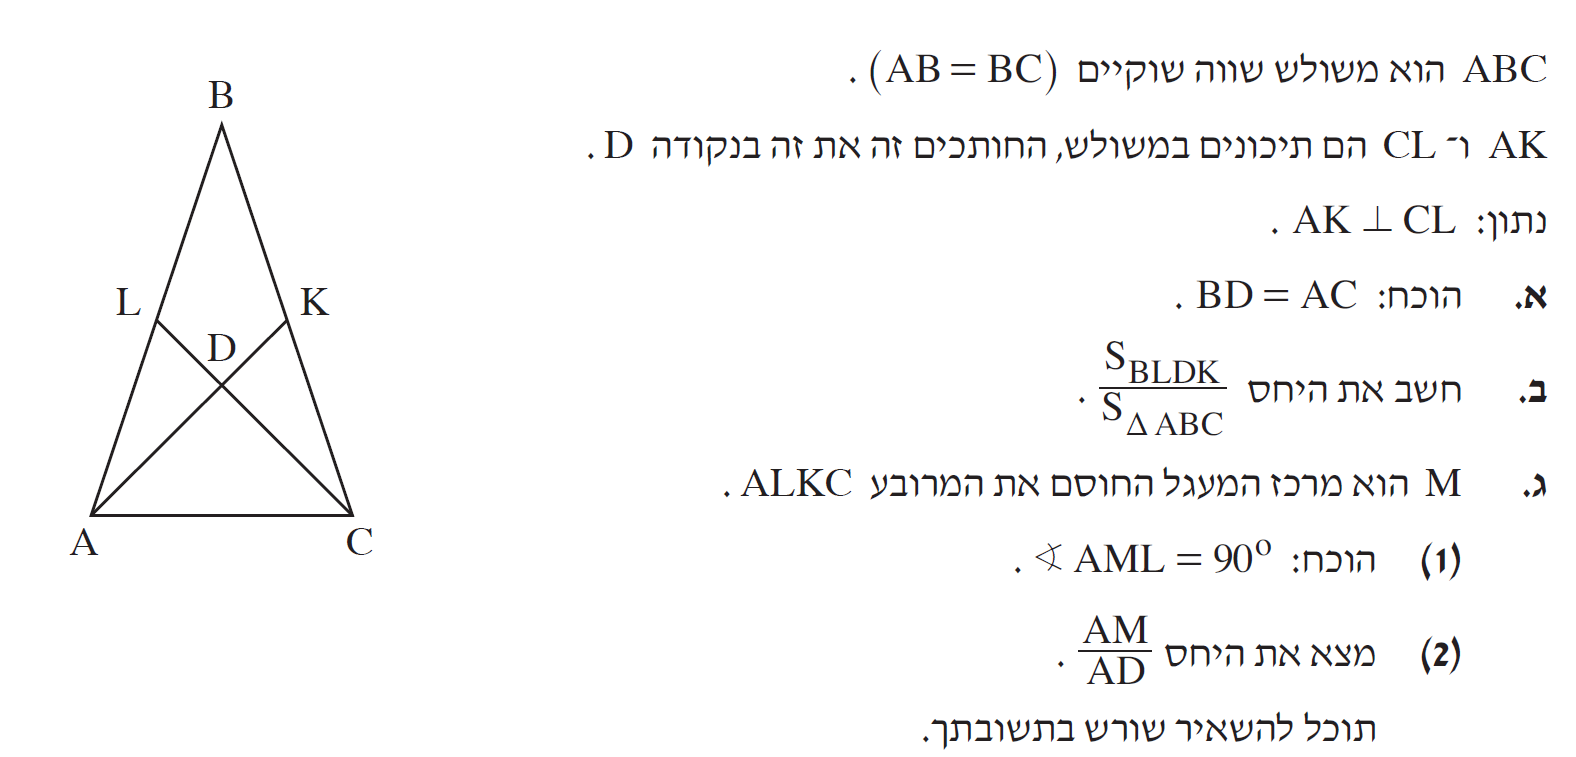
\includegraphics[width=\textwidth]{summer-2018b-4}
\end{center}
\vspace{-8mm}
\textbf{סעיף א}

כאשר יש תיכונים נחתכים מיד חושבים על משפט
$45$
"שלושת התיכונים במשולש נחתכים בנקודה אחת", ובמשפט
$46$
"נקודת חיתוך התיכונים מחלקת כל תיכון ביחס
$2:1$".
$BE$
הוא התיכון מ-%
$B$
ל-%
$AC$,
שחותך את מפגש התיכונים האחרים ב-%
$D$.
$BE\perp AC$
לפי משפט
$6$
"במשולש שווה שוקיים , חוצה זווית הראש, התיכון לבסיס והגובה לבסיס מתלכדים". מכאן קל להראות שהתיכונים
$AK,CL$
שווים.
\begin{center}
\selectlanguage{english}
\begin{tikzpicture}[scale=.7]
\draw[thick] (0,0) coordinate (A) -- (6,0) coordinate (C);
\draw[thick] (A) -- (3,8) coordinate (B) -- (C);
\coordinate (K) at ($(B) ! .5 ! (C)$);
\coordinate (L) at ($(A) ! .5 ! (B)$);
\draw[thick,name path=ak] (A) -- (K);
\draw[thick,name path=cl] (C) -- (L);
\path[name intersections={of=ak and cl,by={D}}];
\fill (A) node[below] {$A$} circle(1.5pt);
\fill (B) node[above] {$B$} circle(1.5pt);
\fill (C) node[below] {$C$} circle(1.5pt);
\fill (D) node[above right,xshift=-2pt,yshift=8pt] {$D$} circle(1.5pt);
\fill (K) node[right] {$K$} circle(1.5pt);
\fill (L) node[left] {$L$} circle(1.5pt);
\draw[rotate=-45] (D) rectangle +(7pt,7pt);
\draw[dashed,thick] (B) |- (A);
\coordinate (E) at ($(A)!.5!(C)$);
\fill (E) node[below] {$E$} circle(1.5pt);
\draw (E) rectangle +(7pt,7pt);
\path (A) -- node[right,yshift=-4pt] {$2a$} (D) -- node[right,yshift=-4pt] {$a$} (K);
\path (C) -- node[left,yshift=-4pt] {$2a$} (D) -- node[left,yshift=-4pt] {$a$} (L);
\path (B) -- node[left] {$2b$} (D) -- node[left] {$b$} (E);
\path (A) -- node[below] {$b?$} (E);
\path (E) -- node[below] {$b?$} (C);
\end{tikzpicture}
\end{center}
אם נוכיח ש-%
$AE=EC=DE$,
נוכיח ש-% 
$BD=2b=2DE=AE+ED=AC$.
לפי משפט
$6$,
$BE$
הוא חוצה זווית של
$\angle ABC$,
וגם של
$\angle ADC$
כי חוצה הזווית והתיכון מתלכדים. נתון ש-%
$AK\perp CL$
כך ש-%
$\angle ADC=90^\circ$,
ולכן 
$\angle ADE,\angle CDE$
שוות ל-%
$\frac{1}{2}\cdot 90^\circ=45^\circ$.
במשולשים ישר זווית
$\triangle ADE,\triangle CDE$,
זוויות חדות של
$45^\circ$,
ולכן גם הזוויות
$\angle DAE,\angle DCE$
שוות
$45^\circ$,
והמשולשים שווה שוקיים. מכאן ש-%
$AE=EC=DE=b$.

אפשרות אחרת, פשוטה יותר, להוכיח
$AE=EC=DE=b$
היא להשתמש במשפט
$86$
"במשולש ישר זווית התיכון ליתר שווה למחצית היתר".


\textbf{סעיף ב}

כדאי לחשב 
$S_{BLDK}$
על ידי חיסור שטח המצולע
$ALDKC$
מהשטח של
$\triangle ABC$,
כי המצולע מורכב ממשולשים ישר זווית וחישוב השטח שלהם קל מאוד:
\erh{12pt}
\begin{equationarray*}{rcl}
S_{ALDKC}&=&2S_{ADL}+S_{ADC}\\
&=&2\cdot \frac{1}{2} AD\cdot DL + \frac{1}{2} AC\cdot DE\\
&=&2a\cdot a + \frac{1}{2}\cdot 2b \cdot b\\
&=&2a^2+b^2\,.
\end{equationarray*}
אפשר להניח שהיחס המבוקש אינו תלוי באורכם של הצלעות, לכן נחפש דרך להביע את שטח המצולע
$S_{ALDKC}$
כפונקציה של
$b$
בלבד. ממשפט פיתגורס על
$\triangle ADE$:
\erh{12pt}
\begin{equationarray*}{rcl}
b^2+b^2&=&(2a)^2=4a^2\\
%b^2&=&2a^2\\
S_{ALDKC}&=&2a^2+b^2=2\cdot\frac{1}{4}(b^2+b^2)+ b^2=2b^2\\
S_{ABC}&=&\frac{1}{2}AC\cdot BE= \frac{1}{2}2b\cdot 3b=3b^2\\
S_{BLDK}&=&S_{ABC}-S_{ALDKC}=3b^2-2b^2=b^2\\
\frac{S_{BLDK}}{S_{ABC}}&=&\frac{b^2}{3b^2}=\frac{1}{3}\,.
\end{equationarray*}

\textbf{סעיף ג}
$1$

לא התקדמתי בפתרון עד שציירתי ציור חדש עם המעגל וראיתי שהזווית ההיקפית
$\angle LKA$
נשענת על המיתר עליו נשענת הזווית המרכזית
$\angle AML$,
כך ש-%
$\angle AML=2\angle LKA$
לפי משפט
$69$
"במעגל, זווית היקפית שווה למחצית הזווית המרכזית הנשענת על אותה הקשת". אבל לפי משפט
$14$
"קטע אמצעים במשולש מקביל לצלע השלישית ושווה למחציתה",
$LK\|AC$.
$\angle KAC=\angle LKA=\alpha$
לפי זוויות מתחלפות, והוכחנו בסעיף הקודם ש-%
$\alpha = 45^\circ$,
לכן,
$\angle AML = 2\alpha=90^\circ$.

\vspace{-1mm}
\begin{center}
\selectlanguage{english}
\begin{tikzpicture}
\clip (-1,-2.2) rectangle +(8,7);
\draw[thick] (0,0) coordinate (A) -- (6,0) coordinate (C);
\path (A) -- (3,8) coordinate (B) -- (C);
\coordinate (K) at ($(B) ! .5 ! (C)$);
\coordinate (L) at ($(A) ! .5 ! (B)$);
\path[name path=ak] (A) -- (K);
\draw[thick,name path=cl] (C) -- (L);
\path[name intersections={of=ak and cl,by={D}}];
\fill (A) node[below,xshift=-4pt] {$A$} circle(1.5pt);
\fill (C) node[below,xshift=4pt] {$C$} circle(1.5pt);
\fill (D) node[above] {$D$} circle(1.5pt);
\fill (K) node[right,xshift=4pt] {$K$} circle(1.5pt);
\fill (L) node[left,xshift=-4pt] {$L$} circle(1.5pt);
\draw[rotate=135] (D) rectangle +(7pt,7pt);
\tkzCircumCenter(A,L,K)\tkzGetPoint{M}
\tkzDrawCircle[thick,name path=circle](M,A)
\fill (M) node[above right] {$M$} circle(1.5pt);
\draw[rotate=110] (M) rectangle +(7pt,7pt);
\draw[thick] (A) -- (M);
\draw[thick,name path=ml] (M) -- (L);
\path[name intersections={of=ak and ml,by={G}}];
\fill (G) node[left,xshift=-4pt] {$G$} circle(1.5pt);
\draw[thick] (A) -- (L) -- (K) -- (C);
\draw[thick] (A) -- (K);
\node[below left,xshift=-8pt] at (K) {$\alpha$};
\node[left,xshift=-6pt,yshift=4pt] at (M) {$2\alpha$};
\draw[thick] ($(A)+(10mm,0)$) arc[start angle=0,end angle=45,radius=9mm];
\node[above right,yshift=10pt,xshift=22pt] at (A) {$\alpha$};
\path (L) -- node[right] {$a$} (D);
\path (A) -- node[left,xshift=4pt,yshift=8pt] {$2a$} (D);
\end{tikzpicture}
\end{center}

\textbf{סעיף ג}
$2$

תחילה שמתי לב ש-%
$\triangle MGA\sim \triangle DGL$
כי במשלושים ישר זווית, הזוויות
$\angle MGA=\angle DGL$
קודקודיות. גישה זו לא הצליחה כי לא מצאתי דרך לבטא את הקשר בין
$AD$
לבין 
$AG, GD$.
לבסוף שמתי לב שלמשולשים
$\triangle LDA,\triangle LMA$
יתר משותף, והמשולש
$\triangle LMA$
שווה שוקיים כי שני הצלעות
$AM,ML$
הם רדיוסים. ממשפט פיתגורס:
\erh{12pt}
\begin{equationarray*}{rcl}
AM^2+ML^2&=&AL^2\\
%AM&=&ML\\
2AM^2&=&AL^2\\
LD^2+AD^2&=&AL^2\\
%LD^2&=&a^2\\
a^2+AD^2&=&2AM^2\\
%AD^2&=&4a^2\\
\frac{1}{4}AD^2+AD^2&=&2AM^2\\
\frac{AM}{AD}&=&\sqrt{\frac{5}{8}}\,.
\end{equationarray*}

%%%%%%%%%%%%%%%%%%%%%%%%%%%%%%%%%%%%%%%%%%%%%%%%%%%%%%%%%%%%%%%%%%%

\newpage

\section{קיץ תשע"ח מועד א}

\begin{center}
\selectlanguage{english}
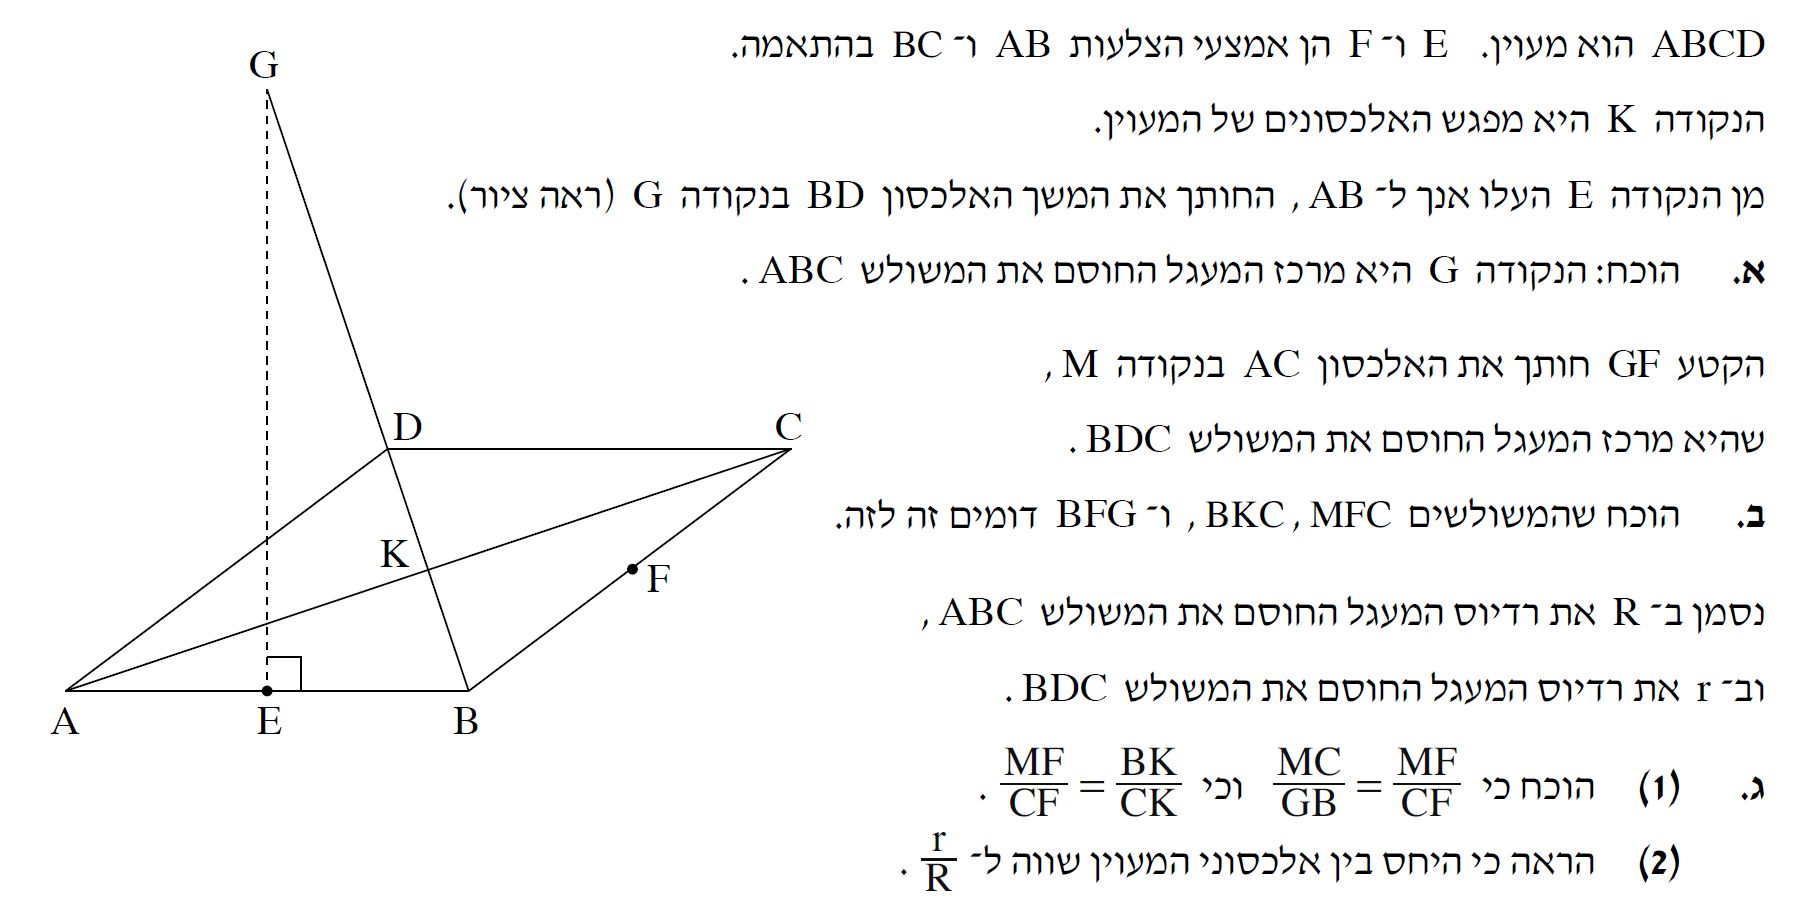
\includegraphics[width=\textwidth]{summer-2018a-4}
\end{center}
\vspace{-8mm}
\textbf{סעיף א}

כדי להוכיח שהנקודה
$G$
היא מרכז של מעגל חוסם נשתמש במשפט
$54$
"במשולש, שלושת האנכים האמצעיים נחתכים בנקודה אחת , שהיא מרכז המעגל החוסם את המשולש". צריך להוכיח ש-%
$GE,GB$
הם אנכים אמצעיים. מעוין הוא מקבילית עם צלעות שווים, וכמקבילית, ניתן להשתמש במשפט 
$28$
"במקבילית האלכסונים חוצים זה את זה". סימנו בציר את אורכי האלכסון
$AC$
ב-%
$b$.
ביחד עם משפט
$35$
"במעוין האלכסונים מאונכים זה לזה", 
$GB$
הוא אנך אמצעי ל-%
$AC$.
נתון שנקודת
$E$
היא אמצע של 
$AB$,
וש-%
$GE$
הוא אנך ל-%
%
$AB$,
ולכן
$G$
היא נקודת החיתוך של שני אנכים אמצעיים ומרכז של מעגל חוסם ל-%
$\triangle ABC$.

\begin{center}
\selectlanguage{english}
\begin{tikzpicture}[scale=.8]
\draw[thick] (0,0) coordinate (A) -- ++(40:5) coordinate (D) -- ++(5,0) coordinate (C);
\draw[thick] (A) -- ++(5,0) coordinate (B) -- (C);
\coordinate (F) at ($(B) ! .5 ! (C)$);
\coordinate (E) at ($(A) ! .5 ! (B)$);
\fill (A) node[below] {$A$} circle(1.5pt);
\fill (B) node[below] {$B$} circle(1.5pt);
\fill (C) node[above] {$C$} circle(1.5pt);
\fill (D) node[above right] {$D$} circle(1.5pt);
\fill (E) node[below] {$E$} circle(1.5pt);
\fill (F) node[right,xshift=2pt] {$F$} circle(1.5pt);
\draw[thick,name path=ac] (A) -- (C);
\path[name path=bg] (B) -- ($(B) ! 2.3 ! (D)$);
\path[name path=ge] (E) -- +(0,7.3);
\path[name intersections={of=ge and bg,by={G}}];
\fill (G) node[above] {$G$} circle(1.5pt);
\draw[dashed,thick] (G) -- (E);
\draw[thick] (G) -- (B);
\path[name intersections={of=ac and bg,by={K}}];
\fill (K) node[above,xshift=5pt,yshift=2pt] {$K$} circle(1.5pt);
\draw[rotate=110] (K) rectangle +(7pt,7pt);
\draw (E) rectangle +(7pt,7pt);
\path (A) -- node[below] {$a$} (E) -- node[below] {$a$} (B);
\path (B) -- node[right,xshift=2pt] {$a$} (F) -- node[right,xshift=2pt] {$a$} (C);
\path (A) -- node[below,near end] {$b$} (K) -- node[below,near start] {$b$} (C);
\end{tikzpicture}
\end{center}

\textbf{סעיף ב}

ההוכחה שהמשולשים דומים תהיה קל יותר אם נצייר מחדש את הציור תוך הדגשת צלעות המשולשים. לפי משפט 
$35$
האלכסון 
$AC$
הוא אנך אמצעי ל-%
$DB$.
נתון שהנקודה
$M$
היא מרכז המעגל החוסם את
$\triangle BDC$,
ולכן הנקודה
$GF$
שחותכת את 
$CK$
ב-%
$M$
היא אנך אמצעי ל-%
$BC$.
הזווית
$\alpha$
משותפת לשני משולשים ישר זווית, כך ש-%
$\triangle BKC\sim \triangle MFC$.
הזווית
$\beta$
משותפת לשני משולשים ישר זווית, כך ש-%
$\triangle BFG\sim \triangle BKC$
ו-%
$\triangle BFG\sim \triangle BKC \sim \triangle MFC$.

\begin{center}
\selectlanguage{english}
\begin{tikzpicture}[scale=.8]
\draw[thick] (0,0) coordinate (A) -- ++(40:5) coordinate (D) -- ++(5,0) coordinate (C);
\draw[thick] (A) -- ++(5,0) coordinate (B) -- (C);
\coordinate (F) at ($(B) ! .5 ! (C)$);
\coordinate (E) at ($(A) ! .5 ! (B)$);
\fill (A) node[below] {$A$} circle(1.5pt);
\fill (B) node[below] {$B$} node[above,xshift=3pt,yshift=4pt] {$\beta$}  circle(1.5pt);
\fill (C) node[above] {$C$} node[below left,xshift=-20pt,yshift=-10pt] {$\alpha$} circle(1.5pt);
\fill (D) node[above right] {$D$} circle(1.5pt);
\fill (E) node[below] {$E$} circle(1.5pt);
\fill (F) node[right] {$F$} circle(1.5pt);
\draw[thick,name path=ac] (A) -- (C);
\path[name path=bg] (B) -- ($(B) ! 2.3 ! (D)$);
\path[name path=ge] (E) -- +(0,7.3);
\path[name intersections={of=ge and bg,by={G}}];
\fill (G) node[above] {$G$} circle(1.5pt);
\draw[thick] (G) -- (B);
\path[name intersections={of=ac and bg,by={K}}];
\fill (K) node[above,xshift=5pt,yshift=2pt] {$K$} circle(1.5pt);
\draw[rotate=110] (K) rectangle +(7pt,7pt);
\draw[thick,dashed,name path=gf] (G) -- (F);
\path[name intersections={of=gf and ac,by={M}}];
\fill (M) node[below,xshift=-4pt,yshift=-4pt] {$M$} circle(1.5pt);
\draw[rotate=130] (F) rectangle +(7pt,7pt);
\draw[ultra thick] (M) -- (F) -- (C) -- cycle;
\draw[ultra thick] (B) -- (K) -- (C) -- cycle;
\draw[ultra thick] (B) -- (F) -- (G) -- cycle;
\path (B) -- node[right,xshift=4pt] {$a$} (F) -- node[right,xshift=-6pt,yshift=-10pt] {$a$} (C);
\end{tikzpicture}
\end{center}

\textbf{סעיף ג}
$(1)$

היחס: 
\[
\frac{MC}{GB}=\frac{MF}{BF}=\frac{MF}{CF}
\]
מתקבל מדמיון המשולשים
$\triangle BFG\sim \triangle MFC$
ו-%
$BF=CF$
כי 
$F$
הוא אמצע הצלע
$BC$.

מדמיון המשולשים
$\triangle BKC \sim \triangle MFC$.
מתקבל:
\erh{12pt}
\begin{equationarray*}{rcl}
\frac{MF}{BK}&=&\frac{CF}{CK}\\
\frac{MF}{CF}&=&\frac{BK}{CK}\,.
\end{equationarray*}

\textbf{סעיף ג}
$(2)$

מהנתון שהנקודה 
$M$
היא המכרז של המעגל החוסם את
$BDC$,
אנו מקבלים שהאלכסון
$MC$
שווה ל-%
$r$.
בסעיף א הוכחנו שהנקודה 
$G$
היא מרכז המעגל החוסם את
$ABC$,
ולכן 
$GB$
שווה ל-%
$R$.
נחשב את יחס הרדיוסים תוך שימוש ביחס שחישבנו בסעיף ג
$1$
ומשפט 
$29$
שהאלכסונים של מקבילית )מעוין( חוצים אחד את השני:
\[
\frac{r}{R}=\frac{MC}{GB}=\frac{BK}{CK}=\frac{DB/2}{AC/2}=\frac{DB}{AC}\,
\]


%%%%%%%%%%%%%%%%%%%%%%%%%%%%%%%%%%%%%%%%%%%%%%%%%%%%%%%%%%%%%%%%%%%
\newpage

\section{חורף תשע"ח}

\begin{center}
\selectlanguage{english}
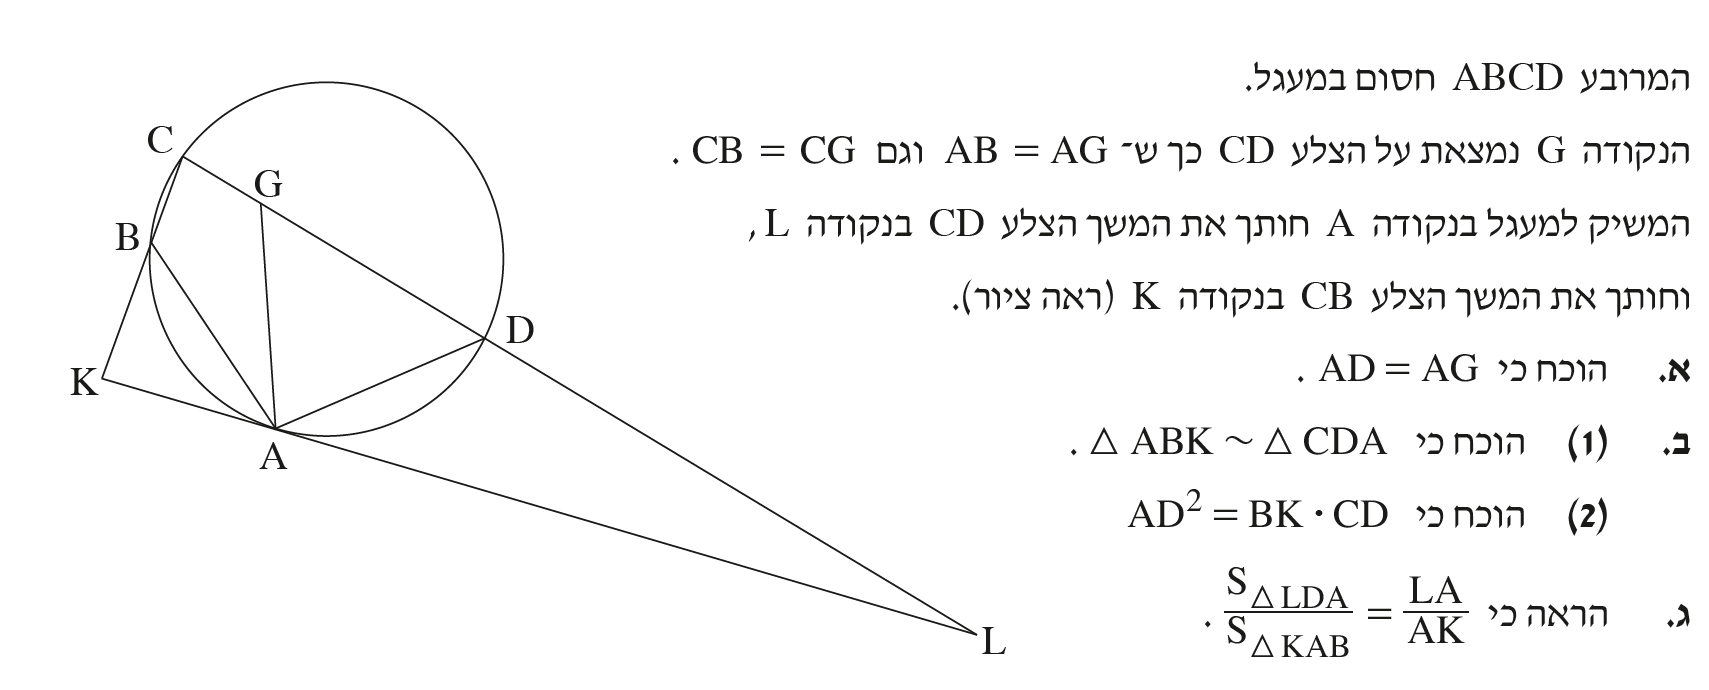
\includegraphics[width=\textwidth]{winter-2018-4}
\end{center}
\vspace{-8mm}

\textbf{סעיף א}

נתון ש-%
$AB=AG,CB=CG$
כך ש-%
$ABCG$
הוא דלתון, אבל לא ברור בשלב זה אם זה יעזור בפתרון. נתון שהמרובע 
$ABCD$
חסום במעגל, ולפי משפט
$56$
"ניתן לחסום מרובע במעגל אם ורק אם סכום זוג זוויות נגדיות שווה ל-%
$180^\circ$".
סימנו זוויות
$\alpha,\beta$
ו-%
$\alpha'=180-\alpha, \beta'=180-\beta$:
\begin{center}
\selectlanguage{english}
\begin{tikzpicture}
\coordinate (L) at (60mm,-51mm);
\fill (L) node[right] {$L$} circle(1.5pt);
\node[circle,draw,thick,name path=circle] (O) at (0,0) [minimum size=50mm] {};
\coordinate (A) at (tangent cs:node=O,point={(L)},solution=2);
\fill (A) node[below] {$A$} node[above right,yshift=8pt] {$\alpha'$} circle(1.5pt);
\path[name path=la] (L) -- ($(L)!1.4!(A)$);
\node[circle,name path=abd] (c) at (A) [minimum size=55mm] {};
\path[name intersections={of=circle and abd,by={B,D}}];
\fill (D) node[right,xshift=4pt] {$D$} node[left,xshift=-10pt,yshift=2pt] {$\beta$} circle(1.5pt);
\fill (B) node[left] {$B$} node[below right,xshift=4pt,yshift=5pt] {$\beta'$} circle(1.5pt);
\path[name path=ld] (L) -- ($(L)!2!(D)$);
\path[name intersections={of=circle and ld,by={C}}];
\fill (C) node[above left] {$C$} node[below,xshift=3pt,yshift=-6pt] {$\alpha$} circle(1.5pt);
\draw[thick,name path=lc] (L) -- (C);
\path[name path=cb] (C) -- ($(C)!2.4!(B)$);
\path[name intersections={of=cb and la,by={K}}];
\fill (K) node[below left] {$K$} circle(1.5pt);
\path[name intersections={of=abd and lc,by={dummy,G}}];
\fill (G) node[above] {$G$} circle(1.5pt);
\draw[thick] (A) -- node[left] {$a$} (B);
\draw[thick] (A) -- (D);
\draw[thick] (A) -- node[right] {$a$} (G);
\draw[thick] (L) -- (K);
\draw[thick] (C) -- node[left,xshift=-4pt] {$b$} (B);
\draw[thick] (B) -- (K);
\path (C) -- node[right,near start,xshift=4pt] {$b$} (G);
\draw ($ (A)!.15!(D) $) arc [radius=14pt,start angle=20,delta angle=94];
\draw[dashed] (B) -- (G);
\end{tikzpicture}
\end{center}
אם
$AD=AG$
המשולש
$\triangle GAD$
שווה שוקיים, ולפי הסימונים של הזוויות ננסה להוכיח ש-%
$\angle AGD=\angle ADG=\beta$.
נזכור ש-%
$ABCG$
דלתון והזוויות הצדדיות שלו שוות, כך ש:
\[
\angle AGC=\angle ABC=\beta'\,,\quad\quad \angle AGD=180-(180-\beta)=\beta\,.
\]
\vspace{-10mm}
\begin{quote}
רשימת המשפטים לבגרות לא כוללת משפט על שוויון זוויות בדלתון, אז נצטרך להוכיח אותו. דלתון מוגדר כמרובע עם שני זוגות של צלעות סמוכות שוות, כך שהוא מורכב משני משולשים שווה שוקיים המוצמדים בבסיסיהם )קו מקווקוו בציור(:
\[
\angle ABC = \angle ABG + \angle GBC = \angle AGB + \angle BGC = \angle AGC\,.
\]
\end{quote}

\textbf{סעיף ב %
$(1)$}

נדגיש בציור את המשולשים
$\triangle ABK,\triangle CDA$
שיש להוכיח שהם דומים. הוספנו לציור את הסימון
$\angle ABK=\beta$,
המשלים של 
$\angle ABC=\beta'$.
אם נמצא עוד זוג של זוויות שוות נקבל שהמשולים דומים לפי ז.ז. ננסה להוכיח ש-%
$\angle ACD=\angle BAK$.

$\angle BAK$
היא הזווית בין המשיק
$KA$
והמיתר
$AB$.
לפי משפט
$79$
"זווית בין משיק ומיתר שווה לזווית ההיקפית הנשענת על מיתר זה מצידו השני", 
$\angle BAK=\angle BCA=\gamma$.
לפי משפט
$21$
"האלכסון הראשי בדלתון חוצה את זוויות הראש ...",
$\angle BAK=\angle BCA=\angle ACD=\gamma$.
מכאן ש-%
$\triangle ABK \sim \triangle CDA$
לפי ז.ז.
\begin{center}
\selectlanguage{english}
\begin{tikzpicture}
\coordinate (L) at (60mm,-51mm);
\node[circle,draw,name path=circle] (O) at (0,0) [minimum size=50mm] {};
\coordinate (A) at (tangent cs:node=O,point={(L)},solution=2);
\fill (A) node[below] {$A$} circle(1.5pt);
\path[name path=la] (L) -- ($(L)!1.4!(A)$);
\node[circle,name path=abd] (c) at (A) [minimum size=55mm] {};
\path[name intersections={of=circle and abd,by={B,D}}];
\fill (D) node[right,xshift=4pt] {$D$} node[left,xshift=-10pt,yshift=2pt] {$\beta$} circle(1.5pt);
\fill (B) node[left] {$B$} node[right,yshift=1pt] {$\beta'$} node[below,xshift=2pt,yshift=-8pt] {$\beta$} circle(1.5pt);
\path[name path=ld] (L) -- ($(L)!2!(D)$);
\path[name intersections={of=circle and ld,by={C}}];
\fill (C) node[above left] {$C$} circle(1.5pt);
\path[name path=lc] (L) -- (C);
\path[name path=cb] (C) -- ($(C)!2.4!(B)$);
\path[name intersections={of=cb and la,by={K}}];
\fill (K) node[below left] {$K$} circle(1.5pt);
\path[name intersections={of=abd and lc,by={dummy,G}}];
\fill (G) node[above] {$G$} circle(1.5pt);
\draw (A) -- (G);
\draw (C) -- (B);
\draw[very thick] (A) -- (B);
\draw[very thick] (A) -- (D);
\draw[very thick] (B) -- (K);
\draw[very thick] (C) -- (A);
\draw[very thick] (A) -- (K);
\draw[very thick] (D) -- (C);
\node at ($(C)+(-8.5mm,-5mm)$) {$\gamma$};
\node at ($(C)+(-6mm,-5.2mm)$) {$?$};
\draw[->] ($(C)+(-4mm,-4mm)$) -- +(13pt,0);
\draw[->] ($(C)+(-4mm,-6mm)$) -- +(22pt,0);
\node at ($(A)+(-8.5mm,-2mm)$) {$\gamma$};
\node at ($(A)+(-6mm,-2.2mm)$) {$?$};
\draw[->] ($(A)+(-7mm,0mm)$) -- +(8pt,12pt);
\end{tikzpicture}
\end{center}
\vspace*{-25mm}
דרך אחרת להוכיח ש-%
$\angle BCA=\angle ACD$
היא לשים לב ש-%
$AB=AG=AD$.
נשתמש במשפט
$63$
"במעגל, מיתרים שווים זה לזה אם ורק אם שתי הקשתות המתאימות להם שוות זו לזו" ומשפט
$71$
"במעגל, לקשתות שוות מתאימות זוויות היקפיות שוות", ונקבל
$\angle BCA=\angle ACD$.

\textbf{סעיף ב %
$(2)$}

לפי 
$\triangle ABK \sim \triangle CDA$
שהוכחנו בהחלק הראשון של הסעיף ולפי
$AB=AD$:
\erh{4pt}
\begin{equationarray*}{rcl}
\frac{AB}{CD}&=&\frac{BK}{AD}\\
AB\cdot AD &=& BK\cdot CD\\
AD^2 &=& BK\cdot CD\,.
\end{equationarray*}

\newpage

\textbf{סעיף ג}

$LA,AK$
הם הבסיסים של המשולשים
$\triangle LDA, \triangle KAB$
כך שנקבל את היחס המבוקש אם נוכיח שהגבהים שווים. הוכחנו שהיתרים ב-%
$\triangle ADN,\triangle ABM$
שווים
$AB=AD=a$,
כך שנשאר רק להוכיח שהזוויות שוות
$\angle BAK=\angle DAL=\gamma$.
הוכחנו ש-%
$\angle BAK=\angle DCA=\gamma$,
ו-%
$\angle DAL$
היא הזווית בין המשיק
$LA$
והמיתר 
$AD$.
הזווית
$\angle DCA$
נשענת על מיתר זה, כך ש-%
$\angle DCA=\angle DAL$
לפי משפט
$79$,
ו-%
$\angle BAK=\angle DCA=\angle DAL=\gamma$.
כעת ניתן לחשב את השטחים:
\erh{12pt}
\begin{equationarray*}{rcl}
\frac{S_{LDA}}{S_{KAB}}&=&\frac{(LA\cdot DN)/2}{(AK\cdot BM)/2}\\
DN&=&AD\sin \angle DAL=a\sin\gamma\\
BM&=&AB\sin \angle BAK=a\sin\gamma\\
\frac{S_{LDA}}{S_{KAB}}&=&\frac{LA}{AK}\,.
\end{equationarray*}


\begin{center}
\selectlanguage{english}
\begin{tikzpicture}
\coordinate (L) at (60mm,-51mm);
\fill (L) node[right] {$L$} circle(1.5pt);
\node[circle,draw,thick,name path=circle] (O) at (0,0) [minimum size=50mm] {};
\coordinate (A) at (tangent cs:node=O,point={(L)},solution=2);
\fill (A) node[below] {$A$} circle(1.5pt);
\path[name path=la] (L) -- ($(L)!1.4!(A)$);
\node[circle,name path=abd] (c) at (A) [minimum size=55mm] {};
\path[name intersections={of=circle and abd,by={B,D}}];
\fill (D) node[right,xshift=4pt] {$D$} circle(1.5pt);
\fill (B) node[left] {$B$} circle(1.5pt);
\path[name path=ld] (L) -- ($(L)!2!(D)$);
\path[name intersections={of=circle and ld,by={C}}];
\fill (C) node[above left] {$C$} circle(1.5pt);
\draw[thick,name path=lc] (L) -- (C);
\path[name path=cb] (C) -- ($(C)!2.4!(B)$);
\path[name intersections={of=cb and la,by={K}}];
\fill (K) node[below,yshift=-2pt] {$K$} circle(1.5pt);
\path[name intersections={of=abd and lc,by={dummy,G}}];
\draw[thick] (A) -- node[right,near end] {$a$} (B);
\draw[thick] (A) -- node[above] {$a$} (D);
\draw[thick] (L) -- ($(L)!1.1!(K)$);
\draw[thick] (B) -- (K);
\draw[thick] (A) -- (C);
\draw[thick,dashed] (D) -- ($(A)!(D)!(L)$) coordinate (N);
\draw[thick,dashed] (B) -- ($(A)!(B)!(L)$) coordinate (M);
\fill (N) node[below] {$N$} circle(1.5pt);
\fill (M) node[below left] {$M$} circle(1.5pt);
\draw[rotate=-22] (N) rectangle +(7pt,7pt);
\draw[rotate=70] (M) rectangle +(7pt,7pt);
\node at ($(C)+(-8.5mm,-5mm)$) {$\gamma$};
\draw[->] ($(C)+(-4mm,-4mm)$) -- +(22pt,0);
\node at ($(A)+(-8.5mm,-2mm)$) {$\gamma$};
\draw[->] ($(A)+(-7mm,0mm)$) -- +(8pt,12pt);
\node at ($(A)+(6mm,-8mm)$) {$\gamma$};
\node at ($(A)+(9mm,-8mm)$) {$?$};
\draw[->] ($(A)+(6.1mm,-5.8mm)$) -- +(12pt,18pt);
\end{tikzpicture}
\end{center}


%%%%%%%%%%%%%%%%%%%%%%%%%%%%%%%%%%%%%%%%%%%%%%%%%%%%%%%%%%%%%%%%%%%


\newpage

\section{קיץ תשע"ז מועד ב}

\begin{center}
\selectlanguage{english}
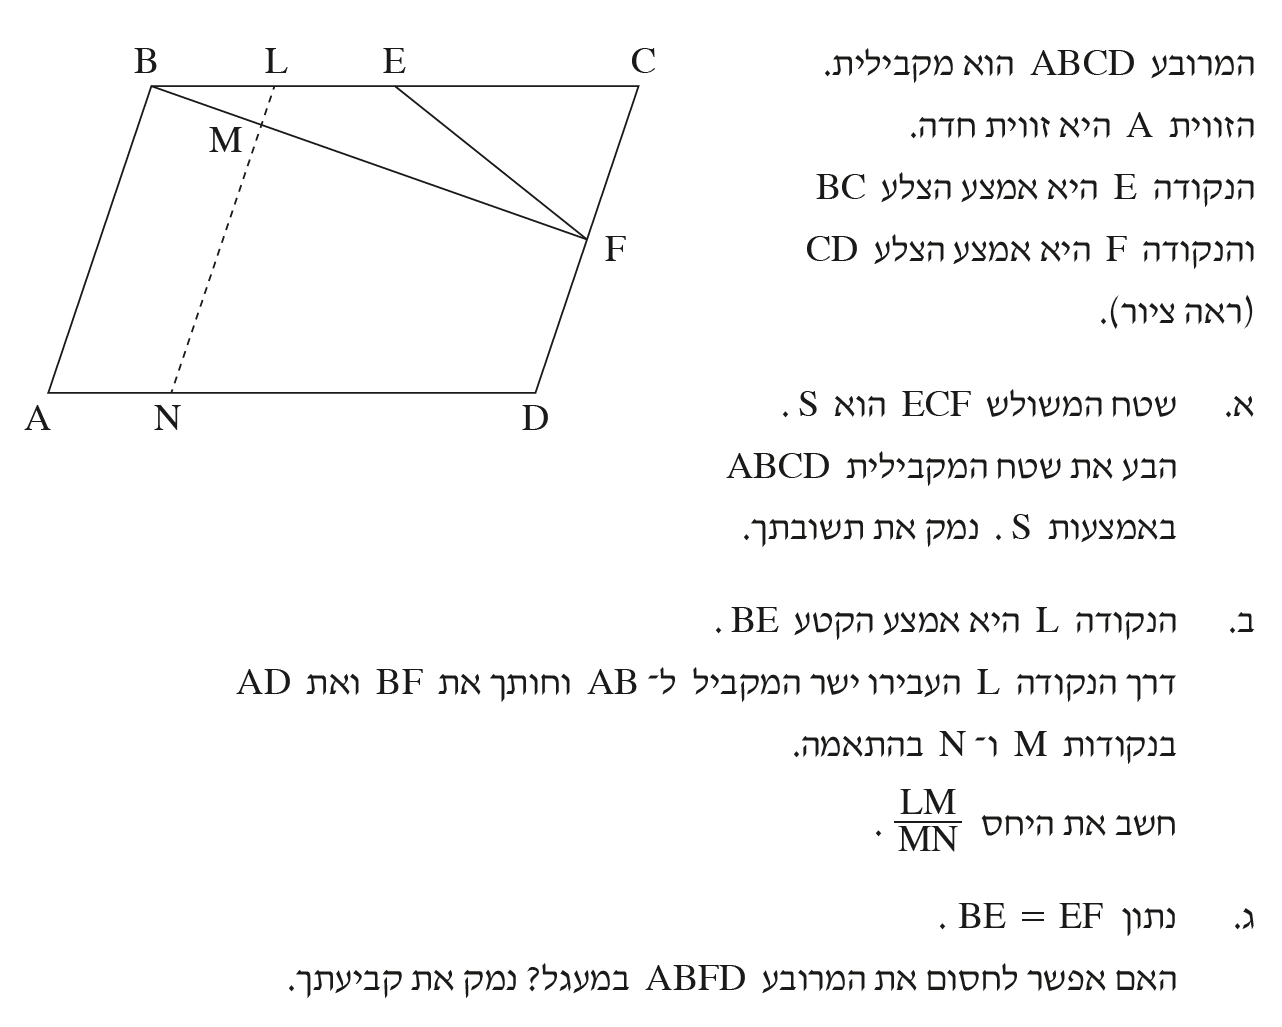
\includegraphics[width=.8\textwidth]{summer-2017b-4}
\end{center}
\vspace{-8mm}
\textbf{סעיף א}

כדי לחשב את שטח המקבילית באמצעות שטח של משולש נפרק את המקבילית למשולשים. יהי 
$GF$
מקביל ל-%
$BC$
ו-%
$EH$
מקביל ל-%
$CD$.
לפי זוויות מתאימות ומשלימות, המרובעים 
$BEHG,ECFH$
הם מקביליות. בגלל ש-%
$E$
היא נקודת האמצע של
$BC$,
$H$
הוא נקודת האמצע של
$GF=BC$.
מכאן שהמשולשים 
$\triangle ECF,\triangle EHF$
חופפים, ו-%
$S_{EHF}=S_{ECF}=S$.
באותה דרך נוכיח ש-%
$S_{BEH}=S_{BGH}=S$,
ולכן
$S_{BCFG}=4S$.
$GF$
הוא קו אמצעים ומחלק את המקבילית לשני חלקים ששטחם שווה, כך ש-%
$S_{ABCD}=S_{BCFG}+S_{GFDA}=8S$.

\begin{center}
\selectlanguage{english}
\begin{tikzpicture}[scale=.8]
\coordinate (B) at (0,0);
\coordinate (E) at (4,0);
\coordinate (C) at (8,0);
\draw[thick] (B) -- (C);
\draw[thick] (E) -- +(-30:4) coordinate (F);
\draw[thick] (C) -- ($(C) ! 2 ! (F)$) coordinate (D);
\draw[thick] (D) -- +(-8,0) coordinate (A) -- (B);
\fill (A) node[below left] {$A$} circle(1.5pt);
\fill (B) node[above left] {$B$} circle(1.5pt);
\fill (C) node[above right] {$C$} circle(1.5pt);
\fill (D) node[below right] {$D$} circle(1.5pt);
\fill (E) node[above] {$E$} circle(1.5pt);
\fill (F) node[right] {$F$} circle(1.5pt);
\coordinate (G) at ($(A)!.5!(B)$);
\fill (G) node[left] {$G$} circle(1.5pt);
\draw[thick,dashed] (G) -- (F);
\coordinate (H) at ($(G)!.5!(F)$);
\fill (H) node[below] {$H$} circle(1.5pt);
\draw[thick,dashed] (E) -- (H) -- (B);
\end{tikzpicture}
\end{center}
\vspace{-3mm}
הוכחה אחרת היא להשתמש במשפט
$5$%
א "שטח מקבילית שווה למכפלת צלע המקבילית בגובה לצלע זו". הגובה של המקבילית באורך כפול מהגובה של המשולש לפי דמיון המשולשים 
$\triangle FCK, \triangle DCJ$:
\vspace{-3mm}
\erh{10pt}
\begin{equationarray*}{rcl}
S_{ECF}&=&\frac{1}{2}ah=S\\
S_{ABCD}&=&2a\cdot 2h=4ah=8S\,.
\end{equationarray*}
\begin{center}
\selectlanguage{english}
\begin{tikzpicture}[scale=.8]
\coordinate (B) at (0,0);
\coordinate (E) at (4,0);
\coordinate (C) at (8,0);
\draw[thick] (B) -- (C);
\draw[thick] (E) -- +(-30:4) coordinate (F);
\draw[thick] (C) -- ($(C) ! 2 ! (F)$) coordinate (D);
\draw[thick] (D) -- +(-8,0) coordinate (A) -- (B);
\fill (A) node[below left] {$A$} circle(1.5pt);
\fill (B) node[above left] {$B$} circle(1.5pt);
\fill (C) node[above right] {$C$} circle(1.5pt);
\fill (D) node[below right] {$D$} circle(1.5pt);
\fill (E) node[above] {$E$} circle(1.5pt);
\fill (F) node[below left] {$F$} circle(1.5pt);
\draw[thick,dashed,name path=dj] (D) -- +(2.5,0);
\draw[thick,dashed,name path=cj] (C) -- ($(A)!(C)!(D)$);
\path[name intersections={of=dj and cj,by={J}}];
\fill (J) node[below] {$J$} circle(1.5pt);
\draw (J) rectangle +(7pt,7pt);
\coordinate (K) at ($(C)!.5!(J)$);
\fill (K) node[right] {$K$} circle(1.5pt);
\path (E) -- node[above] {$a$} (C);
\path (A) -- node[below] {$2a$} (D);
\draw[thick,dashed] (F) -- (K);
\draw[<->] ($(C)+(.9,0)$) -- node[fill=white] {$h$} ($(K)+(.9,0)$);
\draw[<->] ($(C)+(1.4,0)$) -- node[fill=white] {$2h$} ($(J)+(1.4,0)$);
\end{tikzpicture}
\end{center}
\textbf{סעיף ב}
נקבל יחס בין קטעי קו אם נמצא משולשים דומים שקטעי הקו הם צלעות שלהם. בציור להלן הדגשתי משולשים שיכולים להתאים. קטע האמצעים במקבילית מקביל לבסיסים
$BC\|GF$,
ומזוויות מתחלפות
$\angle LBM=\angle MFK$
וזוויות קודקודיות
$\angle LMB=\angle KMF$,
נקבלים
$\triangle LMB \sim \triangle KMF$.
בציור רשמנו את אורכי הקטעים תוך שימוש בנעלמים
$a,b,c$.

\begin{center}
\selectlanguage{english}
\begin{tikzpicture}[scale=.8]
\coordinate (B) at (0,0);
\coordinate (E) at (4,0);
\coordinate (C) at (8,0);
\draw[thick] (B) -- (C);
\path (E) -- +(-30:4) coordinate (F);
\draw[thick] (C) -- ($(C) ! 2 ! (F)$) coordinate (D);
\draw[thick] (D) -- +(-8,0) coordinate (A) -- (B);
\draw[thick,name path=bf] (B) -- (F);
\fill (A) node[below left] {$A$} circle(1.5pt);
\fill (B) node[above left] {$B$} circle(1.5pt);
\fill (C) node[above right] {$C$} circle(1.5pt);
\fill (D) node[below right] {$D$} circle(1.5pt);
%\fill (E) node[above] {$E$} circle(1.5pt);
\fill (F) node[right] {$F$} circle(1.5pt);
\coordinate (G) at ($(A)!.5!(B)$);
\fill (G) node[left] {$G$} circle(1.5pt);
\draw[thick,dashed,name path=gf] (G) -- (F);
\coordinate (L) at (2,0);
\draw[thick,dashed,name path=ln] (L) -- ($(A)!.25!(D)$) coordinate (N);
\fill (L) node[above] {$L$} circle(1.5pt);
\fill (N) node[below] {$N$} circle(1.5pt);
\path[name intersections={of=bf and ln,by={M}}];
\fill (M) node[below left] {$M$} circle(1.5pt);
\path[name intersections={of=gf and ln,by={K}}];
\fill (K) node[below left ] {$K$} circle(1.5pt);
\draw[thick] (L) -- (K);
\draw[thick] (K) -- (F);
\draw[ultra thick] (B) -- node[above] {$a$} (L);
\path (B) -- node[left] {$b$} (G);
\path (G) -- node[left] {$b$} (A);
\path (K) -- node[left] {$b$} (N);
\draw[ultra thick] (K) -- node[below] {$3a$} (F);
\draw[ultra thick] (L) -- node[right] {$c$} (M);
\draw[ultra thick] (M) -- node[left] {$b-c$} (K);
\draw[ultra thick] (B) -- (F);
\end{tikzpicture}
\end{center}
\vspace{-3ex}
\erh{10pt}
\begin{equationarray*}{rcl}
\frac{c}{b-c}&=&\frac{a}{3a}=\frac{1}{3}\\
b&=&4c\\
\frac{LM}{MN}&=&\frac{c}{2b-c}\\
&=&\frac{a}{2\cdot 4c-c}\\
&=&\frac{1}{7}\,.
\end{equationarray*}

\newpage

\textbf{סעיף ג}

כדי לחסום את המרובע
$ABFD$,
לפי משפט 
$56$
"ניתן לחסום מרובע במעגל אם ורק אם סכום זוג זוויות נגדיות שווה ל-%
$180^\circ$.

בציור להלן הוספתי את הנתון 
$BE=EF$.
ראיתי פתרון שמשתמש במשפט
$86$
"במשולש ישר זווית התיכון ליתר שווה למחצית היתר" כדי להוכיח ש-%
$\angle BFC=90^\circ$.
הוכחה זו בעייתית כי משפט
$86$
לא מנוסח כ-"אם ורק אם". לא קשה להוכיח את הכיוון ההפוך כי כל הנקודות הנמצאות במרחק שווה מנקודה 
$E$
נמצאות על מעגל שמרכזו 
$E$.

אפשר לפתור את השאלה ללא שימוש במשפט
$86$
תוך שימוש בעובדות ש: )א( המרובע
$ABCD$
הוא מקבילית, )ב( המשולשים 
$\triangle BEF,\triangle CEF$
שווה שוקיים, )ג( זוויות משלימות ב-%
$E$,
נסמן את הזוויות של המשולש שווה שוקיים
$\triangle BEF$
ב-%
$\alpha$.
מכאן ש-%
$\angle BEF=180-2\alpha$
ולפי זוויות משלימות
$\angle CEF=2\alpha$.
גם משולש 
$\triangle CEF$
הוא שווה שוקיים כך ש-%
$\angle ECF=\angle EFC=90-\alpha$.
ניתן לחבר זוויות ולקבל
$\angle BFC=\angle BFD=90$.

לפי משפט
$26$
"במקבילית כל שתי זוויות נגדיות שוות זו לזו" 
$\angle BAD=\angle BCD=90-\alpha$.
כדי לחסום את המרובע
$ABFD$
חייב להתקיים:
\[
\angle BFD + \angle BAD = 90 + (90-\alpha) = 180-\alpha=180\,.
\]
נתון ש-%
$\angle BAD$
היא זווית חדה שהיא פחות מ-%
$90^\circ$:
\erh{0pt}
\begin{equationarray*}{rcl}
90-\alpha&<&90\\
\alpha&>&0\\
180-\alpha&<&180\,,
\end{equationarray*}
שסותר את הדרישה 
$180-\alpha=180$,
לכן אי אפשר לחסום את המרובע במעגל.
\begin{center}
\selectlanguage{english}
\begin{tikzpicture}[scale=1]
\coordinate (B) at (0,0);
\coordinate (E) at (4,0);
\coordinate (C) at (8,0);
\draw[thick] (B) -- (C);
\draw[thick] (E) -- +(-30:4) coordinate (F);
\draw[thick] (C) -- ($(C) ! 2 ! (F)$) coordinate (D);
\draw[thick] (D) -- +(-8,0) coordinate (A) -- (B);
\draw[thick,name path=bf] (B) -- (F);
\fill (A) node[below left] {$A$} circle(1.5pt);
\fill (B) node[above left] {$B$} circle(1.5pt);
\fill (C) node[above right] {$C$} circle(1.5pt);
\fill (D) node[below right] {$D$} circle(1.5pt);
\fill (E) node[above] {$E$} circle(1.5pt);
\fill (F) node[right] {$F$} circle(1.5pt);
\path (B) -- node[above] {$a$} (E) -- node[above] {$a$} (C);
\path (E) -- node[above] {$a$} (F);
\draw[rotate=165] (F) rectangle +(7pt,7pt);
\node[below right,xshift=28pt,yshift=2pt] at (B) {$\alpha$};
\node[above left,xshift=-28pt,yshift=8pt] at (F) {$\alpha$};
\node[below left,xshift=0pt,yshift=2pt] at (C) {$90-\alpha$};
\node[above right,xshift=6pt,yshift=2pt] at (A) {$90-\alpha$};
\node[below left,xshift=-10pt,yshift=-2pt] at (F) {$90$};
\node[above,xshift=40pt,yshift=2pt] at (F) {$90-\alpha$};
\node[below left,xshift=4pt,yshift=2pt] at (E) {$180-2\alpha$};
\node[below right,xshift=16pt,yshift=2pt] at (E) {$2\alpha$};
\draw[->] ($(F)+(20pt,10pt)$) -- +(-25pt,0);
\end{tikzpicture}
\end{center}

%%%%%%%%%%%%%%%%%%%%%%%%%%%%%%%%%%%%%%%%%%%%%%%%%%%%%%%%%%%%%%%%%%%

\newpage

\section{קיץ תשע"ז מועד א}

\begin{center}
\selectlanguage{english}
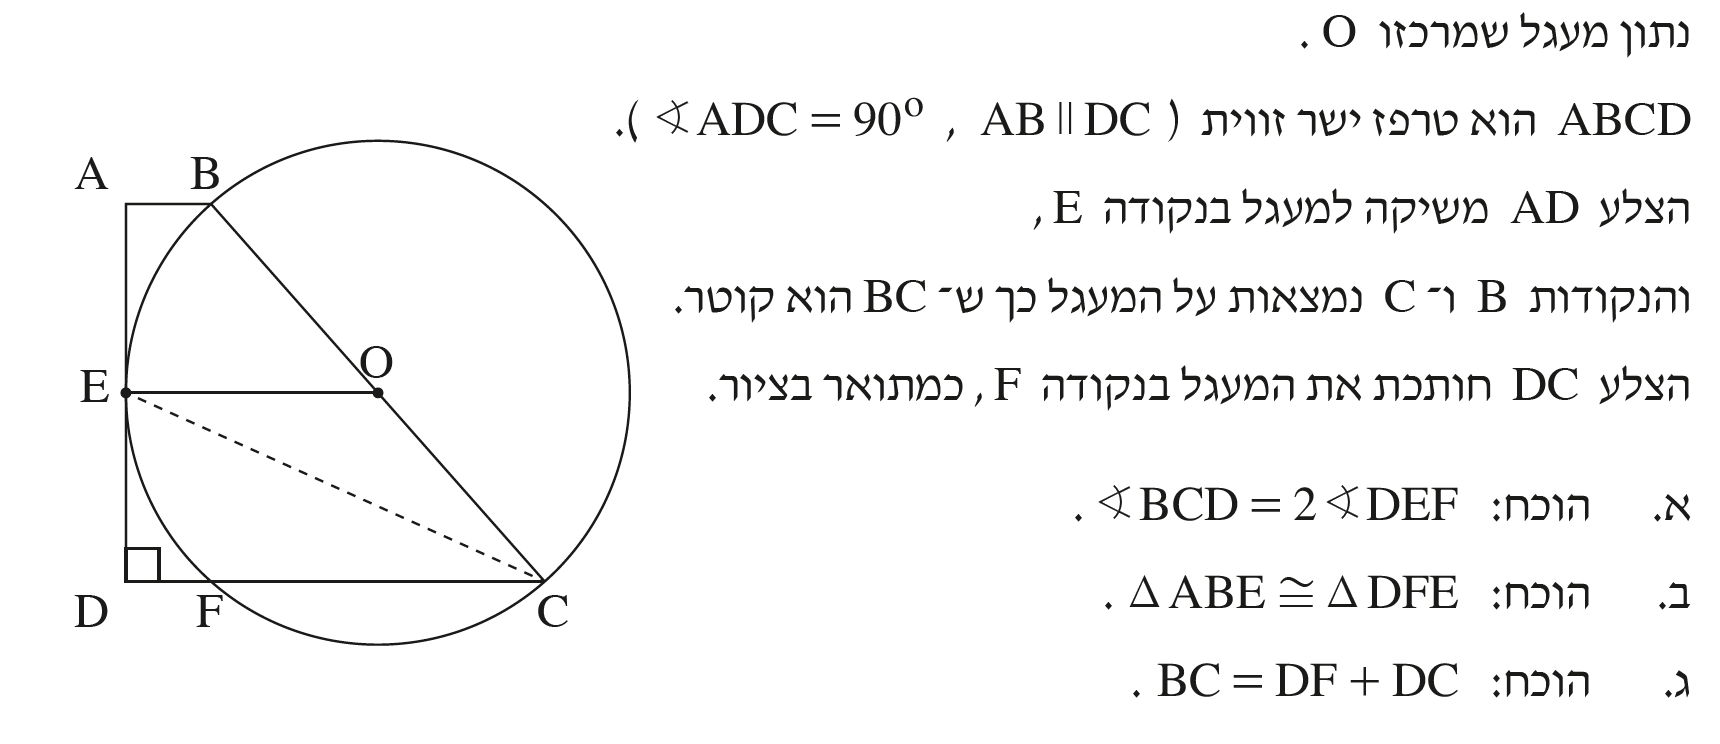
\includegraphics[width=\textwidth]{summer-2017a-4}
\end{center}
\vspace{-6mm}

\textbf{סעיף א}

השאלה שואלת על זוויות ויש לנו קווים מקבילים, משיק, זווית ישרה. ננסה להסיק מסקנות על זזויות. מחברי השאלה סיפקו רמז: הקו 
$EC$.
$\angle DEF$
היא הזווית בין המשיק
$ED$
לבין במיתר 
$EF$
המסומן בציור. לפי משפט 
$79$
"זווית בין משיק ומיתר שווה לזווית ההיקפית הנשענת על מיתר זה מצידו השני",
$\angle DEF$
שווה להזווית ההיקפית
$\angle ECF$.
סימנו את שתי הזוויות ב-%
$\alpha$.

נקבל את הערך של
$\angle BCD$
אם נידע את ערכה של
$\angle ECO$.
נתון ש-%
$AB\|DC,\angle ADC=90^\circ$.
המשיק מאונך לרדיוס
$EO$,
ולכן, 
$EO\|DC,EO\perp AD$,
ו-%
$\angle OEC=\alpha=\angle ECB$
לפי זווית מתחלפות. המשולש
$\triangle ECO$
שווה שוקיים ולכן
$\angle ECO=\alpha$,
ן-%
$\angle BCD=2\alpha= 2\angle{DEF}$.

\begin{center}
\selectlanguage{english}
\begin{tikzpicture}[scale=.9]
\coordinate (O) at (0,0);
\fill (O) node[right] {$O$} circle(1.5pt);
\draw[thick,name path=circle] (O) circle(3cm);
\coordinate (E) at (-3,0);
\fill (E) node[left] {$E$} node[below right,xshift=22pt] {$\alpha?$} circle(1.5pt);
\draw[thick] (E) -- +(0,2.5) coordinate (A);
\fill (A) node[above left] {$A$} circle(1.5pt);
\draw[thick] (E) -- +(0,-2.5) coordinate (D);
\fill (D) node[below left] {$D$} circle(1.5pt);
\path[name path=db] (D) -- +(6,0);
\path[name intersections={of=db and circle,by={F,C}}];
\fill (C) node[below right] {$C$} node[above left,xshift=-18pt] {$\alpha$} node[above left,xshift=-16pt,yshift=16pt] {$\alpha?$} circle(1.5pt);
\fill (F) node[below] {$F$} circle(1.5pt);
\path[name path=ab] (A) -- +(2,0);
\path[name intersections={of=ab and circle,by={B}}];
\fill (B) node[above] {$B$} circle(1.5pt);
\draw[thick] (A) -- (B) -- (C) -- (D);
\draw[thick] (E) -- node[above] {$r$} (O) -- node[right] {$r$} (C);
\draw[thick,dashed] (C) -- (E) -- (F);
\node at (-40mm,-5mm) {$\alpha$};
\draw[->] (-39mm,-5mm) -- +(11mm,0);
\draw (E) rectangle +(7pt,7pt);
\draw (D) rectangle +(7pt,7pt);
\draw[rotate=-90] (A) rectangle +(7pt,7pt);
\end{tikzpicture}
\end{center}
הוכחה אחרת משתמשת במשפט
$103$
"אם מנקודה שמחוץ למעגל יוצאים חותך ומשיק, אז מכפלת החותך בחלקו החיצוני שווה לריבוע המשיק". לכן:
\vspace{-3mm}
\erh{10pt}
\begin{equationarray*}{rcl}
ED^2&=&DC\cdot DF\\
\frac{ED}{DF}&=&\frac{DC}{ED}\\
\triangle EDF &\sim& \triangle CDE\,.
\end{equationarray*}
נשתמש במשפט
$69$
"במעגל, זווית היקפית שווה למחצית הזווית המרכזית הנשענת על אותה הקשת", בזוויות המתחלפות 
$\angle BOE=\angle BCD$
ובדמיון המשולשים 
$\triangle EDF \sim \triangle CDE$
שכבר הוכחנו:
\erh{6pt}
\begin{equationarray*}{rcl}
\angle BCD &=& \angle BOE\\
&=& 2\cdot \angle BCE\\
\angle ECD &=& \angle BCD-\angle BCE\\
&=&\angle BCD - \angle BCD/2\\
\angle DEF &=& \angle BCD/2\,.
\end{equationarray*}
\vspace{-6mm}

\textbf{סעיף ב}

שני המשולשים
$\triangle ABE\cong\triangle DFE$
כי הם ישר זווית וצלע באחד המשולשים שווים לזווית וצלע מקבילים במשלוש השני, כי ביחד עם הזווית הישרה יש חפיפה לפי ז.צ.ז. 

נתון ש-%
$BC$
הוא קוטר שמרכזו 
$O$
ולכן
$BO=OC=r$.
נפעיל את השפט
$44$
"בטרפז, ישר החוצה שוק אחת ומקביל לבסיסים, חוצה את השוק השנייה" על הטרפז
$ABCD$,
כדי לקבל
$AE=DE=a$.
נצייר את המיתר
$BE$
ונקווה שהזווית 
$\angle AEB$
בין המיתר ומשיק יהיה שווה לזווית
$\angle DEF=\alpha$
במשלוש השני. לפי משפט
$79$,
$\angle AEB=\angle ECO$,
הזווית ההיקפית.
אבל כבר הוכחנו שזווית זו שווה ל-%
$\angle ECO=\angle DEF=\alpha$.
\begin{center}
\selectlanguage{english}
\begin{tikzpicture}[scale=.9]
\coordinate (O) at (0,0);
\fill (O) node[right] {$O$} node[above left,xshift=-4pt] {$2\alpha$} circle(1.5pt);
\draw[thick,name path=circle] (O) circle(3cm);
\coordinate (E) at (-3,0);
\fill (E) node[left] {$E$} circle(1.5pt);
\draw[thick] (E) -- node[left] {$a$} +(0,2.5) coordinate (A);
\fill (A) node[above left] {$A$} circle(1.5pt);
\draw[thick] (E) -- node[left] {$a$} +(0,-2.5) coordinate (D);
\fill (D) node[below left] {$D$} circle(1.5pt);
\path[name path=db] (D) -- +(6,0);
\path[name intersections={of=db and circle,by={F,C}}];
\fill (C) node[below right] {$C$} node[above left,xshift=-16pt,yshift=14pt] {$\alpha$} node[above left,xshift=-20pt,yshift=2pt] {$\alpha$} circle(1.5pt);
\fill (F) node[below] {$F$} circle(1.5pt);
\path[name path=ab] (A) -- +(2,0);
\path[name intersections={of=ab and circle,by={B}}];
\fill (B) node[above] {$B$} circle(1.5pt);
\draw[thick] (A) -- (B) -- (C) -- (D);
\draw[thick] (E) -- (O) -- node[right] {$r$} (C);
\draw[thick,dashed] (C) -- (E) -- (F);
\draw[thick,dashed] (B) -- (E);
\node at (-43mm,-5mm) {$\alpha$};
\draw[->] (-39mm,-5mm) -- +(11mm,0);
\node at (-43mm,5mm) {$\alpha?$};
\draw[->] (-39mm,5mm) -- +(11mm,0);
\draw (E) rectangle +(7pt,7pt);
\draw (D) rectangle +(7pt,7pt);
\draw[rotate=-90] (A) rectangle +(7pt,7pt);
\path (O) -- node[right] {$r$} (B);
\end{tikzpicture}
\end{center}
הוכחה אחרת מחשבת זוויות מהשולש שווה שוקיים
$\triangle BOE$.
$\angle BOE=2\alpha$
ולכן
$\angle BEO = \angle OBE = 90-\alpha$
ו-%
$\angle AEB=\alpha=\angle DEF$.
ביחד עם 
$AE,ED$,
$\triangle ABE, \triangle DFE$
חופפים.
\newpage

\textbf{סעיף ג}

האורך של 
$BC$
הוא 
$2r$,
כך שעלינו להוכיח ש-%
$DF+DC=2r$.
אם נפשט את הציור נראה ש-%
$EO$
הוא קטע אמצעים של הטרפז
$ABCD$,
כי
$BO=OC=r$
ו-%
$AE=ED$
לפי הסעיף הקודם. לפי משפט
$43$
"קטע האמצעים בטרפז מקביל לבסיסים ושווה למחצית סכומם":
\erh{10pt}
\begin{equationarray*}{rcl}
EO&=&\frac{1}{2}(AB+DC)\\
&=&\frac{1}{2}(DF+DC)=r\,,
\end{equationarray*}
כי 
$AB=DF$
לפי משולשים חופפים שהוכחנו בסעיף הקודם, ו-%
$EO$
הוא רדיוס. מכאן ש-%
$BC=2r=DF+DC$.
\begin{center}
\selectlanguage{english}
\begin{tikzpicture}[scale=.8]
\coordinate (O) at (0,0);
\fill (O) node[right] {$O$} circle(1.5pt);
\draw[thick,name path=circle] (O) circle(3cm);
\coordinate (E) at (-3,0);
\fill (E) node[left] {$E$} circle(1.5pt);
\draw[thick] (E) -- +(0,2.5) coordinate (A);
\fill (A) node[above left] {$A$} circle(1.5pt);
\draw[thick] (E) -- +(0,-2.5) coordinate (D);
\fill (D) node[below left] {$D$} circle(1.5pt);
\path[name path=db] (D) -- +(6,0);
\path[name intersections={of=db and circle,by={F,C}}];
\fill (C) node[below right] {$C$} circle(1.5pt);
\fill (F) node[below] {$F$} circle(1.5pt);
\path[name path=ab] (A) -- +(2,0);
\path[name intersections={of=ab and circle,by={B}}];
\fill (B) node[above] {$B$} circle(1.5pt);
\draw[thick] (A) -- (B) -- (C) -- (D);
\draw[thick] (E) -- node[above] {$r$} (O) -- node[right] {$r$} (C);
\draw (E) rectangle +(7pt,7pt);
\draw (D) rectangle +(7pt,7pt);
\draw[rotate=-90] (A) rectangle +(7pt,7pt);
\path (O) -- node[right] {$r$} (B);
\end{tikzpicture}
\end{center}
הוכחה אחרת משתמשת במשפט פיתגורס ומשפט 
$103$
על משיק וקו חותך. נסמן את אורכי הצלעות באיור ונקבל:
\erh{4pt}
\begin{equationarray*}{rcl}
a^2&=&bc\\
BC^2&=& (2a)^2 + (c-b)^2\\
&=&4bc+c^2-2bc+b^2\\
&=&c^2+2bc+b^2\\
&=&(c+b)^2\\
BC&=&c+b=DC+DF\,.
\end{equationarray*}
\vspace{-2mm}
\begin{center}
\selectlanguage{english}
\begin{tikzpicture}[scale=.8]
\coordinate (O) at (0,0);
\fill (O) node[right] {$O$} circle(1.5pt);
\path[thick,name path=circle] (O) circle(3cm);
\coordinate (E) at (-3,0);
\fill (E) node[left] {$E$} circle(1.5pt);
\draw[thick] (E) -- +(0,2.5) coordinate (A);
\fill (A) node[above left] {$A$} circle(1.5pt);
\draw[thick] (E) -- +(0,-2.5) coordinate (D);
\fill (D) node[below left] {$D$} circle(1.5pt);
\path[name path=db] (D) -- +(6,0);
\path[name intersections={of=db and circle,by={F,C}}];
\fill (C) node[below right] {$C$} circle(1.5pt);
\fill (F) node[below] {$F$} circle(1.5pt);
\path[name path=ab] (A) -- +(2,0);
\path[name intersections={of=ab and circle,by={B}}];
\fill (B) node[above] {$B$} circle(1.5pt);
\draw[thick] (A) -- (B) -- (C) -- (D);
\draw[thick] (E) -- (O) -- (C);
\draw (E) rectangle +(7pt,7pt);
\draw (D) rectangle +(7pt,7pt);
\draw (F) rectangle +(7pt,7pt);
\draw[rotate=-90] (A) rectangle +(7pt,7pt);
\draw[thick] (B) -- (F);
\path (E) -- node[left] {$a$} (D);
\path (-1.5,0) -- node[left] {$a$} (F);
\path (D) -- node[below] {$b$} (F);
\draw[<->] (-3,-3.2) -- node[fill=white] {$c$} +(4.67,0);
\end{tikzpicture}
\end{center}

%%%%%%%%%%%%%%%%%%%%%%%%%%%%%%%%%%%%%%%%%%%%%%%%%%%%%%%%%%%%%%%%%%%


\section{חורף תשע"ז}

\begin{center}
\selectlanguage{english}
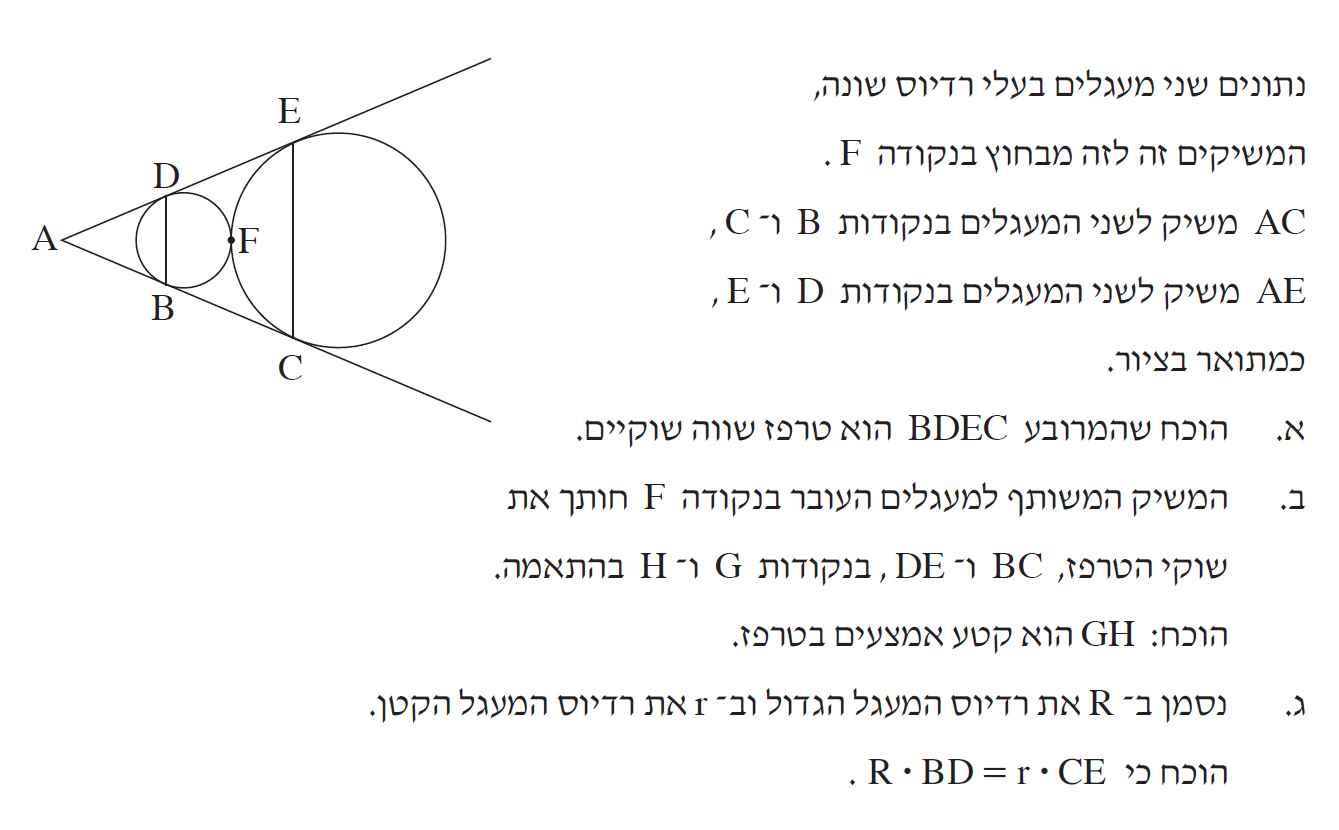
\includegraphics[width=\textwidth]{winter-2017-4}
\end{center}
\vspace{-8mm}
\textbf{סעיף א}

המשפט הרלוונטי ביותר הוא משפט
$80$
"שני משיקים למעגל היוצאים מאותה נקודה שווים זה לזה". נפעיל אותו על
$AC,AE$:
\begin{equationarray*}{rcl}
AD&=&AB=a\\
AE&=&AC=a+b\\
DE&=&BC=b\,.
\end{equationarray*}
אם נוכיח ש-%
$DB\|EC$,
המרובע
$BDEC$
יהיה טרפז לפי ההגדרה והוכחנו שהוא שווה שוקיים.

לפי הציור
$\triangle ADB\sim \triangle AEC$
וזה יכול לתרום לפתרון. המשולשים דומים כי יש להם זווית משותפת ב-%
$A$
והוכחנו ש-%
$\frac{AD}{AE}=\frac{a}{a+b}=\frac{AB}{AC}$,
כך שהמשולשים דומים לפי צ.ז.צ. המשולשים
$\triangle ADB,\triangle AEC$
שווה שוקיים, ולכן לפי משפט
$6$
"במשולש שווה שוקיים , חוצה זווית הראש, התיכון לבסיס והגובה לבסיס מתלכדים". הקו 
$c$,
חוצה הזווית 
$\angle A$,
הוא גם גובה. מכאן שבסיסי המשולשים
$DB, EC$
מאונכים שניהם לקו
$c$
ו-%
$DB\perp EC$.
\begin{center}
\selectlanguage{english}
\begin{tikzpicture}[scale=.9]
\coordinate [label=left:$A$] (A) at (0,0);
\fill (A) circle(1.5pt);
\node[circle,draw,thick] (o1) at (5.4,0) [minimum size=2.7cm] {};
\node[circle,draw,thick] (o2) at (9,0) [minimum size=4.5cm] {};
\coordinate (F) at (6.75,0);
\coordinate (B) at (tangent cs:node=o1,point={(A)},solution=1);
\coordinate (D) at (tangent cs:node=o1,point={(A)},solution=2);
\coordinate (C) at (tangent cs:node=o2,point={(A)},solution=1);
\coordinate (E) at (tangent cs:node=o2,point={(A)},solution=2);
\fill (B) node[below] {$B$} circle(1.5pt);
\fill (D) node[above] {$D$} circle(1.5pt);
\fill (F) node[above right] {$F$} circle(1.5pt);
\fill (C) node[below] {$C$} circle(1.5pt);
\fill (E) node[above] {$E$} circle(1.5pt);
\draw[thick] (A) -- ($(A) !1.2! (E)$);
\draw[thick] (A) -- ($(A) !1.2! (C)$);
\draw[thick,name path=db] (D) -- (B);
\draw[thick,name path=ec] (E) -- (C);
\draw[thick,dashed,name path=dot] (0,0) -- node[above,near end,xshift=15mm] {$c$} (12,0);
\path[name intersections={of=db and dot,by={M}}];
\path[name intersections={of=ec and dot,by={N}}];
\fill (M) circle(1.5pt);
\fill (N) circle(1.5pt);
\draw (M) rectangle +(7pt,7pt);
\draw (N) rectangle +(7pt,7pt);
\path (A) -- node[above] {$a$} (D);
\path (A) -- node[below] {$a$} (B);
\path (D) -- node[above] {$b$} (E);
\path (B) -- node[below] {$b$} (C);
\end{tikzpicture}
\end{center}

\newpage

\textbf{סעיף ב}
במבט ראשון נראה שכדאי לעבוד עם משפט 
$43$
"קטע האמצעים בטרפז מקביל לבסיסים ושווה למחצית סכומם", כאן, 
$GH=\frac{1}{2}(BD+CE)$.
תחילה עלה בדעתי שאפשר להשתמש בנוסחה לשטח של טרפז שהיא:
\[
S_{BDEC}=h\cdot\frac{1}{2}(BD+CE)\,,
\]
אבל זה לא הוביל לפתרון. אחר כך חשבתי לחפש משולשים כדי להשתמש במשפט
$14$
"קטע אמצעים במשולש מקביל לצלע השלישית ושווה למחציתה", אבל לא מצאתי משולש מתאים.

לאחר פישוט של הציור שמתי לב ש-%
$H,G$
הן נקודות הניתן להפעיל עליהן את משפט 
$80$
שכבר השתמשתי בסעיף א. 
$DH=HF=x$
ו-%
$HE=HF=y$,
ולכן
$DH=HE$.
אותה הוכחה מראה ש-%
$BG=GC$,
ו-%
$GH$
הוא קטע אמצעים של הטרפז.

\begin{center}
\selectlanguage{english}
\begin{tikzpicture}[scale=.9]
\coordinate [label=left:$A$] (A) at (0,0);
\fill (A) circle(1.5pt);
\node[circle,draw,thick] (o1) at (5.4,0) [minimum size=2.7cm] {};
\node[circle,draw,thick] (o2) at (9,0) [minimum size=4.5cm] {};
\coordinate (F) at (6.75,0);
\path[name path=gh] (6.75,-2.2) -- (6.75,2.2);
\coordinate (B) at (tangent cs:node=o1,point={(A)},solution=1);
\coordinate (D) at (tangent cs:node=o1,point={(A)},solution=2);
\coordinate (C) at (tangent cs:node=o2,point={(A)},solution=1);
\coordinate (E) at (tangent cs:node=o2,point={(A)},solution=2);
\fill (B) node[below] {$B$} circle(1.5pt);
\fill (D) node[above] {$D$} circle(1.5pt);
\fill (F) node[above right] {$F$} circle(1.5pt);
\fill (C) node[below] {$C$} circle(1.5pt);
\fill (E) node[above] {$E$} circle(1.5pt);
\draw[thick,name path=ae] (A) -- ($(A) !1.2! (E)$);
\draw[thick,name path=ac] (A) -- ($(A) !1.2! (C)$);
\draw[thick] (D) -- (B);
\draw[thick] (E) -- (C);
\path[name intersections={of=ac and gh,by={G}}];
\path[name intersections={of=ae and gh,by={H}}];
\fill (G) node[below] {$G$} circle(1.5pt);
\fill (H) node[above] {$H$} circle(1.5pt);
\draw[thick] (G) -- (H);
\path (D) -- node[above] {$x$} (H);
\path (H) -- node[above] {$y$} (E);
\path (H) -- node[right,xshift=20pt] {$x,y$} (F);
\draw[<-] (6.75,9mm) -- +(8mm,0);
\end{tikzpicture}
\end{center}

\textbf{סעיף ג}
ניתן לכתוב את הטענה שיש להוכיח כיחס:
\[
\frac{BD}{CD}=\frac{r}{R}\,.
\]
נוכיח ש-%
$\triangle BO_1D\sim\triangle CO_2E$,
כאשר 
$O_1,O_2$
הן מרכזי המעגלים. המשולשים מורכבים משני משולשים חופפים
$\triangle MO_1D, \triangle MO_1B$
ו-%
$\triangle NO_2E, \triangle NO_2C$,
כך שמספיק להוכיח דימיון של זוג משולשים קטנים. כבר הוכחנו ש-%
$DB\|EC$
והזווית בין רדיוס למשיק היא זוויות ישרה, ולכן:
\[
\angle MDO_1=90-\angle MDA=90-\angle NEA=\angle NEO_2\,.
\]
$\triangle BO_1D\sim\triangle CO_2E$
לפי ז.ז.
\begin{center}
\selectlanguage{english}
\begin{tikzpicture}[scale=.9]
\coordinate [label=left:$A$] (A) at (0,0);
\fill (A) circle(1.5pt);
\coordinate (center1) at (5.4,0);
\coordinate (center2) at (9,0);
\node[circle,draw,thick] (o1) at (center1) [minimum size=2.7cm] {};
\node[circle,draw,thick] (o2) at (center2) [minimum size=4.5cm] {};
\coordinate (F) at (6.75,0);
\path[name path=gh] (6.75,-2.2) -- (6.75,2.2);
\coordinate (B) at (tangent cs:node=o1,point={(A)},solution=1);
\coordinate (D) at (tangent cs:node=o1,point={(A)},solution=2);
\coordinate (C) at (tangent cs:node=o2,point={(A)},solution=1);
\coordinate (E) at (tangent cs:node=o2,point={(A)},solution=2);
\fill (B) node[below] {$B$} circle(1.5pt);
\fill (D) node[above] {$D$} circle(1.5pt);
\fill (C) node[below] {$C$} circle(1.5pt);
\fill (E) node[above] {$E$} circle(1.5pt);
\draw[thick,name path=ae] (A) -- ($(A) !1.2! (E)$);
\draw[thick,name path=ac] (A) -- ($(A) !1.2! (C)$);
\draw[thick,name path=db] (D) -- (B);
\draw[thick,name path=ec] (E) -- (C);
\draw[thick,dashed,name path=dot] (0,0) -- (12,0);
\fill (center1) node[above right] {$O_1$} circle(1.5pt);
\fill (center2) node[above right] {$O_2$} circle(1.5pt);
\draw[thick,dashed] (B) -- node[right] {$r$} (center1) -- node[right] {$r$} (D);
\draw[thick,dashed] (C) -- node[right] {$R$} (center2) -- node[right] {$R$} (E);
\path[name intersections={of=dot and db,by={M}}];
\fill (M) node[above left] {$M$} circle(1.5pt);
\path[name intersections={of=dot and ec,by={N}}];
\fill (N) node[above left] {$N$} circle(1.5pt);
\draw[rotate=-74] (E) rectangle +(7pt,7pt);
\draw[rotate=-74] (D) rectangle +(7pt,7pt);
\end{tikzpicture}
\end{center}

%%%%%%%%%%%%%%%%%%%%%%%%%%%%%%%%%%%%%%%%%%%%%%%%%%%%%%%%%%%%%%%%%%%

\section{קיץ תשע"ו מועד ב}

\begin{center}
\selectlanguage{english}
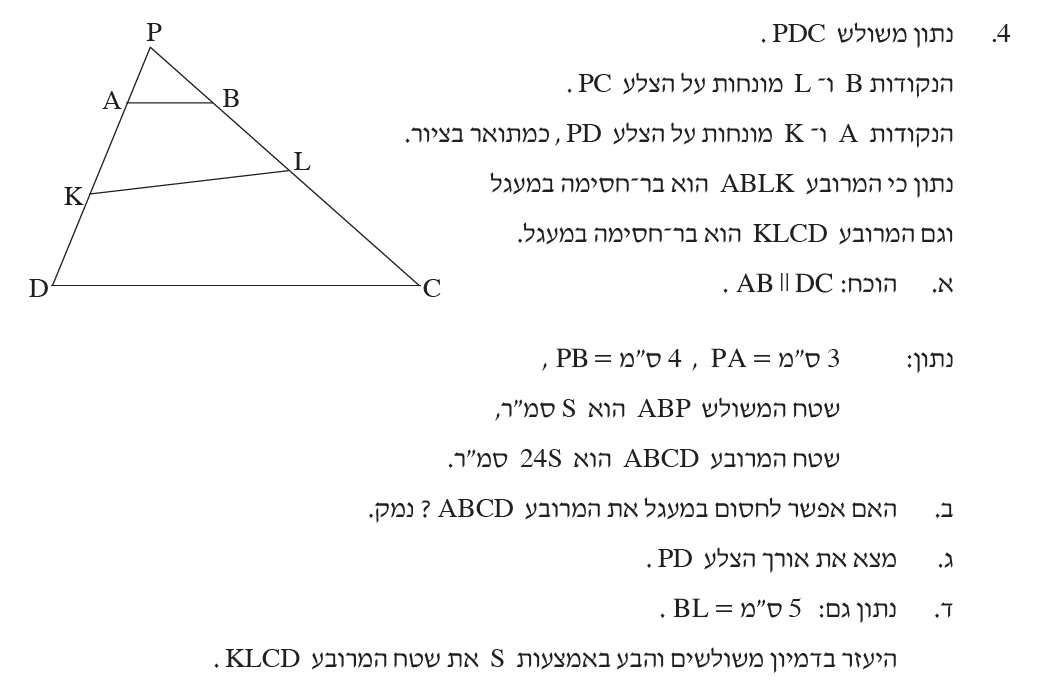
\includegraphics[width=\textwidth]{summer-2016b-4}
\end{center}
\vspace{-7mm}
\textbf{סעיף א}

שני מרובעים חסומים והמשפט המתאים הוא משפט
$56$ 
"ניתן לחסום מרובע במעגל אם ורק אם סכום זוג זוויות נגדיות שווה ל-%
$180^\circ$".
נצייר את שני המעגלים החוסמים את המרובעים, ונבחר זוג זוויות נגדיות, למשל,
$\angle LKA,\angle ABL$,
במרובע
$ABLK$.
נסמן
$\angle LKA=\alpha$
ונשתמש בקיצור
$\alpha'=180^\circ-\alpha$
עבור הזווית הנגדית
$\angle ABL$.
לפי זוויות משלימות בנקודה
$B$,
$\angle ABP=\alpha$,
ובנקודה
$K$,
$\angle LKD=\alpha'$.
נפעיל שוב את משפט
$56$
כדי להסיק ש-%
$\angle LCD=\alpha$.
מכאן ש-%
$AB\|DC$
לפי זוויות מתאימות.
\vspace{-1mm}
\begin{center}
\selectlanguage{english}
\begin{tikzpicture}
%\clip (-1,-1.7) rectangle +(5,7.2);
\coordinate [label=left:$D$] (D) at (0,0);
\coordinate [label=right:$C$] (C) at (4,0);
\coordinate [label=above:$P$] (P) at (1.5,5);
\coordinate (K) at ($(D)!.25!(P)$);
\coordinate (L) at ($(C)!.35!(P)$);
\coordinate (A) at ($(D)!.75!(P)$);
\draw[thick,name path=pd] (P) -- (D);
\draw[thick,name path=pc] (P) -- (C);
\path[name path=ab] (A) -- +(2,0);
\path[name intersections={of=ab and pc,by={B}}];
\draw[thick] (D) -- (C);
\draw[thick] (K) -- (L);
\draw[thick] (A) -- (B);
\tkzCircumCenter(A,B,L)\tkzGetPoint{O1}
\tkzDrawCircle[dotted,name path=circ1](O1,A)
\tkzCircumCenter(K,L,C)\tkzGetPoint{O2}
\tkzDrawCircle[dotted,name path=circ2](O2,L)
\fill (P) circle(1.5pt);
\fill (C) node[above left,xshift=-2pt] {$\alpha$} circle(1.5pt);
\fill (D) node[above right,xshift=2pt] {$\beta$} circle(1.5pt);
\fill (K) node[left,xshift=-6pt] {$K$} node[above right,xshift=2pt] {$\alpha$} node[below right,xshift=0pt,yshift=4pt] {$\alpha'$}  circle(1.5pt);
\fill (L) node[right,xshift=6pt] {$L$} node[left,xshift=-4pt,yshift=4pt] {$\beta$} node[below left,xshift=2pt,yshift=-2pt] {$\beta'$} circle(1.5pt);
\fill (A) node[left,xshift=-6pt] {$A$} node[below right,xshift=-4pt] {$\beta'$}  node[above right,xshift=0pt] {$\beta$} circle(1.5pt);
\fill (B) node[below left,xshift=2pt] {$\alpha'$} node[above left,xshift=-3pt] {$\alpha$} node[right,xshift=6pt] {$B$} circle(1.5pt);
\end{tikzpicture}
\end{center}

\textbf{סעיף ב}

כדי להפעיל שוב את משפט
$56$
נצטרך להוכיח שהזוויות הנגדיות במרובע
$ABCD$
מקיימות
$\angle BAD+\angle BCD=180, \angle ADC+\angle ABC=180$.
נסמן
$\angle ADC=\beta$.

הוכחנו ש-%
$AB\|DC$,
ולפי זוויות חד-מתאימות בנקודות
$A,D$
ו-%
$B,C$,
וזוויות משלימות בנקודות
$A,B$,
נקבל
$\angle PAB=\angle ADC=\beta$,
$\angle PBA=\angle BCD=\alpha$.

אם המרובע 
$ABCD$
בר-חסימה,
$\alpha'+\beta=180-\alpha+\beta=180$,
כך ש-%
$\alpha=\beta$,
אבל נתון ש-%
$PA\neq PB$.
המסקנה היא שלא ניתן לחסום את המרובע
$ABCD$.

\textbf{סעיף ג}

$\triangle PAB \sim \triangle PDC$
לפי ז.ז. אולם, זה לא עוזר: אמנם נתון היחס בין
$PA,PB$,
אבל יש שני זוגות של נעלמים
$PD,PC$
ו-%
$AB,DC$.
מה שכן ניתן הוא שטחים של שני המושלים, ולפי משפט
$100$
ז "יחס הצלעות הוא השורש של יחס השטחים", נכול לחשב את יחס הצלעות:
\[
\frac{PA}{PD}=\sqrt{\frac{S_{ABP}}{S_{PDC}}} = \sqrt{\frac{S_{ABP}}{S_{ABP} + S_{ABCD}}}=\sqrt{\frac{S}{S+24S}}=\frac{1}{5}\,.
\]
האורך של 
$PD$
הוא
$5\cdot PA=15$.

\textbf{סעיף ד}

מהזוויות שחישבנו ורשמנו באיור,
$\triangle PBA \sim \triangle PKL$
לפי ז.ז. יחס השטחים מתקבל מיחס אורכי הצלעות הנתונים ושחישבנו:
\[
\renewcommand{\arraystretch}{1.8}
\begin{array}{l}
\displaystyle\frac{S_{PBA}}{S_{PKL}}=\left(\frac{PA}{PL}\right)^2=\left(\frac{3}{9}\right)^2=\frac{1}{9}\\
S_{KLCD}=S_{PDC}-S_{PKL}=25S-9S=16S\,.
\end{array}
\]
\vspace{-2mm}
\begin{center}
\selectlanguage{english}
\begin{tikzpicture}%[scale=1.2]
\coordinate [label=left:$D$] (D) at (0,0);
\coordinate [label=right:$C$] (C) at (4,0);
\coordinate [label=above:$P$] (P) at (1.5,5);
\coordinate (K) at ($(D)!.25!(P)$);
\coordinate (L) at ($(C)!.35!(P)$);
\coordinate (A) at ($(D)!.75!(P)$);
\draw[thick,name path=pd] (P) -- (D);
\draw[thick,name path=pc] (P) -- (C);
\path[name path=ab] (A) -- +(2,0);
\path[name intersections={of=ab and pc,by={B}}];
\draw[thick] (D) -- (C);
\draw[thick] (K) -- (L);
\draw[thick] (A) -- (B);
\fill (P) circle(1.5pt);
\fill (C) circle(1.5pt);
\fill (D) circle(1.5pt);
\fill (K) node[left,xshift=-6pt] {$K$} node[above right] {$\alpha$} circle(1.5pt);
\fill (L) node[right,xshift=6pt] {$L$} node[left,xshift=-4pt,yshift=4pt] {$\beta$}  circle(1.5pt);
\fill (A) node[left,xshift=-6pt] {$A$} node[above right] {$\beta$} circle(1.5pt);
\fill (B) node[above left,xshift=-3pt] {$\alpha$} node[right,xshift=6pt] {$B$} circle(1.5pt);
\path (B) -- node[right] {$4$} (P);
\path (L) -- node[right] {$5$} (B);
\path (A) -- node[left] {$3$} (P);
\end{tikzpicture}
\end{center}


%%%%%%%%%%%%%%%%%%%%%%%%%%%%%%%%%%%%%%%%%%%%%%%%%%%%%%%%%%%%%%%%%%%


\newpage

\section{קיץ תשע"ו מועד א}

\begin{center}
\selectlanguage{english}
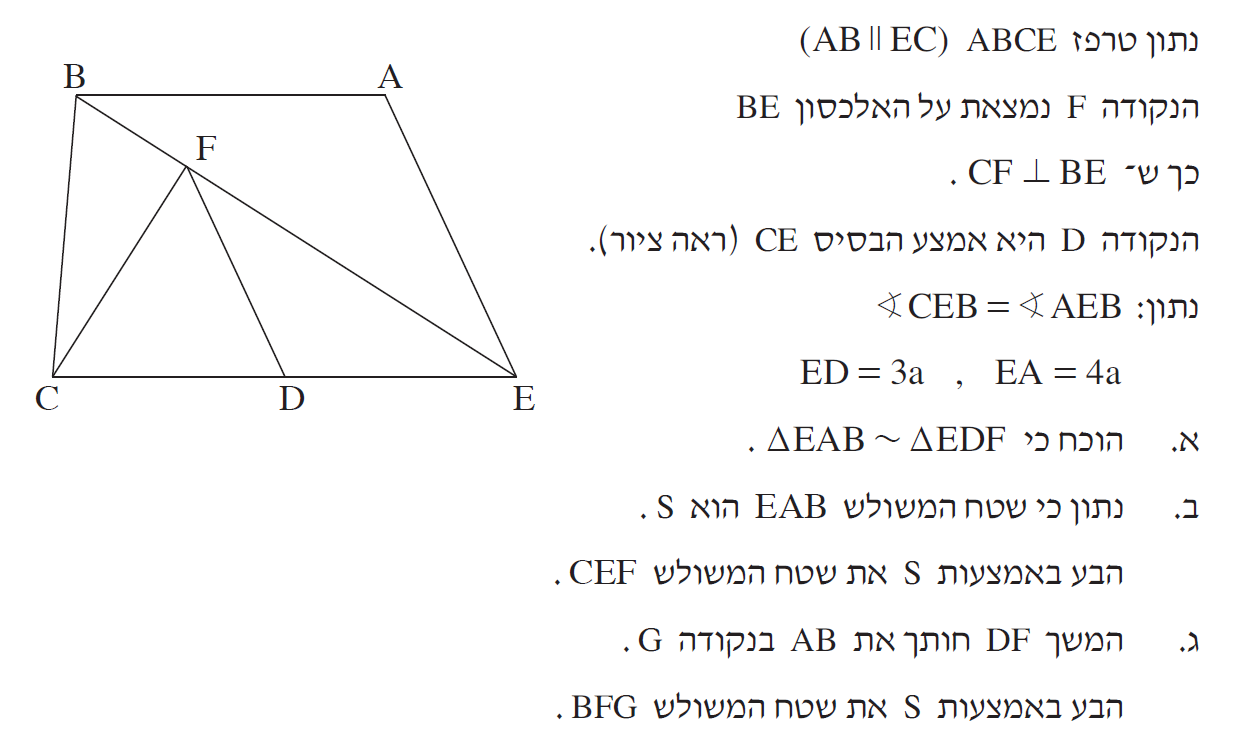
\includegraphics[width=\textwidth]{summer-2016a-4}
\end{center}

\textbf{סעיף א}

נסמן את הזוויות
$\angle AEB=\angle CEB=\alpha$
ונמסן את האורכים הנתונים. כעת קופץ לעין משפט
$86$
"במשולש ישר זווית התיכון ליתר שווה למחצית היתר", ולכן
$DF=CD=DE$,
ו-%
$\triangle EDF$
שווה שוקיים, 
$\angle DFE=\alpha$.
כמו כן, נתון ש-%
$AB\|EC$,
כך ש-%
$\angle ABE=\alpha$
לפי זוויות מתחלפות עם
$\angle CEB$. 
לפי ז.ז.
$\triangle EDF \sim \triangle EAB$.
\vspace{-10mm}
\begin{center}
\selectlanguage{english}
\begin{tikzpicture}[scale=.9]
\coordinate [label=above right:$A$] (A) at (6.5,4.5);
\coordinate [label=above left:$B$] (B) at (.5,4.5);
\coordinate [label=below right:$E$] (E) at (10,0);
\coordinate [label=below left:$C$] (C) at (0,0);
\coordinate [label=below:$D$] (D) at (5,0);
\coordinate [label=above right:$F$] (F) at ($(B)!(C)!(E)$);
\fill (A) circle(1.5pt);
\fill (B) node[below right,xshift=18pt] {$\alpha$} circle(1.5pt);
\fill (C) circle(1.5pt);
\fill (D) circle(1.5pt);
\fill (E) node[above left,xshift=-18pt,yshift=-1pt] {$\alpha$} node[above left,xshift=-14pt,yshift=12pt] {$\alpha$} circle(1.5pt);
\fill (F) node[below right,xshift=14pt,yshift=-11pt] {$\alpha$} circle(1.5pt);
\draw[thick] (A) -- (B) -- (C) -- (E) -- cycle;
\draw[thick] (B) -- (E);
\draw[thick] (C) -- (F) -- (D);
\path[name path=cf] (C) -- ($ (C) ! 1.8 ! (F) $);
\path[name path=ab] (A) -- (B);
%\path [name intersections={of=cf and ab,by={G}}];
%\fill (G) node[above] {$G$} circle(1.5pt);
%\draw[thick] (F) -- (G);
\draw[rotate=-114] (F) rectangle +(7pt,7pt);
\path (C) -- node[below,yshift=-2pt] {$3a$} (D);
\path (A) -- node[right,xshift=2pt] {$4a$} (E);
\path (D) -- node[below,yshift=-2pt] {$3a$} (E);
\path (F) -- node[left,yshift=0pt] {$3a$} (D);
\draw[thick,dashed] (F) -- ($ (C)!(F)!(D) $) coordinate(H);
\draw (H) rectangle +(7pt,7pt);
\end{tikzpicture}
\end{center}


\textbf{סעיף ב}

כדי לחשב את השטח של 
$\triangle CEF$
יש לנו בסיס
$CE$
ונבנה גובה מ-%
$F$
ל-%
$CE$.
חדי עין ישימו לב גובה זה משותף לשני המשולשים
$\triangle CFD,\triangle DFE$.
הבסיסים
$CD=DE=3a$
שווים, ולכן השטחים של שני המשולים שווים.

בסעיף א הוכחנו ש-%
$\triangle CEB\sim AEB$,
לפי משפט
$100$%
ז "יחס השטחים שווה לריבוע יחס הדמיון":
\[
\renewcommand*{\arraystretch}{1.5}
\begin{array}{l}
\displaystyle\frac{S_{DFE}}{S_{EAB}}= \left(\frac{DE}{AE}\right)^2= \left(\frac{3a}{4a}\right)^2=\frac{9}{16}\\
S_{CEF} = S_{CFD}+S_{DFE}=2 \, S_{DFE}= \frac{9}{8}\, S\,.
\end{array}
\]

\textbf{סעיף ג}

אנחנו צריכים לחשב את האורך של צלע של
$\triangle BFG$
כדי לחשב את יחס השטחים. כבר הראינו ש-%
$\angle ABE = \angle BEC=\alpha$
ו-%
$\angle BFG = \angle DFE=\alpha$
הן זוויות קודקודיות. לכן
$\triangle BFG \sim \triangle DFE$
לפי ז.ז. הזווית
$\angle AGD=2\alpha$
לפי משפט
$13$
"זווית חיצונית למשולש שווה לסכום שתי הזוויות הפנימיות שאינן צמודות לה". המרובע
$AGDE$
הוא מקבילית לפי משפט
$29$
"מרובע שבו כל זוג זוויות נגדיות שוות הוא מקבילית". 
$GD=GF+FD$
וכעת ניתן לחשב את
$GF$:
\[
GF=GD-DF=AE-DF=4a-3a=a\,,
\]
ולהשתמש שוב במשפט
$101$%
ז:
\begin{equationarray*}{rcl}
\frac{S_{BFG}}{S_{DFE}}&=&\left(\frac{a}{3a}\right)^2=\frac{1}{9}\\\\
S_{BFG}&=&\frac{1}{9}S_{DFE}=\frac{1}{9}\cdot\frac{1}{2}S_{CEF}=\frac{1}{(9\cdot 2)}\frac{9}{8}S=\frac{1}{16}S\,.
\end{equationarray*}

\vspace{-15mm}

\begin{center}
\selectlanguage{english}
\begin{tikzpicture}[scale=.9]
\coordinate [label=above right:$A$] (A) at (6.5,4.5);
\coordinate [label=above left:$B$] (B) at (.5,4.5);
\coordinate [label=below right:$E$] (E) at (10,0);
\coordinate [label=below left:$C$] (C) at (0,0);
\coordinate [label=below:$D$] (D) at (5,0);
\coordinate (F) at ($(B)!(C)!(E)$);
\fill (A)  node[below left] {$180-2\alpha$}circle(1.5pt);
\fill (B) node[below left,xshift=-8pt,yshift=-8pt] {$\alpha$} circle(1.5pt);
\draw[<-] (1.1,4.4) -- +(-155:26pt);
\draw[<-] (1.4,4.2) -- +(-170:33pt);
\fill (C) circle(1.5pt);
\fill (D) node[above left,xshift=-4pt] {$2\alpha$} node[above right,xshift=-4pt] {$180-2\alpha$} circle(1.5pt);
\fill (E) node[above left,xshift=-18pt,yshift=-1pt] {$\alpha$} node[above left,xshift=-14pt,yshift=12pt] {$\alpha$}  circle(1.5pt);
\fill (F) node[below left,xshift=4pt,yshift=-4pt] {$F$} node[below right,xshift=16pt,yshift=-12pt] {$\alpha$} circle(1.5pt);
\draw[thick] (A) -- (B) -- (C) -- (E) -- cycle;
\draw[thick] (B) -- (E);
\draw (D) -- (F);
%\draw[thick] (F) -- (C);
\path[name path=df] (D) -- ($ (D) ! 1.8 ! (F) $);
\path[name path=ab] (A) -- (B);
\path [name intersections={of=df and ab,by={G}}];
\fill (G) node[above] {$G$} node[below right,xshift=8pt] {$2\alpha$} circle(1.5pt);
\draw[thick] (F) -- (G);
%\draw[rotate=-114] (F) rectangle +(7pt,7pt);
%\path (C) -- node[below,yshift=-2pt] {$3a$} (D);
\path (A) -- node[right,xshift=2pt] {$4a$} (E);
\path (D) -- node[below,yshift=-2pt] {$3a$} (E);
\path (F) -- node[left,yshift=0pt] {$3a$} (D);
%\draw[thick,dashed] (F) -- ($ (C)!(F)!(D) $) coordinate(H);
%\draw (H) rectangle +(7pt,7pt);
\end{tikzpicture}
\end{center}

%%%%%%%%%%%%%%%%%%%%%%%%%%%%%%%%%%%%%%%%%%%%%%%%%%%%%%%%%%%%%%%%%%%

\newpage


\section{חורף תשע"ו}

\begin{center}
\selectlanguage{english}
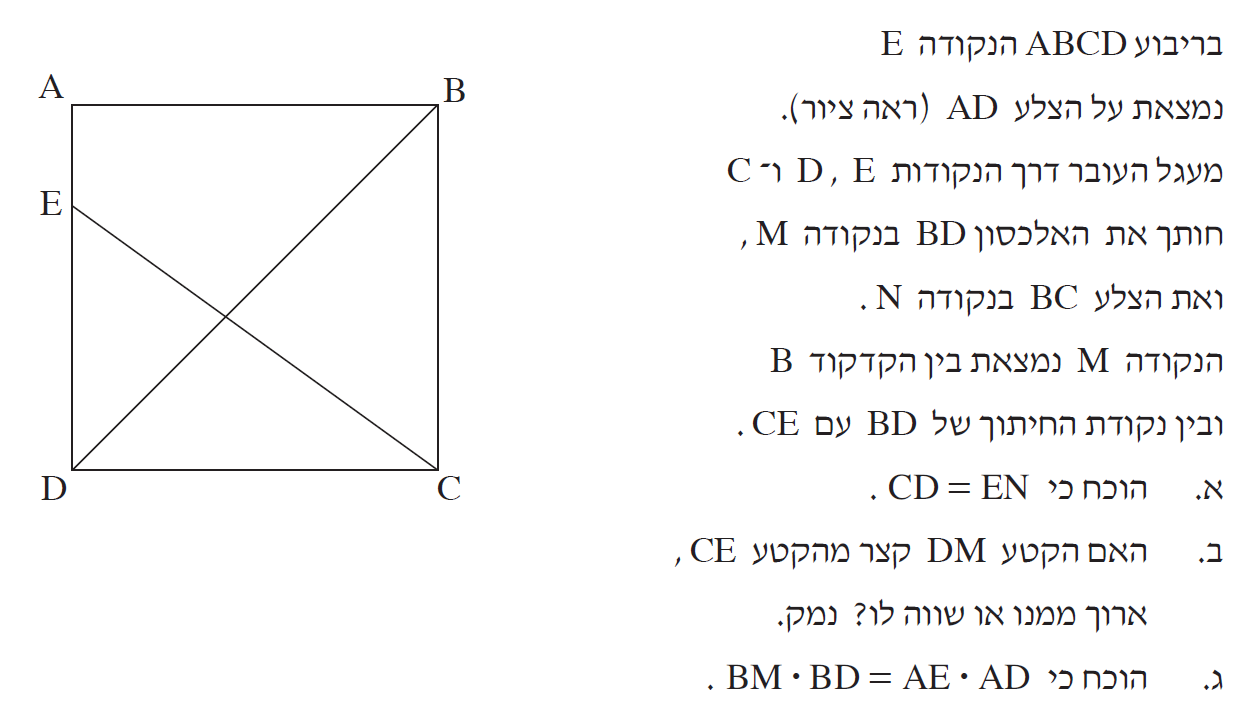
\includegraphics[width=.9\textwidth]{winter-2016-4}
\end{center}

\vspace{-2mm}

\textbf{סעיף א}

קשה להבין את השאלה אלא אם מציירים ציור חדש עם הנקודות 
$M,N$
והקו
$EN$.
המעגל מוגדר כך שהוא עובר דרך הנקודות
$C,D,E$,
ונתון גם שהנקודה
$N$
נמצאת על המעגל. מכאן ש-%
$ENDC$
הוא מרובע הסום במעגל. נשתמש במשפט 
$56$
"ניתן לחסום מרובע במעגל אם ורק אם סכום זוג זוויות נגדיות שווה ל-%
$180^\circ$".
$ABCD$
הוא ריבוע כך ש-%
$\angle ADC=\angle EDC=90^\circ$,
$\angle BCD=\angle NCD=90^\circ$.
לפי המשפט:
\[
\angle ENC=180-\angle EDC=90,\quad \angle NED=180-\angle NCD=90\,.
\]
מרובע שכל הזוויות שלו ישרות הוא מלבן ו-%
$CD=EN$.

\begin{center}
\selectlanguage{english}
\begin{tikzpicture}[scale=.85]
\coordinate [label=above left:$A$] (A) at (0,5);
\coordinate [label=above right:$B$] (B) at (5,5);
\coordinate [label=below right:$C$] (C) at (5,0);
\coordinate [label=below left:$D$] (D) at (0,0);
\coordinate [label=left:$E$] (E) at (0,3.5);
\draw[thick] (A) -- (B) -- (C) -- (D) -- cycle;
\draw[thick,name path=db] (D) -- (B);
\draw[thick,name path=ce] (C) -- (E);
\fill (A) circle(1.5pt);
\fill (B) circle(1.5pt);
\fill (C) circle(1.5pt);
\fill (D) circle(1.5pt);
\fill (E) circle(1.5pt);
\tkzCircumCenter(C,D,E)\tkzGetPoint{O}
\tkzDrawCircle[thick,name path=circ](O,C)
\path [name intersections={of=db and ce,by={F}}];
%\fill (F) node[above,yshift=4pt] {$F$} circle(1.5pt);
\path [name intersections={of=circ and db,by={M}}];
\fill (M) node[left,xshift=-4pt] {$M$} circle(1.5pt);
\path[name path=bc] (B) -- (C);
\path [name intersections={of=circ and bc,by={N}}];
\fill (N) node[right] {$N$} circle(1.5pt);
\draw[thick,dashed] (E) -- (N);
\draw[rotate=0] (D) rectangle +(7pt,7pt);
\draw[rotate=90] (C) rectangle +(7pt,7pt);
\end{tikzpicture}
\end{center}
הוכחה אחרת משתמשת במשפט
$74$
"זווית היקפית בת 
$90^\circ$
נשענת על קוטר". הנקודות
$C,D,E,N$
נמצאות על מעגל, 
$\angle EDC=90^\circ$,
כך ש-%
$EC$
הוא קוטר לפי משפט
$74$
"זווית היקפית בת
$90^\circ$
נשענת על קוטר". לפי המשפט ההפוך
$(73)$
$\angle ENC=90^\circ$.
כדי להשלים את סכום הזוויות במרובע ל-%
$360^\circ$,
$\angle NED$
חייב להיות 
$90^\circ$
ו-%
$ENDC$
הוא מלבן.


\textbf{סעיף ב}

בזבזתי הרבה זמן בנסיונות לפתור סעיף זה כי חשבתי להשוות אורכים לפי משולשים דומים או משפט פיתגורס. לבסוף נזכרתי במשפט
$66$
"במעגל, אם מרחקו של מיתר ממרכז המעגל קטן יותר ממרחקו של מיתר אחר, אז מיתר זה ארוך יותר מהמיתר האחר". בהוכחה השנייה לסעיף א ראינו ש-%
$EC$
הוא קוטר, וקוטר הוא מיתר הקרוב ביותר למרכז המעקל )עובר דרכו( ולכן הוא ארוך יותר מכל מיתר שאינו קוטר. מה שנשאר לעשות הוא להוכיח ש-%
$DM$
אינו קוטר.

נתון שהנקודה
$M$
נמצאת בין 
$B$
לבין נקודת החיתוך המסומן ב-%
$F$.
נתון גם ש-%
$E$
נמצאת על
$AD$
ונניח שהכוונה היא ש-%
$E$
שונה מנקודות הקצה
$A,D$.
הוכחנו ש-%
$EN\|AB$
ולכן אם 
$E$
שונה מ-%
$A$
גם
$N$
שונה מ-%
$B$,
ו-%
$M$
אינה מתלכדת עם
$N$.
\vspace{-4mm}

\begin{center}
\selectlanguage{english}
\begin{tikzpicture}[scale=.85]
\coordinate (A) at (0,5);
\coordinate (B) at (5,5);
\coordinate [label=below right:$C$] (C) at (5,0);
\coordinate [label=below left:$D$] (D) at (0,0);
\coordinate [label=left:$E$] (E) at (0,3.5);
\draw[thick,name path=db] (D) -- (B);
\draw[thick,name path=ce] (C) -- (E);
\fill (A) node[above left] {$A$} circle(1.5pt);
\fill (B) node[above right] {$B$} circle(1.5pt);
\fill (C) circle(1.5pt);
\fill (D) circle(1.5pt);
\fill (E) circle(1.5pt);
\tkzCircumCenter(C,D,E)\tkzGetPoint{O}
\tkzDrawCircle[thick,name path=circ](O,C)
\path [name intersections={of=db and ce,by={F}}];
\fill (F) node[above,yshift=4pt] {$F$} circle(1.5pt);
\path [name intersections={of=circ and db,by={M}}];
\fill (M) node[left,xshift=-4pt] {$M$} circle(1.5pt);
\path[name path=bc] (B) -- (C);
\path [name intersections={of=circ and bc,by={N}}];
\fill (N) node[right] {$N$} circle(1.5pt);
\draw[thick,dashed] (D) -- (N);
\draw[rotate=0] (D) rectangle +(7pt,7pt);
\draw[rotate=90] (C) rectangle +(7pt,7pt);
\fill (O) node[below,yshift=-4pt] {$O$} circle(1.5pt);
\draw[thick] (B) -- (A) -- (D) -- (C) -- (N) -- (B) -- (D);
\draw[thick,dashed] (E) -- (N);
\end{tikzpicture}
\end{center}

%\newpage

\vspace{-30mm}

\textbf{סעיף ג}

הנטייה הראשונה היא להשתמש במשפט תאלס, אבל משפט זה מנוסח כחילוק ולא ככפל על קטעים של אותו קן. המשפט שמנוסח בכפל הוא משפט
$102$
"אם מנקודה מחוץ למעגל יוצאים שני חותכים, אז מכפלת חותך אחד בחלקו החיצוני שווה למכפלת החותך השני בחלקו החיצוני". נשתמש במשפט זה עבור החותכים
$BC,BD$
היוצאים מנקודה
$B$
ונקבל
$BM\cdot BD = BN \cdot BC$.

$AD=BC$
כי הם צלעות בריבוע 
$ABCD$,
ו-%
$ED=NC$
כי הם צעלות של
$ENCD$
שהוכחנו בסעיף א שהוא מלבן. מכאן:
\[
BM\cdot BD =  BN \cdot BC = (BC-NC)\cdot BD = (AD-ED) \cdot AD = AE\cdot AD\,.
\]


%%%%%%%%%%%%%%%%%%%%%%%%%%%%%%%%%%%%%%%%%%%%%%%%%%%%%%%%%%%%%%%%%%%

\newpage


\section{קיץ תשע"ה מועד ב}

\begin{center}
\selectlanguage{english}
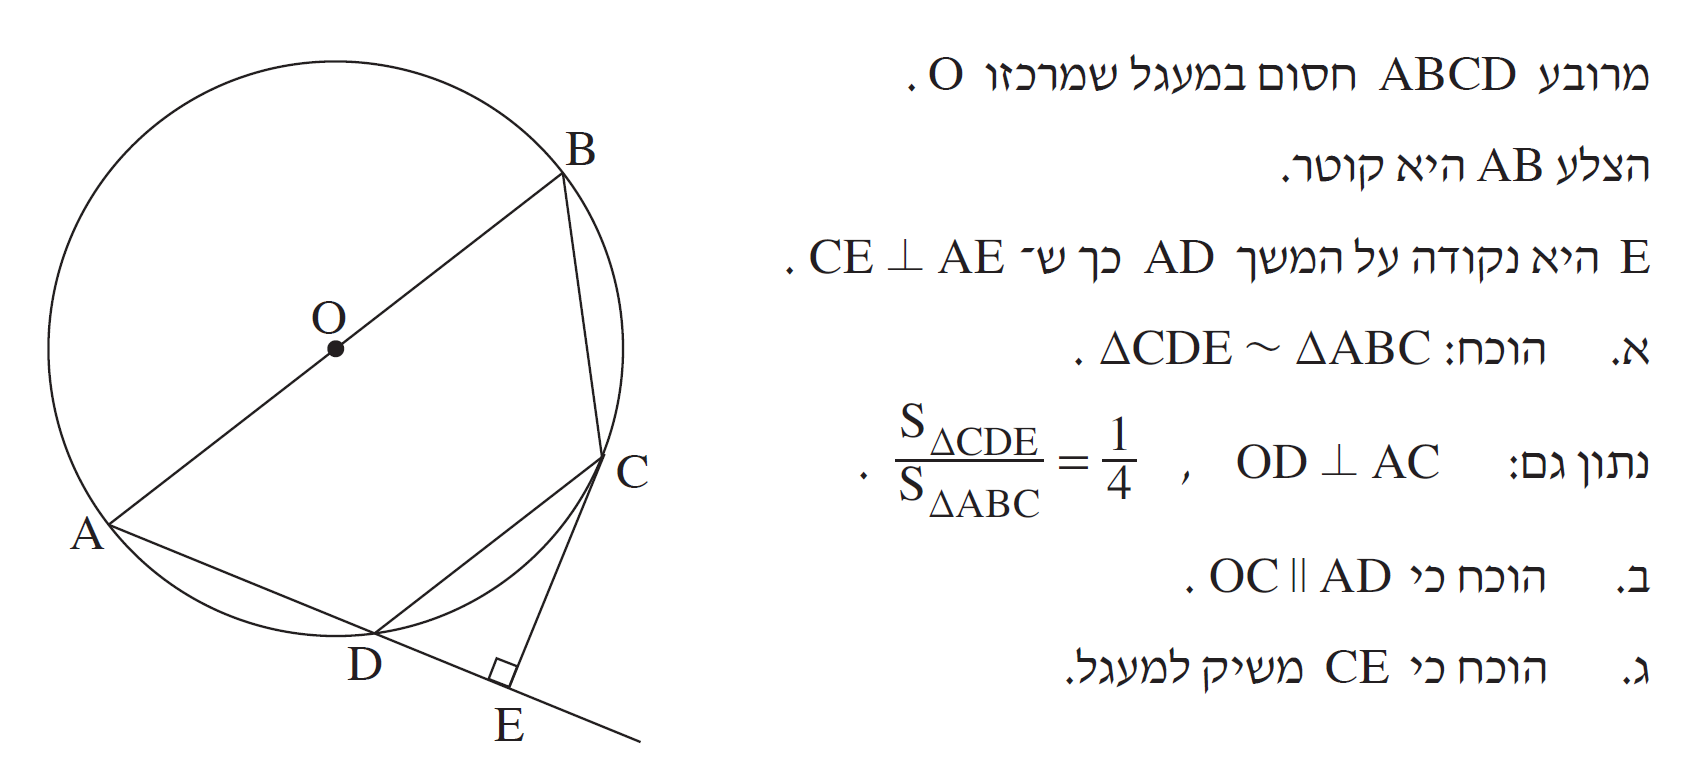
\includegraphics[width=\textwidth]{summer-2015b-4}
\end{center}

\textbf{סעיף א}

מרובע חסום במעגל מכוון למשפט
$56$
"ניתן לחסום מרובע במעגל אם ורק אם סכום זוג זוויות נגדיות שווה ל-%
$180^\circ$". 
נתון גם שצלע שלו הוא קוטר והמשפט ררלוונטי הוא
$73$
"זווית היקפית הנשענת על קוטר היא זווית ישרה 
$(90^\circ)$".
כדי לקבל את המשלוש
$\triangle ABC$,
נצייר את הקו
$AC$

ו-%
$\angle ACB=90^\circ$
כי הוא נשען על קוטר. 

נסמן זוויות לפי משפט
$(56)$:
$\angle ABC=\alpha$,
$\angle BAC=180-\alpha=\alpha'$.
לפי זוויות משלימות בנקודה
$D$,
$\angle CDE=180-\alpha'=\alpha=\angle ABC$,
ו-%
$\triangle CDE \sim \triangle ABC$
לפי ז.ז.


\begin{center}
\selectlanguage{english}
\begin{tikzpicture}[scale=.9]
\coordinate [label=above:$O$] (O) at (0,0);
\coordinate [label=below left:$A$] (A) at (-2,-2);
\fill (O) circle(1.5pt);
\fill (A) circle(1.5pt);
\node [draw,thick,circle through=(A),name path=circ] (circle) at (O) {};
\path [name path=diam] (A) -- +(45:6);
\path [name intersections={of=circ and diam,by={B}}];
\fill (B) node[above right] {$B$} node[below,xshift=-3pt,yshift=-6pt] {$\alpha$} circle(1.5pt);
\draw[thick] (A) -- (B);
\draw [thick,name path=ad] (A) -- +(-15:5);
\path [name intersections={of=circ and ad,by={dummy1,D}}];
\fill (D) node[below] {$D$} node[right,xshift=10pt,yshift=1pt] {$\alpha?$} node[above,xshift=0pt,yshift=0pt] {$\alpha'$} circle(1.5pt);
\path [thick,name path=dc] (D) -- +(45:4);
\path [name intersections={of=circ and dc,by={dummy2,C}}];
\fill (C) node[right] {$C$} circle(1.5pt);
\draw [thick] (D) -- (C) -- (B);
\coordinate (E) at ($(A)!(C)!(D)$);
\fill (E)  node[below] {$E$} circle(1.5pt);
\draw[thick] (C) -- (E);
\draw[rotate=76] (E) rectangle +(5pt,5pt);
\draw[thick,dashed] (A) -- (C);
\draw[rotate=108] (C) rectangle +(5pt,5pt);
\end{tikzpicture}
\end{center}

\textbf{סעיף ב}

בציור נראה שהמרובע
$AODC$
הוא מקבילית, ואם כן, 
$OC\|AD$.
נתון גם ש-%
$OD\perp AC$,
כך שאם המרובע הוא מקבילית, הוא גם מעוין לפי משפט
$36$
"מקבילית שבה האלכסונים מאונכים זה לזה היא מעוין". למעשה לא צריך להשתמש במשפט
$36$
כדי להוכיח שהמקבילית היא מעוין כי 
$OA=OC=r$.
מכאן שסביר יותר שהנתון
$OD\perp AC$
יעזור להוכיח ש-%
$AODC$
הוא מקבילית.

כעת נפנה לנתון על יחס השטחים של המשולשים. לפי משפט
$100$%
ז "יחס השטחים שווה לריבוע יחס הדמיון", היחס הצלעות במשולשים הדומים הוא
$\sqrt{\frac{1}{4}}=\frac{1}{2}$.
מכאן ש-%
$CD=\frac{1}{2}AB=\frac{1}{2}\cdot 2r=r$.
אם נוכיח ש-%
$AD=r$
יהיה לנו את המקבילית )מעוין( שנחוץ כדי להוכיח ש-%
$OC\|AD$.

נחזור לנתון
$OD\perp AC$.
הוכחנו ש-%
$\triangle OCD$
הוא שווה שוקיים )למעשה הוא שווה צלעות(, כך ש-%
$CA$
הוא גובה ל-%
$OD$,
ולפי משפט
$6$
"במשולש שווה שוקיים , חוצה זווית הראש, התיכון לבסיס והגובה לבסיס מתלכדים", ולכן
$OF=FD=\frac{r}{2}$
ו-%
$\triangle OCF\cong\triangle DCF$.\footnote{%
החפיפה נובעת ממשפט 
$20$
"משפט חפיפה שתי צלעות והזווית שמול הצלע הגדולה מבין השתיים" לאחר שנטען שהזווית הישרה גדולה יותר מהזוויות האחרות. בספרי גיאומטריה משתמשים במשפט זה כך: שני משלושים ישר זווית חופפים עם היתר וצלע אחר שווים.%
}
אותה הוכחה מראה ש-%
$\triangle OAF\cong \triangle OCF$
ו-%
$\triangle DAF\cong \triangle OAF$.
מכאן ש-%
$AD=OA=r$.
\begin{center}
\selectlanguage{english}
\begin{tikzpicture}[scale=.9]
\coordinate [label=above:$O$] (O) at (0,0);
\coordinate [label=below left:$A$] (A) at (-2,-2);
\fill (O) circle(1.5pt);
\fill (A) circle(1.5pt);
\node [draw,thick,circle through=(A),name path=circ] (circle) at (O) {};
\path [name path=diam] (A) -- +(45:6);
\path [name intersections={of=circ and diam,by={B}}];
\fill (B) node[above right] {$B$} circle(1.5pt);
\draw[thick] (A) -- (B);
\draw [thick,name path=ad] (A) -- +(-15:5);
\path [name intersections={of=circ and ad,by={dummy1,D}}];
\fill (D) node[below] {$D$} circle(1.5pt);
\path [thick,name path=dc] (D) -- +(45:4);
\path [name intersections={of=circ and dc,by={dummy2,C}}];
\fill (C) node[right] {$C$} circle(1.5pt);
\draw [thick] (D) -- node[above] {$r$} (C) -- (B);
\coordinate (E) at ($(A)!(C)!(D)$);
\fill (E)  node[below] {$E$} circle(1.5pt);
\draw[thick] (C) -- (E);
\draw[rotate=76] (E) rectangle +(5pt,5pt);
\draw[thick,dashed,name path=ac] (A) -- (C);
\draw[rotate=107] (C) rectangle +(5pt,5pt);
\draw[thick,dashed,name path=od] (D) -- node[left,near end,yshift=-2pt] {$r/2$} node[left,near start,yshift=-2pt] {$r/2$} (O) -- node[above] {$r$} (C);
\path [name intersections={of=ac and od,by={F}}];
\fill (F) node[above right] {$F$} circle(1.5pt);
\draw[rotate=107] (F) rectangle +(5pt,5pt);
\path (A) -- node[above] {$r$} (O) -- node[above] {$r$} (B);
\path (A) -- node[below,yshift=-14pt] {$r?$} (D);
\draw[<-] ($(A) !.5 ! (D) $) -- +(0,-16pt);
\end{tikzpicture}
\end{center}
בפתרונות אחרים שראיתי, משתמשים בעובדה ש-%
$\triangle OCD$
הוא שווה צלעות שהזוויות שלו הן
$60^\circ$.
לא מצאתי שערך זה נחוץ כדי להוכיח את הטענה.

\textbf{סעיף ג}

המשפט היחיד שהמסקנה שלו היא שקו הוא משיק הוא משפט
$78$
"ישר המאונך לרדיוס בקצהו הוא משיק למעגל", כאן
$CE\perp OC$.
כאן כן נשתמש בעובדה ש-%
$\triangle OCD,\triangle OAD$
הם שווה צלעות ו-%
$\angle OCD=\angle OAD=60^\circ$.
בסעיף א הוכחנו ש-%
$\triangle ABC\sim \triangle CDE$,
כך ש-%
$\angle CAB = \angle ECD$.
בסעיף ב הוכחנו ש-%
$AC$
הוא חוצה זווית של
$\angle OAD$.
מכאן ש-%
\[
\angle ECO = \angle ECD + \angle OCD = \angle CAB + 60^\circ = \frac{1}{2}\angle OAD + 60^\circ=\frac{1}{2}\cdot 60^\circ + 60^\circ = 90^\circ\,.
\]


%%%%%%%%%%%%%%%%%%%%%%%%%%%%%%%%%%%%%%%%%%%%%%%%%%%%%%%%%%%%%%%%%%%
\newpage


\section{קיץ תשע"ה מועד א}

\begin{center}
\selectlanguage{english}
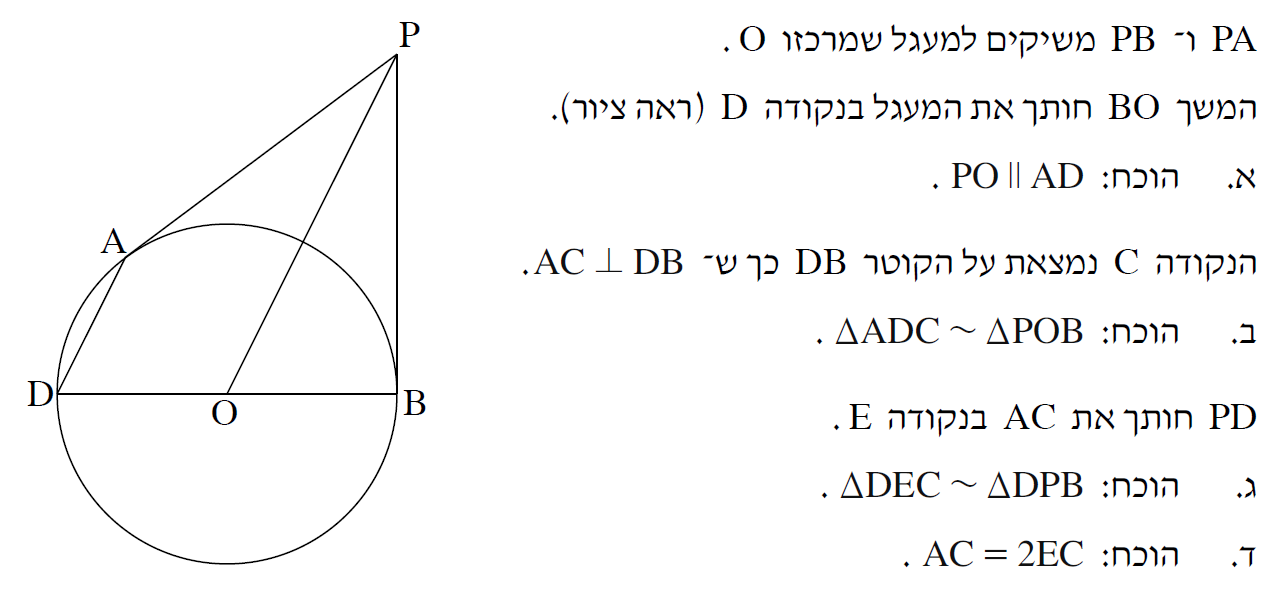
\includegraphics[width=\textwidth]{summer-2015a-4}
\end{center}

\textbf{סעיף א}
כאשר יש שני משיקים וקו מהנקודת החיתוך של המשיקים למרכז המעגל המשפטים האלה עשויים להיות קלוונטיים: משפט
$(77)$
"המשיק למעגל מאונך לרדיוס בנקודת ההשקה", משפט
$(80)$
"שני משיקים למעגל היוצאים מאותה נקודה שווים זה לזה", ומשפט
$(81)$
"קטע המחבר את מרכז המעגל לנקודה ממנה יוצאים שני משיקים למעגל, חוצה את הזווית שבין המשיקים". באיור, הוספנו סימנים המציגים את המשפטים האלה. 

ניתן להשלים את שאר הזוויות, כאשר השתמשנו בקיצור
$\alpha' = 90^\circ-\alpha$,
תוך שימוש בעובדות שסכום הזוויות במשולש הוא
$180^\circ$,
וסכום הזוויות המשלימות לזווית שטוחה הוא
$180^\circ$.
משוויון הרדיוסים נקבל ש-%
$\triangle AOD$
הוא שווה שוקיים, ולכן
$\angle ADO=\angle DAO=\alpha'$.
מכאן ש-%
$\angle ADO=\angle POB=\alpha'$
ו-%
$PD\|AD$
לפי זוויות מתאימות.

\begin{center}
\selectlanguage{english}
\begin{tikzpicture}[scale=.9]
\coordinate [label=below:$O$] (O) at (0,0);
\coordinate [label=right:$B$] (B)  at (2.5,0);
\coordinate [label=above right:$P$] (P) at (2.5,4.5);
\node [draw,thick,circle through=(B),name path=circ] (circle) at (O) {};
\draw[thick,name path=tan1] (P) --  node[right] {$a$} (B);
\path[name path=bd] (B) -- +(-5.2,0);
\path [name intersections={of=circ and bd,by={dummy,D}}];
\draw[thick] (B)--node[below] {$r$} (O);
\draw[thick] (O) -- node[below] {$r$} (D);
\coordinate (A) at (tangent cs:node=circle,point={(P)},solution=1);
\draw[thick] (P) -- node[above] {$a$} (A) -- (D);
\fill (O) node[above right,yshift=-2pt,xshift=2pt] {$\alpha'$} node[above,yshift=6pt,xshift=1pt] {$\alpha'$} node[above left,yshift=-2pt,xshift=-4pt] {$2\alpha$} circle(1.5pt);
\fill (B) circle(1.5pt);
\fill (P) node[below left,yshift=-16pt,xshift=-14pt] {$\alpha$} node[below,yshift=-17pt,xshift=-5pt] {$\alpha$} circle(1.5pt);
\fill (D) node[left] {$D$} node[above right,yshift=-2pt,xshift=2pt] {$\alpha'$} circle(1.5pt);
\fill (A) node[above left] {$A$} node[below,yshift=-6pt] {$\alpha'$} circle(1.5pt);
\draw[thick] (P) -- (O);
\draw[thick,dashed] (O) -- node[above right,xshift=-2pt] {$r$} (A);
\draw[rotate=-60] (A) rectangle +(5pt,5pt);
\draw[rotate=90] (B) rectangle +(5pt,5pt);
\end{tikzpicture}
\end{center}

\newpage

\textbf{סעיף ב}

הצעד הראשון הוא להוסיף לציור את הנקודה
$C$
ולסמן את הנתון ש-%
$AC\perp DB$.
הרבה זוויות מופיעות בציור ולכן ננסה להוכיח דמיון לפי ז.ז. מסעיף א אנו יודעים ש-%
$\angle ADC = \angle POB = \alpha'$,
ולכן עבור המשולשים ישר הזווית
$\triangle ADC \sim \triangle POB$.

\begin{center}
\selectlanguage{english}
\begin{tikzpicture}[scale=.9]
\coordinate [label=below:$O$] (O) at (0,0);
\coordinate [label=right:$B$] (B)  at (2.5,0);
\coordinate [label=above right:$P$] (P) at (2.5,4.5);
\node [draw,thick,circle through=(B),name path=circ] (circle) at (O) {};
\draw[thick,name path=tan1] (P) -- (B);
\path[name path=bd] (B) -- +(-5.2,0);
\path [name intersections={of=circ and bd,by={dummy,D}}];
\draw[thick] (B)--(O);
\draw[thick] (O) -- (D);
\coordinate (A) at (tangent cs:node=circle,point={(P)},solution=1);
\draw[thick] (P) -- (A) -- (D);
\fill (O)  node[above right,yshift=-2pt,xshift=4pt] {$\alpha'$} circle(1.5pt);
\fill (B) circle(1.5pt);
\fill (P) node[below left,yshift=-18pt,xshift=-12pt] {$\alpha$} node[below,yshift=-18pt,xshift=-5pt] {$\alpha$} circle(1.5pt);
\fill (D) node[left] {$D$} node[above right,yshift=-2pt,xshift=12pt] {$\alpha'$} circle(1.5pt);
\fill (A) node[above left] {$A$} circle(1.5pt);
\draw[thick] (P) -- (O);
\draw[thick] (O) -- (A);
\draw[rotate=-60] (A) rectangle +(5pt,5pt);
\draw[rotate=90] (B) rectangle +(5pt,5pt);
\draw[thick,dashed,name path=ac] (A) -- ($(D)!(A)!(B)$) node[below] {$C$} coordinate (C);
\draw[rotate=90] (C) rectangle +(5pt,5pt);
\draw[thick,dashed,name path=pd] (P) -- (D);
\draw[thick] (-2,0) arc[start angle=0,end angle=72,radius=4mm];
\path [name intersections={of=pd and ac,by={E}}];
\fill (E) node[right,yshift=-2pt] {$E$} circle(1.5pt);=;
\end{tikzpicture}
\end{center}

\textbf{סעיף ג}
נוסיף את הנקודה 
$E$
לציור. הזווית
$EDC$
של המשולש
$\triangle DEC$
היא למעשה אותה זווית
$PDB$
של המשולש
$\triangle DPB$,
ולכן
$\triangle DEC\sim \triangle DPB$
לפי ז.ז. במשולשים ישר זווית.

\textbf{סעיף ד}

עלינו לחפש ערך אחד שהוא כפול מערך אחר. כמובן הקוטר
$DB$
כפול מהרדיוסים
$DO,OB$.
בסעיפים הקודמים הוכחנו ששני זוגות של משולשים דומים. נפשט את האיור וננסה להוכיח את המשוואה תוך שימוש במשולשים. עבור 
$AC$,
מסעיף ב
$\triangle ADC \sim \triangle POB$,
ולכן:
\[
\frac{AC}{PB} = \frac{DC}{OB} = \frac{DC}{r}\,.
\]
מסעיף ג
$\triangle DEC \sim \triangle DPB$,
ולכן:
\[
\frac{EC}{PB} = \frac{DC}{DB} = \frac{DC}{2r}\,.
\]
נציב את
$PB\cdot DC$
ממשוואה אחת בשנייה ונקבל
$AC=2EC$.


\begin{center}
\selectlanguage{english}
\begin{tikzpicture}[scale=.8]
\coordinate [label=below:$O$] (O) at (0,0);
\coordinate [label=right:$B$] (B)  at (2.5,0);
\coordinate [label=above right:$P$] (P) at (2.5,4.5);
\node [circle through=(B),name path=circ] (circle) at (O) {};
\draw[thick,name path=tan1] (P) -- (B);
\path[name path=bd] (B) -- +(-5.2,0);
\path [name intersections={of=circ and bd,by={dummy,D}}];
\draw[thick] (B)-- node[below] {$r$} (O);
\draw[thick] (O) -- node[below,xshift=10pt] {$r$} (D);
\coordinate (A) at (tangent cs:node=circle,point={(P)},solution=1);
\draw[thick] (A) -- (D);
\fill (O) circle(1.5pt);
\fill (B) circle(1.5pt);
\fill (P) circle(1.5pt);
\fill (D) node[left] {$D$} circle(1.5pt);
\fill (A) node[above left] {$A$} circle(1.5pt);
\draw[thick] (P) -- (O);
\draw[rotate=90] (B) rectangle +(5pt,5pt);
\draw[thick,name path=ac] (A) -- ($(D)!(A)!(B)$) node[below] {$C$} coordinate (C);
\draw[rotate=90] (C) rectangle +(5pt,5pt);
\path [name intersections={of=bd and ac,by={E}}];
\fill (E) node[right,yshift=6pt] {$E$} circle(1.5pt);
\draw[thick] (E) -- (D) -- (P);
\end{tikzpicture}
\end{center}

%%%%%%%%%%%%%%%%%%%%%%%%%%%%%%%%%%%%%%%%%%%%%%%%%%%%%%%%%%%%%%%%%%%

\newpage


\section{חורף תשע"ה}

\begin{center}
\selectlanguage{english}
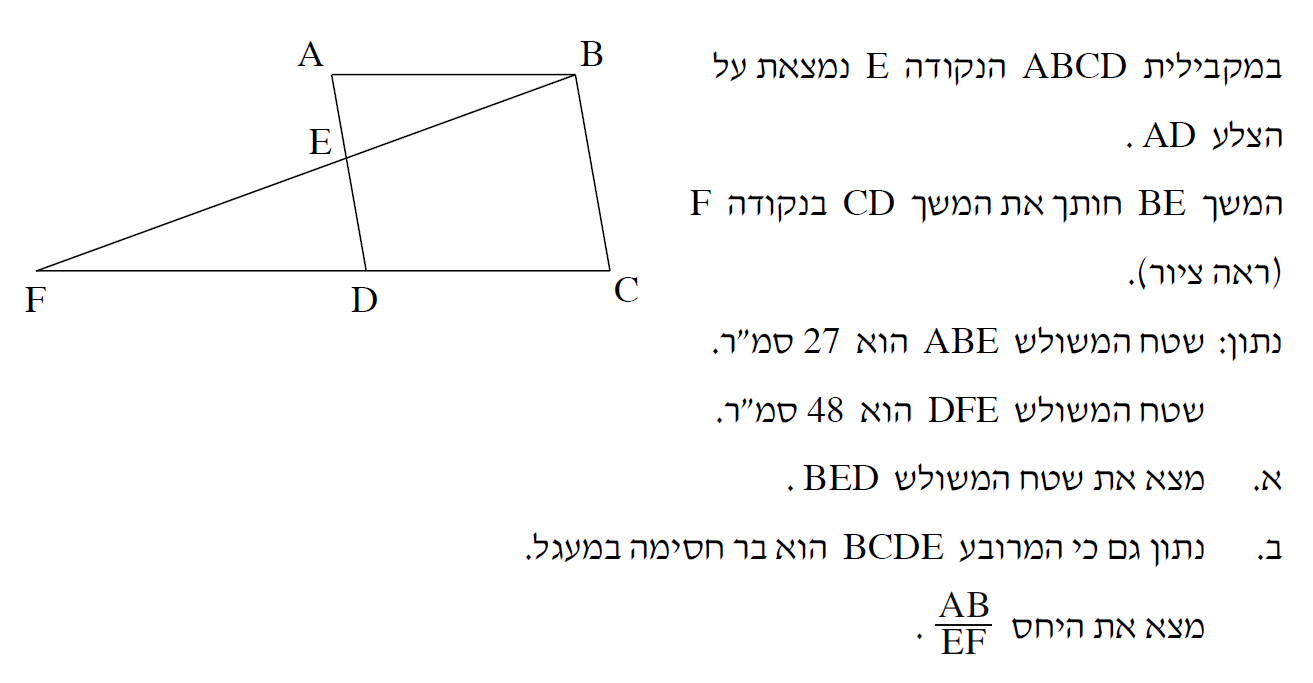
\includegraphics[width=\textwidth]{winter-2015-4}
\end{center}

\vspace{-5mm}

\textbf{סעיף א}

יש שתי דרכים לחשב את השטח של 
$\triangle BED$.
הראשונה היא לחשב את השטח של
$\triangle ABD$
ולהחסיר את השטח של
$\triangle ABE$.
לפי הסימונים בציור:
\[
S_{ABD}=\frac{1}{2}x(h_1+h_2)\,,\quad\quad S_{AEB}=\frac{1}{2}xh_1\,.
\]
אם נוכל לבטא את
$h_2$
במונחים של
$h_1$,
נוכל להחשב את
$S_{BED}=S_{ABD}-S_{AEB}$.

$\triangle ABE\sim \triangle DFE$
לפי ז.ז. בגלל הזוויות המתחלפות ב-%
$A,D$
ו-%
$B,F$.
לפי משפט
$100$%
ז "יחס השטחים שווה לריבוע יחס הדמיון":
\erh{12pt}
\begin{equationarray*}{rcl}
\frac{h_2}{h_1} &=& \sqrt{\frac{S_{DEF}}{S_{ABE}}} = \sqrt{\frac{48}{27}} = \frac{4}{3}\\
S_{BED} &=& S_{ABD}-S_{AEB}\\
&=& \frac{1}{2}x\left(h_1+\frac{4}{3}h_1\right)-\frac{1}{2}xh_1\\
%&=& \frac{1}{2}x\cdot \frac{4}{3}h_1\\
&=& \frac{4}{3}\left(\frac{1}{2}xh_1\right)=\frac{4}{3}\left(S_{ABE}\right)= \frac{4}{3}\cdot 27 = 36\,.
\end{equationarray*}

\vspace{-2mm}

\begin{center}
\selectlanguage{english}
\begin{tikzpicture}
\coordinate [label=below right:$D$] (D)  at (0,0);
\coordinate [label=below:$C$] (C)  at (4,0);
\coordinate [label=above right:$B$] (B)  at (3,3);
\coordinate [label=above left:$A$] (A)  at (-1,3);
\draw[thick,name path=para] (A) -- (B) -- (C) -- (D) -- cycle;
\node at (2,-.3) {$x$};
\node at (1.2,3.3) {$x$};
\path[name path=bf] (B) -- (-4,-.3);
\path[name path=df] (D) -- (-4,0);
\path[name intersections={of=bf and para,by={dummy,E}}];
\node[above left,xshift=-4pt] at (E) {$E$};
\path[name intersections={of=df and bf,by={F}}];
\node[below left] at (F) {$F$};
\draw[thick] (D) -- (F) -- (B);
\fill (A) circle (1.5pt);
\fill (B) circle (1.5pt);
\fill (C) circle (1.5pt);
\fill (D) circle (1.5pt);
\fill (E) circle (1.5pt);
\fill (F) circle (1.5pt);
\draw[thick,dashed] (E) |- (A);
\draw[thick,dashed] (E) |- (D);
\draw[thick,dashed] (B) -- (D);
\node at (-.1,2.4) {$h_1$};
\node at (-.8,.6) {$h_2$};
\end{tikzpicture}
\end{center}


הדרך השנייה לחשב את השטח של
$\triangle BED$
קשה לראות אבל החישוב מאוד פשוט. למשולשים 
$\triangle AEB,\triangle BED$
גובה זהה 
$h$
מהנקודה
$B$
ועד
$AD$.
יחס השטחים הוא הריבוע של יחס הצלעות
$AE,ED$
במשולשים 
$\triangle ABE,\triangle DFE$
שחישבנו לעיל:
\[
S_{BED} = \frac{4}{3}S_{AEB}=\frac{4}{3}\cdot 27 = 36\,.
\]
\vspace{-6mm}

\begin{center}
\selectlanguage{english}
\begin{tikzpicture}
\coordinate [label=below:$D$] (D)  at (0,0);
\coordinate (C)  at (4,0);
\coordinate [label=above right:$B$] (B)  at (3,3);
\coordinate [label=above left:$A$] (A)  at (-1,3);
\path[thick,name path=para] (A) -- (B) -- (C) -- (D) -- cycle;
\path[name path=bf] (B) -- (-4,-.3);
\path[name path=df] (D) -- (-4,0);
\path[name intersections={of=bf and para,by={dummy,E}}];
\node[left,xshift=-4pt] at (E) {$E$};
\draw[thick] (A) -- (B) -- (E) -- cycle;
\draw[thick] (E) -- (D) -- (B);
\fill (A) circle (1.5pt);
\fill (B) circle (1.5pt);
\fill (D) circle (1.5pt);
\fill (E) circle (1.5pt);
\coordinate (H) at ($(A)!(B)!(D)$);
\draw[thick,dashed] (B) -- node[above left] {$h$} (H);
\fill (H) circle (1.5pt);
\draw[rotate=20] (H) rectangle +(7pt,7pt);
\end{tikzpicture}
\end{center}

\vspace{-4mm}

\textbf{סעיף ב}

לכאורה, לא צריך את הנתון על המרובע כי
$\triangle ABE\sim \triangle DFE$.
אבל עיון מדוקדק יגלה שהיחס שחישבנו הוא 
$\displaystyle\frac{AB}{FD}$
ולא
$\displaystyle\frac{AB}{EF}$.

הנתון שהמרובע 
$BCDE$
בר חסימה במעגל מכוון למשפט
$56$
"ניתן לחסום מרובע במעגל אם ורק אם סכום זוג זוויות נגדיות שווה ל-%
$180^\circ$".
נסמן זוויות ונראה אם יוצא מזה משהו מועיל. נסמן ב-%
$\alpha$
את הזוויות הנגדיות של המקבילית
$A,C$
ואת הזוויות המתאימות בנקודות
$C,D$.
נסמן ב-%
$\beta$
את הזוויות המתחלפות ב-%
$B,F$.

סכום הזוויות במשולש הוא
$180$
ולכן הזוויות הקודקודיות ב-%
$E$
שוות ל-%
$180-(\alpha+\beta)$.
לפי זוויות משלימות
$\angle BED=\alpha+\beta$.
נפעיל את משפט
$56$
ונקבל:
\erh{2pt}
\begin{equationarray*}{rcl}
\angle BCD + \angle BED&=&180\\
\alpha+\alpha+\beta&=&180\\
\alpha&=&180-(\alpha+\beta)\\
\angle ABE&=&\angle EBA\\
\angle 	DFE&=&\angle EFD\,. 
\end{equationarray*}
המשולשים
$\triangle ABE, \triangle DFE$ 
שווה שוקיים! נשתמש ביחס שחישבנו בסעיף א:
\[
\frac{AB}{EF} = \frac{AB}{FD} = \frac{3}{4}\,.
\]


\begin{center}
\selectlanguage{english}
\begin{tikzpicture}[scale=1.1]
\coordinate [label=below right:$D$] (D)  at (0,0);
\coordinate [label=below:$C$] (C)  at (4,0);
\coordinate [label=above right:$B$] (B)  at (3,3);
\coordinate [label=above left:$A$] (A)  at (-1,3);
\draw[thick,name path=para] (A) -- (B) -- (C) -- (D) -- cycle;
\path[name path=bf] (B) -- (-4,-.3);
\path[name path=df] (D) -- (-4,0);
\path[name intersections={of=bf and para,by={dummy,E}}];
\node[above left,xshift=-4pt,yshift=2pt] at (E) {$E$};
\path[name intersections={of=df and bf,by={F}}];
\draw[thick] (D) -- (F) -- (B);
\fill (A) node[below right,xshift=2pt] {$\alpha$} circle (1.5pt);
\fill (B) node[below left,xshift=-22pt,yshift=1pt] {$\beta$} circle (1.5pt);
\fill (C) node[above left,xshift=-2pt] {$\alpha$} circle (1.5pt);
\fill (D) node[above left,xshift=-2pt] {$\alpha$} circle (1.5pt);
\fill (E) node[right,xshift=3pt,yshift=-5pt] {$\alpha+\beta$} circle (1.5pt);
\fill (F) node[below left] {$F$} node[above right,xshift=28pt,yshift=-2pt] {$\beta$} circle (1.5pt);
\node at ($(E)+(-55pt,0)$) {$180-(\alpha+\beta)$};
\draw[->] ($(E)+(-20pt,2pt)$) -- +(24pt,3pt);
\draw[->] ($(E)+(-20pt,-2pt)$) -- +(19pt,-3pt);
\end{tikzpicture}
\end{center}


%%%%%%%%%%%%%%%%%%%%%%%%%%%%%%%%%%%%%%%%%%%%%%%%%%%%%%%%%%%%%%%%%%%


\newpage
\end{comment}

\section{קיץ תשע"ד מועד ב}

\begin{center}
\selectlanguage{english}
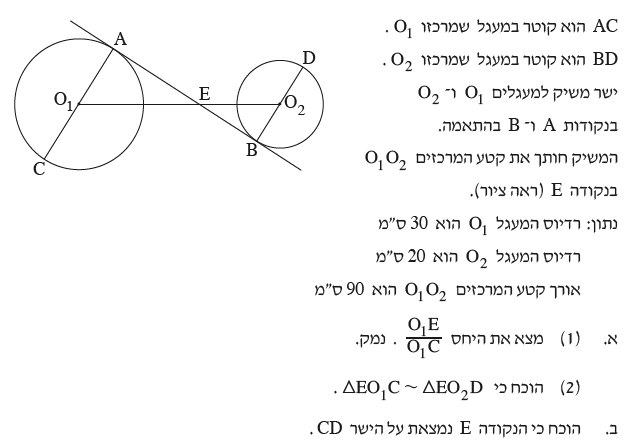
\includegraphics[width=.9\textwidth]{summer-2014b-4}
\end{center}

\vspace{-4ex}

\textbf{סעיף א}

$(1)$
כדי לסבך מעט את השאלה ביקשו את היחס בין
$O_1E$
ל-%
$O_1C$,
אבל 
$O_1A=O_1C$
כי הם רדיוסים. אם נוכיח ש-%
$\triangle O_1 A E\sim \triangle O_2 B E$,
נוכל להחשב את היחס המבוקש.

$AB$
משיק לשני המעגלים ולכן 
$\angle O_1 A E= \angle O_2 B E=90^\circ$
לפי משפט
$77$
"המשיק למעגל מאונך לרדיוס בנקודת ההשקה".
$\angle A E O_1=\angle B E O_2$
כי הן זוויות קודקודיות. מכאן ש-%
$\triangle O_1 A E\sim \triangle O_2 B E$
לפי ז.ז. נסמן ב-%
$x$
את אורכו של
$O_1 E$
ונקבל:
\erh{14pt}
\[
\begin{array}{l}
\displaystyle\frac{O_1 E}{O_2 E}= \frac{x}{90-x} = \frac{O_1A}{O_2B} = \frac{30}{20}\\
%2700-30x&=&20x\\
%x=54\\
\displaystyle\frac{O_1 E}{O_1 C} =\frac{O_1E}{O_1A} = \frac{54}{30}=\frac{9}{5}\,.
\end{array}
\]
\vspace{-2ex}

\begin{center}
\selectlanguage{english}
\begin{tikzpicture}[scale=1.2]
\coordinate (o1) at (0,0);
\coordinate (A)  at (50:2);
\draw[rotate=-130] (A) rectangle +(4pt,4pt);
\coordinate (C) at (-130:2);
\node [draw,circle through=(C)] at (o1) {};
\draw (A) -- (C);
\coordinate (o2) at (5,0);
\coordinate (D)  at ($(o2) + (50:1)$);
\coordinate (B)  at ($(o2) + (-130:1)$);
\draw[rotate=50] (B) rectangle +(4pt,4pt);
\node [draw,circle through=(B)] at (o2) {};
\draw (B) -- (D);
\draw[name path=diameters] (o1) -- node[below,xshift=4mm] {$90$} (o2);
\draw[name path=tangents] ($ (A) ! -.5 ! (B) $) -- ($ (A) ! 1.5 ! (B) $);
\path [name intersections={of=diameters and tangents,by={E}}];
\fill (A) node[above,xshift=2pt] {$A$} circle(1pt);
\fill (B) node[below,xshift=-4pt] {$B$} circle(1pt);
\fill (C) node[below,xshift=-2pt] {$C$} circle(1pt);
\fill (D) node[above,xshift=4pt] {$D$} circle(1pt);
\fill (E) node[above,xshift=2pt] {$E$} circle(1pt);
\fill (o1) node[left,xshift=-2pt] {$O_1$} circle(1pt);
\fill (o2) node[right,xshift=2pt] {$O_2$} circle(1pt);
\path (A)  -- node[left,xshift=-2pt] {$30$} (o1);
\path (o1) -- node[left,xshift=-2pt] {$30$} (C);
\path (D)  -- node[right,xshift=1pt] {$20$} (o2);
\path (o2) -- node[right,xshift=1pt] {$20$} (B);
\path (o1) -- node[above] {$x$} (E);
\end{tikzpicture}
\end{center}


$(2)$
נראה שאפשר להשתמש באותה שיטה כדי להוכיח שהמשולשים 
$\triangle E O_1 C \sim \triangle E O_2 D$
דומים. אבל, כפי שמרמז סעיף ב, איננו יודעים שהנקודה
$E$
נמצאת על הקו הישר
$CD$,
ולכן איננו יכולים להניח ש-%
$\angle O_1 E C, \angle O_2 E D$
הן זוויות הקודקודיות )שוות(. במקום זה, נשתמש בעובדה שהקוטרים מקביליים ולהוכיח בצורה ישירה שהמשולשים דומים.

$AC\|DB$
כי שניהם ניצבים לקו
$O_1O_2$,
ולכן 
$\angle C O_1 E=\angle D O_2 E=\alpha$
כי הן זוויות מתחלפות. כל הרדיוסים של מעגל שווים, כך ש-%
$O_1C=O_1A, O_2B=O_2D$.
הוכחנו ש-%
$\triangle E O_1 A \sim \triangle E O_2 B$,
ולכן
\[
\frac{O_1E}{O_2E}=\frac{O_1C}{O_2D}\,,
\]
ו-%
$\triangle E O_1 C \sim \triangle E O_2 D$.

\vspace{-4mm}

\begin{center}
\selectlanguage{english}
\begin{tikzpicture}[scale=1.2]
\coordinate (o1) at (0,0);
\coordinate (A)  at (50:2);
\draw[rotate=-130] (A) rectangle +(4pt,4pt);
\coordinate (C) at (-130:2);
\node [draw,circle through=(C)] at (o1) {};
\draw (A) -- (o1);
\draw[dashed,very thick] (o1) -- (C);
\coordinate (o2) at (5,0);
\coordinate (D)  at ($(o2) + (50:1)$);
\coordinate (B)  at ($(o2) + (-130:1)$);
\node[below right] at (o1) {$\alpha$};
\node[above left,xshift=1mm] at (o2) {$\alpha$};
\draw[rotate=50] (B) rectangle +(4pt,4pt);
\node [draw,circle through=(B)] at (o2) {};
\draw (B) -- (o2);
\draw[dashed,very thick] (o2) -- (D);
\draw[name path=diameters,dashed,very thick] (o1) -- node[below,xshift=6mm,yshift=-2mm] {$90$} (o2);
\draw[name path=tangents] ($ (A) ! -.5 ! (B) $) -- ($ (A) ! 1.5 ! (B) $);
\path [name intersections={of=diameters and tangents,by={E}}];
%\path (A)  -- node[left,xshift=-1mm] {\textsf{\small 30}} (o1);
%\path[dashed,very thick] (o1) -- node[left,xshift=-1mm] {\textsf{\small 30}} (C);
%\path (D)  -- node[right,xshift=1mm] {\textsf{\small 20}} (o2);
%\path (o2) -- node[right,xshift=1mm] {\textsf{\small 20}} (B);
\path[dashed,very thick] (o1) -- node[above] {$x$} (E);
\draw[dashed,very thick] (C) -- (D);
\fill (A) node[above,xshift=2pt] {$A$} circle(1pt);
\fill (B) node[below,xshift=-4pt] {$B$} circle(1pt);
\fill (C) node[below,xshift=-2pt] {$C$} circle(1pt);
\fill (D) node[above,xshift=4pt] {$D$} circle(1pt);
\fill (E) node[above,xshift=2pt] {$E$} circle(1pt);
\fill (o1) node[left,xshift=-2pt] {$O_1$} circle(1pt);
\fill (o2) node[right,xshift=2pt] {$O_2$} circle(1pt);
\path (A)  -- node[left,xshift=-2pt] {$30$} (o1);
\path (o1) -- node[left,xshift=-2pt] {$30$} (C);
\path (D)  -- node[right,xshift=1pt] {$20$} (o2);
\path (o2) -- node[right,xshift=1pt] {$20$} (B);
\path (o1) -- node[above] {$x$} (E);
\end{tikzpicture}
\end{center}

\vspace{-4mm}

\textbf{סעיף ב}

נתבונן בזוויות סביב הנקודה
$E$
שנמצאת על 
$CD$
אם הזווית 
$\angle AED$
משלימה לזווית
$\angle AEC$.
הוכחנו
$\triangle O_1 E C\sim \triangle O_2 E D$
ו-%
$\triangle O_1 A E \sim \triangle O_2 B E$,
ונסמן את הזוויות השוות
$\alpha,\beta$.
נתון ש-%
$AB$
הוא קו ישר ו-% 
$\angle AED$
משלימה ל-%
$\angle DEB$,
כך ש-%
$\angle AED = 180^\circ - (\alpha + \beta)$.
נבדוק עם 
$\angle AED$
משלימה ל-%
$\angle AEC$:
\[
\angle AED + \angle AEC = (180^\circ - (\alpha + \beta)) + (\alpha + \beta) = 180^\circ\,.
\]



\begin{center}
\selectlanguage{english}
\begin{tikzpicture}[scale=1.1]
\coordinate [label=left:$O_1$] (o1) at (0,0);
\coordinate [label=above:$A$] (A)  at (50:2);
\coordinate [label=below:$C$] (C) at (-130:2);
\node [circle through=(C)] at (o1) {};
\draw (A) -- (C);
\coordinate [label=right:$O_2$] (o2) at (5,0);
\coordinate [label=above:$D$] (D)  at ($(o2) + (50:1)$);
\coordinate [label=below:$B$] (B)  at ($(o2) + (-130:1)$);
\node [circle through=(B)] at (o2) {};
\draw (B) -- (D);
\draw[name path=diameters] (o1) -- (o2);
\draw[name path=tangents] ($ (A) ! -.1 ! (B) $) -- ($ (A) ! 1.1 ! (B) $);
\path [name intersections={of=diameters and tangents,by={[label=above:$E$]E}}];
\path (A)  -- (o1);
\path (o1) -- (C);
\path (D)  -- (o2);
\path (o2) -- (B);
\path (o1) -- (E);
\node[xshift=-20pt,yshift=7pt] at (E) {$\alpha$};
\node[xshift=20pt,yshift=-7pt] at (E) {$\alpha$};
\node[xshift=38pt,yshift=6pt] at (E) {$\beta$};
\node[xshift=-38pt,yshift=-7pt] at (E) {$\beta$};
\draw (C) -- (D);
\end{tikzpicture}
\end{center}
%%%%%%%%%%%%%%%%%%%%%%%%%%%%%%%%%%%%%%%%%%%%%%%%%%%%%%%%%%%%%%%%%%%

\begin{comment}

\newpage
\section{קיץ תשע"ד מועד א}

\begin{center}
\selectlanguage{english}
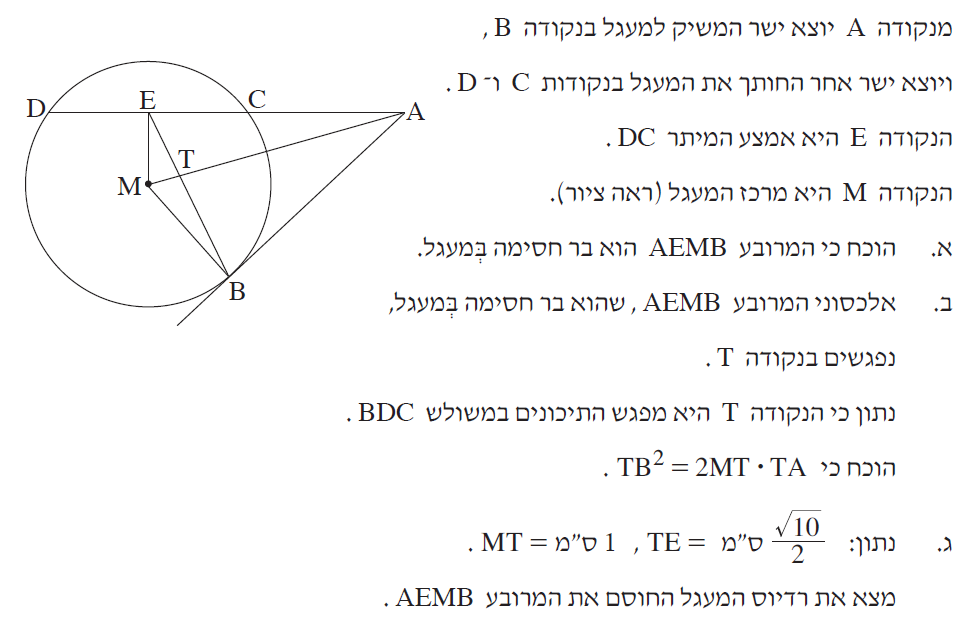
\includegraphics[width=\textwidth]{summer-2014a-4}
\end{center}


\textbf{סעיף א}
המשפטים שיכולים להיות שימושיים הם:
$(103)$
כאשר יש משיק וקו שחותך את המעגל, 
$AB^2=AC\cdot AD$.
$(77)$
הרדיוס והמשיק מאונכים זה לזה
$MB \perp PA$. 
$(68)$
קטע ממרכז המעגל החוצה מיתר מאונך למיתר.
$(56)$
ניתן לחסום מרובע במעגל רק אם סכום הזוויות הנגדיות שווה ל-%
$180^\circ$.

\begin{center}
\selectlanguage{english}
\begin{tikzpicture}[scale=1]
\coordinate [label=left:$M$] (M) at (0,0);
\coordinate [label=below right:$B$] (B)  at (-45:3);
\coordinate [label=right:$A$] (A) at (6,2);
\node [draw,thick,circle through=(B),name path=circ] at (M) {};
\draw[name path=tangents,thick] (A) -- ($ (A) ! 1.5 ! (B) $);
\path[name path=adc] (A) -- +(-9,0);
\path[name intersections={of=adc and circ,by={[label=above right:$C$]C,[label=above left:$D$]D}}];
\draw[thick] (A) -- (D);
\draw[thick,name path=am] (A) -- (M);
\draw[thick] (B) -- (M);
\path[name path=mid] (M) -- +(0,3.5);
\path[name intersections={of=mid and adc,by={[label=above:$E$]E}}];
\draw[thick,name path=eb] (E) -- (B);
\draw[thick] (E) -- (M);
\path[name intersections={of=eb and am,by={T}}];
\node[above,xshift=4pt] at (T) {$T$};
\fill (M) circle (1.5pt);
\fill (A) circle (1.5pt);
\fill (B) circle (1.5pt);
\fill (C) circle (1.5pt);
\fill (D) circle (1.5pt);
\fill (E) circle (1.5pt);
\end{tikzpicture}
\end{center}

משני המפשטים אנו יודעים ש-%
$\angle MEA + \angle MBA = 90^\circ + 90^\circ = 180^\circ$.
לפי משפט
$(106)$,
סכום הזוויות הפנימיות של מרובע הוא 
$360^\circ$,
ולכן:
\[
\angle EMB + \angle EAB = 360^\circ -(\angle MEA + \angle MBA) = 360^\circ - 180^\circ=180^\circ\,.
\]

\textbf{סעיף ב}

נכין איור עם המידע הרלוונטי בלבד. המעגל החוסם את המרובע
$AEMB$
והמשולש
$BDC$:
\vspace{-22mm}
\begin{center}
\selectlanguage{english}
\begin{tikzpicture}[scale=1]
\coordinate [label=left:$M$] (M) at (0,0);
\coordinate [label=below right:$B$] (B)  at (-45:3);
\coordinate [label=right:$A$] (A) at (6,2);
\node [circle through=(B),name path=circ] at (M) {};
\draw[name path=tangents,thick] (A) -- (B); %($ (A) ! 1.1 ! (B) $);
\path[name path=adc] (A) -- +(-9,0);
\path[name intersections={of=adc and circ,by={[label=above right:$C$]C,[label=above left:$D$]D}}];
\draw[thick,name path=am] (A) -- (M);
\draw[thick] (B) -- (M);
\path[name path=mid] (M) -- +(0,3.5);
\path[name intersections={of=mid and adc,by={[label=above left:$E$]E}}];
\draw[thick,name path=eb] (E) -- (B);
\draw[thick] (E) -- (M);
\path[name intersections={of=eb and am,by={T}}];
\node[above,xshift=4pt] at (T) {$T$};
\fill (M) circle (1.5pt);
\fill (A) circle (1.5pt);
\fill (B) circle (1.5pt);
\fill (C) circle (1.5pt);
\fill (D) circle (1.5pt);
\fill (E) circle (1.5pt);
\draw[thick,dashed] (C) -- (B) -- (D) -- cycle;
\tkzCircumCenter(M,E,A)\tkzGetPoint{O}
\tkzDrawCircle[thick](O,A)
\end{tikzpicture}
\end{center}
\vspace{-18mm}
אפשר לראות שקטעי הקווים
$MA,BE$
הם מיתרים נחתכים של המעגל החוסם. לפי משפט
$(101)$
$TB\cdot TE=MT\cdot TA$.
נתון שהנקודה
$T$
היא מפגש התיכונים, ולכן לפי משפט
$(46)$,
$TB/TE=2$.
כעת החישוב פשוט:
\begin{equationarray*}{rcl}
TB\cdot TE &=& MT\cdot AT\\
TB\cdot (TB/2) &=& MT\cdot AT\\
TB^2 &=& 2MT\cdot AT\,.
\end{equationarray*}

\textbf{סעיף ג}
$\angle MBA$
היא זווית ישרה, ולכן לפי משפט
$(74)$
$MA$
הוא קוטר. עם הערכים הנתונים
$MT=1, TE=\frac{\sqrt{10}}{2}$
נחשב את הרדיוס:
\begin{equationarray*}{rcl}
R &=& \frac{1}{2}MA\\
&=&\frac{1}{2}(MT+TA)\\
%&=&\frac{1}{2}(1+TA)\\
&=&\frac{1}{2}(1+\frac{TB^2}{2\cdot 1})\\
&=&\frac{1}{2}(1+2TE^2)\\
&=&\frac{1}{2}(1+2\frac{10}{4})\\
&=&3\,.
\end{equationarray*}

%%%%%%%%%%%%%%%%%%%%%%%%%%%%%%%%%%%%%%%%%%%%%%%%%%%%%%%%%%%%%%%%%%%


\section{חורף תשע"ד}

\begin{center}
\selectlanguage{english}
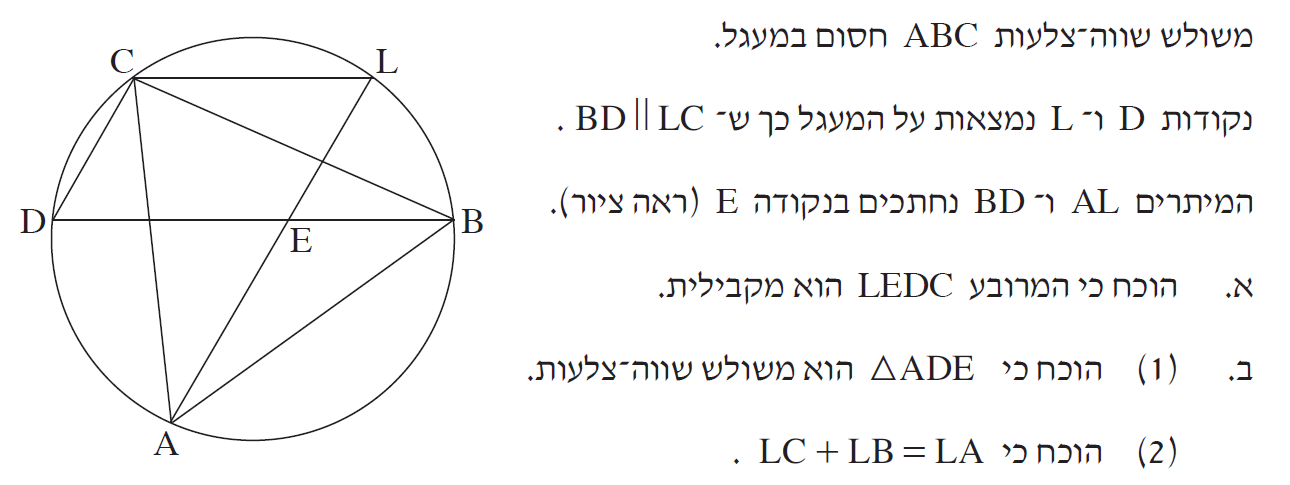
\includegraphics[width=\textwidth]{winter-2014-4}
\end{center}

\textbf{\R{סעיף א}}
אין לנו מידע על מיתרים המגדירים את המרובע שאמור להיות מקבילית, ולכן ננסה להוכיח אל ידי אפיון המקבילית כמרובע עם זוויות נגדיות שוות )משפט 92( או עם צלעות נגדיות מקביליות )משפט 03(. נתון שזוג אחד של צלעות
$CL,DE$
מקבילי, אז ננסה להוכיח שהזוג
$DC,EL$
מקבילי.

כאשר יש "מספר רב" של מיתרים, סביר שיש זוויות הנשענות על אותו מיתר או קשת ולכן הן שוות )משפטים 07,27(.

נסמן את הזוויות של המשלוש 
$\alpha=60^\circ$.
\begin{center}
\selectlanguage{english}
\begin{tikzpicture}%[scale=.75]
\coordinate (left) at (0,0);
\coordinate (right) at (6,0);
\coordinate (apath) at (0,-4);
\coordinate (bpath) at (7,1);
\coordinate (cpath) at (1.5,4);
\path [name path=chord1] (apath) -- (bpath);
\path [name path=chord2] (apath) -- (cpath);
\coordinate (center) at ($ (right)!.5!(left) $);
\node [draw,thick,circle through=(left),name path=circ] at (center) {};
\path [name intersections={of=circ and chord1,by={b,a}}];
\path [name intersections={of=circ and chord2,by={c,dummy1}}];
\fill (a) circle (2pt) node[below left] {$A$} node[xshift=4pt,yshift=15pt] {$\alpha$};
\fill (b) circle (2pt) node[right] {$B$} node[xshift=-15pt,yshift=-5pt] {$\alpha$};
\fill (c) circle (2pt) node[above left] {$C$} node[xshift=6pt,yshift=-10pt] {$\alpha$};
\path [name path=chord3] (b) -- +(-7,0);
\path [name intersections={of=circ and chord3,by={d}}];
\fill (d) circle (2pt) node[left] {$D$};
\path [name path=chord4] (c) -- +(4,0);
\path [name intersections={of=circ and chord4,by={l}}];
\fill (l) circle (2pt) node[above right] {$L$};
%% Draw triangle
\draw[thick] (a) -- (b) -- (c) -- cycle;
\draw[thick] (b) -- (d) -- (c) -- (l);
\draw[thick,name path=chord5] (l) -- (a);
\draw [name intersections={of=chord5 and chord3,by={e}}];
\fill (e) circle (2pt) node[below right] {$E$};
%% Angles
\draw[thick] +($ (a)!.15!(b) $) arc [radius=18pt,start angle=20,delta angle=82];
\draw[thick] ($ (c)!.15!(b) $) arc [radius=18pt,start angle=-20,delta angle=-75];
\draw[thick] ($ (b)!.15!(c) $) arc [radius=18pt,start angle=140,delta angle=82];
\end{tikzpicture}
\end{center}
$\angle CLA=\angle CBA$
כי הן נשענות על המיתר
$AC$.
$\angle CDB=\angle CAB$
כי הן נשענות על המיתר
$BC$.
נתון ש-%
$CL\|DB$
והזוויות המתחלפות שוות
$\angle LEB = \angle CLA$.
מכאן:
\begin{equationarray*}{rcl}
60^\circ=\angle CBA &=& \angle CLA =\angle LEB\\
60^\circ=\angle CAB &=& \angle CDB\,.
\end{equationarray*}
$DC\|LE$
כי
$\angle LEB,\angle CDB$
הן זוויות מתאימות שוות.

\textbf{\R{סעיף ב}}
$(1)$
שוב, אין לנו מידע על אורכי הקווים לכן ננסה להוכיח שכל הזוויות של המשולש
$\triangle ADE$
שוות ל-%
$60^\circ$.
כמובן, שמספיק להוכיח ששתי זוויות שוות ל-%
$60^\circ$
כי השלישית צריכה להשלים ל-%
$180^\circ$,
סכום הזוויות במשולש.

בסעיף א הוכחנו ש-%
$\angle LEB=60^\circ$
ו-%
$\angle DEA=60^\circ$
כי הן זוויות קודקודיות. ננסה להוכיח ש-%
$\angle DAE=60^\circ$
או
$\angle ADE=60^\circ$
על ידי חיפוש זוויות אחרת הנשענת על אותו מיתר. בדיקה קצרה מראה ש-%
$\angle ACB=60^\circ, \angle ADE=\angle ADB$
נשענות על המיתר
$AB$.

$(2)$
נקח רמז מהחלק הראשון של הסעיף. אם
$\triangle ADE$
שווה צלעות, אז
$AE=DE$
ו-%
$DE=CL$
כי הן צלעות נגדיות של מקבילית. לכן:
\[
LA-LC=(LE+AE)-LC=(LE+LC)-LC=LE\,.
\]
נשאר להוכיח
$LE=LB$.
הוכחנו ש-%
$\angle LEB=60^\circ$,
כך שאם נוכיח שזווית נוספת ב-%
$\triangle LEB$
שווה ל-%
$60^\circ$
נקבל משלוש שווה צלעות ו-%
$LE=LB$.
שוב נחפש זוויות הנשענות על אותו מיתר ונקבל ש-%
$\angle BLA=\angle BCA$
כי שתיהן נשענות על המיתר
$AB$.

תוך כי נסיונות לפתור מצאתי הוכחה אחרת מעניינת. 
$\angle LBE=\angle LBD, \angle DCL$
נשענות או אותו קשה אבל
\textbf{מצדדים נגדיים}.
הזווית שנשענת על קשת שווה למחצית הקשת, ולכן אם סכום שתי הקשתות הוא כל המעגל, סכום הזוויות שווה 
$180^\circ$.
אנו יודעים ש-%
$\angle DCL=120^\circ$
כך ש-%
$\angle LBE=\angle LBD=60^\circ$.

%%%%%%%%%%%%%%%%%%%%%%%%%%%%%%%%%%%%%%%%%%%%%%%%%%%%%%%%%%%%%%%%%%%

\newpage

\section{המלצות}

\begin{itemize}
\item
חשוב לצייר ציורים 
\textbf{וגדולים}.
בתהליך הפתרון אנו מסמנים את המידע המצטבר על הזוויות והצלעות ויש לדאוג שיהיה מספיק מקום.

\item
על הציורים להיות ברורים תוך שימוש בסרגל ומחוגה. אבל 
\textbf{אין לסמוך על הציור}.
לעתים, מה שנראה ברור בציור הוא בדיוק מה שעלינו להוכיח. בעמוד 
\L{\pageref{}}
הבאתי הוכחה שכל משולש הוא שווה שוקיים, כאשר ההוכחה מסתמכת על ציור שאינו נכון.

\item
אני מעדיף לסמן זוויות עם אות (יוונית)
$\alpha$
ולא על ידי ציון שלושת הנקודות המגדירות אותה
$\angle ABC$,
כי קשה לעקוב אחר הנקודות השונות.

\item
לשאלות מספר סעיפים. במקרים רבים כדאי לצייר ציורים נפרדים לכל סעיף תוך העלמת מידע לא רלוונטי. בבחינה של בבבבב קל לראות את דרך הפתרון רק כאשר מסלקים קווים לא רלוונטיים.

\item
רצוי לרשום את המשפטים שיכולים להיות רלוונטיים לפני שמנסים לפתור את השאלה. זה יכול לכוון לפתרון. עם זאת יש לזכור שלא כל המשפטים נחוצים. בבחינה של בבבב היחס בין משיק לקו החותך מעגל נראה רלוונטי אבל אין בו צורך.

\item
יש משפטים שזוכרים בקלות כי הם די אינטואטיביים, למשל, שמשולשים חופפים לפי צ.צ.צ. ודומים לפי ז.ז. יש משפטים אחרים שקשה יותר לזכור אותם ושהוכחת נכונותם לא קלה.
\url{}
עם ציוריים צבעוניים של מבחר משפטים כדי לעזור לזכור אותם. מה שקשה לזכור מניסוח מילולי מסורבל. נספח ב מכיל ציורים עבור חלק מהמשפטים המתקדמים יותר.

\item
כאשר שואלים על שטחים של משולשים, כדאי לחפש גבהים משותפים. אנו רגילים לראות גבהים מנקודה לקו אופקי, אבל קיימים גבהים מכל נקודה לקו ממול ללא קשר למצג שלו על הנייר.

\item
כדי להוכיח חפיפה של משלושים ישר זווית מספיק להוכיח שוויון של צלע אחד ושיוון של זווית חדה אחת. אם הצלע הוא בין זווית חדה לבין הזווית הישרה, החפיפה היא לפי ז.צ.ז. אם הצלע הוא בין שתי הזוויות החדות, הזווית שערכה 
$\alpha$
והזווית השניה 
$\beta$,
אזי
$\beta=90^\circ-\alpha$,
ושוב יש ז.צ.ז. אני מניח שבבחינה צריך להזכיר עובדה זו, אבל כאשר מחפשים דרך להוכיח חפיפה, קיצור דרך זו יכול להועיל.
%
%קל לזכור מציור:
%\begin{quote}
%$45.$
%שלושת התיכונים במשולש נחתכים בנקודה אחת.\\
%$46.$
%נקודת חיתוך התיכונים מחלקת כל תיכון ביחס 2:1.\\
%)החלק הקרוב לקדקוד הוא פי 2 מהחלק האחר(.
%\end{quote}
%\begin{center}
%\selectlanguage{english}
%\begin{tikzpicture}[scale=1.1]
%\coordinate (a) at (0,0);   % Points of the triangle
%\coordinate (b) at (6,0);
%\coordinate (c) at (4,3);
%% Coordinates of bisectors
%\coordinate (ab) at ($(a)!.5!(b)$);
%\coordinate (bc) at ($(b)!.5!(c)$);
%\coordinate (ac) at ($(a)!.5!(c)$);
%% Draw the triangle and bisectors
%\draw[blue,very thick] (a) -- node[above] {$\bm{x}$} (ac) -- node[above] {$\bm{x}$} (c);
%\draw[red,very thick] (b) -- node[right] {$\bm{y}$} (bc) -- node[right] {$\bm{y}$} (c);
%\draw[green!60!black,very thick] (a) -- node[below] {$\bm{z}$} (ab) -- node[below] {$\bm{z}$} (b);
%\draw[very thick,red,name path=da] (a) -- (bc);
%\draw[very thick,blue,name path=db] (b) -- (ac);
%\draw[very thick,green!60!black,name path=dc] (c) -- (ab);
%% Get their intersection
%\path [name intersections={of=da and db,by={intersection}}];
%% Labels
%\path (a) -- node[above,red] {$\bm{2a}$} (intersection);
%\path (bc) -- node[above,red] {$\bm{a}$} (intersection);
%\path (b) -- node[above,blue] {$\bm{2b}$} (intersection);
%\path (ac) -- node[above,blue] {$\bm{b}$} (intersection);
%\path (c) -- node[right,green!60!black] {$\bm{2c}$} (intersection);
%\path (ab) -- node[right,green!60!black] {$\bm{c}$} (intersection);
%% Points at the intersections
%\fill (intersection) circle (2pt);
%\fill (ab) circle (2pt);
%\fill (ac) circle (2pt);
%\fill (bc) circle (2pt);
%\end{tikzpicture}
%\end{center}

\end{itemize}

%%%%%%%%%%%%%%%%%%%%%%%%%%%%%%%%%%%%%%%%%%%%%%%%%%%%%%%%%%%%%%%%%%%
%%%%%%%%%%%%%%%%%%%%%%%%%%%%%%%%%%%%%%%%%%%%%%%%%%%%%%%%%%%%%%%%%%%


\newpage

\begin{center}
\textbf{\large נספח א: אין לסמוך על איורים!}
\end{center}
הנה הוכחה "נכונה"
\textbf{\R{שכל}}
משולש שווה שוקיים!

נתון משולש שרירותי 
$ABC$,
תהי
$P$
נקודת החיתוך בין חוצה הזווית של
$\angle BAC$
לבין האנך האמצעי של 
$BC$.
סמן ב-%
$D,E,F$
את נקודות החיתוך של האנחים מ-%
$P$
לצלעות
$BC,AB,AC$.

$\triangle APE\cong \triangle APF$
כי הם משולשים ישר זווית עם זוויות שוות
$\alpha$
וצלע $AP$ משותף.

$\triangle DPB\cong \triangle DPC$
לפי צ.ז.צ. כי 
$PD$
הוא צלע משותף, ו-%
$BD=DC=a$
כי 
$PD$
הוא האנך האמצעי ל-%
$BC$.

$\triangle EPB\cong \triangle FPC$,
כי
$EP=PF$
לפי החפיפה הראשונה, ו-%
$PB=PC$
לפי החפיפה השנייה.

נחבר את השוויונות ונקבל:
\[
AB=AE+EB=AF+FC=AC\,.
\]
$\triangle ABC$
שווה שוקיים!
\begin{center}
\selectlanguage{english}
\begin{tikzpicture}[scale=1.3]
\coordinate (P) at (0,0);
\node[xshift=4mm,yshift=1mm] at (P) {$P$};
\coordinate [label=left:$B$] (B)  at (-2,-2);
\coordinate [label=right:$C$] (C)  at (4,-2);
\coordinate [label=above:$A$] (A)  at (-1,2);
\node[below,yshift=-12pt,xshift=2pt] at (A) {$\alpha$};
\node[below,yshift=-12pt,xshift=15pt] at (A) {$\alpha$};
\draw (A) -- (B);
\draw (A) -- (C);
\draw (B) -- (C);
\draw (A) -- (P);
\draw (B) -- (P);
\draw (C) -- (P);
\coordinate[label=left:$E$] (E) at ($ (A) ! .44 ! (B) $);
\draw[rotate=-100] (E) rectangle +(4pt,4pt);
\draw (P) -- (E);
\coordinate[label=right:$F$] (F) at ($ (A) ! .33 ! (C) $);
\draw[rotate=-132] (F) rectangle +(4pt,4pt);
\draw (P) -- (F);
\coordinate[label=below:$D$] (D) at ($ (B) ! .33 ! (C) $);
\draw (D) rectangle +(4pt,4pt);
\draw (P) -- (D);
\node[left] at ($ (A) ! .5 ! (E) $) {};
\node[left] at ($ (B) ! .5 ! (E) $) {};
\node[below] at ($ (B) ! .5 ! (D) $) {$a$};
\node[below] at ($ (C) ! .5 ! (D) $) {$a$};
\node[right,xshift=2pt] at ($ (A) ! .5 ! (F) $) {};
\node[right,xshift=2pt] at ($ (C) ! .5 ! (F) $) {};
\fill (A) circle(1pt);
\fill (B) circle(1pt);
\fill (C) circle(1pt);
\fill (D) circle(1pt);
\fill (E) circle(1pt);
\fill (F) circle(1pt);
\fill (P) circle(1pt);
\end{tikzpicture}
\end{center}
הבעיה בהוכחה היא שהאיור אינו נכון כי הנקודה
$P$
נמצאות
\textbf{\R{מחוץ}}
למשולש:
\begin{center}
\selectlanguage{english}
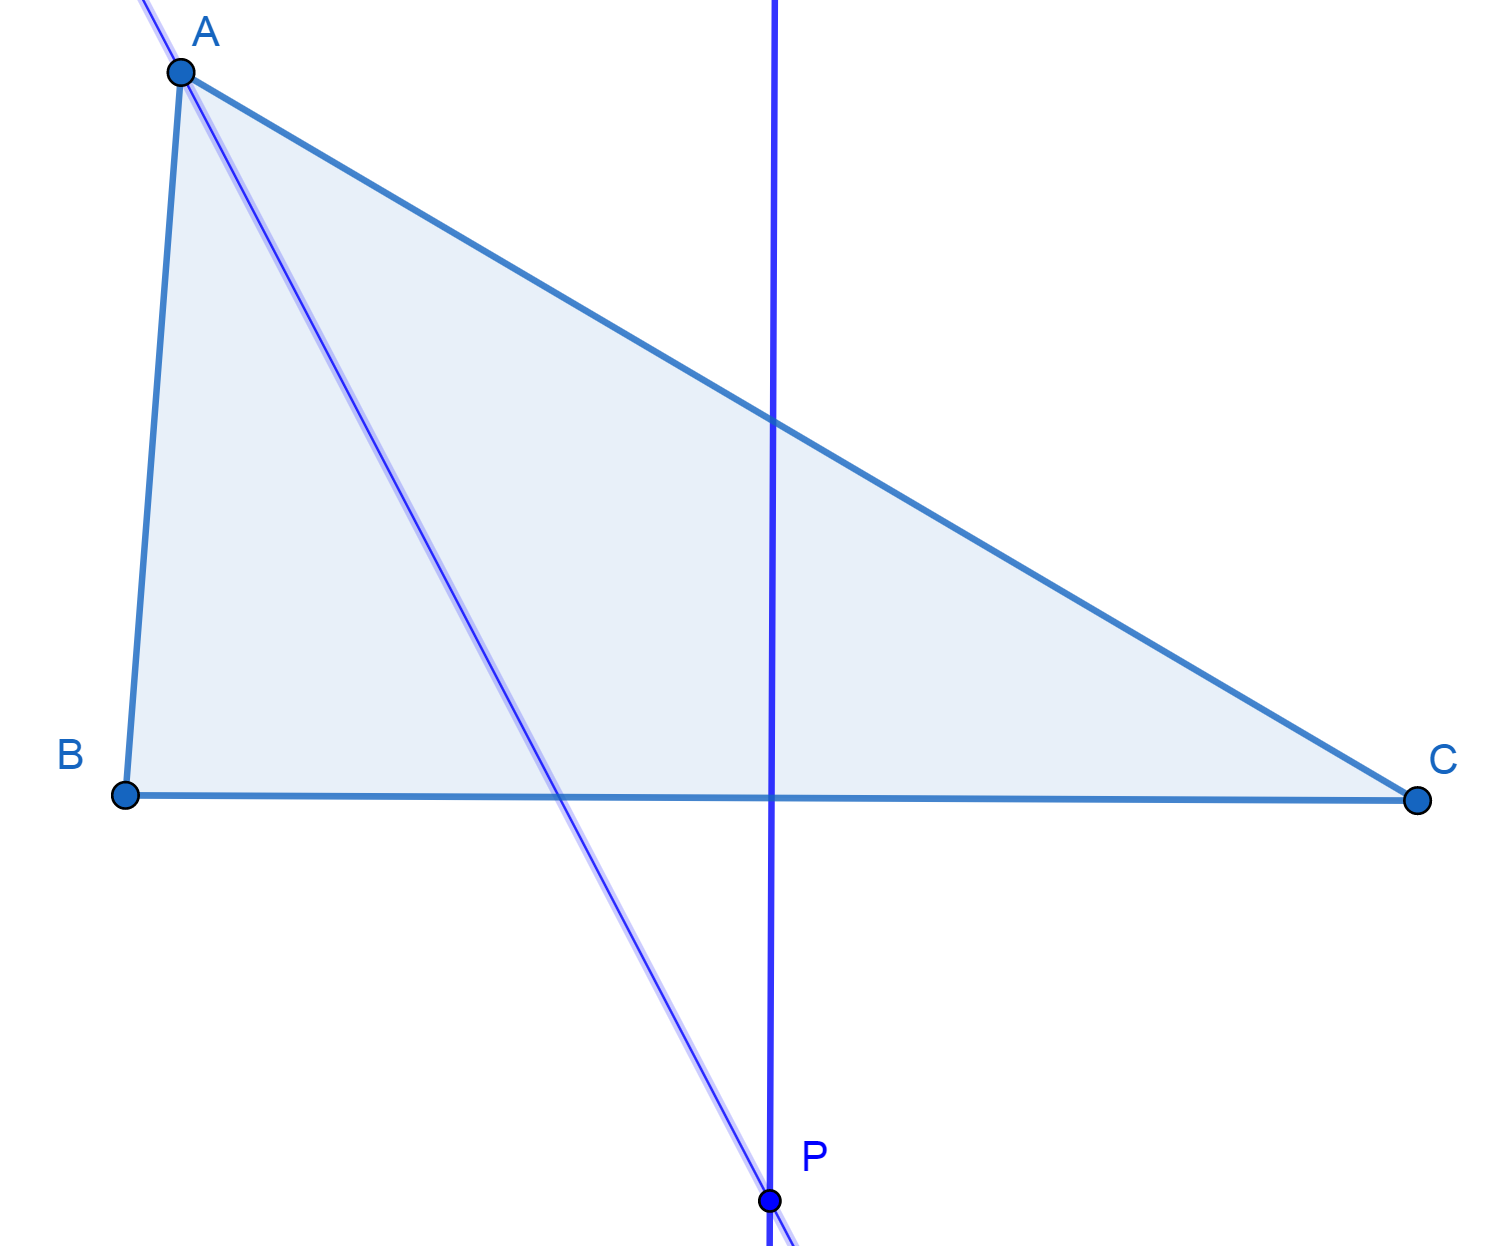
\includegraphics[width=.5\textwidth]{isoceles}
\end{center}

%%%%%%%%%%%%%%%%%%%%%%%%%%%%%%%%%%%%%%%%%%%%%%%%%%%%%%%%%%%%%%%%%%%
%%%%%%%%%%%%%%%%%%%%%%%%%%%%%%%%%%%%%%%%%%%%%%%%%%%%%%%%%%%%%%%%%%%
\newpage


\begin{center}
\textbf{\large נספח ב: ייצוג גרפי של משפטים בגיאומטריה}
\end{center}

%\bigskip\bigskip

%
% Thale's theorems
%
\selectlanguage{english}
\hspace*{-8mm}
\begin{minipage}[t]{.45\textwidth}
%\begin{center}
%\selectlanguage{hebrew}
%\textsf{משפטי תאלס}
%\end{center}
\begin{tikzpicture}[scale=1.2]
% Points of the triangle
\coordinate (a) at (0,0);
\coordinate (b) at (6,0);
\coordinate (c) at (4,3);
% Midpoints of the sides
\coordinate (mid1) at ($(a)!.5!(c)$);
\coordinate (mid2) at ($(b)!.5!(c)$);
% Draw the base and median
\draw[very thick,orange!80!black] (a) -- node[below] {$\bm{f}$} (b);
\draw[very thick,pink!60!black] (mid1) -- node[above] {$\bm{e}$} (mid2);
% Get the median
\coordinate (midbase) at ($(a)!.5!(b)$);
% Draw the triangle, sides in two parts
\draw[very thick,red] (a) -- node[above] {$\bm{b}$} (mid1);
\draw[very thick,blue] (mid1) -- node[above] {$\bm{a}$} (c);
\draw[very thick,green!60!black] (b) -- node[above,xshift=2pt] {$\bm{d}$} (mid2);
\draw[very thick,magenta] (mid2) -- node[above,xshift=2pt] {$\bm{c}$} (c);
% Dots at the midpoints
\fill (mid1) circle (2pt);
\fill (mid2) circle (2pt);
% Display first formula in color
\begin{scope}[xshift=2.5cm,yshift=.9cm]
\node[anchor=base,blue] at (0,0) {$\bm{a}$};
\node[anchor=base] at (.2,0) {$\bm{/}$};
\node[anchor=base,red] at (.4,0) {$\bm{b}$};
\node[anchor=base] at (.7,0) {$\bm{=}$};
\node[anchor=base,magenta] at (1,0) {$\bm{c}$};
\node[anchor=base] at (1.2,0) {$\bm{/}$};
\node[anchor=base,green!60!black] at (1.4,0) {$\bm{d}$};
\end{scope}
\begin{scope}[xshift=.9cm,yshift=.2cm]
% Display second formula in color
\node[anchor=base,blue] at (0,0) {$\bm{a}$};
\node[anchor=base] at (.2,0) {$\bm{/}$};
\node[anchor=base,blue] at (.5,0) {$\bm{(a}$};
\node[anchor=base] at (.9,0) {$\bm{+}$};
\node[anchor=base,red] at (1.3,0) {$\bm{b)}$};
\node[anchor=base] at (1.7,0) {$\bm{=}$};
\node[anchor=base,magenta] at (2.1,0) {$\bm{c}$};
\node[anchor=base] at (2.3,0) {$\bm{/}$};
\node[anchor=base,magenta] at (2.6,0) {$\bm{(c}$};
\node[anchor=base] at (3.0,0) {$\bm{+}$};
\node[anchor=base,green!60!black] at (3.4,0) {$\bm{d)}$};
\node[anchor=base] at (3.8,0) {$\bm{=}$};
\node[anchor=base,pink!60!black] at (4.1,0) {$\bm{e}$};
\node[anchor=base] at (4.3,0) {$\bm{/}$};
\node[anchor=base,orange!80!black] at (4.5,0) {$\bm{f}$};
\end{scope}
\end{tikzpicture}
\end{minipage}
\hspace{.1\textwidth}
\begin{minipage}[t]{.45\textwidth}
%
%  Angle bisector splits side proportionally
%
\begin{tikzpicture}[scale=1.2]
% Draw base and path two lines at known angles
\path[name path=ab] (0,0) coordinate (a) -- (0:6) coordinate (b);
\path[name path=ac] (a) -- node[left,xshift=-2pt,blue] {$\bm{a}$} +(60:4);
\path[name path=bc] (b) -- node[right,xshift=4pt,red] {$\bm{b}$} +(145:6);
% Get their intersection and draw lines to third vertex
\path[name intersections={of=ac and bc,by=c}];
\draw[blue,very thick] (a) -- (c);
\draw[red,very thick] (c) -- (b);
% Path bisectors of two lines
\path[name path=bisector] (c) -- +(-77.5:3.6);
% Intersection of angle bisectors
\draw[name intersections={of=bisector and ab,by=int}];
% Draw base of triangle
\draw[very thick,magenta] (a) -- node[below] {$\bm{c}$} (int);
\draw[very thick,green!60!black] (int) -- node[below] {$\bm{d}$} (b);
% Draw bisector and label angle
\draw[very thick] (c) -- (int);
\node[magenta,below,xshift=-3pt,yshift=-12pt] at (c) {$\bm{\alpha}$};
\node[magenta,below,xshift=11pt,yshift=-12pt] at (c) {$\bm{\alpha}$};
 Draw dot
\fill (int) circle (2pt);
% Display formula in color
\begin{scope}[xshift=29mm,yshift=4mm]
\node[anchor=base,blue] at (0,0) {$\bm{a}$};
\node[anchor=base] at (.2,0) {$\bm{/}$};
\node[anchor=base,red] at (.4,0) {$\bm{b}$};
\node[anchor=base] at (.7,0) {$\bm{=}$};
\node[anchor=base,magenta] at (1,0) {$\bm{c}$};
\node[anchor=base] at (1.2,0) {$\bm{/}$};
\node[anchor=base,green!60!black] at (1.4,0) {$\bm{d}$};
\end{scope}
\end{tikzpicture}
\end{minipage}

\bigskip\bigskip\bigskip

%%%%%%%%%%%%%%%%%%%%%%%%%%%%%%

%
% Medians of a triangle meet at a point with ratio 1:2
%
\selectlanguage{english}
\hspace*{-8mm}
\begin{minipage}[t]{.45\textwidth}
\begin{tikzpicture}[scale=1.2]
\coordinate (a) at (0,0);   % Points of the triangle
\coordinate (b) at (6,0);
\coordinate (c) at (4,3);
% Coordinates of bisectors
\coordinate (ab) at ($(a)!.5!(b)$);
\coordinate (bc) at ($(b)!.5!(c)$);
\coordinate (ac) at ($(a)!.5!(c)$);
% Draw the triangle and bisectors
\draw[blue,very thick] (a) -- node[above] {$\bm{x}$} (ac) -- node[above] {$\bm{x}$} (c);
\draw[red,very thick] (b) -- node[right] {$\bm{y}$} (bc) -- node[right] {$\bm{y}$} (c);
\draw[green!60!black,very thick] (a) -- node[below] {$\bm{z}$} (ab) -- node[below] {$\bm{z}$} (b);
\draw[very thick,red,name path=da] (a) -- (bc);
\draw[very thick,blue,name path=db] (b) -- (ac);
\draw[very thick,green!60!black,name path=dc] (c) -- (ab);
% Get their intersection
\path [name intersections={of=da and db,by={intersection}}];
% Labels
\path (a) -- node[above,red] {$\bm{2a}$} (intersection);
\path (bc) -- node[above,red] {$\bm{a}$} (intersection);
\path (b) -- node[above,blue] {$\bm{2b}$} (intersection);
\path (ac) -- node[above,blue] {$\bm{b}$} (intersection);
\path (c) -- node[right,green!60!black] {$\bm{2c}$} (intersection);
\path (ab) -- node[right,green!60!black] {$\bm{c}$} (intersection);
% Points at the intersections
\fill (intersection) circle (2pt);
\fill (ab) circle (2pt);
\fill (ac) circle (2pt);
\fill (bc) circle (2pt);
\end{tikzpicture}
\end{minipage}
\hspace{.1\textwidth}
%
% Bisector of hypothenuse is half the hypothenuse
%
\selectlanguage{english}
\begin{minipage}[t]{.45\textwidth}
\begin{tikzpicture}[scale=1.2]
\coordinate (a) at (0,0);   % Points of the triangle
\coordinate (b) at (6,0);
\coordinate (c) at (0,3);
% Dummy to raise figure
\path (2,-11pt) -- +(3,0);
% Coordinate of bisector
\coordinate (hyp) at ($(b)!.5!(c)$);
% Draw the triangle and bisectors
\draw[very thick] (b) -- (a) -- (c);
\draw[very thick,blue] (a) -- node[above,red] {$\bm{a}$} (hyp);
\draw[very thick,blue] (b) -- node[above,red] {$\bm{a}$} (hyp);
\draw[very thick,blue] (c) -- node[above,red] {$\bm{a}$} (hyp);
% Draw square to denote right angle
\draw (a) rectangle +(8pt,8pt);
% Points at the intersections
\fill (hyp) circle (2pt);
\end{tikzpicture}
\end{minipage}

\bigskip\bigskip\bigskip

%
% Inscribed circle center at meeting of angle bisectors
%
\selectlanguage{english}
\begin{minipage}[t]{.45\textwidth}
%\begin{center}
%\selectlanguage{hebrew}
%\textsf{נקודת חיתוך חוצי הזוויות}
%\end{center}
\begin{tikzpicture}[baseline=-6mm,scale=1.3]
% Draw base and path two lines at known angles
\draw[very thick] (0,0) coordinate (a) -- (0:5) coordinate (b);
\path[name path=ac] (a) -- +(60:3.5);
\path[name path=bc] (b) -- +(140:4.5);
% Get their intersection and draw lines to third vertex
\path[name intersections={of=ac and bc,by=c}];
\draw[very thick] (a) -- (c) -- (b);
% Path bisectors of two lines
\path[name path=bia,blue] (a) -- +(30:3.6);
\path[name path=bib,red] (b) -- +(160:5);
% Intersection of angle bisectors
\path [name intersections={of=bia and bib,by=center}];
%% Draw angle bisectors to center
\draw[very thick,red] (a) -- (center);
\draw[very thick,blue] (c) -- (center);
\draw[very thick,green!60!black] (b) -- (center);
%% Labels of angles
\node[red,right,xshift=14pt,yshift=4pt] at (a) {$\bm{\alpha}$};
\node[red,right,xshift=12pt,yshift=18pt] at (a) {$\bm{\alpha}$};
\node[blue,below,xshift=-4pt,yshift=-10pt] at (c) {$\bm{\beta}$};
\node[blue,below,xshift=10pt,yshift=-8pt] at (c) {$\bm{\beta}$};
\node[green!60!black,left,xshift=-30pt,yshift=6pt] at (b) {$\bm{\gamma}$};
\node[green!60!black,left,xshift=-30pt,yshift=20pt] at (b) {$\bm{\gamma}$};
%% Get perpendicular from center to one side and draw circle
\coordinate (perp) at ($(a)!(center)!(b)$);
\node [very thick,draw,circle through=(perp)] at (center) {};
%% Draw dot at center
\fill (center) circle (1.5pt);
\end{tikzpicture}
\end{minipage}
\hspace{.1\textwidth}
%
% Perpendicular bisectors meet in the center of the circumscribed circle
%
\selectlanguage{english}
\begin{minipage}[t]{.45\textwidth}
%\begin{center}
%\selectlanguage{hebrew}
%\textsf{נקודת חיתוך האנחים האמצעיים}
%\end{center}
\begin{tikzpicture}[scale=.8]
% Circle goes from (a) to (b)
\coordinate (a) at (0,0);
\coordinate (b) at (6,0);
% Line containing lower points is (c) -- (d)
\coordinate (c) at (0,-2);
\coordinate (d) at (6,-2);
% Line containing upper points is (e) -- (f)
\coordinate (e) at (0,2);
\coordinate (f) at (4,3);
% Name the two chords
\path [name path=chord1] (c) -- (d);
\path [name path=chord2] (e) -- (f);
% Name the coordinate of the center of the circle
\coordinate (center) at ($ (a)!.5!(b) $);
% Draw a circle whose center is half-way between (a) and (b) through (a)
\node [draw,very thick,circle through=(a),name path=circ] at (center) {};
% Get intersections of the upper and lower lines with the circle
\path [name intersections={of=circ and chord1,by={i1,i2}}];
\path [name intersections={of=circ and chord2,by={i3,i4}}];
% Draw triangle
\draw [very thick,blue] (i1) -- node[left] {$\bm{a}$} ($(i1)!.5!(i3)$) --
  node[left] {$\bm{a}$} (i3);
\draw[very thick,green!60!black] (i3) -- node[right] {$\bm{b}$} ($(i3)!.5!(i2)$) --
  node[right] {$\bm{b}$} (i2);
\draw[very thick,red] (i2) -- node[below] {$\bm{c}$} ($(i2)!.5!(i1)$) -- 
  node[below] {$\bm{c}$} (i1);
% Draw three perpendicular bisectors
\draw [very thick,red,fill] (center) -- ($(i1)!(center)!(i2)$)
  circle[radius=1pt];
\draw [very thick,blue,fill] (center) -- ($(i1)!(center)!(i3)$)
  circle[radius=1pt];
\draw [very thick,green!60!black,fill] (center) -- ($(i2)!(center)!(i3)$)
  circle[radius=1pt];
% Draw squares to denote right angles
\draw[red] ($ (i1) !.5! (i2) $) rectangle +(6pt,6pt);
\draw[blue,rotate=-30] ($ (i1) !.5! (i3) $) rectangle +(6pt,6pt);
\draw[magenta,rotate=-160] ($ (i3) !.5! (i2) $)
  rectangle +(6pt,6pt);
% Draw dots at all intersections
\fill (i1) circle (3pt);
\fill (i2) circle (3pt);
\fill (i3) circle (3pt);
\fill (center) circle (3pt);
\end{tikzpicture}
\end{minipage}

\bigskip\bigskip

%
% Angles of tangent and angle subtending a chord are equal
%
\selectlanguage{english}
\hspace{8mm}
\begin{minipage}[t]{.45\textwidth}
%\begin{center}
%\selectlanguage{hebrew}
%\textbf{}
%\end{center}
\begin{tikzpicture}[scale=.7,baseline=-60pt]
% Circle goes from (a) to (b)
\coordinate (a) at (0,0);
\coordinate (b) at (6,0);
% Line containing lower point (d)
\coordinate (d) at (7,-2);
% Point outside circle is (e)
\coordinate (e) at (1.6,4);
% Name the lower chord
\path [name path=chord] (a) -- (d);
% Draw a circle whose center is half-way between (a) and (b) through (a)
\node [draw,very thick,circle through=(a),name path=circ] (circle) at ($ (a)!.5!(b) $) {};
% Get intersection of the lower line with the circle
\path [name intersections={of=circ and chord,by={i1,i2}}];
% Draw the tangent line
\coordinate (tan) at (tangent cs:node=circle, point={(e)}, solution=2);
\draw[very thick,blue] (e) -- ($ (e)!2!(tan) $);
% Draw the triangle
\draw [very thick,blue] (tan) node[below right,xshift=6pt,yshift=-10pt] {$\bm{\alpha}$} -- (i2);
\draw [very thick,red] (tan) -- (a) node[right,xshift=8pt,yshift=2pt] {$\bm{\alpha}$} -- (i2);
% Dots at intersections
\fill (a) circle (4pt);
\fill (i2) circle (4pt);
\fill (tan) circle(4pt);
\end{tikzpicture}
\end{minipage}
\hspace{.05\textwidth}
%
% Inscribed angle one half of central angle
%
\begin{minipage}[t]{.45\textwidth}
\hspace{3em}
\begin{tikzpicture}[scale=.7]
% Circle goes from (a) to (b)
\coordinate (a) at (0,0);
\coordinate (b) at (6,0);
\coordinate (center) at (3,0);
% Line containing lower points is (c) -- (d)
\coordinate (c) at (0,-2);
\coordinate (d) at (6,-2);
% Line containing upper points is (e) -- (f);
\coordinate (e) at (0,2.3);
\coordinate (f) at (4.5,3);
% Name the upper and lower lines
\path [name path=chord1] (c) -- (d);
\path [name path=chord2] (e) -- (f);
% Draw a circle whose center is half-way between (a) and (b) through (a)
\node [draw,very thick,circle through=(a),name path=circ] at (center) {};
% Get intersections of the upper and lower lines with the circle
\path [name intersections={of=circ and chord1,by={i1,i2}}];
\path [name intersections={of=circ and chord2,by={i3,i4}}];
% Draw the lower chord
%\draw[very thick] (i1) -- (i2);
% Draw the two subtended angles and the center angle
\draw[very thick,red] (i1) -- (i3)
  node[below,xshift=-3pt,yshift=-12pt] {$\bm{\alpha}$} -- (i2);
\draw[very thick,green!60!black] (i1) -- (i4)
  node[below,xshift=6pt,yshift=-12pt] {$\bm{\alpha}$} -- (i2);
\draw[very thick,blue] (i1) -- (center)
  node[below,yshift=-8pt] {$\bm{2\alpha}$} -- (i2);
% Dots at intersections
\fill (i1) circle (3pt);
\fill (i2) circle (3pt);
\fill (i3) circle (3pt);
\fill (i4) circle (3pt);
\fill (center) circle (3pt);
\end{tikzpicture}
\end{minipage}

\newpage

%
% Intersecting chords
%
\selectlanguage{english}
\begin{minipage}[t]{.45\textwidth}
%\begin{center}
%\selectlanguage{hebrew}
%\textsf{חיתוך מיתרים}
%\end{center}
\begin{tikzpicture}[scale=.7]
% Circle goes from (a) to (b)
\coordinate (a) at (0,0);
\coordinate (b) at (6,0);
% Line containing lower points is (c) -- (d)
\coordinate (c) at (0,-2);
\coordinate (d) at (6,-1.5);
% Line containing upper points is (e) -- (f)
\coordinate (e) at (0,1.5);
\coordinate (f) at (6,4);
% Name the upper and lower lines
\path [name path=chord1] (c) -- (d);
\path [name path=chord2] (e) -- (f);
% Draw a circle whose center is half-way between (a) and (b) through (a)
\node [draw,very thick,circle through=(a),name path=circ] at ($ (a)!.5!(b) $) {};
% Get intersections of the upper and lower lines with the circle
\path [name intersections={of=circ and chord1,by={i1,i2}}];
\path [name intersections={of=circ and chord2,by={i3,i4}}];
% Name the two chords
\path [name path=x1] (i1) -- (i3);
\path [name path=x2] (i2) -- (i4);
% Get their intersection
\path [name intersections={of=x1 and x2,by={p}}];
% Draw four lines from intersection to circle
\draw[very thick,red] (i1) -- node[left] {$\bm{a}$} (p);
\draw[very thick,blue] (p) --  node[left] {$\bm{b}$} (i3);
\draw[very thick,magenta] (i2) -- node[right,yshift=4pt] {$\bm{c}$} (p);
\draw[very thick,green!60!black] (p) -- node[right,yshift=4pt] {$\bm{d}$} (i4);
% Dots at intersections
\fill (p) circle (3pt);
\fill (i1) circle (3pt);
\fill (i2) circle (3pt);
\fill (i3) circle (3pt);
\fill (i4) circle (3pt);
% Display formula in color
\begin{scope}[xshift=2.3cm,yshift=-1.5cm]
\node[anchor=base,red] at (0,0) {$\bm{a}$};
\node[anchor=base,blue] at (10pt,0) {$\bm{b}$};
\node[anchor=base] at (23pt,0) {$\bm{=}$};
\node[anchor=base,magenta] at (36pt,0) {$\bm{c}$};
\node[anchor=base,green!60!black] at (46pt,0) {$\bm{d}$};
\end{scope}
\end{tikzpicture}
\end{minipage}
\hspace{.05\textwidth}
%
% Intersecting secants
%
\selectlanguage{english}
\begin{minipage}[t]{.45\textwidth}
\begin{tikzpicture}[scale=.7]
% Circle goes from (a) to (b)
\coordinate (a) at (0,0);
\coordinate (b) at (6,0);
% Line containing lower points is (c) -- (d)
\coordinate (c) at (1,-3);
\coordinate (d) at (7,1.5);
% Point outside circle is (e)
\coordinate (e) at (-1,4);
% Name the lower chord
\path [name path=chord] (c) -- (d);
% Draw a circle whose center is half-way between (a) and (b) through (a)
\node [draw,very thick,circle through=(a),name path=circ] at ($ (a)!.5!(b) $) {};
% Get intersection of the lower line with the circle
\path [name intersections={of=circ and chord,by={i1,i2}}];
% Draw the full secants
\draw [name path=secant1,very thick,green!60!black] (i1) -- node[left,xshift=6pt,yshift=-13pt] {$\bm{c}$} (e);
\draw [name path=secant2,very thick,blue] (i2) -- node[right,xshift=2pt,yshift=-8pt] {$\bm{a}$} (e);
% Get intersections of the secants with the circle
\path [name intersections={of=circ and secant1,by={s11,s12}}];
\path [name intersections={of=circ and secant2,by={s21,s22}}];
% Draw offset lines from outside point with the intersections of the secants
\draw[very thick,red]
  let \p1 = (s21), \p2 = (e) in
    (\x2-5pt,\y2) -- node[left] {$\bm{b}$} (\x1-5pt,\y1);
\draw[very thick,magenta]
  let \p1 = (s12), \p2 = (e) in
    (\x2+5pt,\y2+3pt) -- node[right,xshift=4pt,yshift=2pt] {$\bm{d}$} (\x1+4pt,\y1+2pt);
% Dots at intersections
\fill (s11) circle (3pt);
\fill (s12) circle (3pt);
\fill (s21) circle (3pt);
\fill (s22) circle (3pt);
\fill (s12) circle (3pt);
\fill (e) circle (3pt);
% Display formula in color
\begin{scope}[xshift=2.4cm,yshift=-4mm]
\node[anchor=base,blue] at (0,0) {$\bm{a}$};
\node[anchor=base,red] at (11pt,0) {$\bm{b}$};
\node[anchor=base] at (25pt,0) {$\bm{=}$};
\node[anchor=base,green!60!black] at (39pt,0) {$\bm{c}$};
\node[anchor=base,magenta] at (51pt,0) {$\bm{d}$};
\end{scope}
\end{tikzpicture}
\end{minipage}


\bigskip\bigskip

%
% Intersecting tangent and secant
%
\selectlanguage{english}
\begin{minipage}[t]{.45\textwidth}
\begin{tikzpicture}[scale=.7]
% Circle goes from (a) to (b)
\coordinate (a) at (0,0);
\coordinate (b) at (6,0);
% Line containing lower points is (c) -- (d)
\coordinate (c) at (1,-3);
\coordinate (d) at (7,1.5);
% Point outside circle is (e)
\coordinate (e) at (-1,4);
% Name the lower chord
\path [name path=chord] (c) -- (d);
% Draw a circle whose center is half-way between (a) and (b) through (a)
\node [draw,very thick,circle through=(a),name path=circ] (circle) at ($ (a)!.5!(b) $) {};
% Get intersection of the lower line with the circle
\path [name intersections={of=circ and chord,by={i1,i2}}];
% Draw the full secant
\draw [name path=secant2,very thick,blue] (i2) -- node[right,yshift=-4pt] {$\bm{a}$} (e);
% Get intersection of the secant with the circle
\path [name intersections={of=circ and secant2,by={s21,s22}}];
% Draw offset line from outside point with the intersection of the secant
\draw[very thick,red]
  let \p1 = (s21), \p2 = (e) in
    (\x2-5pt,\y2) -- node[left] {$\bm{b}$} (\x1-5pt,\y1);
% Draw the tangent line
\coordinate (tan) at (tangent cs:node=circle, point={(e)}, solution=2);
\draw[very thick,green!60!black] (e) -- node[right,yshift=4pt] {$\bm{c}$} (tan);
% Dots at intersections
\fill (s21) circle (3pt);
\fill (s22) circle (3pt);
\fill (e) circle (3pt);
\fill (tan) circle(3pt);
% Display formula in color
\begin{scope}[xshift=2.5cm]
\node[anchor=base,green!60!black] at (0,0) {$\bm{c^2}$};
\node[anchor=base] at (.6,0) {$\bm{=}$};
\node[anchor=base,blue] at (1.1,0) {$\bm{a}$};
\node[anchor=base,red] at (1.5,0) {$\bm{b}$};
\end{scope}
\end{tikzpicture}
\end{minipage}
\hspace{.05\textwidth}
%
% Intersecting tangents
%
\begin{minipage}[t]{.45\textwidth}
\begin{tikzpicture}[scale=.7]
% Circle goes from (a) to (b)
\coordinate (a) at (0,0);
\coordinate (b) at (6,0);
\coordinate (center) at (3,0);
% Point outside circle is (e)
\coordinate (e) at (-2,2);
\node [draw,very thick,circle through=(a),name path=circ] (circle) at (center) {};
% Draw the tangent line
\coordinate (tan1) at (tangent cs:node=circle, point={(e)}, solution=1);
\coordinate (tan2) at (tangent cs:node=circle, point={(e)}, solution=2);
\draw[very thick,blue] (e) -- node[left] {$\bm{a}$} (tan1);
\draw[very thick,red] (e) -- node[above] {$\bm{a}$} (tan2);
% Draw radii
\draw[ultra thick,dashed,green!60!black] (center) -- node[below] {$\bm{r}$} (tan1);
\draw[ultra thick,dashed,green!60!black] (center) -- node[right] {$\bm{r}$} (tan2);
% Draw right angles
\draw[very thick,green!60!black,rotate=34] (tan1) rectangle +(10pt,10pt);
\draw[very thick,green!60!black,rotate=-168] (tan2) rectangle +(10pt,10pt);
% Dots at intersections
\fill (e) circle (3pt);
\fill (center) circle (3pt);
\fill (tan1) circle(3pt);
\fill (tan2) circle(3pt);
\end{tikzpicture}
\end{minipage}


%%%%%%%%%%%%%%%%%%%%%%%%%%%%%%%%%%%%%%%%%%%%%%%%%%%%%%%%%%

\bigskip
\bigskip
\bigskip

%
% Sums of opposite sides of circumscribed quadrilateral are equal
%
\selectlanguage{english}
\begin{minipage}[t]{.45\textwidth}
%\begin{center}
%\selectlanguage{hebrew}
%\textbf{}
%\end{center}
\begin{tikzpicture}[scale=.65]
% Circle goes from (a) to (b)
\coordinate (x) at (0,3);
\coordinate (y) at (6,3);
\coordinate (a) at (-2,5.5);
% Draw a circle whose center is half-way between (a) and (b) through (a)
\node [draw,very thick,circle through=(x),name path=circ] (circle) at ($ (x)!.5!(y) $) {};
% Draw tangent lines
\coordinate (tan1) at (tangent cs:node=circle, point={(a)}, solution=1);
\draw[very thick,red] (a) -- node[below,xshift=-2pt] {$\bm{b}$}
  ($(a)!1.5!(tan1)$) coordinate (b);
\coordinate (tan2) at (tangent cs:node=circle, point={(a)}, solution=2);
\draw[very thick,magenta] (a) -- node[above] {$\bm{c}$}
  ($(a)!1.8!(tan2)$) coordinate (c);
\coordinate (tan3) at (tangent cs:node=circle, point={(c)}, solution=2);
\draw[very thick,blue] (c) -- node[right] {$\bm{a}$}
  ($(c)!1.51!(tan3)$)  coordinate (d);
\draw[very thick,green!60!black] (b) -- node[below] {$\bm{d}$} (d);
% Display formula in color
\begin{scope}[xshift=2cm,yshift=3cm]
\node[anchor=base,blue] at (0,0) {$\bm{a}$};
\node[anchor=base] at (.4,0) {$\bm{+}$};
\node[anchor=base,red] at (.8,0) {$\bm{b}$};
\node[anchor=base] at (1.3,0) {$\bm{=}$};
\node[anchor=base,magenta] at (1.8,0) {$\bm{c}$};
\node[anchor=base] at (2.2,0) {$\bm{+}$};
\node[anchor=base,green!60!black] at (2.6,0) {$\bm{d}$};
\end{scope}
\end{tikzpicture}
\end{minipage}
\hspace{.1\textwidth}
%
% Opposite angles in an inscribed quadrilateral add up to 180
%
\selectlanguage{english}
\begin{minipage}[t]{.45\textwidth}
%\begin{center}
%\selectlanguage{hebrew}
%\textbf{}
%\end{center}
\begin{tikzpicture}[scale=.75]
% Circle goes from (a) to (b)
\coordinate (a) at (0,0);
\coordinate (b) at (6,0);
% Line containing lower points is (c) -- (d)
\coordinate (c) at (0,-2);
\coordinate (d) at (6,-1.5);
% Line containing upper points is (e) -- (f)
\coordinate (e) at (0,1.5);
\coordinate (f) at (6,3);
% Name the upper and lower lines
\path [name path=chord1] (c) -- (d);
\path [name path=chord2] (e) -- (f);
% Draw a circle whose center is half-way between (a) and (b) through (a)
\node [draw,very thick,circle through=(a),name path=circ] at ($ (a)!.5!(b) $) {};
% Get intersections of the upper and lower lines with the circle
\path [name intersections={of=circ and chord1,by={i1,i2}}];
\path [name intersections={of=circ and chord2,by={i3,i4}}];
% Draw the two subtended angles
\draw[very thick,red] (i1) -- (i2)
  node[left,xshift=-3pt,yshift=6pt] {$\bm{180-\alpha}$} -- (i3);
\draw[very thick,blue] (i1) -- (i4)
  node[right,xshift=3pt,yshift=-8pt] {$\bm{\alpha}$} -- (i3);
% Dots at intersections
\fill (i1) circle (3pt);
\fill (i2) circle (3pt);
\fill (i3) circle (3pt);
\fill (i4) circle (3pt);
\end{tikzpicture}
\end{minipage}

\bigskip\bigskip\bigskip\bigskip

%
% Diagonals of parallelogram bisect each other
%
\begin{minipage}[t]{.45\textwidth}
\begin{tikzpicture}[scale=.8]
% Bottom side of parallelogram
\coordinate (a) at (0,0);
\coordinate (b) at (6,0);
% Draw parallelogram at angle 50
\draw[very thick,magenta] (a) -- node[left,xshift=-2pt,yshift=2pt] {$\bm{d}$} +(50:4) coordinate (c);
\draw[very thick,green!60!black] (c) -- node[above] {$\bm{c}$} +(6,0) coordinate (d);
\draw[very thick,magenta] (d) -- node[right] {$\bm{d}$} +(230:4) coordinate (b);
\draw[very thick,green!60!black] (b) -- node[below] {$\bm{c}$} (a);
% Name the two diagonals
\path [name path=d1] (a) -- (d);
\path [name path=d2] (b) -- (c);
% Get their intersection
\path [name intersections={of=d1 and d2,by={intersection}}];
% Draw diagonals
\draw[very thick,red] (a) -- node[above] {$\bm{a}$} (intersection);
\draw[very thick,red] (intersection) -- node[above] {$\bm{a}$} (d);
\draw[very thick,blue] (b) -- node[above] {$\bm{b}$} (intersection);
\draw[very thick,blue] (intersection) -- node[above] {$\bm{b}$} (c);
% Dot at their intersection
\fill (intersection) circle (3pt);
\end{tikzpicture}
\end{minipage}
\hspace{.1\textwidth}
%
% Median of a trapezoid is average of sides
%
\selectlanguage{english}
\begin{minipage}[t]{.45\textwidth}
\begin{tikzpicture}
% Bottom of trapeze
\coordinate (a) at (0,0);
\coordinate (b) at (6,0);
% Draw the bases of the trapeze
\draw[very thick,magenta] (a) -- node[below] {$\bm{d}$} (b);
\path (a) -- ++(60:3) coordinate (c) -- ++(1.8,0) coordinate (d);
\draw[very thick,orange!80!black] (c) -- node[above] {$\bm{c}$} (d);
% Draw the sides of the trapeze in two parts
\coordinate (mid1) at ($(a)!.5!(c)$);
\coordinate (mid2) at ($(b)!.5!(d)$);
\draw[very thick,red] (a) -- node[left,xshift=-2pt] {$\bm{a}$} (mid1);
\draw[very thick,red] (mid1) -- node[left,xshift=-2pt] {$\bm{a}$} (c);
\draw[very thick,blue] (b) -- node[right,xshift=2pt] {$\bm{b}$} (mid2);
\draw[very thick,blue] (mid2) -- node[right,xshift=2pt] {$\bm{b}$} (d);
% Draw the median
\draw[very thick,green!60!black] (mid1) -- (mid2);
% Display formula in color
\begin{scope}[xshift=17mm,yshift=15mm]
\node[anchor=base] at (0,0) {$\bm{(}$};
\node[anchor=base,orange!80!black] at (.2,0) {$\bm{c}$};
\node[anchor=base] at (.5,0) {$\bm{+}$};
\node[anchor=base,magenta] at (.8,0) {$\bm{d}$};
\node[anchor=base] at (1.0,0) {$\bm{)}$};
\node[anchor=base] at (1.2,0) {$\bm{/}$};
\node[anchor=base] at (1.4,0) {$\bm{2}$};
\end{scope}
% Dots at the midpoints
\fill (mid1) circle (2pt);
\fill (mid2) circle (2pt);
\end{tikzpicture}
\end{minipage}

\end{comment}


\end{document}

\tikzsetfigurename{trigonometry}
% !TeX root = bagrut-806.tex

\selectlanguage{hebrew}

\chapter{טריגונומטריה}


\section{קיץ תשע"ח מועד ב}

\begin{center}
\selectlanguage{english}
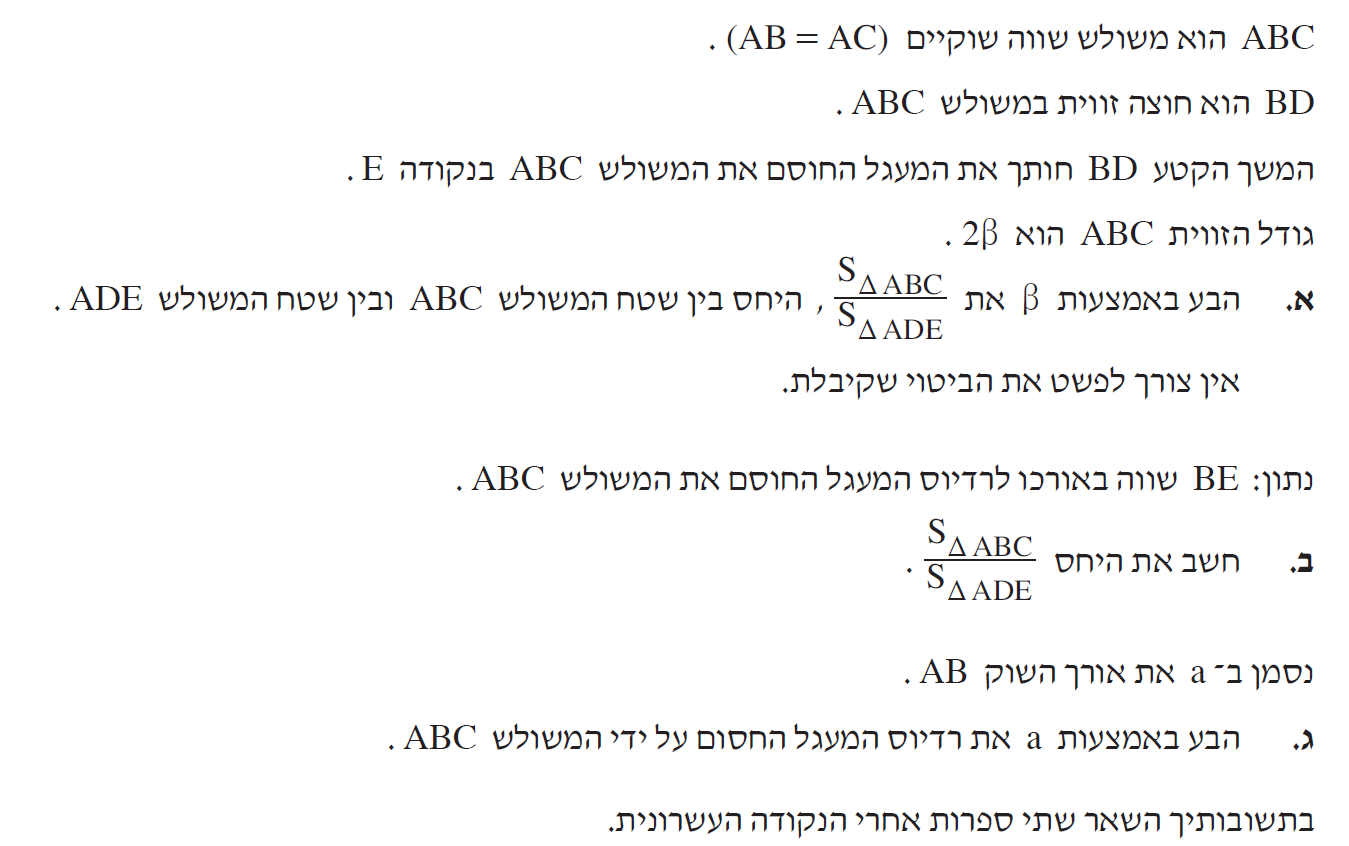
\includegraphics[width=\textwidth]{summer-2018b-5}
\end{center}

להלן התרשים עם הזוויות הנתונות ב-%
$B,C$
ולאחר חישוב הזוויות האחרות לפי סכום של זוויות של משולש. כמו כן,
$\angle EAC=\angle EBC=\beta$,
$\angle AEB=\angle ACB=2\beta$,
כי הן נשענות על אותן קשתות. התרשים נראה דחוס, אבל ציירתי אותו לפי הזוויות המתקבלות במהלך הפתרון.
\begin{center}
\selectlanguage{english}
\begin{tikzpicture}[scale=1.4]
\clip(-5mm,-5mm) rectangle +(11,2.8);
\coordinate (B) at (0,0);
\coordinate (C) at (10,0);
\path[name path=ba] (B) -- +(20:6);
\path[name path=ca] (C) -- +(160:6);
\path[name intersections={of=ca and ba,by={A}}];
\draw[thick] (A) -- node[above,xshift=24pt,yshift=10pt] {$a$} (B) -- (C) -- cycle;
\path[name path=bd] (B) -- +(10:8.5);
\tkzCircumCenter(A,B,C)\tkzGetPoint{O}
\node[draw,very thick,dotted,circle through=(A),name path=circle] (circle) at (O) {};
\path[name intersections={of=bd and ca,by={D}}];
\path[name intersections={of=bd and circle,by={E}}];
\fill (A) node[above] {$A$} circle(1.5pt);
\fill (B) node[left,xshift=-4pt] {$B$} node[above right,xshift=85pt,yshift=-1pt] {$\beta$} node[above right,xshift=85pt,yshift=16pt] {$\beta$} circle(1.5pt);
\fill (C) node[right,xshift=4pt] {$C$} node[above left,xshift=-42pt,yshift=-1pt] {$2\beta$} circle(1.5pt);
\fill (D) node[above,yshift=-2pt] {$D$} node[left,xshift=-20pt,yshift=1pt] {$3\beta$} node[below,xshift=-3,yshift=-6pt] {$180\!-\!3\beta$} circle(1.5pt);
\fill (E) node[above] {$E$} circle(1.5pt);
\draw[thick] (B) -- (D) -- (E) -- (A);
\node at ($(E)+(28pt,0pt)$) {$2\beta$};
\draw[->,thick] ($(E)+(20pt,0pt)$) -- +(-38pt,0);
\node at ($(A)+(28pt,6pt)$) {$\beta$};
\draw[->,thick] ($(A)+(27pt,1pt)$) -- +(0,-10pt);
\node at ($(A)+(-28pt,6pt)$) {$180\!-\!4\beta$};
\draw[->,thick] ($(A)+(-27pt,1pt)$) -- +(27pt,-6pt);
\end{tikzpicture}
\end{center}

\textbf{סעיף א}


$\triangle ABC$
משולש שוקיים ולכן מייד יש לנו:
\[
S_{\triangle ABC}=\frac{1}{2}\cdot a\cdot a \cdot \sin (180\!-\!4\beta)=\frac{a^2}{2}\sin 4\beta\,.
\]
כדי שהיחס יהיה ביטוי ב-%
$\beta$
בלבד, עלינו למצוא ביטוי ל-%
$S_{\triangle ADE}$
כדי ש-%
$a^2$
יצטמצם.

\np

נחפש משולשים כדי לבטא 
$AE,AD$
כביטויים ב-%
$a,\beta$
כדי ש-%
$a^2$
יצטמצם. ב-%
$\triangle ABD,\triangle ABE$
צלע אחד הוא באורך 
$a$
וצלע שני באורך
$AD,AE$.
לפי חוק הסינוסים:
\erh{14pt}
\begin{equationarray*}{rcl}
\frac{AE}{\sin \beta}&=&\frac{a}{\sin 2\beta}\\
AE&=&\frac{a\sin\beta}{\sin 2\beta}\\
\frac{AD}{\sin \beta}&=&\frac{a}{\sin 3\beta}\\
AD&=&\frac{a\sin\beta}{\sin 3\beta}\\
S_{\triangle ADE}&=&\frac{1}{2}\cdot \frac{a\sin \beta}{\sin 2\beta}\cdot\frac{a\sin\beta}{\sin 3\beta}\cdot \sin \beta\\
&=&\frac{a^2}{2}\cdot \frac{\sin^3 \beta}{\sin 2\beta\sin 3\beta}\\
\frac{S_{\triangle ABC}}{S_{\triangle ADE}}&=&\frac{\sin 4\beta\sin 2\beta\sin 3\beta}{\sin^3\beta}\,.
\end{equationarray*}

אפשרות אחרת היא לאחר חישוב 
$AE$
או
$AD$,
להשתמש בחוק הסינוסים על המשולש 
$\triangle ADE$
כדי לחשב  את השני.


\textbf{סעיף ב}

נשתמש בחוק הסינוסים על 
$\triangle ABE$
עם צלע 
$BE$,
ומ-%
$R=BE$
הרדיוס יצטמצם:
\erh{12pt}
\begin{equationarray*}{rcl}
2R&=&\frac{BE}{\sin(180\!-\!4\beta+\beta)}=\frac{BE}{\sin 3\beta}=\frac{R}{\sin 3\beta}\\
2\sin 3\beta&=&1\\
3\beta&=&30^\circ\\
\beta&=&10^\circ\,.
\end{equationarray*}
נכון שגם
$\sin 3\cdot 50 = \frac{1}{2}$,
אבל לא ייתכן שלמשולש שתי זוויות של 
$2\cdot 50=100$.

עם ערכו של 
$\beta$
נוכל לחשב את יחס השטחים:
\[
\frac{S_{\triangle ABC}}{S_{\triangle ADE}}=\frac{\sin 4\beta\sin 2\beta\sin 3\beta}{\sin^3\beta}=\frac{\sin 40\sin 20\sin 30}{\sin^3 10}=20.99^\circ\,.
\]

\np

\textbf{סעיף ג}

לפי משפט
$6$
"במשולש שווה שוקיים , חוצה זווית הראש, התיכון לבסיס והגובה לבסיס מתלכדים", כך שחוצה הזווית 
$\angle BAC$
ניצב ל-%
$BC$
בנקודה
$F$.
לפי משפט
$49$
"שלושת חוצי הזוויות של משולש נחתכים בנקודה אחת, שהיא מרכז המעגל החסום במשולש", הנקודה המסומנת 
$M$
בתרשים היא מרכז המעגל החסום.

\begin{center}
\selectlanguage{english}
\begin{tikzpicture}[scale=1.3]
\coordinate (B) at (0,0);
\coordinate (C) at (10,0);
\path[name path=ba] (B) -- +(20:6);
\path[name path=ca] (C) -- +(160:6);
\path[name intersections={of=ca and ba,by={A}}];
\draw[thick] (A) -- node[above,xshift=24pt,yshift=10pt] {$a$} (B) -- (C) -- cycle;
\path[name path=bd] (B) -- +(10:8.5);
\path[name intersections={of=bd and ca,by={D}}];
\fill (A) node[above] {$A$} circle(1.5pt);
\fill (B) node[left,xshift=-4pt] {$B$} node[above right,xshift=85pt,yshift=-1pt] {$\beta$} node[above right,xshift=85pt,yshift=16pt] {$\beta$} circle(1.5pt);
\fill (C) node[right,xshift=4pt] {$C$} circle(1.5pt);
\draw[thick] (B) -- (D);
\node at ($(A)+(-28pt,6pt)$) {$90\!-\!2\beta$};
\draw[->,thick] ($(A)+(-27pt,1pt)$) -- +(20pt,-10pt);
\coordinate (F) at ($(B)!(A)!(C)$);
\draw[rotate=90] (F) rectangle +(7pt,7pt);
\draw[thick,dashed,name path=altitude] (A) -- (F);
\path[name intersections={of=bd and altitude,by={M}}];
\fill (F) node[below] {$F$} circle(1.5pt);
\fill (M) node[above right] {$M$} circle(1.5pt);
\path (B) -- node[below] {$b$} (F);
\path (M) -- node[right] {$r$} (F);
\node[draw,very thick,dotted,circle through=(F),name path=circle] (circle) at (M) {};
\end{tikzpicture}
\end{center}
נשאר רק להשתמש בהגדרות של הפונקציות הטריגונומטריות. ב-%
$\triangle ABF$:
\erh{10pt}
\begin{equationarray*}{rcl}
\sin(90\!-\!2\beta)&=&\frac{b}{a}\\
b&=&a\cos 2\beta\,.
\end{equationarray*}

\vspace{-4ex}
ב-%
$\triangle BMF$:
\vspace{-4ex}
\erh{10pt}
\begin{equationarray*}{rcl}
\tan\beta&=&\frac{r}{b}\\
r&=&a\cos 2\beta\tan\beta\\
&=&a\cos 20\tan 10=0.1657a\,.
\end{equationarray*}

%%%%%%%%%%%%%%%%%%%%%%%%%%%%%%%%%%%%%%%%%%%%%%%%%%%%%%%%%%%%%%

\np

\section{קיץ תשע"ח מועד א}

\begin{center}
\selectlanguage{english}
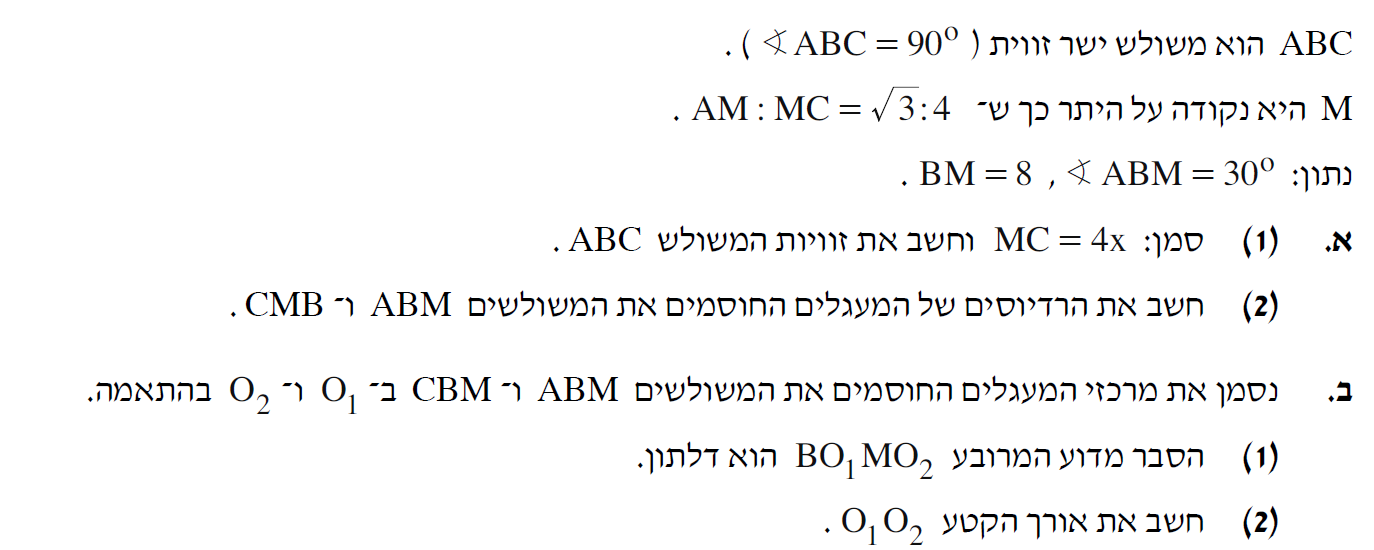
\includegraphics[width=\textwidth]{summer-2018a-5}
\end{center}
נסמן
$\angle BAM=\alpha, \angle BCM=90\!-\!\alpha$.

\vspace{-1ex}

\begin{center}
\selectlanguage{english}
\begin{tikzpicture}%[scale=1.1]
\coordinate (C) at (0,0);
\coordinate (B) at (7,0);
\path[name path=ca] (C) -- +(36:9);
\path[name path=ba] (B) -- +(90:5.5);
\path[name intersections={of=ca and ba,by={A}}];
\draw[thick] (A) -- (B) -- (C) -- cycle;
\coordinate (M) at ($(C)!{4/(sqrt(3)+4)}!(A)$);
\fill (C) node[left] {$C$} node[above right,xshift=18pt] {$90\!-\!\alpha$}circle(1.5pt);
\fill (B) node[right] {$B$} node[above left,xshift=-10pt] {$60$} node[above left,xshift=2pt,yshift=24pt] {$30$} circle(1.5pt);
\fill (A) node[right] {$A$} node[below left,xshift=2pt,yshift=-8pt] {$\alpha$} circle(1.5pt);
\fill (M) node[above left] {$M$} circle(1.5pt);
\draw[thick] (B) -- node[left,xshift=-3pt] {$8$} (M);
\path (C) -- node[above,xshift=-4pt] {$4x$} (M) -- node[above,xshift=-6pt] {$\sqrt{3}x$} (A);
\draw[rotate=90] (B) rectangle +(8pt,8pt);
\end{tikzpicture}
\end{center}

\vspace{-1ex}

\textbf{סעיף א}

$(1)$
לשני המשולשים 
$\triangle ABM,\triangle CMB$
צלע עם הנעלם
$x$,
זווית ידועה אחת, וזווית שנייה עם הנעלם 
$\alpha$.
מחוק הסינוסים נקבל שתי משוואות עם שני הנעלמים שאפשר לפתור אתכדי לקבל משוואה אחת עם הנעלם
$\alpha$
בלבד:
\erh{14pt}
\begin{equationarray*}{rcl}
\frac{\sqrt{3}x}{\sin 30}&=&\frac{8}{\sin\alpha}\\
x&=&\frac{8\sin 30}{\sqrt{3}x\sin\alpha}\\
\frac{4x}{\sin 60}&=&\frac{8}{\sin (90\!-\!\alpha)}\\
x&=&\frac{8\sin 60}{4x\cos\alpha}
\end{equationarray*}

\np

\erh{10pt}
\begin{equationarray*}{rcl}
\frac{1}{2\sqrt{3}\sin\alpha}&=&\frac{\sqrt{3}}{4\cdot 2\cos \alpha}\\
\tan \alpha&=&\frac{4}{3}\,.
\end{equationarray*}
לכן,
$\angle BAC=\alpha = 53.13$,
ולא נשכח לרשום גם 
$\angle BCA=90\!-\!\alpha=36.87$.


$(2)$
לפי חוק הסינוסים עבור 
$\triangle ABM$, $\triangle CMB$:
\erh{8pt}
\begin{equationarray*}{rcl}
2R_1&=&\frac{8}{\sin\alpha}\\
R_1&=&5\\
2R_2&=&\frac{8}{\sin(90\!-\!\alpha)}\\
R_2&=&20/3\,.
\end{equationarray*}

\vspace{-3ex}

\textbf{סעיף ב}

$(1)$
נצייר התרשים חדש עם המעגלים החוסמים. ניתן לראות ש-%
$O_1M=O_1B$
כי הם רדיוסים של המעגל החוסם את
$\triangle ABM$,
ו-%
$O_2M=O_2B$
כי הם רדיוסים של המעגל החוסם את
$\triangle CBM$.
לפי ההגדרה מרובע עם שני זוגות של צלעות שכנים שהם שווים הוא דלתון.
\begin{center}
\selectlanguage{english}
\begin{tikzpicture}%[scale=1.1]
\clip (-6mm,-5mm) rectangle +(11,6);
\coordinate (C) at (0,0);
\coordinate (B) at (7,0);
\path[name path=ca] (C) -- +(36:9);
\path[name path=ba] (B) -- +(90:5.5);
\path[name intersections={of=ca and ba,by={A}}];
\draw[thick] (A) -- (B) -- (C) -- cycle;
\coordinate (M) at ($(C)!{4/(sqrt(3)+4)}!(A)$);
\fill (C) node[left] {$C$} circle(1.5pt);
\fill (B) node[right] {$B$} circle(1.5pt);
\fill (A) node[right] {$A$} circle(1.5pt);
\fill (M) node[above left] {$M$} circle(1.5pt);
\draw[thick] (B) -- (M);
\tkzCircumCenter(A,B,M)\tkzGetPoint{O1}
\tkzCircumCenter(C,B,M)\tkzGetPoint{O2}
\fill (O1) node[above right] {$O_1$} circle(1.5pt);
\fill (O2) node[above left] {$O_2$} circle(1.5pt);
\node [draw,thick,dotted,circle through=(M)] (circle) at (O1) {};
\node [draw,thick,dotted,circle through=(M)] (circle) at (O2) {};
\draw[thick] (O1) -- node[right] {$R_1$} (B) -- node[below,yshift=-3pt] {$R_2$} (O2) -- node[left] {$R_2$} (M) -- node[above] {$R_1$} cycle;
\draw[thick,name path=diagonal1] (O1) -- (O2);
\path[name path=diagonal2] (M) -- (B);
\path[name intersections={of=diagonal1 and diagonal2,by={E}}];
\fill (E) node[left,xshift=-3pt,yshift=2pt] {$E$} circle(1.5pt);
\draw[rotate=32] (E) rectangle +(7pt,7pt);
\path (M) -- node[left] {$4$} (E) -- node[left,xshift=-3pt,yshift=4pt] {$4$} (B);
\end{tikzpicture}
\end{center}

$(2)$
לפי משפט
$21$
"האלכסון הראשי בדלתון חוצה את זוויות הראש, חוצה את האלכסון השני ומאונך לו", 
$MB\perp O_1O_2$
וחוצה אותו. את האורך של
$O_1O_2$
ניתן לחשב כסכום האורכים ממרכזי המעגלים ועד לנקודת החיתוך של האלכסונים. נשמתמש במשפט פיתגורס:
\erh{16pt}
\begin{equationarray*}{rcl}
O_1O_2=O_1E+O_2E&=&\sqrt{R_1^2-16} + \sqrt{R_2^2-16}\\
&=&\sqrt{5^2-16} + \sqrt{\left(\frac{20}{3}\right)^2-16}\\
&=&3+\frac{16}{3}=\frac{25}{3}\,.
\end{equationarray*}

%%%%%%%%%%%%%%%%%%%%%%%%%%%%%%%%%%%%%%%%%%%%%%%%%%%%%%%%%%%%%%

\np


\section{חורף תשע"ח}

\begin{center}
\selectlanguage{english}
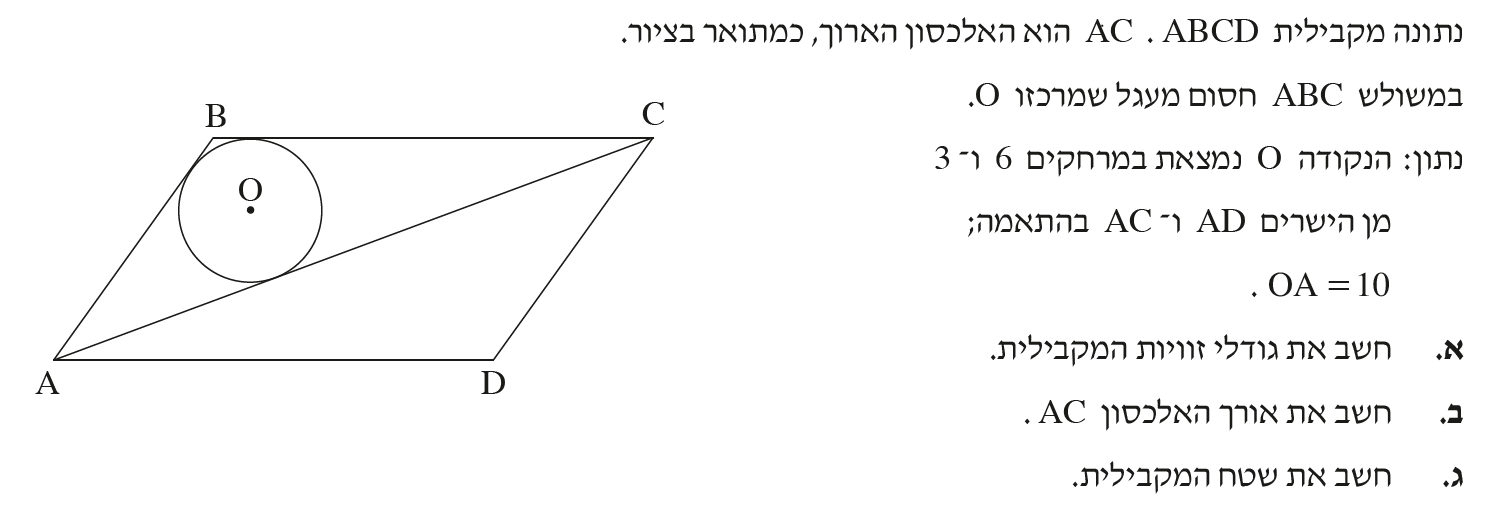
\includegraphics[width=\textwidth]{winter-2018-5}
\end{center}

\vspace{-1ex}

$E,F$
הן נקודות המפגש של האנכים מ-%
$O$
עם 
$AC,AD$.
לפי משפט
$49$
"שלושת חוצי הזוויות של משולש נחתכים בנקודה אחת, שהיא מרכז המעגל החסום במשולש", 
$AO,CO$
הם חוצי הזוויות
$BAC,BCA$,
בהתאמה. המונח "חוצה זוויות" נתפס לי בראש ו"פתרתי" את הבעיה תוך הנחה שאלכסון של מקבילית חוצה את הזווית:
$\angle BAC=\angle CAD$.
כמובן שזה נכון רק עבור מעוין.

נסמן את הזוויות בנקודה
$A$
עבור המשולשים ישר-זווית
$\triangle AOE, \triangle AOF$
שנוצרו על ידי האנכים:
$\alpha=\angle OAE,\beta=\angle OAF$.

\vspace{-2ex}

\begin{center}
\selectlanguage{english}
\begin{tikzpicture}%[scale=1.1]
\clip (-12mm,-5.5mm) rectangle +(12.5,5);
\coordinate (A) at (0,0);
\coordinate (D) at (8,0);
\coordinate (B) at (54:4.5);
\coordinate (C) at ($(D)+(54:4.5)$);
\fill (A) node[below] {$A$} circle(1.5pt);
\fill (B) node[above] {$B$} circle(1.5pt);
\fill (C) node[above] {$C$} circle(1.5pt);
\fill (D) node[below] {$D$} circle(1.5pt);
\draw[thick] (D) -- (A) -- (B) -- (C) -- cycle;
\draw[thick] (A) -- (C);
\tkzInCenter(A,B,C)\tkzGetPoint{O}
\fill (O) node[above] {$O$} circle(1.5pt);
\node[draw,thick,circle through=($(B)!(O)!(C)$),name path=circle] at (O) {};
\draw[thick,dashed] (A) -- node[left,near end,xshift=10pt,yshift=12pt] {$10$} (O) -- (C);
\coordinate (E) at ($(A)!(O)!(C)$);
\coordinate (F) at ($(A)!(O)!(D)$);
\fill (E) node[below right] {$E$} circle(1.5pt);
\fill (F) node[below] {$F$} circle(1.5pt);
\draw[thick,dashed] (E) -- node[right,near end] {$3$} (O) -- node[right,near end] {$6$} (F);
\draw[rotate=19] (E) rectangle +(7pt,7pt);
\draw (F) rectangle +(7pt,7pt);
\draw[thick] ($(A)+(20mm,0)$) arc[start angle=0,end angle=37,radius=20mm];
\node[right,xshift=54pt,yshift=12pt] at (A) {$\beta$};
\node[above right,xshift=34pt,yshift=14pt] at (A) {$\alpha$};
\node[above right,xshift=28pt,yshift=28pt] at (A) {$\alpha$};
\node at (-2mm,2.5) {$\angle OAF=\beta$};
\end{tikzpicture}
\end{center}

\vspace{-2ex}

\textbf{סעיף א}

לפי התרשים
$\angle BAD=\alpha+\beta$.
נחשב
$\alpha,\beta$
מהפונקציות הטריגונומטריות במשולשים ישר-זווית:
\erh{12pt}
\begin{equationarray*}{rcl}
\sin \alpha &=& 3/10\\
\alpha &=& 17.46\\
\sin \beta &=& 6/10\\
\beta &=& 36.87\\
\angle BCD =\angle BAD&=& \alpha+\beta=54.33\\
\angle ABC =\angle ADC&=& \frac{360-2(\alpha+\beta)}{2}=125.67\,.
\end{equationarray*}

\np


\textbf{סעיף ב}

האלכסון
$AC$
הוא צלע של
$\triangle ABC$
והזוויות שלו ידועים, אבל אי-אפשר להשתמש בחוק הסינוסים כי אורכי הצלעות לא ידועים. מהתרשים רואים שהאלכסון מורכב משני קטעי קו
$AE,EC$
שהם צלעות של משולשים ישר-זווית
$\triangle AOE, \triangle COE$.
$AE$
מתקבל ממשפט פיתגורס:
\[
AE = \sqrt{10^2-3^2}=9.54\,.
\]
נשתמש בחוק הסינוסים ב-%
$\triangle COE$
)ונימנע מהפיתוי לקבוע ש-%
$\angle OCE=\alpha$(.
לפי זוויות מתחלפות במקבילית
$\angle BCA=\angle CAD=\beta-\alpha$
ו:

\vspace{-2ex}

\erh{12pt}
\begin{equationarray*}{rcl}
\angle OCE=\frac{\angle BCA}{2}&=&\frac{\beta-\alpha}{2}\\
&=&\frac{36.87-17.46}{2}=9.71\\
\angle COE &=& 180-90-\angle OCE=80.29\\
\frac{EC}{\sin 80.29}&=& \frac{3}{\sin 9.71}\\
EC&=&17.54\\
AC=AE+EC&=&9.54+17.54=27.08\,.
\end{equationarray*}

\vspace{-2ex}

\textbf{סעיף ג}

שטח של מקבילית הוא הבסיס כפול הגובה:

\begin{center}
\selectlanguage{english}
\begin{tikzpicture}[scale=.7]
\coordinate (A) at (0,0);
\coordinate (B) at (54:4.5);
\coordinate (D) at (8,0);
\coordinate (C) at ($(D)+(54:4.5)$);
\fill (A) node[below] {$A$} node[above right,xshift=46pt,yshift=0pt] {$\beta-\alpha$} node[above right,xshift=16pt,yshift=10pt] {$2\alpha$} circle(1.5pt);
\fill (B) node[above] {$B$} circle(1.5pt);
\fill (C) node[above] {$C$} circle(1.5pt);
\fill (D) node[below] {$D$} circle(1.5pt);
\draw[thick] (D) -- node[below] {$b$} (A) -- node[above,yshift=2pt] {$27.08$} (C) -- cycle;
\draw[thick] (A) -- (B) -- (C);
\coordinate (H) at ($(A)!(C)!(D)$);
\fill (H) node[below] {$H$} circle(1.5pt);
\draw[rotate=90] (H) rectangle +(10pt,10pt);
\draw[thick,dashed] (D) -- (H) -- node[right] {$h$} (C);
\node[above left,xshift=-2pt,yshift=2pt] at (D) {$125.67$};
\node[below left,xshift=-16pt,yshift=-12pt] at (C) {$2\alpha$};
\end{tikzpicture}
\end{center}

\vspace{-4ex}

\erh{12pt}
\begin{equationarray*}{rcl}
\frac{b}{\sin 2\alpha}&=&\frac{27.08}{\sin 125.67}\\
b&=&19.08\\
\sin (\beta-\alpha) &=& \frac{h}{27.08}\\
h&=&9\\
S_{ABCD}=bh&=&171.71\,.
\end{equationarray*}

\vspace{-2ex}


אפשרות אחרת היא להשתמש בנוסחה הטריגונומטרית כדי לחשב 
$S_{\triangle ABC}$
ולהכפיל בשניים.

%%%%%%%%%%%%%%%%%%%%%%%%%%%%%%%%%%%%%%%%%%%%%%%%%%%%%%%%%%%%%%

\np

\section{קיץ תשע"ז מועד ב}

\begin{center}
\selectlanguage{english}
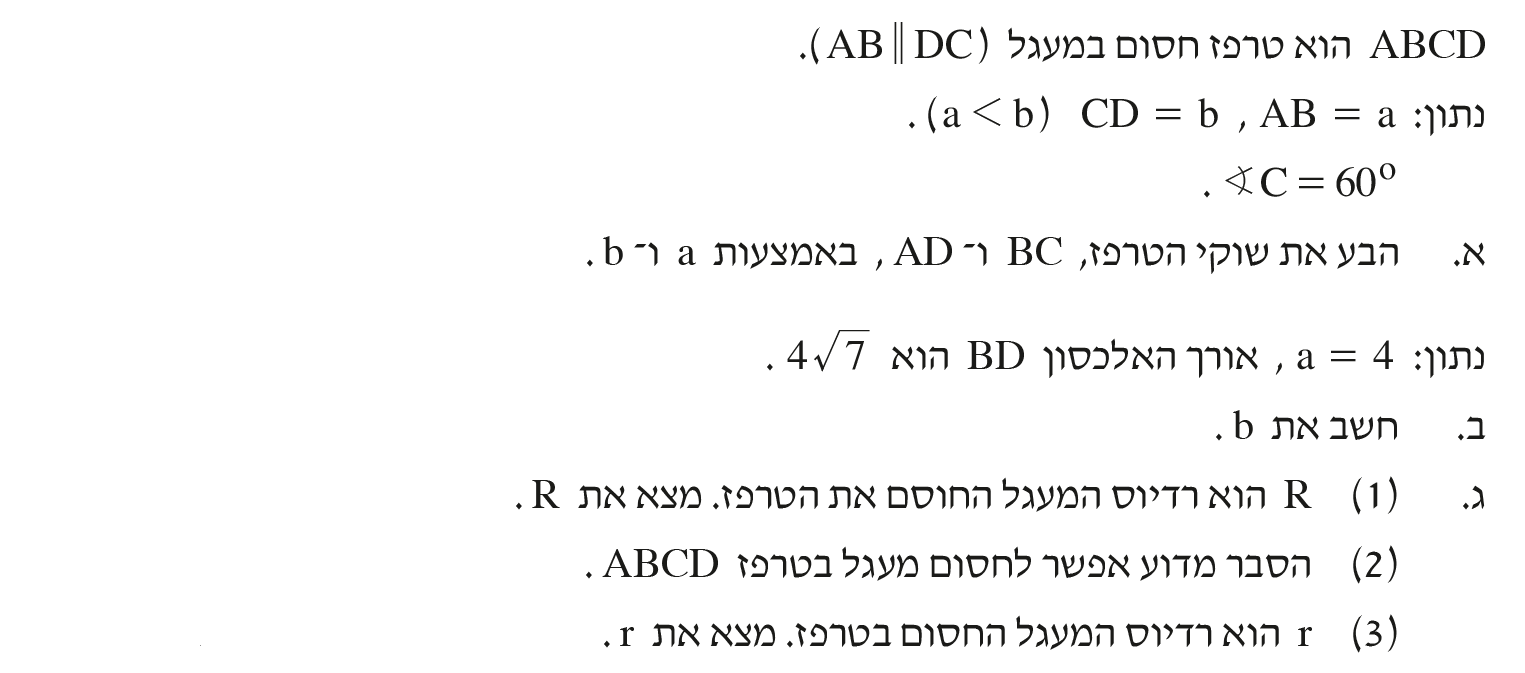
\includegraphics[width=\textwidth]{summer-2017b-5}
\end{center}

\vspace{-1ex}

\textbf{סעיף א}


לפי משפט
$56$
"ניתן לחסום מרובע במעגל אם ורק אם סכום זוג זוויות נגדיות שווה ל-%
$180$",
ולכן
$\angle DAB=120$.
נוריד גבהים מ-%
$A,B$
ל-%
$CD$
החותחכים אותו ב-%
$E,F$.
$\triangle AED,\triangle BFC$
הם משולשים ישר-זווית. בתרשים השלמנו את הזוויות במשולשים ל-%
$180$.
לפי משפט
$40$
"טרפז בו הזוויות שליד אותו בסיס שוות זו לזו הוא טרפז שווה שוקיים", 
$ABCD$
שווה שוקיים.
\begin{center}
\selectlanguage{english}
\begin{tikzpicture}[scale=1.1]
\clip (-.5,-.5) rectangle +(9,4.25);
\draw[thick] (0,0) coordinate (D) node[below left] {$D$} -- node[below] {$b$} (8,0) coordinate (C) node[below right] {$C$};
\fill (C) node[above left,xshift=-4pt] {$60$} circle(1.5pt);
\fill (D) node[above right,xshift=4pt] {$60$} circle(1.5pt);
\path[name path=s1] (D) -- +(60:4);
\path[name path=s2] (C) -- +(120:4);
\path[name path=top] (1,3) -- (7,3);
\path[name intersections={of=s1 and top,by={A}}];
\path[name intersections={of=s2 and top,by={B}}];
\fill (A) node[above left] {$A$} node[below right] {$90$} node[below,xshift=-8pt,yshift=-22pt] {$30$}  circle(1.5pt);
\fill (B) node[above right] {$B$} node[below left] {$90$}  node[below,xshift=8pt,yshift=-22pt] {$30$} circle(1.5pt);
\draw[thick] (D) -- node[left] {$s$} (A) -- node[above] {$a$} (B) -- node[right] {$s$} (C);
\tkzCircumCenter(A,B,C)\tkzGetPoint{O}
\tkzDrawCircle[thick,dotted,name path=circle](O,A)
\coordinate (E) at (D-|A);
\fill (E) node[below] {$E$} circle(1.5pt);
\draw[thick,dashed] (A) -- (E);
\draw (E) rectangle +(8pt,8pt);
\coordinate (F) at (D-|B);
\fill (F) node[below] {$F$} circle(1.5pt);
\draw[thick,dashed] (B) -- (F);
\draw[rotate=90] (F) rectangle +(8pt,8pt);
\draw[dashed] (A) -- node[below,xshift=-4pt] {$c$} (C);
\end{tikzpicture}
\end{center}
$AE=BF$
כך ש-%
$\triangle AED\cong\triangle BFC$.
מכאן:

\vspace{-2ex}

\erh{6pt}
\begin{equationarray*}{rcl}
\cos 60 &=& \frac{(b-a)/2}{s}=\frac{1}{2}\\
s&=&b-a\,.
\end{equationarray*}

\vspace{-4ex}

פתרון אחר משתמש בחוק הקוסינוסים על 
$\triangle ACD,\triangle ACB$.
נסמן ב-%
$c$
את אורך האלכסון
$AC$.

\vspace{-2ex}

\erh{2pt}
\begin{equationarray*}{rcl}
c^2 &=& s^2+b^2-2sb\cos 60\\
&=& s^2-sb+b^2\\
c^2 &=& s^2+a^2-2sa\cos 120\\
&=& s^2+sa+a^2
\end{equationarray*}
\vspace{-3ex}

נשווה את שתי הנוסחאות ל-%
$c^2$
ונפתור עבור 
$s$:

\np

\erh{2pt}
\begin{equationarray*}{rcl}
s(b+a)&=&b^2-a^2=(b+a)(b-a)\\
s&=&b-a\,.
\end{equationarray*}

\vspace{-4ex}

\textbf{סעיף ב}

שקלתי להשתמש בחוק הסינוסים במשלוש
$\triangle ADB$:
פעם אחת לחשב 
$\angle ADB$
ופעם שנייה לחשב את
$s$.
עדיף להשתמש בחוק הקוסינוסים ב-%
$\triangle ADB$
כי אנו יודעים ש-%
$s=b-a=b-4$:
\erh{3pt}
\begin{equationarray*}{rcl}
(4\sqrt{7})^2&=&4^2+(b-4)^2-2\cdot 4\cdot (b-4)\cdot \cos 120\\
b^2-4b-96&=&0\\
(b-12)(b+8)&=&0\\
b&=&12\,.
\end{equationarray*}

\vspace{-2ex}

\begin{center}
\selectlanguage{english}
\begin{tikzpicture}[scale=1.1]
\clip (-.5,-.5) rectangle +(9,4.25);
\draw[thick] (0,0) coordinate (D) node[below left] {$D$} -- node[above] {$b$} (8,0) coordinate (C) node[below right] {$C$};
\fill (C) node[above left,xshift=-4pt] {$60$} circle(1.5pt);
\fill (D) circle(1.5pt);
\path[name path=s1] (D) -- +(60:4);
\path[name path=s2] (C) -- +(120:4);
\path[name path=top] (1,3) -- (7,3);
\path[name intersections={of=s1 and top,by={A}}];
\path[name intersections={of=s2 and top,by={B}}];
\fill (A) node[above left] {$A$} node[below right] {$120$} circle(1.5pt);
\fill (B) node[above right] {$B$} circle(1.5pt);
\draw[thick] (D) -- node[left,xshift=-14pt] {$b-4$} (A) -- node[above] {$4$} (B) -- node[right,xshift=14pt] {$b-4$} (C);
\tkzCircumCenter(A,B,C)\tkzGetPoint{O}
\tkzDrawCircle[thick,dotted,name path=circle](O,A)
\fill (O) circle(3pt);
\coordinate (E) at (D-|A);
\coordinate (F) at (D-|B);
\fill (F) node[below] {$F$} circle(1.5pt);
\draw[thick,dashed] (B) -- node[left] {$2r$} (F);
\draw[rotate=90] (F) rectangle +(8pt,8pt);
\draw[thick,dashed] (B) -- node[below] {$4\sqrt{7}$} (D);
\end{tikzpicture}
\end{center}


\textbf{סעיף ג}

$(1)$
שימו לב שהאלכסון
$BD$
הוא 
\textbf{לא}
הקוטר של המעגל החוסם שמסומן בנקודה השחורה הגדולה. לפי חוק הסינוסים ב-%
$\triangle ADB$:
\[
R = \frac{4\sqrt{7}}{2\sin 120} = \frac{4\sqrt{7}}{\sqrt{3}}=6.11\,.
\]

\vspace{-1ex}

$(2)$
לפי משפט
$57$,
"מרובע קמור חוסם מעגל אם ורק אם סכום שתי צלעות נגדיות שווה לסכום שתי הצלעות הנגדיות האחרות":

\vspace{-4ex}

\erh{3pt}
\begin{equationarray*}{rcl}
a+b&\stackrel{?}{=}&s+s\\
a+b&\stackrel{?}{=}&(b-a)+(b-a)\\
3a&\stackrel{?}{=}&b\\
3\cdot 4&=&12\,.
\end{equationarray*}

\vspace{-4ex}

$(3)$
$AB,CD$
הם משיקים מקבילים למעגל החסום, ולכן
$BF=2r$:
\erh{14pt}
\begin{equationarray*}{rcl}
\sin 60 &=& \frac{2r}{s}=\frac{2r}{b-a}=\frac{2r}{8}\\
r&=&\frac{1}{2}\cdot\frac{\sqrt{3}}{2}\cdot 8 = 2\sqrt{3}=3.464\,.
\end{equationarray*}

%%%%%%%%%%%%%%%%%%%%%%%%%%%%%%%%%%%%%%%%%%%%%%%%%%%%%%%%%%%%%%


\np


\section{קיץ תשע"ז מועד א}

\begin{center}
\selectlanguage{english}
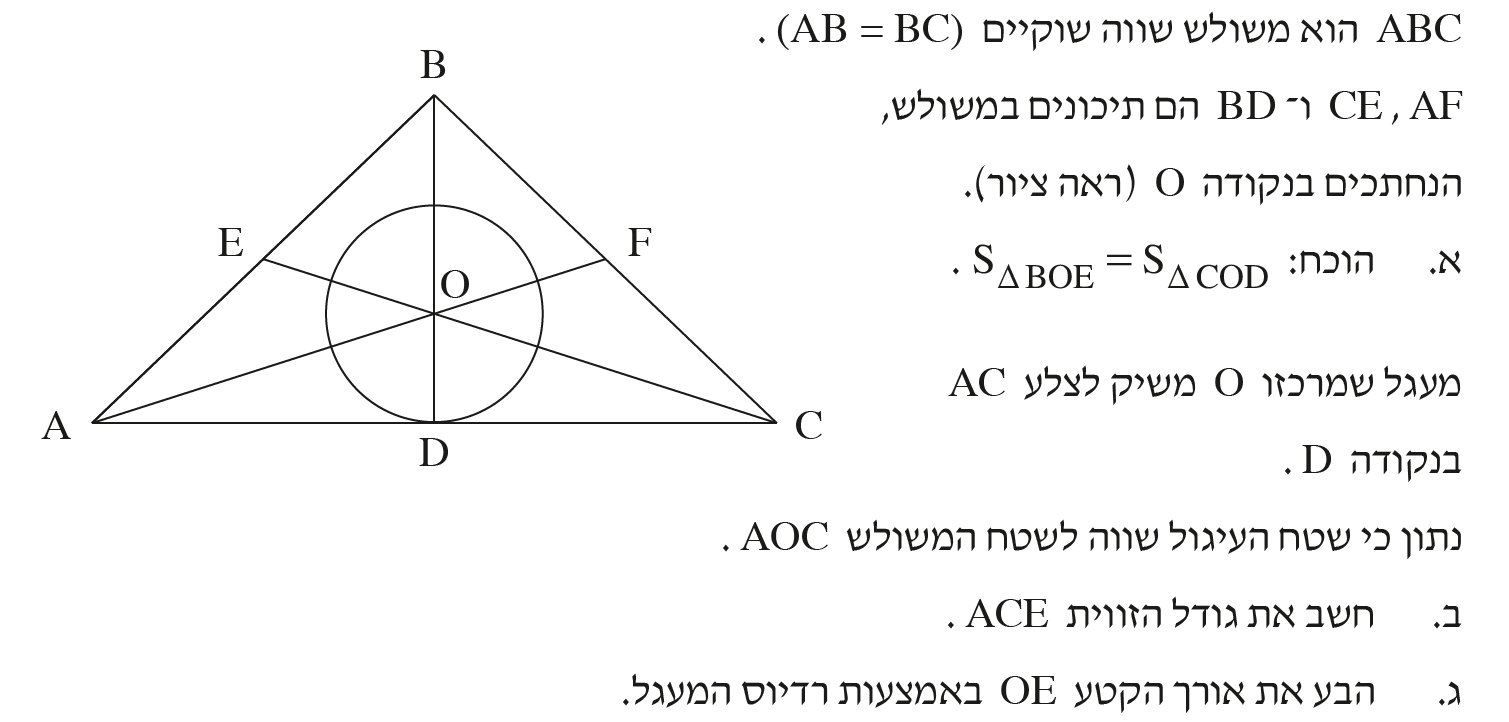
\includegraphics[width=\textwidth]{summer-2017a-5}
\end{center}

\vspace{-2ex}

\textbf{סעיף א}

נסמן בתרשים לפי: 
$\triangle ABC$
שווה שוקיים,
$AF,BD,CF$
תיכונים. משפט
$46$
"נקודת חיתוך התיכונים מחלקת כל תיכון ביחס 
$2\!:\!1$".
$AF=CE$
כי
$\triangle CAF\cong \triangle ACE$
לפי צ.ז.צ. כי 
$\triangle ABC$
שווה-שוקיים.

\vspace{-1ex}

\begin{center}
\selectlanguage{english}
\begin{tikzpicture}[scale=1.1]
\draw[thick] (0,0) coordinate (A) node[left] {$A$} -- (8,0) coordinate (C) node[right] {$C$} -- (4,4.5) coordinate (B) node[above] {$B$} -- cycle;
\fill (A) circle(1.5pt);
\fill (B) circle(1.5pt);
\fill (C) circle(1.5pt);
\coordinate (D) at ($(A)!.5!(C)$);
\coordinate (E) at ($(A)!.5!(B)$);
\coordinate (F) at ($(C)!.5!(B)$);
\fill (D) node[below] {$D$} circle(1.5pt);
\fill (E) node[left,xshift=-2pt,yshift=2pt]  {$E$} circle(1.5pt);
\fill (F) node[right,xshift=2pt,yshift=2pt] {$F$} circle(1.5pt);
\draw (D) rectangle +(8pt,8pt);
\draw[thick,name path=af] (A) -- (F);
\draw[thick,name path=ce] (C) -- (E);
\draw[thick,name path=bd] (B) -- (D);
\path[name intersections={of=af and ce,by={O}}];
\fill (O) node[above right,yshift=2pt] {$O$} node[above left,xshift=2pt,yshift=2pt] {$\alpha$} node[below right,xshift=-2pt,yshift=-2pt] {$\alpha$} circle(1.5pt);
\path (A) -- node[below] {$a/2$} (D) -- node[below] {$a/2$} (C);
\path (A) -- node[left] {$b/2$} (E) -- node[left] {$b/2$} (B);
\path (C) -- node[right] {$b/2$} (F) -- node[right] {$b/2$} (B);
\path (B) -- node[right] {$2r$} (O) -- node[right] {$r$} (D);
\path (A) -- node[above] {$2c$} (O) -- node[below] {$c$} (F);
\path (C) -- node[above] {$2c$} (O) -- node[below] {$c$} (E);
\draw[thick,dashed,name path=ef] (E) -- (F);
\path[name intersections={of=ef and bd,by={G}}];
\fill (G) node[above left] {$G$} circle(1.5pt);
\draw (G) rectangle +(8pt,8pt);
\end{tikzpicture}
\end{center}

\vspace{-1ex}


נשתמש במשפט
$91$
"משפט תאלס המורחב: ישר המקביל לאחת מצלעות המשולש חותך את שתי הצלעות האחרות או את המשכיהן בקטעים פרופורציוניים", כך ש-%
$EF=\displaystyle\frac{AC}{2}=\frac{a}{2}$.
$\triangle EBF$
גם הוא שווה-שוקיים, ולכן,
$EG=\displaystyle\frac{EF}{2}=\frac{a}{4}$.

\vspace{-1ex}

\erh{16pt}
\begin{equationarray*}{rcl}
S_{BOE}&=&\frac{1}{2}\cdot \frac{a}{4}\cdot BG+\frac{1}{2}\cdot \frac{a}{4}\cdot GO =\frac{a}{8}(BG+GO)=\frac{a}{8}\cdot 2r= \frac{ar}{4}\\
S_{COD} &=& \frac{1}{2}\cdot r\cdot \frac{a}{2} =\frac{ar}{4}\,.
\end{equationarray*}

\np

פתרון אחר מתקבל מהנוסחה הטריגונומטרית לשטח עם הזוויות הקודקודיות 
$\alpha$:

\vspace{-4ex}

\erh{14pt}
\begin{equationarray*}{rcl}
S_{BOE}&=&\frac{1}{2}\cdot 2r\cdot c\cdot \sin \alpha\\
S_{COD}&=&\frac{1}{2}\cdot r\cdot 2c\cdot \sin \alpha\,.
\end{equationarray*}

\vspace{-3ex}

פתרון זה הרבה יותר קל רק קשה לי להיגמל מגישה גיאומטרית לחשב שטח מבסיס וגובה!

\medskip

\textbf{סעיף ב}

\begin{center}
\selectlanguage{english}
\begin{tikzpicture}[scale=1.1]
\draw[thick] (0,0) coordinate (A) node[left] {$A$} -- (8,0) coordinate (C) node[right] {$C$} -- (4,4.5) coordinate (B) node[above] {$B$} -- cycle;
\fill (A) circle(1.5pt);
\fill (B) circle(1.5pt);
\fill (C) node[left,xshift=-35pt,yshift=6pt] {$\beta$} circle(1.5pt);
\coordinate (D) at ($(A)!.5!(C)$);
\coordinate (E) at ($(A)!.5!(B)$);
\coordinate (F) at ($(C)!.5!(B)$);
\fill (D) node[below] {$D$} circle(1.5pt);
\fill (E) node[left,xshift=-2pt,yshift=2pt]  {$E$} circle(1.5pt);
\fill (F) node[right,xshift=2pt,yshift=2pt] {$F$} circle(1.5pt);
\draw (D) rectangle +(8pt,8pt);
\draw[thick,name path=af] (A) -- (F);
\draw[thick,name path=ce] (C) -- (E);
\draw[thick,name path=bd] (B) -- (D);
\path[name intersections={of=af and ce,by={O}}];
\fill (O) node[above right,yshift=2pt] {$O$} circle(1.5pt);
\path (A) -- node[below] {$a/2$} (D) -- node[below] {$a/2$} (C);
\path (B) -- node[right,near start] {$2r$} (O) -- node[right] {$r$} (D);
\path (A) -- node[above] {$2c$} (O) -- node[below] {$c$} (F);
\path (C) -- node[above] {$2c$} (O) -- node[below] {$c$} (E);
\node [draw,thick,circle through=(D),name path=circ] (circle) at (O) {};
\end{tikzpicture}
\end{center}

\vspace{-2ex}
נתון:
\vspace{-4ex}

\erh{14pt}
\begin{equationarray*}{rcl}
S_O&=&\pi r^2 = \frac{1}{2} ar = S_{AOC}\\
a &=& 2\pi r\,.
\end{equationarray*}

\vspace{-4ex}

נציב עבור 
$a$
בחישוב פונקציה טריגונומטרית עבור הזווית
$\beta = \angle ACE$:
\erh{14pt}
\begin{equationarray*}{rcl}
\tan \beta &=& \frac{r}{a/2} = \frac{2r}{2\pi r}=\frac{1}{\pi}\\
\beta &=& \arctan \frac{1}{\pi}= 17.66^\circ\,.
\end{equationarray*}

\vspace{-2ex}

\textbf{סעיף ג}

בתרשים סימנו
$OE=c$.
נחשב פונקציה טריגונומטרית עבור הזווית
$\beta$
ב-%
$\triangle COD$:

\vspace{-2ex}

\erh{14pt}
\begin{equationarray*}{rcl}
\sin \beta &=& \frac{r}{2c}\\
c &=& \frac{r}{2\sin \beta}\\
&=& 1.648r\,.
\end{equationarray*}

%%%%%%%%%%%%%%%%%%%%%%%%%%%%%%%%%%%%%%%%%%%%%%%%%%%%%%%%%%%%%%

\np



\section{חורף תשע"ז}

\begin{center}
\selectlanguage{english}
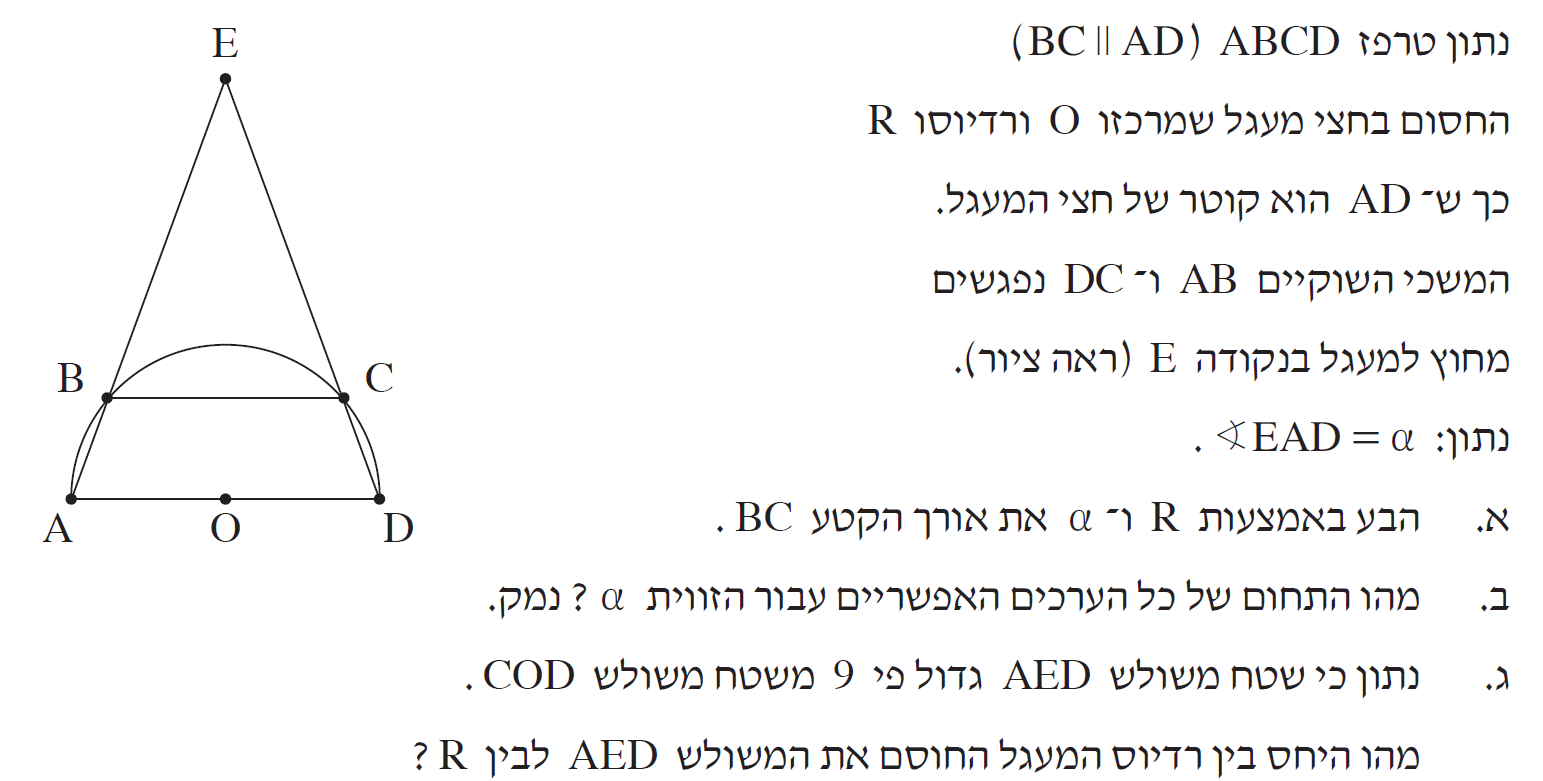
\includegraphics[width=\textwidth]{winter-2017-5}
\end{center}

\textbf{סעיף א}

להלן ההצדקה לסימונים של הזוויות בתרשים להלן. הרדיוסים של המעגל שווים
$OA=OB=OC=OD=R$,
לכן
$\triangle ABO$
שווה-שוקיים, ו-%
$\angle BAO=\angle ABO=\alpha$.
כדי להשלים זוויות של
$\triangle ABO$
ל-%
$180$,
$\angle AOB=180-2\alpha$
שנסמן
$\beta$.
$\angle BCO=\angle AOB=\beta$
לפי זוויות מתחלפות, ו-%
$\angle BCO=\angle CBO=\beta$
כי
$\triangle BOC$
שווה שוקיים. נשלים את הזוויות של
$\triangle BOC$
ונקבל
$\angle BOC=180-2\beta$
שנסמן 
$\gamma$.
לפי זוויות מתחלפות
$\angle COD=\angle BCO=\beta$.
$\triangle COD$
שווה שוקיים, ולכן
$\angle CDO=\angle OCD=(180-\beta)/2=\alpha$.

אפשר גם להשתמש במשפט
$56$
"ניתן לחסום מרובע במעגל אם ורק אם סכום זוג זוויות נגדיות שווה ל-%
$180^\circ$.
לאחר שהסקנו ש-%
$\angle OAB=\angle ABO=\alpha$
ו-%
$\angle AOB=\angle CBO=180-2\alpha=\beta$,
אפשר לחשב ש-%
$\angle CDO=\alpha$
ומשם את שאר הזוויות.
\vspace{-1ex}

\begin{center}
\selectlanguage{english}
\begin{tikzpicture}%[scale=1.1]
\coordinate (A) at (0,0);
\draw[thick] (A) -- ++(6,0) coordinate (D) -- ++(120:3) coordinate (C);
\draw[thick] (A) -- ++(60:3) coordinate (B) -- node[above] {$a$} (C);
\coordinate (O) at (3,0);
\draw[thick] (D) arc(0:180:3);
\path[name path=ae] (A) -- ($(A) ! 2.1 ! (B)$);
\path[name path=de] (D) -- ($(D) ! 2.1 ! (C)$);
\path[name intersections={of=ae and de,by={E}}];
\draw[thick] (B) -- (E) -- (C);
\fill (A) node[below left] {$A$} node[above right,xshift=4pt] {$\alpha$} circle(1.5pt);
\fill (B) node[above left] {$B$} node[below,yshift=-6pt] {$\alpha$} node[below right,xshift=8pt] {$\beta$} circle(1.5pt);
\fill (C) node[above right] {$C$} node[below,yshift=-6pt] {$\alpha$} node[below left,xshift=-8pt] {$\beta$} circle(1.5pt);
\fill (D) node[below right] {$D$}  node[above left,xshift=-4pt] {$\alpha$} circle(1.5pt);
\fill (E) node[above] {$E$} circle(1.5pt);
\fill (O) node[below] {$O$} node[above left,xshift=-8pt] {$\beta$} node[above right,xshift=8pt] {$\beta$} node[above,yshift=4pt] {$\gamma$} circle(1.5pt);
\path (O) -- node[below] {$R$} (A);
\path (O) -- node[below] {$R$} (D);
\draw[thick,dashed] (O) -- node[left,xshift=-2pt] {$R$} (B);
\draw[thick,dashed] (O) -- node[right] {$R$} (C);
\end{tikzpicture}
\end{center}

\np

נחשב
$a=BC$
לפי חוק הסינוסים ולפי חוק הקוסינוסים c-%
$\triangle BOC$,
ותחליטו איזו שיטה עדיפה.

לפי חוק הסינוסים:

\vspace{-5ex}

\erh{12pt}
\begin{equationarray*}{rcl}
\frac{a}{\sin\gamma} &=& \frac{R}{\sin\beta}\\
a &=& \frac{R\sin(180-2\beta)}{\sin\beta} =\frac{R\sin 2\beta}{\sin\beta}\\
&=&\frac{R(2\sin \beta\cos\beta)}{\sin\beta}\\
&=&2R\cos\beta = 2R\cos(180-2\alpha)\\
&=&-2R\cos 2\alpha\,.
\end{equationarray*}

\vspace{-5ex}

לפי חוק הקוסינוסים:
\erh{4pt}
\begin{equationarray*}{rcl}
a^2 &=& R^2+R^2-2R\cdot R \cos \gamma\\
&=&2R^2(1-\cos(180-2\beta)) =2R^2(1+\cos 2\beta)\\
&=&2R^2(1+\cos^2\beta-\sin^2\beta)\\
&=&2R^2(2\cos^2\beta)\\
a&=&2R\cos \beta= 2R\cos(180-2\alpha)\\
&=&-2R\cos 2\alpha\,.
\end{equationarray*}

\vspace{-6ex}

\textbf{סעיף ב}

האורך של צלע חייב להיות חיובי
$a\!=\!-2R\cos 2\alpha\!>\!0$,
ולכן
$\cos 2\alpha\!<\!0$
ו-%
$2\alpha$
נמצא ברביע השני:
\begin{eqnarray*}
90<2\alpha\leq 180\\
45<\alpha\leq 90\,.
\end{eqnarray*}

\vspace{-5ex}

$\alpha \neq 90$
כי הזוויות הבסיס של משולש שווה-שוקיים חייבים להיות פחות מ-%
$90$.



\textbf{סעיף ג}


נתון יחס של השטחים של שני משולשים. נחשב את השטחים של שני המשולשים ונראה מה יוצא.

נחשב 
$S_{\triangle AED}$
לפי הנוסחה הגיאומטרית. הגובה של 
$\triangle AED$
הוא
$h=R\tan\alpha$,
ו:
\[
S_{\triangle AED}= \frac{1}{2}\cdot 2R \cdot h =R^2\tan\alpha\,.
\]

\vspace{-3ex}

נחשב 
$S_{\triangle COD}$
לפי הנוסחה הטריגונומטרית:
\erh{12pt}
\begin{equationarray*}{rcl}
S_{\triangle COD}&=&\frac{1}{2}R\cdot R \cdot \sin \beta\\
&=&\frac{1}{2}R^2 \sin (180-2\alpha)=\frac{1}{2}R^2 \sin 2\alpha\,.
\end{equationarray*}

\np

\begin{center}
\selectlanguage{english}
\begin{tikzpicture}%[scale=1.1]
\clip (-1,-.5) rectangle +(8,6.2);
\coordinate (A) at (0,0);
\draw[thick] (A) -- ++(6,0) coordinate (D) -- ++(120:3) coordinate (C);
\draw[thick] (A) -- ++(60:3) coordinate (B) -- (C);
\coordinate (O) at (3,0);
\path[name path=ae] (A) -- ($(A) ! 2.1 ! (B)$);
\path[name path=de] (D) -- ($(D) ! 2.1 ! (C)$);
\path[name intersections={of=ae and de,by={E}}];
\draw[thick] (B) -- (E) -- (C);
\fill (A) node[below left] {$A$} node[above right,xshift=4pt] {$\alpha$} circle(1.5pt);
\fill (B) node[above left] {$B$} circle(1.5pt);
\fill (C) node[above right] {$C$} circle(1.5pt);
\fill (D) node[below right] {$D$}  node[above left,xshift=-4pt] {$\alpha$} circle(1.5pt);
\fill (E) node[above] {$E$} circle(1.5pt);
\fill (O) node[below] {$O$} node[above right,xshift=8pt] {$\beta$} circle(1.5pt);
\path (O) -- node[below] {$R$} (D);
\path (O) -- node[left] {$R$} (C);
\path (O) -- node[below] {$R$} (A);
\draw[ultra thick] (A) -- (E) -- (D) -- cycle;
\draw[ultra thick] (C) -- (O);
\draw[thick,dashed] (E) -- node[left,near start] {$h$} (O);
\draw[thick] (O) -- (B);
\tkzCircumCenter(A,E,D)\tkzGetPoint{M}
\tkzDrawCircle[thick,dotted,name path=circle](M,A)
\end{tikzpicture}
\end{center}

לפי היחס נתון בין השטחים:
\erh{12pt}
\begin{equationarray*}{rcl}
tR^2\tan\alpha &=& 9\cdot \frac{1}{2}R^2\sin 2\alpha\\
\frac{\sin\alpha}{\cos\alpha} &=& 9\cdot \frac{1}{2} \cdot 2\sin\alpha\cos\alpha\\
\cos\alpha &=& \frac{1}{3}\\
\sin\alpha &=& \sqrt{1-\frac{1}{9}} = \sqrt{\frac{8}{9}}=\frac{2\sqrt{2}}{3}\,.
\end{equationarray*}

\vspace{-3ex}

במשולש 
$\triangle DOE$
יש לנו
$R=DE\cos\alpha$.
נשתמש בחוק הסינוסים כדי לחשב 
$r$,
הרדיוס של המגעל שחוסם 
$\triangle AED$:
\erh{14pt}
\begin{equationarray*}{rcl}
2r&=&\frac{DE}{\sin \alpha}\\
\frac{r}{R}&=&\frac{1}{2\sin \alpha\cos\alpha}\\
&=&\frac{1}{2(2\sqrt{2}/3)(1/3)}\\
&=&\frac{9}{4\sqrt{2}}=1.591\,.
\end{equationarray*}

%%%%%%%%%%%%%%%%%%%%%%%%%%%%%%%%%%%%%%%%%%%%%%%%%%%%%%%%%%%%%%

\np

\section{קיץ תשע"ו מועד ב}

\begin{center}
\selectlanguage{english}
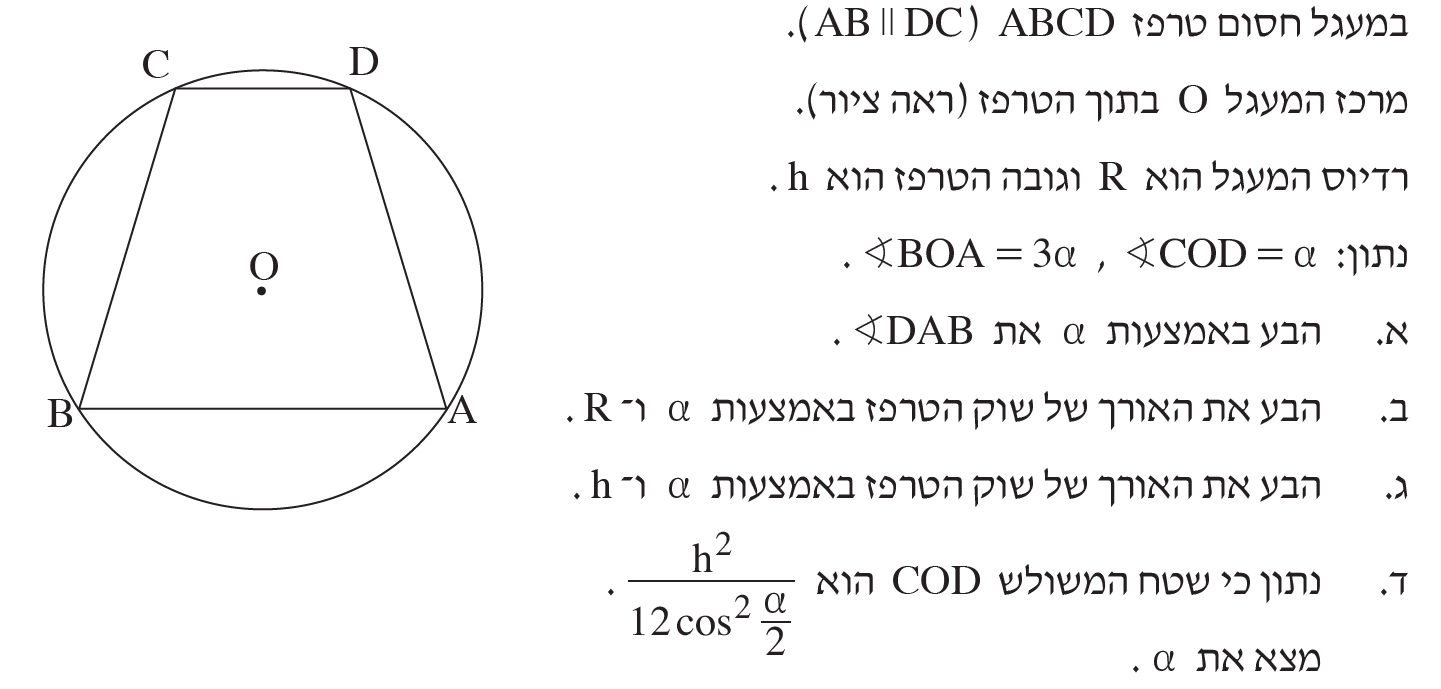
\includegraphics[width=\textwidth]{summer-2016b-5}
\end{center}

\vspace{-2ex}


מהתרשים נראה שהטרפז שווה-שוקיים, אבל אין לסמוך על תרשימים. השקעתי זמן רב עד שעלה בדעתי האפשרות שטרפז חסום במעגל חייב להיות שווה-שוקיים. המשפט לא מופיע ברשימת המשפטים שניתן לצטט בבחינת הבגרות ויש להוכיח אותו. בספרי לימוד המשפט לא מובלט ומופיע רק כדוגמה או תרגיל. אני אביא שתי הוכחות: אחת שלי ואחת המופיעה בספרים.

ההוכחה מהספרים )רשים ימני למטה(:
$\angle ACD = \angle CAB$
לפי זוויות מתחלפות ולכן גם המיתרים הכלואים שווים
$CB=AD$.

ההוכחה שלי )תרשים שמאלי למטה(: המשפט הראשון שחשבתי עליו כאשר קראתי את השאלה הוא משפט 
$56$
"ניתן לחסום מרובע במעגל אם ורק אם סכום זוג זוויות נגדיות שווה ל-%
$180^\circ$".
נסמן
$\angle DAB=\theta$,
ולפי המשפט 
$\angle DCB=180\!-\!\theta$.
לפי זוויות משלימות ומתאימות
$\angle DCF=\angle ABC=\theta$.
לפי משפט
$40$
"טרפז בו הזוויות שליד אותו בסיס שוות זו לזו הוא טרפז שווה שוקיים", הטרפז שווה-שוקיים.

\vspace{-4ex}

\begin{center}
\selectlanguage{english}
\begin{tikzpicture}[scale=.7]
\coordinate (O) at (2,1.5);
\coordinate (B) at (0,.2);
\coordinate (A) at (4,.2);
\node[draw,thick,circle through=(A),name path=circle] at (O) {};
\fill (B) node[left,xshift=-2pt] {$B$} node[above right] {$\theta$?}  circle(1.5pt);
\fill (A) node[right] {$A$} circle(1.5pt);
\path[name path=bc] (B) -- +(75:4);
\path[name path=ad] (A) -- +(105:4);
\path[name intersections={of=bc and circle,by={C}}];
\path[name intersections={of=ad and circle,by={D}}];
\fill (C) node[above left] {$C$} circle(1.5pt);
\fill (D) node[above right] {$D$} circle(1.5pt);
\draw[thick] (B) -- (A) node[above left,xshift=-2pt] {$\theta$} -- (D) -- (C) node[below right,xshift=-2pt] {$180\!-\!\theta$} node[above right,xshift=2pt,yshift=2pt] {$\theta$} -- cycle;
\draw[thick] (B) -- ($(B)!1.3!(C)$) coordinate (F);
\fill (F) node[above right] {$F$} circle(1.5pt);
\end{tikzpicture}
\hspace{4em}
\begin{tikzpicture}[scale=.7]
\coordinate (O) at (2,1.5);
\coordinate (B) at (0,.2);
\coordinate (A) at (4,.2);
\node[draw,thick,circle through=(A),name path=circle] at (O) {};
\fill (B) node[left,xshift=-2pt] {$B$}  circle(1.5pt);
\fill (A) node[right] {$A$} circle(1.5pt);
\path[name path=bc] (B) -- +(75:4);
\path[name path=ad] (A) -- +(105:4);
\path[name intersections={of=bc and circle,by={C}}];
\path[name intersections={of=ad and circle,by={D}}];
\fill (C) node[above left] {$C$} circle(1.5pt);
\fill (D) node[above right] {$D$} circle(1.5pt);
\draw[thick] (B) -- (A) --(D) -- (C) -- cycle;
\draw[thick] (C) node[below right,xshift=10pt] {$\theta$} -- (A) node[above left,xshift=-10pt] {$\theta$};
\end{tikzpicture}
\end{center}

\textbf{סעיף א}

בארבעת המשולשים עם קודקוד
$O$,
הצלעות המקווקוות הם רדיוסים שאורכם
$R$,
והמשולשים שווה שוקיים.
$\triangle COB\cong \triangle DOA$
לפי צ.צ.צ. כי הטרפז שווה שוקיים. מכאן ש-%
$\angle COB\cong \angle DOA$,
וניתן לסמן את הזוויות לפי החישובים מימין לתרשים. החישוב של
$\gamma$
מוצדק כי סכום הזוויות סביב נקודה הוא 
$360$.
השורה האחרונה מציגה את התשובה לשאלה כי
$\angle DAB=\beta+\delta$.

\np

\selectlanguage{english}
\hspace{2em}
\begin{minipage}{.38\textwidth}
\begin{tikzpicture}%[scale=.95]
\coordinate (O) at (2,1.5);
\coordinate (B) at (0,.2);
\coordinate (A) at (4,.2);
\node[draw,thick,circle through=(A),name path=circle] at (O) {};
\fill (O) node[left,xshift=-4pt,yshift=2pt] {$O$} node[below,yshift=-6pt] {$3\alpha$} node[above,yshift=10pt] {$\alpha$} node[right,xshift=6pt] {$\gamma$} circle(1.5pt);
\fill (B) node[left,xshift=-2pt] {$B$} node[above right,xshift=26pt] {$\beta$} circle(1.5pt);
\fill (A) node[right] {$A$} node[above left,xshift=-22pt] {$\beta$} node[above left,xshift=-6pt,yshift=14pt] {$\delta$} circle(1.5pt);
\path[name path=bc] (B) -- +(75:4);
\path[name path=ad] (A) -- +(105:4);
\path[name intersections={of=bc and circle,by={C}}];
\path[name intersections={of=ad and circle,by={D}}];
\fill (C) node[above left] {$C$} circle(1.5pt);
\fill (D) node[above right] {$D$} node[below left,xshift=4pt,yshift=-12pt] {$\delta$}  circle(1.5pt);
\draw[thick] (B) -- (A) --(D) -- (C) -- cycle;
\draw[thick,dashed] (O) -- (A);
\draw[thick,dashed] (O) -- (B);
\draw[thick,dashed] (O) -- (C);
\draw[thick,dashed] (O) -- (D);
\draw[very thick,dotted] (C) -- node[right,yshift=4pt] {$h$} ($(B)!(C)!(A)$) node[below] {$E$};
\draw[rotate=90] ($(B)!(C)!(A)$) rectangle +(6pt,6pt);
\end{tikzpicture}
\end{minipage}
\begin{minipage}{.47\textwidth}
\erh{12pt}
\begin{equationarray*}{rcl}
\beta &\!\!=\!\!& \frac{180\!-\!3\alpha}{2}\\
\gamma &\!\!=\!\!& \frac{360\!-\!(\alpha\!+\!3\alpha)}{2}=180\!-\!2\alpha\\
\delta &\!\!=\!\!&\frac{180\!-\!\gamma}{2}= \frac{180\!-\!(180\!-\!2\alpha)}{2}=\alpha\\
\beta\!+\!\delta&\!\!=\!\!&\frac{180\!-\!\alpha}{2}\,.
\end{equationarray*}
\end{minipage}
\selectlanguage{hebrew}

\textbf{סעיף ב}

כדי חשב אורך של שוק נחפש משולש שאחד מצלעותיו הוא
$DA$.
לפי חוק בסינוסים ב-%
$\triangle DOA$:
\erh{12pt}
\begin{equationarray*}{rcl}
\frac{DA}{\sin\gamma}&=&\frac{R}{\sin\delta}\\
\frac{DA}{\sin(180\!-\!2\alpha)}&=&\frac{R}{\sin\alpha}\\
DA&=&\frac{R\sin 2\alpha}{\sin\alpha}\\
&=&\frac{R\cdot 2\sin \alpha\cos\alpha}{\sin\alpha} = 2R\cos\alpha\,.
\end{equationarray*}

\vspace{-4ex}

\textbf{סעיף ג}

בתרשים ציירנו את הגובה מהנקודה 
$C$
כדי לא להסתיר את הסימונים ב-%
$\triangle DOA$.
$CB=DA$
הוא גם שוק. נשתמש בהגדרה של סינוס במשולש 
$\triangle CBE$:
\[
\frac{h}{CB}=\sin \angle CBE=\sin \left(\frac{180\!-\!3\alpha}{2}+\alpha\right)=\sin \left(90-\frac{\alpha}{2}\right)=\cos\frac{\alpha}{2}\,.
\]
כי
$\angle CBE=\angle DAB=\beta+\delta$.
התשובה היא
$CB=\displaystyle\frac{h}{\cos (\alpha/2)}$.

\textbf{סעיף ד}

בנוסחה הטריגונטמרית עבור
$S_{\triangle COD}$
יופיעו אורכי הצלעות
$R$
והזווית
$\alpha$.
אנו רוצים נוסחה עם 
$h$
ו-%
$\alpha$
כדי להשוות לביטוי הנתון. נשווה את הביטויים עבור שוקי הטרפז מהסעיפים הקודמים:
\erh{12pt}
\begin{equationarray*}{rcl}
2R\cos\alpha&=&\frac{h}{\cos(\alpha/2)}\\
R&=&\frac{h}{2\cos\alpha \cos(\alpha/2)}\,.
\end{equationarray*}

\np

נציב בנוסחה לשטח, נשווה לנוסחה הנתונה לשטח ונצמצם:
\erh{16pt}
\begin{equationarray*}{rcl}
S_{\triangle COD}&=&\frac{1}{2}\cdot OC \cdot OD \cdot \sin\alpha=\frac{1}{2}R^2\sin\alpha\\
&=&\frac{1}{2}\cdot \frac{h^2}{4}\cdot \frac{1}{\left(\cos\alpha \cos(\alpha/2)\right)^2} \cdot \sin\alpha\\
\frac{h^2}{12\cos^2 (\alpha/2)}&=&\frac{1}{2}\cdot \frac{h^2}{4}\cdot \frac{1}{\left(\cos\alpha \cos(\alpha/2)\right)^2} \cdot \sin\alpha\\
\frac{1}{12}&=&\frac{1}{8}\cdot \frac{1}{\cos^2\alpha} \cdot \sin\alpha\\
\frac{1}{12}&=&\frac{1}{8}\cdot \frac{1}{1-\sin^2\alpha} \cdot \sin\alpha\,.
\end{equationarray*}
נקבל משוואה ריבועית ב-%
$\sin\alpha$,
ונבחר את השורש 
$\displaystyle\frac{1}{2}$
כי הערך של סינוס לא יכול להיות
$-2$:
\erh{12pt}
\begin{equationarray*}{rcl}
2\sin^2\alpha + 3\sin\alpha - 2&=&0\\
(2\sin\alpha-1)(\sin\alpha+2)&=& 0\\
\sin\alpha&=&\frac{1}{2}\,.
\end{equationarray*}
הערך היחיד ש-%
$\alpha$
יכול לקבל הוא
$30^\circ$
כי זוויות הבסיס של טרפז חייבים להיות פחות מ-%
$90^\circ$.

%%%%%%%%%%%%%%%%%%%%%%%%%%%%%%%%%%%%%%%%%%%%%%%%%%%%%%%%%%%%%%


\np

\section{קיץ תשע"ו מועד א}

\begin{center}
\selectlanguage{english}
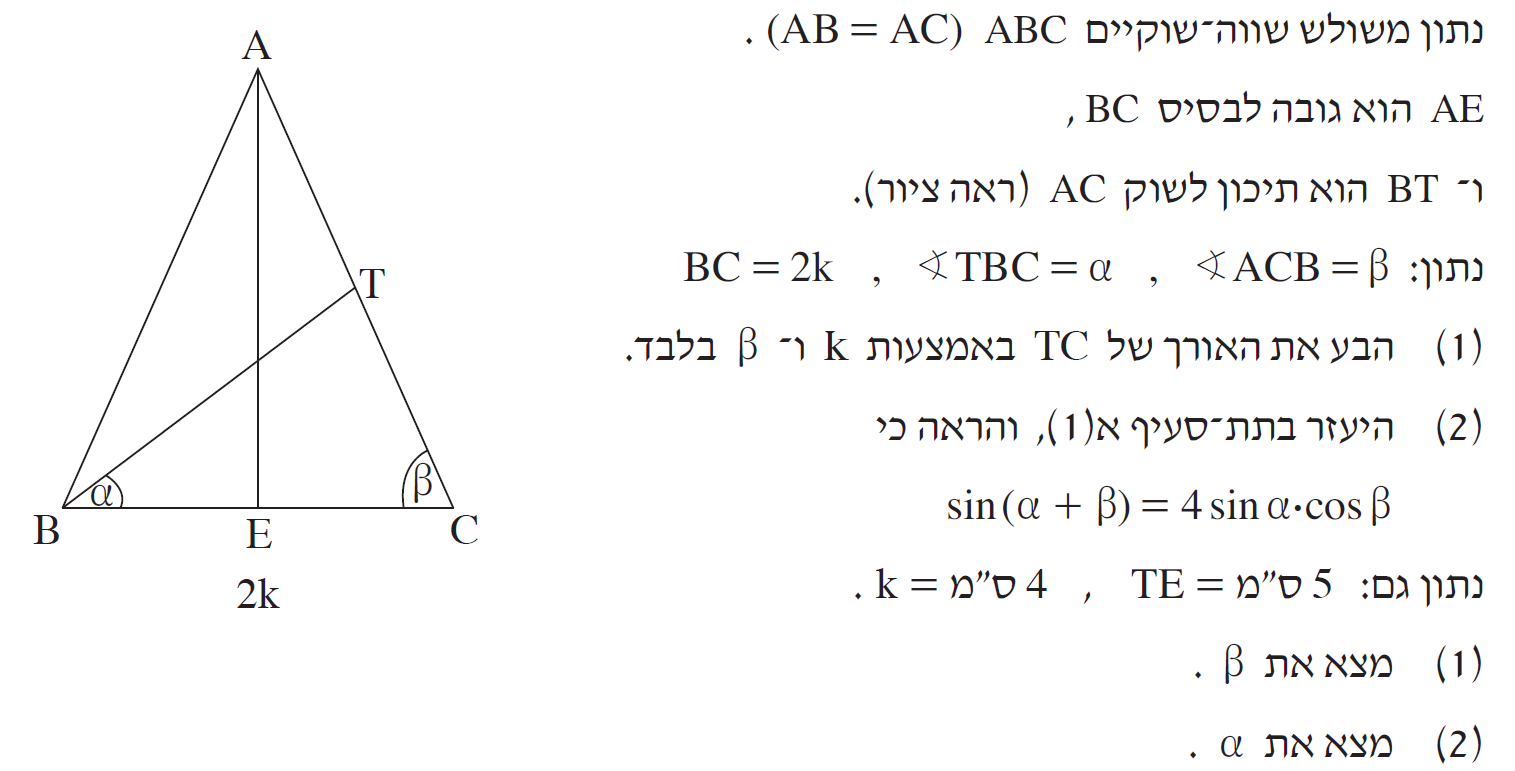
\includegraphics[width=\textwidth]{summer-2016a-5}
\end{center}

\vspace{-3ex}

\begin{center}
\selectlanguage{english}
\begin{tikzpicture}[scale=.85]
\coordinate (B) at (0,0);
\coordinate (C) at (5,0);
\path[name path=ba] (B) -- +(66:7);
\path[name path=ca] (C) -- +(114:7);
\path[name intersections={of=ba and ca,by={A}}];
\fill (A) node[above] {$A$} circle(1.5pt);
\fill (B) node[below left] {$B$} node[above right,xshift=12pt] {$\alpha$} circle(1.5pt);
\fill (C) node[below right] {$C$} node[above left,xshift=-6pt] {$\beta$} circle(1.5pt);
\coordinate (T) at ($(A)!.5!(C)$);
\fill (T) node[right] {$T$} circle(1.5pt);
\draw[thick] (B) -- (T);
\coordinate (E) at ($(B)!(A)!(C)$);
\draw[thick] (A) -- (E);
\fill (E) node[below] {$E$} circle(1.5pt);
\draw[rotate=90] (E) rectangle +(8pt,8pt);
\draw[thick] (A) -- node[left] {$2a$} (B) -- node[below] {$k$} (E) -- node[below] {$k$} (C) -- node[right] {$a$} (T) -- node[right] {$a$} (A);
\node at ($(T)+(60pt,-10pt)$) {$180\!-\!(\alpha\!+\!\beta)$};
\draw[->] ($(T)+(25pt,-9pt)$) -- +(-28pt,0);
\end{tikzpicture}
\end{center}

\vspace{-1ex}

$\bm{(1)}$
לפי הגדרת קוסינוסים ב-%
$\triangle AEC$:

\vspace{-3ex}

\erh{12pt}
\begin{equationarray*}{rcl}
\cos \beta &=& \frac{k}{2a}\\
TC = a &=& \frac{k}{2\cos\beta}\,.
\end{equationarray*}

\vspace{-2ex}

$\bm{(2)}$
נחפש משולש עבורו חוק הסינוסים ייתן משוואה בה יצטמצם
$k$
או
$a$.
$\triangle TBC$ 
מתאים:

\vspace{-5ex}

\selectlanguage{english}
\erh{14pt}
\begin{equationarray*}{rcl}
\frac{2k}{\sin(180\!-\!(\alpha\!+\!\beta))}&=&\frac{a}{\sin\alpha}\\
\frac{2k}{\sin(\alpha\!+\!\beta)}&=&\frac{k/(2\cos\beta)}{\sin\alpha}\\
\sin(\alpha\!+\!\beta)&=&4\sin\alpha\cos\beta\,.
\end{equationarray*}
\selectlanguage{hebrew}

\np

$\bm{(1)}$
נוסיף את אורכי הצלעות הנתונים ונשתמש במשפט
$86$
"במשולש ישר זווית התיכון ליתר שווה למחצית היתר" כדי להסיק ש-%
$TE=TA=TC=5$
ו-%
$\triangle ETC$
שווה-שוקיים:
\begin{center}
\selectlanguage{english}
\begin{tikzpicture}[scale=.9]
\coordinate (B) at (0,0);
\coordinate (C) at (5,0);
\path[name path=ba] (B) -- +(66:7);
\path[name path=ca] (C) -- +(114:7);
\path[name intersections={of=ba and ca,by={A}}];
\fill (A) node[above] {$A$} circle(1.5pt);
\fill (B) node[below left] {$B$} node[above right,xshift=12pt] {$\alpha$} circle(1.5pt);
\fill (C) node[below right] {$C$} node[above left,xshift=-6pt] {$\beta$} circle(1.5pt);
\coordinate (T) at ($(A)!.5!(C)$);
\fill (T) node[right] {$T$} circle(1.5pt);
\draw[thick] (B) -- (T);
\coordinate (E) at ($(B)!(A)!(C)$);
\draw[thick] (A) -- (E);
\fill (E) node[below] {$E$} node[above right,xshift=2pt] {$\beta$}circle(1.5pt);
\draw[rotate=90] (E) rectangle +(8pt,8pt);
\draw[thick] (A) -- (B) -- (C) -- node[right] {$5$} (T) -- node[right] {$5$} (A);
\coordinate (F) at ($(E)!(T)!(C)$);
\draw[thick,dashed] (E) -- node[above,xshift=-2pt] {$5$} (T) -- (F);
\path (B) -- node[below] {$4$} (E) -- node[below] {$2$} (F) -- node[below] {$2$} (C);
\draw (F) rectangle +(8pt,8pt);
\end{tikzpicture}
\end{center}

נוריד גובה מ-%
$T$
שהוא אנך אמצעי במשלוש שווה-שוקיים
$\triangle ETC$
ונקבל:
\erh{10pt}
\begin{equationarray*}{rcl}
\cos\beta &=& \frac{2}{5}\\
\beta &=&66.4^\circ\,.
\end{equationarray*}

\vspace{-4ex}

$\bm{(2)}$
לפי סעיף 
$(1)$
וסעיף 
$(2)$
הקודם:

\vspace{-5ex}

\erh{14pt}
\begin{equationarray*}{rcl}
\sin(\alpha+\beta)&=&4\sin\alpha\cos\beta\\
\sin\alpha\cos\beta+\cos\alpha\sin\beta&=&4\sin\alpha\cos\beta\\
\sin\alpha\cdot\frac{2}{5}+\cos\alpha\sqrt{1-\left(\frac{2}{5}\right)^2}&=&4\sin\alpha\cdot\frac{2}{5}\\
\sqrt{21}\cos\alpha&=&6\sin\alpha\\
\tan\alpha &=& \frac{\sqrt{21}}{6}\\
\alpha&=&37.37^\circ\,.
\end{equationarray*}

%%%%%%%%%%%%%%%%%%%%%%%%%%%%%%%%%%%%%%%%%%%%%%%%%%%%%%%%%%%%%%
\np


\section{חורף תשע"ו}

\begin{center}
\selectlanguage{english}
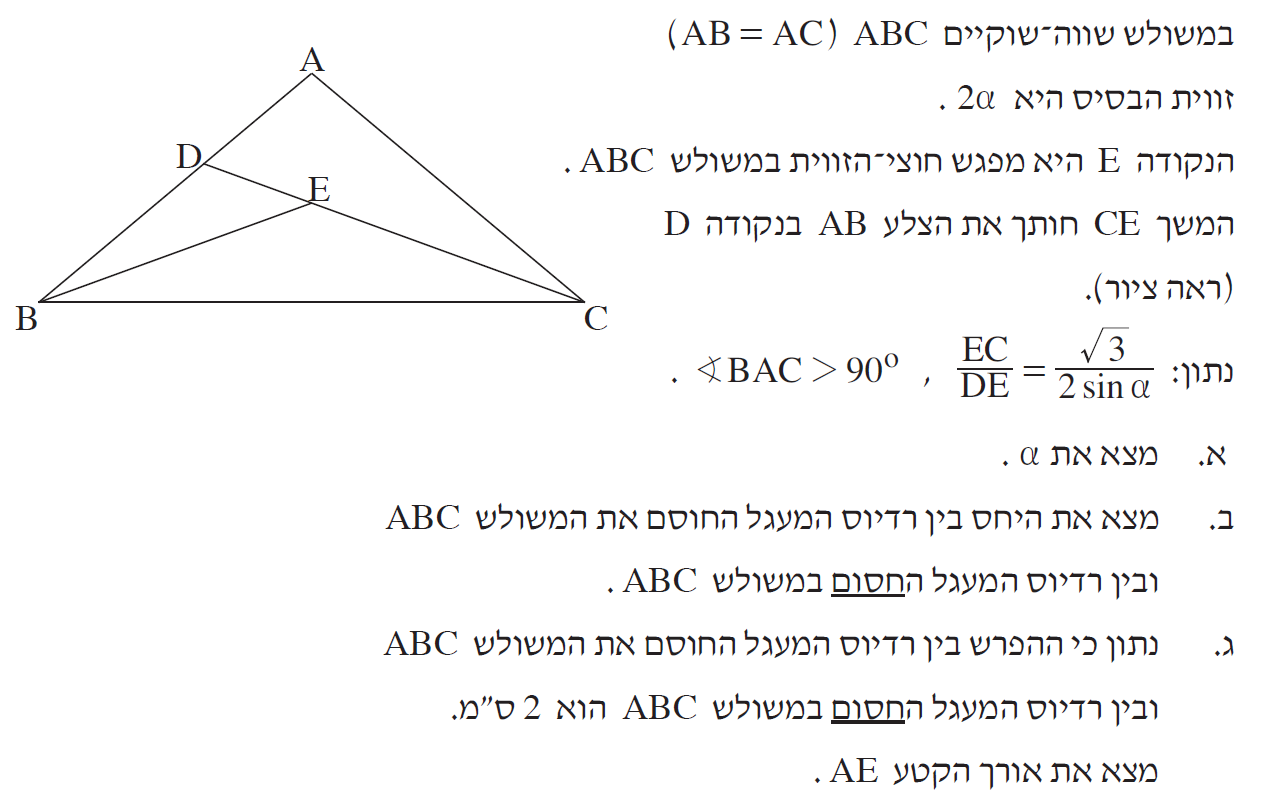
\includegraphics[width=\textwidth]{winter-2016-5}
\end{center}

נתון שהנקודה 
$E$
היא מפגש חוצי הזוויות. לפי משפט
$6$
"במשולש שווה שוקיים , חוצה זווית הראש, התיכון לבסיס והגובה לבסיס מתלכדים", ולכן חוצה הזווית
$\angle BAC$
עובר דרך
$E$
וחותך את
$BC$
בנקודה 
$F$
בזווית ישרה. לפני שניגש לשאלות, נסמן זוויות תוך שימוש רק במשפטים פשוטים כגון סכום הזוויות במשולש הוא
$180$.


\begin{center}
\selectlanguage{english}
\begin{tikzpicture}%[scale=1.1]
\coordinate (B) at (0,0);
\coordinate (C) at (10,0);
\path[name path=ba] (B) -- +(40:7);
\path[name path=ca] (C) -- +(140:7);
\path[name intersections={of=ba and ca,by={A}}];
\fill (A) node[above] {$A$} node[below right,xshift=0pt,yshift=-8pt] {$\gamma$} node[below left,yshift=-8pt] {$\gamma$} circle(1.5pt);
\fill (B) node[below left] {$B$} node[above right,xshift=24pt,yshift=12pt] {$\alpha$} node[above right,xshift=30pt] {$\alpha$} circle(1.5pt);
\fill (C) node[below right] {$C$} node[above left,xshift=-24pt,yshift=12pt] {$\alpha$} node[above left,xshift=-30pt] {$\alpha$} circle(1.5pt);
\draw[thick] (A) -- (B) -- (C) -- cycle;
\path[name path=cbis] (C) -- +(160:8);
\path[name path=bbis] (B) -- +(20:8);
\path[name intersections={of=ba and cbis,by={D}}];
\path[name intersections={of=bbis and cbis,by={E}}];
\fill (D) node[left] {$D$} node[right,xshift=8pt,yshift=2pt] {$3\alpha$} node[below left,xshift=-20pt] {$180\!-\!3\alpha$} circle(1.5pt);
\draw[->] ($(D)+(-22pt,-10pt)$) -- +(20pt,0);
\fill (E) node[above right] {$E$} node[above left,yshift=2pt] {$\beta$} node[below left,yshift=-4pt] {$\beta$} node[below right,yshift=-4pt] {$\beta$} node[left,xshift=-10pt] {$2\alpha$} circle(1.5pt);
\draw[thick] (C) -- (D);
\draw[thick] (B) -- node[above] {$a$} (E);
\path (C) -- node[above] {$a$} (E);
\coordinate (F) at (A |- B);
\draw[thick,dashed] (A) -- (F);
\fill (F) node[below] {$F$} circle(1.5pt);
\draw (F) rectangle +(8pt,8pt);
\node at ($(A)+(80pt,-10pt)$) {$\beta = 90\!-\!\alpha$};
\node at ($(A)+(83pt,-26pt)$) {$\gamma = 90\!-\!2\alpha$};
\path (E) -- node[right,yshift=-4pt] {$r$} (F);
\end{tikzpicture}
\end{center}


$\triangle EFB\cong \triangle EFC$
לפי צלע-צלע במשולש ישר-זווית: 
$F$
היא נקודת האמצע של
$BC$
ו-%
$EF$
הוא צלע משותף. לכן
$\angle BEF=\angle CEF=90\!-\!\alpha$
שנסמן 
$\beta$.

בדרך דומה נראה ש-%
$\angle BAF=\angle CAF=90\!-\!2\alpha$
שנסמן
$\gamma$.

$\angle AED=\beta$
לפי זוויות קודקודיות, ו-%
$\angle ADE=180-\beta-\gamma=3\alpha$.

לבסוף, 
$\angle BDE=180\!-\!3\alpha$
לפי זוויות משלימות.

\np

\textbf{סעיף א}

נתון היחס 
$\displaystyle\frac{EC}{DE}$
כתלות ב-%
$\alpha$,
ולכן נחפש משלוש שעבורו חוק הסינוסים ייתן יחס אחר כתלות ב-%
$\alpha$,
ואז תהיה לנו משוואה ב-%
$\alpha$
בלבד. אמנם 
$EC,DE$
הם צלעות במשולשים שונים, אבל כבר הוכחנו ש-%
$\triangle EFB\cong \triangle EFC$
כך ש-%
$EB=EC$.
לפי חוק הסינוסים ב-%
$\triangle BDE$:
\erh{14pt}
\begin{equationarray*}{rcl}
\frac{EB}{\sin(180\!-\!3\alpha)}&=&\frac{DE}{\sin\alpha}\\
\frac{EB}{DE}&=&\frac{\sin(180\!-\!3\alpha)}{\sin\alpha}=\frac{\sin 3\alpha}{\sin\alpha}= \frac{\sqrt{3}}{2\sin\alpha}\\
\sin 3\alpha&=&\frac{\sqrt{3}}{2}\\
\alpha&=&20^\circ\,.
\end{equationarray*}

\vspace{-5ex}

\textbf{סעיף ב}

לפי משפט
$49$
"שלושת חוצי הזוויות של משולש נחתכים בנקודה אחת, שהיא מרכז המעגל החסום במשולש", הנקודה
$E$
היא מרכז המעגל החסום שמשיק לצלע המשולש ב-%
$F$.
$r=EF$
הוא הרדיוס של המעגל החסום.

כעת צריך להיזהר שלא לקבוע ש-%
$E$
היא מרכז המעגל החוסם כי אין אנו יודעים שחוצי הזוויות האחרות הם גם אנכים אמצעיים. במקום זה נשתמש בחוק הסינוסים על המשלוש
$\triangle ABC$.
נבחר את הזווית
$\angle BAC=180\!-\!4\alpha$,
כי אפשר לחשב את אורך הצלע הנגדי
$BC$
כתלות ב-%
$r,\alpha$:

\vspace{-4ex}
\erh{14pt}
\begin{equationarray*}{rcl}
\tan\alpha &=& \frac{r}{BF}=\frac{r}{BC/2}\\ 
2R&=&\frac{BC}{\sin (180\!-\!4\alpha)}=\frac{2r}{\sin 4\alpha\tan\alpha}\\
\frac{R}{r}&=&\frac{1}{\sin 4\alpha\cdot\tan \alpha}=\frac{1}{\sin 80\cdot\tan 20}=2.79\,.
\end{equationarray*}

\vspace{-2ex}

\textbf{סעיף ג}

נתון
$R-r=2$.
נציב 
$R=2.79r$
שחישבנו בסעיף ב, ונקבל
$r=2/(2.79-1)=1.117$.
אין לנו מספיק מידע על המשולשים
$\triangle AED,\triangle AEC$,
ולכן נחשב
$AF=AE+EF=AE+r$:
\erh{14pt}
\begin{equationarray*}{rcl}
\tan 2\alpha&=&\frac{AE+r}{BF}=\frac{AE+r}{r/\tan\alpha}\\
AE&=&\frac{r(\tan 2\alpha - \tan \alpha)}{\tan \alpha}\\
&=&\frac{1.117(\tan 40-\tan 20)}{\tan 20}=1.458\,.
\end{equationarray*}

%%%%%%%%%%%%%%%%%%%%%%%%%%%%%%%%%%%%%%%%%%%%%%%%%%%%%%%%%%%%%%


\np

\section{קיץ תשע"ה מועד ב}

\begin{center}
\selectlanguage{english}
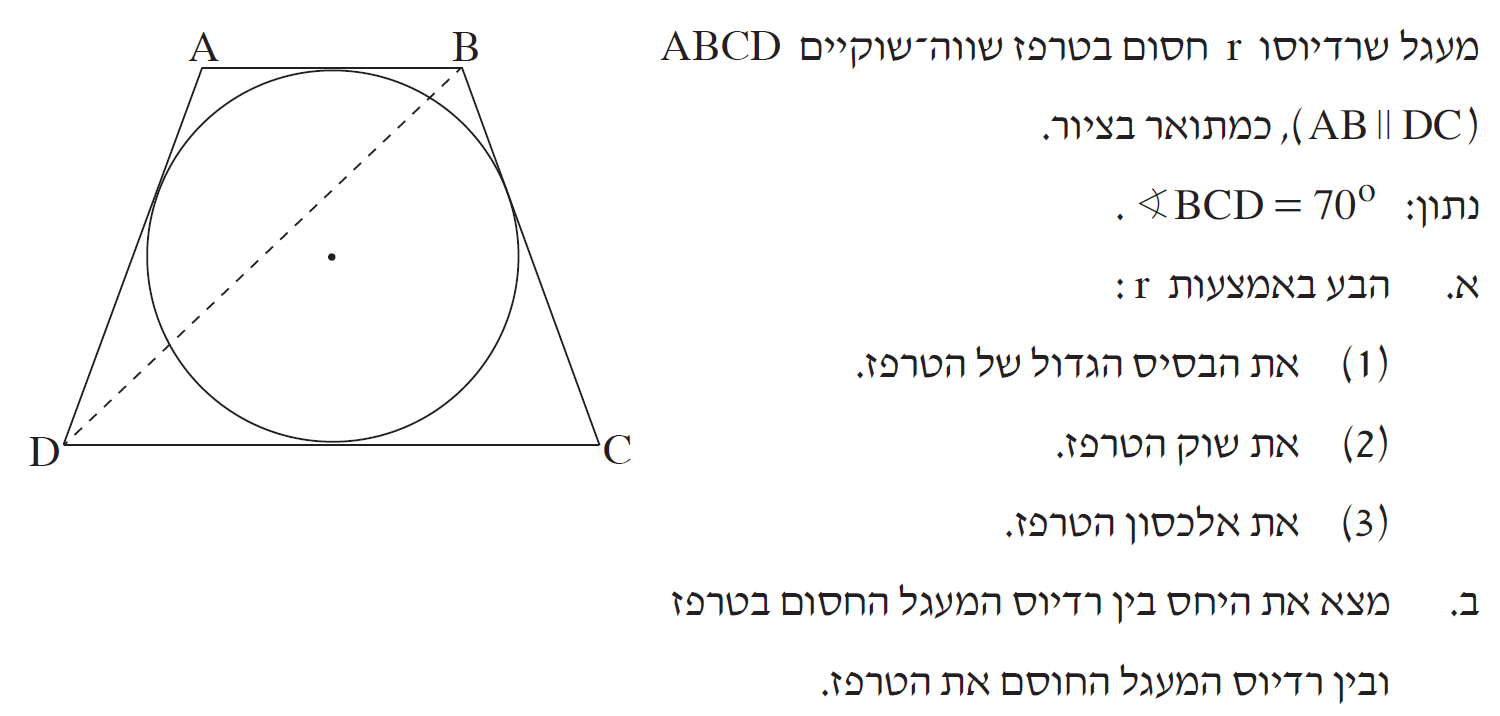
\includegraphics[width=\textwidth]{summer-2015b-5}
\end{center}
נוריד אנך מ-%
$A$
שחתוך את
$DC$
ב-%
$G$,
ואנך מ-%
$B$
שחותך את 
$DC$
ב-%
$H$.
בטרפז
$AB\|DC$
ולכן
$ABHG$
הוא מלבן. לפי משפט
$77$
"המשיק למעגל מאונך לרדיוס בנקודת ההשקה", האנך מנקודת ההשקה של מעגל עם
$AB$
עובר דרך מרכז המעגל והוא ניצב לנקודת ההשקה עם
$DC$.
מכאן ש-%
$AG=EF=BF=2r$.

נסמן
$AB=GH=b_2$.
הטרפז שווה-שוקיים ולפי משפט
$39$
"בטרפז שווה שוקיים הזוויות שליד אותו בסיס שוות זו לזו",
$\angle ADC=\angle BCD=70^\circ$,
$\angle DAG=\angle CBH=20^\circ$.
ביחד עם 
$AD=BC$
בטרפז שווה-שוקיים,
$\triangle ADG \cong \triangle BCH$.
נסמן
$DG=HC=b_1$
ונקבל ש-%
$DC=2b_1+b_2$
שנסמן
$b$.

\begin{center}
\selectlanguage{english}
\begin{tikzpicture}[scale=1]
\node[circle,draw,thick] (In) at (0,0) [minimum size=5cm] {};
\coordinate (D) at (-3.5,-2.5);
\draw[thick] (D) -- +(7,0) coordinate (C) node[above left,xshift=-2pt] {$70$};
\fill (C) node[below right] {$C$} circle(1.5pt);
\fill (D) node[below left] {$D$}  node[above right,xshift=2pt] {$70$} circle(1.5pt);
\coordinate (DA) at (tangent cs:node=In,point={(D)},solution=2);
\path[name path=da] (D) -- ($(D)!1.7!(DA)$);
\fill (DA) circle(1.5pt);
\coordinate (CB) at (tangent cs:node=In,point={(C)},solution=1);
\path[name path=cb] (C) -- ($(C)!1.7!(CB)$);
\fill (CB) circle(1.5pt);
\path[name path=top] (-3,2.5) -- (3,2.5);
\path[name intersections={of=da and top,by={A}}];
\path[name intersections={of=cb and top,by={B}}];
\fill (A) node[above left] {$A$} circle(1.5pt);
\fill (B) node[above right] {$B$} circle(1.5pt);
\draw[thick] (D) -- node[left] {$s$} (A) -- (B) -- node[right] {$s$} (C);
\draw[thick,dashed] (D) -- (B);
\coordinate (AB) at (0,2.5);
\coordinate (DC) at (0,-2.5);
\coordinate (ADC) at ($(D)!(A)!(C)$);
\draw[thick,dashed] (A) -- node[right,yshift=8pt] {$2r$} (ADC);
\fill (ADC) node[below,yshift=-1pt] {$G$} circle(1.5pt);
\coordinate (BDC) at ($(D)!(B)!(C)$);
\draw[thick,dashed] (B) -- node[left,yshift=8pt] {$2r$} (BDC);
\fill (BDC) node[below,yshift=-1pt] {$H$} circle(1.5pt);
\draw (ADC) rectangle +(8pt,8pt);
\draw (BDC) rectangle +(8pt,8pt);
%\draw (DC) rectangle +(8pt,8pt);
\draw[<->] ($(D)+(0,-8mm)$) -- node[fill=white] {$b_1$} ($(ADC)+(0,-8mm)$);
\draw[<->] ($(ADC)+(0,-8mm)$) -- node[fill=white] {$b_2$} ($(BDC)+(0,-8mm)$);
\draw[<->] ($(BDC)+(0,-8mm)$) -- node[fill=white] {$b_1$} ($(C)+(0,-8mm)$);
\draw[<->] ($(D)+(0,-14mm)$) -- node[fill=white] {$b$} ($(C)+(0,-14mm)$);
\draw[<->] ($(A)+(0,8mm)$) -- node[fill=white] {$b_2$} ($(B)+(0,8mm)$);
\end{tikzpicture}
\end{center}

\np

\textbf{סעיף א}

$(1)$
נחפש משפט הקושר צלעות של מרובע עם הרדיוס של המעגל החוסם. משפט
$57$
"מרובע קמור חוסם מעגל אם ורק אם סכום שתי צלעות נגדיות שווה לסכום שתי הצלעות הנגדיות האחרות":
\[
2s=b+b_2=(b_1+b_2+b_1)+b_2=2(b_1+b_2)\,.
\]
ממשוואה זו נחשב משוואת נוספות שיעזרו לנו בהמשך:
\[
s=b_1+b_2,\quad b=2b_1+b_2=s+b_1\,.
\]
לפי ההגדרות של הפונקציות הטריגונומרטיות ב-%
$\triangle ADC$,
נוכל לקשר את 
$r$
לצלעות:
\erh{12pt}
\begin{equationarray*}{rcl}
\tan 70 &=& \frac{2r}{b_1}\\
\sin 70&=&\frac{2r}{s}\\
b&=&s+b_1\\
&=&2r\left(\frac{1}{\sin 70}+\frac{1}{\tan 70}\right)\\
&=&2.856r\,.
\end{equationarray*}

\vspace{-3ex}

$(2)$
$s=\displaystyle\frac{2r}{\sin 70}=2.128r$.

\medskip

$(3)$
האלכסון הוא היתר של 
$\triangle BDH$
שצלעותיו ידועים:

\vspace{-6ex}

\erh{18pt}
\begin{equationarray*}{rcl}
DB^2&=& (b_1+b_2)^2 + (2r)^2=s^2 +(2r)^2\\
&=& \left(\frac{2r}{\sin 70}\right)^2 + 4r^2\\
DB&=&2r\sqrt{\left(\frac{1}{\sin 70}\right)^2+1}=2.921r\,.
\end{equationarray*}

\vspace{-3ex}

\textbf{סעיף ב}

במבט ראשון נראה שכדאי להשתמש במשפט
$56$
"ניתן לחסום מרובע במעגל אם ורק אם סכום זוג זוויות נגדיות שווה ל-%
$180^\circ$",
אבל אין בו צורך. שימו לב שהמרכז של המעגל החוסם לא חופף את המרכז של המעגל החסום, כך שאי-אפשר לחשב 
$R$,
הרדיוס של המעגל החסום, כמרחק ממרכז המעגל החוסם לאחת מקודקודי הטרפז. במקום זה נשתמש בחוק הסינוסים ב-%
$\triangle BCD$:
\erh{16pt}
\begin{equationarray*}{rcl}
2R&=&\frac{DB}{\sin BCD}=\frac{2.921r}{\sin 70}\\
\frac{r}{R}&=&\frac{2\cdot \sin 70}{2.921}=6.434\,.
\end{equationarray*}

%%%%%%%%%%%%%%%%%%%%%%%%%%%%%%%%%%%%%%%%%%%%%%%%%%%%%%%%%%%%%%

\np

\section{קיץ תשע"ה מועד א}

\begin{center}
\selectlanguage{english}
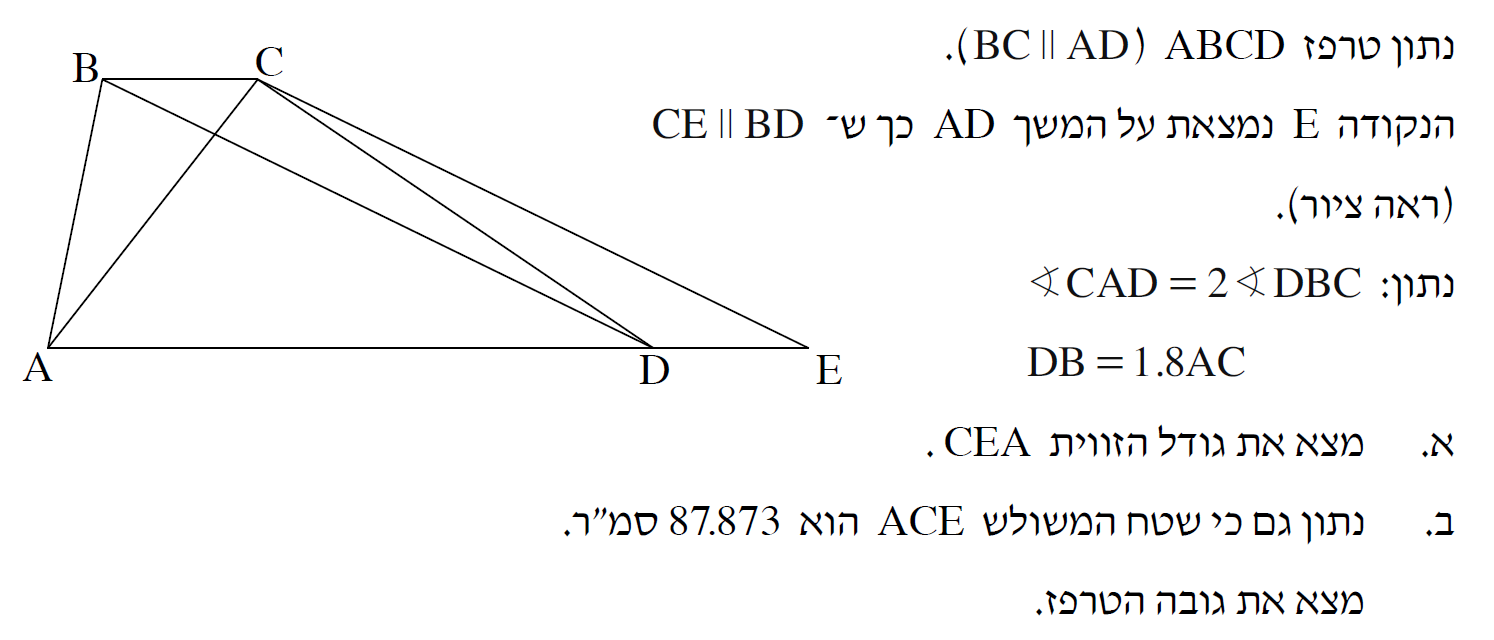
\includegraphics[width=\textwidth]{summer-2015a-5}
\end{center}

\vspace{-1ex}

\textbf{סעיף א}

נסמן זוויות לפי זוויות מתחלפות, מתאימות ופנימיות:
$\angle CBE=\angle BDA=\angle CEA=\alpha$,
$\angle BCE=\angle BDE=180-\alpha$.

\vspace{-2ex}

\begin{center}
\selectlanguage{english}
\begin{tikzpicture}[scale=1.2]
\draw[thick] (0,0) coordinate (A) node[below left] {$A$} -- (6,0) coordinate (D) node[below] {$D$} -- (8,0) coordinate (E) node[below right] {$E$} -- (3,3) coordinate (C) node[above right] {$C$} -- (1,3) coordinate (B) node[above left] {$B$} -- (A) -- node[above,xshift=-2pt] {$a$} (C);
\draw[thick] (B) -- node[below,xshift=-2pt] {$1.8a$} (D) -- (C);
\fill (A) node[above right,xshift=12pt] {$2\alpha$} circle(1.5pt);
\fill (B) node[below right,xshift=16pt] {$\alpha$} circle(1.5pt);
\fill (C) circle(1.5pt);
\fill (D) node[above left,xshift=-16pt] {$\alpha$} circle(1.5pt);
\fill (E) node[above left,xshift=-16pt] {$\alpha$} circle(1.5pt);
\draw[ultra thick] (A) -- (E) -- node[above,xshift=4pt,yshift=2pt] {$1.8a$} (C) -- cycle;
\draw ($(D)+(6mm,0)$) arc[start angle=0,end angle=150,radius=6mm];
\node at ($(E)+(-6pt,30pt)$) {$180\!-\!\alpha$};
\draw[->] ($(E)+(-6pt,25pt)$) -- +(-35pt,-12pt);
\draw ($(C)+(-6mm,0)$) arc[start angle=180,end angle=330,radius=6mm];
\node at ($(C)+(40pt,-4pt)$) {$180\!-\!\alpha$};
\draw[->] ($(C)+(40pt,-8pt)$) -- +(-40pt,-4pt);
\end{tikzpicture}
\end{center}

\vspace{-1ex}

משולש-%
$\triangle CEA$
לאחר שנוכיח ש-%
$CD=DB=1.8a$.
נתון 
$BC\|AD$, $CE\|BD$,
ולפי משפט
$29$
"מרובע שבו כל זוג זוויות נגדיות שוות הוא מקבילית", 
$BCED$
היא מקבילית.

\vspace{-4ex}

\erh{6pt}
\begin{equationarray*}{rcl}
\frac{a}{\sin \alpha} &=& \frac{1.8a}{\sin 2\alpha}=\frac{1.8a}{2\sin \alpha\cos\alpha}\\
\cos \alpha &=& 0.9\\
\alpha &=& 25.84\,.
\end{equationarray*}

\vspace{-4ex}

\textbf{סעיף ב}

נרשום את כל הזוויות ב-%
$\triangle ACE$:
\begin{eqnarray*}
\angle CEA=\alpha &=& 25.84\\
\angle CAE=2\alpha &=& 51.68\\
\angle ACE=180-3\alpha &=& 102.48\,.
\end{eqnarray*}
מהתרשים אפשר לראות ש-%
$S_{\triangle ACE}$
מורכב מסכום השטחים של שני משולשים עם אותו גובה:

\np

\begin{center}
\selectlanguage{english}
\begin{tikzpicture}[scale=1.2]
\draw[thick] (0,0) coordinate (A) node[below left] {$A$} -- (8,0) coordinate (E) node[below right] {$E$} -- (3,3) coordinate (C) node[above right] {$C$} -- (1,3) coordinate (B) node[above left] {$B$} -- (A) -- node[above,xshift=-2pt] {$a$} (C);
\fill (A) node[above right,xshift=12pt] {$2\alpha$} circle(1.5pt);
\fill (B) circle(1.5pt);
\fill (C) circle(1.5pt);
\fill (E) node[above left,xshift=-16pt] {$\alpha$} circle(1.5pt);
\draw[ultra thick] (A) -- (E) -- node[right,xshift=2pt,yshift=2pt] {$1.8a$} (C) -- cycle;
\coordinate (F) at ($(A)!(C)!(E)$);
\draw[thick,dashed] (C) -- node[left] {$h$} (F);
\fill (F) circle(1.5pt);
\draw (F) rectangle +(8pt,8pt);
\path (A) -- node[below] {$b_1$} (F) -- node[below] {$b_2$} (E);
\end{tikzpicture}
\end{center}

\vspace{-6ex}

\erh{12pt}
\begin{equationarray*}{rcl}
S_{\triangle ACE} &=& \frac{1}{2}(b_1+b_2)h\\
b_1&=& \frac{h}{\tan 2\alpha }\\
b_2&=& \frac{h}{\tan \alpha }\\
S_{ACE} &=& \frac{1}{2}h^2\left(\frac{1}{\tan 2\alpha}+\frac{1}{\tan \alpha}\right)\\
87.873 &=& \frac{1}{2}h^2(6.79+2.06) =  1.428 h^2\\
h&=& 7.846\,.
\end{equationarray*}
פתרון אחר משתמש בנוסחה הטריגונומטרית לשטח:
\erh{12pt}
\begin{equationarray*}{rcl}
S_{\triangle ACE} &=& \frac{1}{2}\cdot AC \cdot CE \cdot \sin \angle ACE\\
&=& \frac{1}{2}\cdot a \cdot 1.8a \cdot \sin (180-3\alpha)\\
87.873 &=& 0.87873 a^2\\
a&=&10\\
h &=& a\sin 2\alpha = 7.846\,.
\end{equationarray*}

%%%%%%%%%%%%%%%%%%%%%%%%%%%%%%%%%%%%%%%%%%%%%%%%%%%%%%%%%%%%%%


\np


\section{חורף תשע"ה}

\begin{center}
\selectlanguage{english}
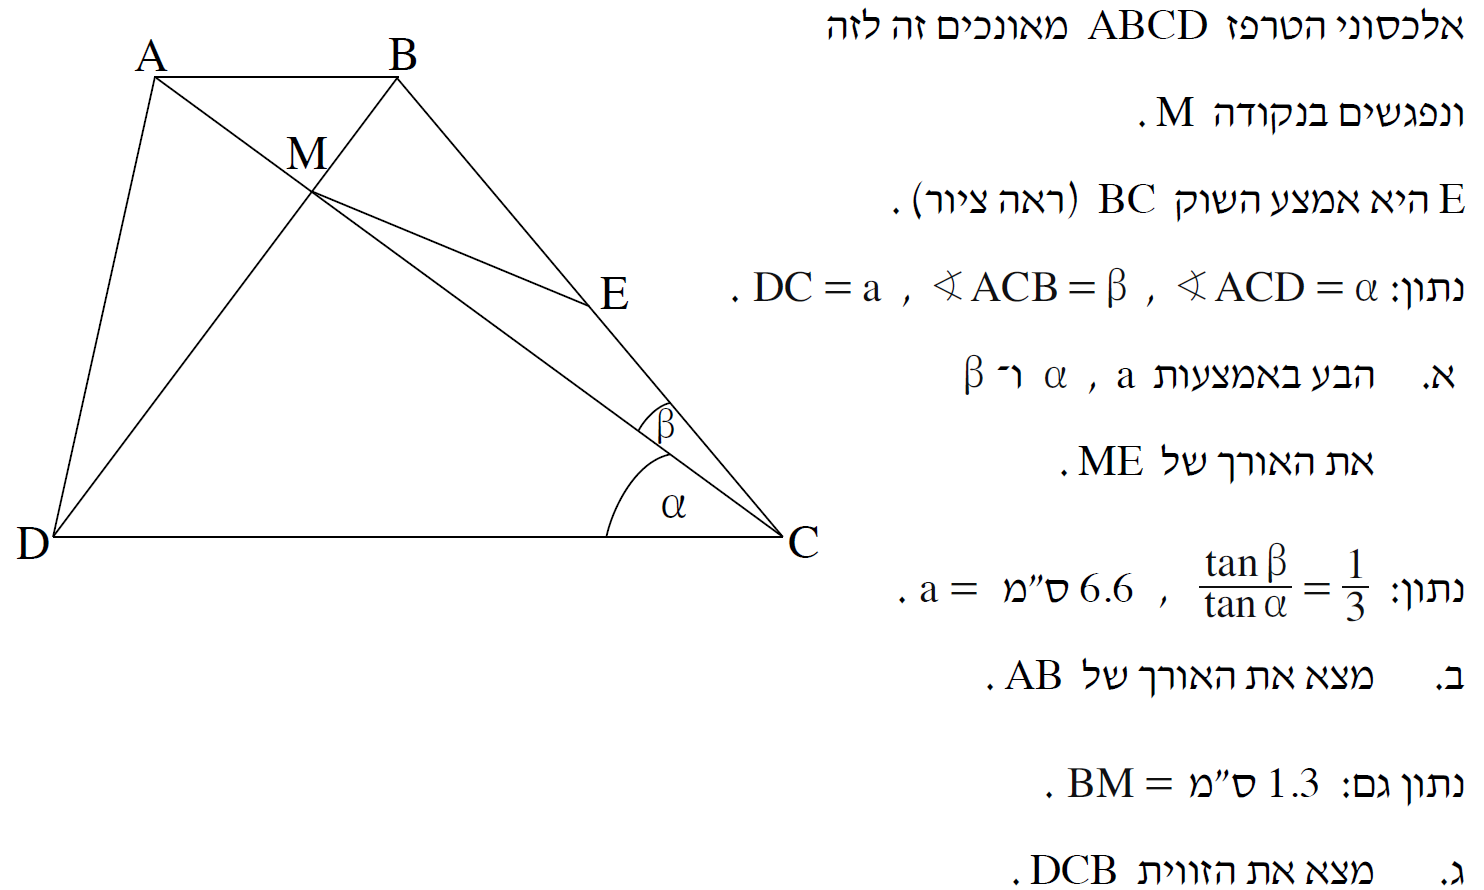
\includegraphics[width=.85\textwidth]{winter-2015-5}
\end{center}

\vspace{-2ex}


נמסן את הצלעות בתרשים.
\begin{center}
\selectlanguage{english}
\begin{tikzpicture}[scale=1.2]
\draw[thick] (0,0) coordinate (D) node[left] {$D$} -- node[below] {$a$} (6,0) coordinate (C) node[right] {$C$};
\draw[thick,name path=ca] (C) -- +(144:7) coordinate (A) node[left] {$A$};
\draw[thick,name path=db] (D) -- +(54:5.1) coordinate (B) node[right] {$B$};
\draw[thick] (D) -- (A) -- node[above] {$d$} (B) -- (C);
\path[name intersections={of=ca and db,by=M}];
\fill (A) node[below right,xshift=10pt] {$\alpha$} circle(1.5pt);
\fill (B) circle(1.5pt);
\fill (C) node[above left,xshift=-12pt] {$\alpha$} node[above left,xshift=-29pt,yshift=28pt] {$\beta$}  circle(1.5pt);
\fill (D) circle(1.5pt);
\fill (M) node[left,xshift=-2pt,yshift=-2pt] {$M$} circle(1.5pt);
\draw[rotate=-126] (M) rectangle +(8pt,8pt);
\coordinate (E) at ($(B) ! .5 ! (C) $);
\fill (E) node[right] {$E$} circle(1.5pt);
\draw[thick] (M) -- node[above] {$c/2$} (E);
\path (B) -- node[right] {$c/2$} (E) -- node[right] {$c/2$} (C);
\path (M) -- node[below] {$b$} (C);
\path (M) -- node[above] {$e$} (B);
\path (D) -- node[above] {$f$} (M);
\end{tikzpicture}
\end{center}

\vspace{-2ex}

\textbf{סעיף א}

$\triangle BMC$
ישר זווית ונתון ש-%
$ME$
הוא תיכון ליתר. לפי משפט 
$86$
"במשולש ישר זווית התיכון ליתר שווה למחצית היתר",
$ME=c/2$.
לפי ההגדרות של הפונקציות הטריגונומרטיות:

\vspace{-6ex}

\erh{12pt}
\begin{equationarray*}{rcl}
\cos \beta &=& \frac{b}{c}\\
\cos \alpha &=& \frac{b}{a}\\
ME &=& \frac{c}{2} = \frac{b}{2\cos\beta}\\
&=& \frac{a\cos\alpha}{2\cos\beta}\,.
\end{equationarray*}

\np

\textbf{סעיף ב}

למשולשים
$\triangle AMB, \triangle CMB$
צעל משותף
$MB=e$.
לפי ההגדרות של הפונקציות הטריגונומרטיות:

\vspace{-4ex}

\erh{12pt}
\begin{equationarray*}{rcl}
\tan \beta &=& \frac{e}{b}\\
\sin \alpha &=& \frac{e}{d}\\
AB = d &=& \frac{e}{\sin\alpha}=\frac{b\tan \beta}{\sin\alpha}\\
&=& \frac{a \cos\alpha\tan\beta}{\sin\alpha}=\frac{a\tan\beta}{\tan\alpha}\\
&=& 6.6\cdot\frac{1}{3} = 2.2\,.
\end{equationarray*}

\vspace{-3ex}

הוכחת אחרת משתמשת במשולשים דומים. 
$\angle BAM = \angle MCD = \alpha$
לפי זוויות מתחלפות, ו-%
$\triangle ABM \sim \triangle DMC$:

\vspace{-6ex}


\erh{12pt}
\begin{equationarray*}{rcl}
\tan \beta &=& \frac{e}{b}\\
\tan \alpha &=& \frac{f}{b}\\
\frac{e}{f}&=&\frac{\tan \beta}{\tan \alpha} =\frac{1}{3}\\
\frac{d}{a}&=& \frac{e}{f} =\frac{1}{3}\\
AB = d&=& \frac{6.6}{3}=2.2\,.
\end{equationarray*}

\vspace{-4ex}

\textbf{סעיף ג}

ממשפט פיתגורס
$b= \sqrt{a^2-f^2}=5.32$,
ו:
\erh{12pt}
\begin{equationarray*}{rcl}
\tan \beta &=& \frac{e}{b} = \frac{1.3}{5.32}=0.2444\\
\beta &=& 13.73\\
\tan \alpha &=& 3\tan\beta = 0.7331\\
\alpha &=& 36.24\\
\angle DCB &=& \alpha + \beta = 49.97\,.
\end{equationarray*}



%%%%%%%%%%%%%%%%%%%%%%%%%%%%%%%%%%%%%%%%%%%%%%%%%%%%%%%%%%%%%%

\np

\section{קיץ תשע"ד מועד ב}

\begin{center}
\selectlanguage{english}
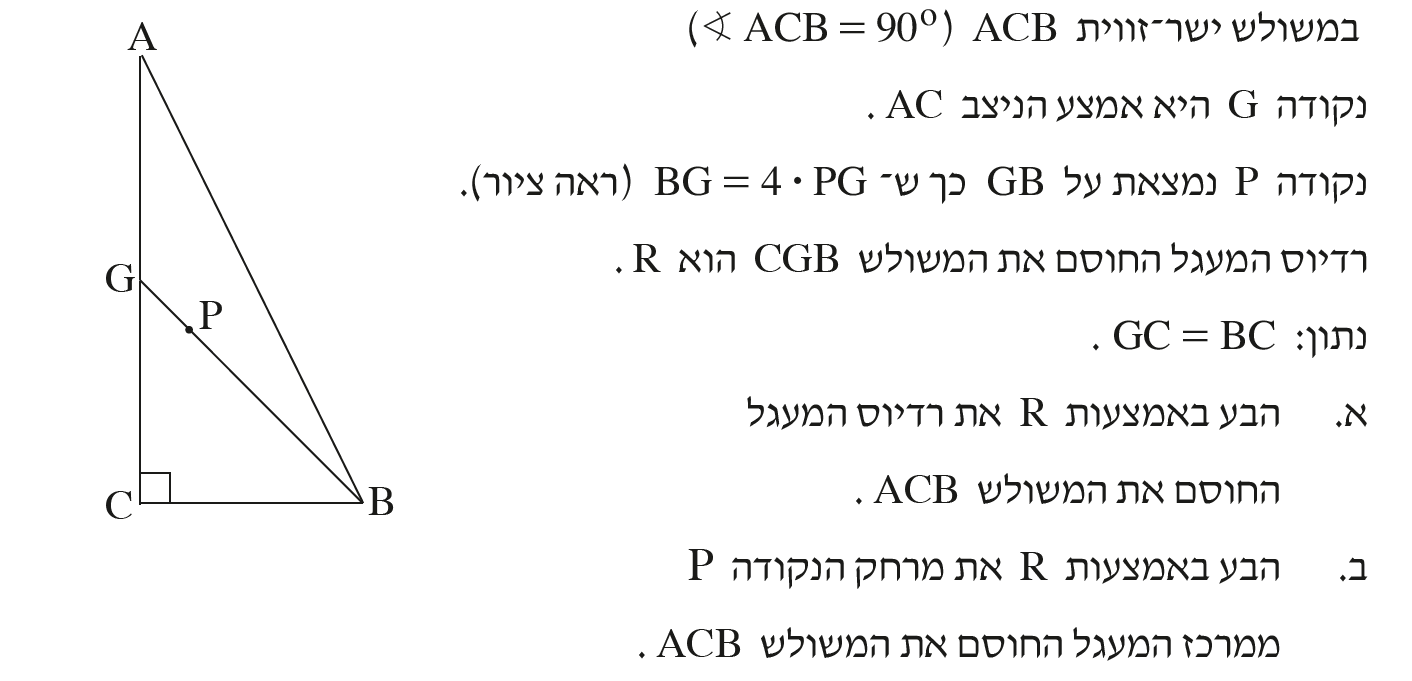
\includegraphics[width=\textwidth]{summer-2014b-5}
\end{center}

\vspace{-2ex}

מצאתי ששאלה זו קשה יחסית לשאלות אחרות בטריגונטמטריה. אתן שתי הוכחות לסעיף ב.

נסמן
$=R,M$
מרכז המעגל החוסם את
$\triangle CGB$
והרדיוס שלו, ו-%
$=R',M'$
מרכז המעגל החוסם את
$\triangle ACB$
והרדיוס שלו. שימו לב שבתרשים הנקודות
$M,M'$
נמצאות על הצלעות
$GB, AB$,
אבל אנו חייבים להוכיח את הטענה אם רוצים להשתמש בה.
\begin{center}
\selectlanguage{english}
\begin{tikzpicture}[scale=.75]
\draw[thick] (0,0) coordinate (C) -- node[below] {$a$} (4,0) coordinate (B) -- (0,8) coordinate (A) -- cycle;
\coordinate (G) at (0,4);
\path (C) -- node[left] {$a$} (G) -- node[left] {$a$} (A);
\draw[thick] (B) -- (G);
\coordinate (P) at ($(G)!.25!(B)$);
\fill (B) node[right] {$B$} circle(1.5pt);
\fill (A) node[above] {$A$} circle(1.5pt);
\fill (C) node[left] {$C$} circle(1.5pt);
\fill (G) node[left] {$G$} circle(1.5pt);
\fill (P) node[above,yshift=2pt] {$P$} circle(1.5pt);
\tkzCircumCenter(A,B,C)\tkzGetPoint{M1}
\tkzDrawCircle[thick,dotted,name path=circle](M1,A)
\tkzCircumCenter(C,G,B)\tkzGetPoint{M2}
\tkzDrawCircle[thick,dotted,name path=circle](M2,B)
\fill (M1) node[right] {$M'$} circle(1.5pt);
\fill (M2) node[left] {$M$} circle(1.5pt);
\draw (C) rectangle +(8pt,8pt);
\end{tikzpicture}
\end{center}

\vspace{-14ex}


\textbf{סעיף א}

נשתמש בחוק הסינוסים ובמשפט פיתגורס, תחילה עבור
$\triangle CGB$:
\[
R=\frac{BG}{2\sin 90}=\frac{BG}{2}=\frac{\sqrt{a^2+a^2}}{2}=\frac{a}{\sqrt{2}}\,,
\]
ואחר כך עבור
$\triangle ACB$:
\[
R'=\frac{AB}{2\sin 90}=\frac{AB}{2}=\frac{\sqrt{a^2+(2a)^2}}{2}=\left(\frac{\sqrt{5}}{2}\right)a=\left(\frac{\sqrt{5}}{2}\right)\sqrt{2}R=\sqrt{\frac{5}{2}}R\,.
\]

\np

\textbf{סעיף ב}

$M'$,
מרכז המעגל החוסם את
$\triangle ACB$,
הוא נקודת החיתוך של האנכים האמצעיים
$GM'\perp AC$
ו-%
$M'H\perp BC$.
$CH=HB=\displaystyle\frac{a}{2}$.

\vspace{-2ex}

\begin{center}
\selectlanguage{english}
\begin{tikzpicture}[scale=1.4]
\clip (-.5,-1) rectangle +(5,5.4);
\draw[thick] (0,0) coordinate (C) -- (4,0) coordinate (B) -- (0,8) coordinate (A) -- cycle;
\coordinate (G) at (0,4);
\path (C) -- node[left] {$a$} (G) -- node[left] {$a$} (A);
\draw[thick] (B) -- (G);
\coordinate (P) at ($(G)!.25!(B)$);
\fill (B) node[right] {$B$} circle(1.5pt);
\fill (A) node[above] {$A$} circle(1.5pt);
\fill (C) node[left] {$C$} circle(1.5pt);
\fill (G) node[left] {$G$} circle(1.5pt);
\fill (P) node[below,xshift=-2pt,yshift=-2pt] {$P$} circle(1.5pt);
\tkzCircumCenter(A,B,C)\tkzGetPoint{M1}
\tkzCircumCenter(C,G,B)\tkzGetPoint{M2}
\fill (M1) node[right] {$M'$} circle(1.5pt);
\fill (M2) node[left,xshift=-2pt,yshift=-2pt] {$M$} circle(1.5pt);
\draw (C) rectangle +(8pt,8pt);
\draw (G) rectangle +(8pt,8pt);
\draw[thick] (P) -- node[above,xshift=-2pt] {$z$} (M1);
\coordinate (H) at (M1 |- B);
\fill (H) node[below] {$H$} circle(1.5pt);
\draw[thick,dashed] (G) -- (M1) -- (H);
\draw (H) rectangle +(8pt,8pt);
\path (G) -- node[below,xshift=-4pt,yshift=2pt] {$x$} (P) -- node[below,xshift=-4pt,yshift=2pt] {$x$} (M2) -- node[below,xshift=-4pt,yshift=2pt] {$2x$} (B);
\path (C) -- node[below] {$a/2$} (H) -- node[below] {$a/2$} (B);
\path (M1) -- node[right] {$y$} (M2) -- node[left] {$a/2$} (H);
\end{tikzpicture}
\end{center}

\vspace{-5ex}

אם נמצא משולש שעבורו נוכל לחשב שני צלעות והזווית הכלואה ביניהם, נוכל להשתמש בחוק הקוסינוסים. ננסה את
$\triangle MPM'$.
$CG\|MH$
ולכן לפי משפט 
$91$
"משפט תאלס המורחב: ישר המקביל לאחת מצלעות המשולש חותך את שתי הצלעות האחרות או את המשכיהן בקטעים פרופורציוניים":
\[
\frac{GC}{MH}=\frac{CB}{HB}=\frac{a}{a/2}=2\,,
\]
ו-%
$MH=\displaystyle\frac{a}{2}$.
אבל
$GCHM'$
הוא מלבן, ולכן:
\[
y=MM'=M'H-MH=GC-MH=a-\frac{a}{2}=\frac{a}{2}=\frac{1}{2}\cdot \sqrt{2}R=\frac{R}{\sqrt{2}}\,.
\]
שוב לפי משפט תאלס המורחב:
\[
\frac{GB}{MB}=\frac{GC}{MH}=2\,,
\]
ו-%
$GM=MB$
שנסמן
$2x$.
נתון
$GB=4\cdot PG$,
כך ש-%
$PG=\displaystyle\frac{1}{4} (2x+2x)=x$.
לבסוף,
$PM=4x-(2x)-x=x$.
את
$x$
ניתן לחשב לפי משפט פיתגורס ב-%
$\triangle CGB$:

\vspace{-6ex}

\erh{12pt}
\begin{equationarray*}{rcl}
(4x)^2&=&a^2+a^2\\
x&=&\frac{1}{\sqrt{8}}a=\frac{1}{\sqrt{8}}\cdot\sqrt{2}R=\frac{R}{2}\,.
\end{equationarray*}

$\triangle MHB$
הוא משלוש ישר-זווית, כך ש-%
$\angle BMH=45$
ו-%
$\angle PMM'=45$
לפי זוויות קודקודיות.

כעת יש לנו מספיק נתונים להשתמש בחוק הקוסינוסים. נסמן
$z=PG$:

\np

\erh{14pt}
\begin{equationarray*}{rcl}
z^2&=&x^2+y^2-2xy\cos \angle PMM'\\
&=&\left(\frac{R}{2}\right)^2+\left(\frac{R}{\sqrt{2}}\right)^2 - 2\left(\frac{R}{2}\right)\left(\frac{R}{\sqrt{2}}\right)\cos 45\\
&=& R^2\left(\frac{1}{4}+\frac{1}{2}-\frac{1}{\sqrt{2}}\cdot \frac{\sqrt{2}}{2}\right)=\frac{R^2}{4}\\
z&=&\frac{R}{2}\,.
\end{equationarray*}

\vspace{-4ex}

\begin{center}
*\ *\ *
\end{center}

פתרון אחר משתמש בחוק הקוסינוסים על 
$\triangle PM'B$.
$GM'$,
האנך האמצעי לצלע 
$AC$
חותך את
$AB$
ב-%
$M'$
)בלי להסתמך על 
$M'$
כמרכז המעגל החסום את 
$\triangle ACB$(.
$GM'\|CB$
ולכן לפי משפט תאלס )הרגיל(
\[
\frac{AG}{GC}=\frac{AM'}{M'B}\,,
\]
ונסמן
$y=AM'=M'B$.

\begin{center}
\selectlanguage{english}
\begin{tikzpicture}[scale=.9]
\draw[thick] (0,0) coordinate (C) -- node[below] {$a$} (4,0) coordinate (B) -- (0,8) coordinate (A) node[below,xshift=6pt,yshift=-20pt] {$\alpha$} -- cycle;
\coordinate (G) at (0,4);
\path (C) -- node[left] {$a$} (G) -- node[left] {$a$} (A);
\draw[thick] (B) -- (G);
\coordinate (P) at ($(G)!.25!(B)$);
\fill (B) node[right] {$B$} circle(1.5pt);
\fill (A) node[above] {$A$} circle(1.5pt);
\fill (C) node[left] {$C$} circle(1.5pt);
\fill (G) node[left] {$G$} node[below left,xshift=-6pt,yshift=-4pt] {$45$} circle(1.5pt);
\draw[->] ($(G)+(-8pt,-14pt)$) -- +(14pt,0);
\path (G) -- node[left,near end] {$x$} (P);
\fill (P) node[below,yshift=-2pt] {$P$} circle(1.5pt);
\tkzCircumCenter(A,B,C)\tkzGetPoint{M1}
\tkzCircumCenter(C,G,B)\tkzGetPoint{M2}
\fill (M1) node[right] {$M'$} circle(1.5pt);
\draw (C) rectangle +(8pt,8pt);
\draw (G) rectangle +(8pt,8pt);
\draw[thick,dashed] (G) -- (M1);
\draw[thick] (P) -- (M1);
\path (A) -- node[right] {$y$} (M1) -- node[right] {$y$} (B);
\node at ($(B)+(15pt,20pt)$) {$\beta$};
\draw[->] ($(B)+(10pt,20pt)$) -- +(-26pt,0);
\path (P) -- node[below,near start,yshift=-2pt] {$3x$} (B);
\path (P) -- node[above,near start] {$z$} (M1);
\end{tikzpicture}
\end{center}

\vspace{-17ex}

ולפי פיתגורס ב-%
$\triangle GCB$:
\erh{12pt}
\begin{equationarray*}{rcl}
(4x)^2 &=& a^2+a^2\\
x&=&\frac{1}{\sqrt{8}}a=\frac{1}{\sqrt{8}}\cdot\sqrt{2}R=\frac{R}{2}\,.
\end{equationarray*}

\np

לפי פיתגורס ב-%
$\triangle ACB$:
\erh{12pt}
\begin{equationarray*}{rcl}
(2y)^2&=&(2a)^2+a^2\\
y&=&\frac{\sqrt{5}}{2}a=\frac{\sqrt{5}}{2}\cdot \sqrt{2}R=\sqrt{\frac{5}{2}}R\,.
\end{equationarray*}
נחשב את הזוויות
$\alpha,\beta$:
\erh{14 pt}
\begin{equationarray*}{rcl}
\sin \alpha &=& \frac{a}{2y}= \frac{\sqrt{2}R}{2\sqrt{(5/2)}R} = \sqrt{\frac{1}{5}}\\
\alpha &=& 26.57\\
\beta&=& 180-\angle AGB-\alpha=180-135-26.57=18.43\,.
\end{equationarray*}
נשמתש בחוק הקוסינוסים ב-%
$\triangle PM'B$:
\erh{16pt}
\begin{equationarray*}{rcl}
z^2&=&(3x)^2 + y^2 - 2\cdot 3x\cdot y \cdot \cos \beta\\
&=&\left(\frac{3R}{2}\right)^2 + \left(\sqrt{\frac{5}{2}}R\right)^2 - 2\cdot \frac{3R}{2} \cdot \sqrt{\frac{5}{2}} \cdot 0.9487\\
&=&0.25R^2\\
z&=&\frac{R}{2}\,.
\end{equationarray*}


אני מעדיף את הפתרון הראשון. אמנם התרשים מעט יותר מסובך אבל החישובים הרבה יותר פשוטים.



\np

\section{קיץ תשע"ד מועד א}

%%%%%%%%%%%%%%%%%%%%%%%%%%%%%%%%%%%%%%%%%%%%%%%%%%%%%%%%%%%%%%

\begin{center}
\selectlanguage{english}
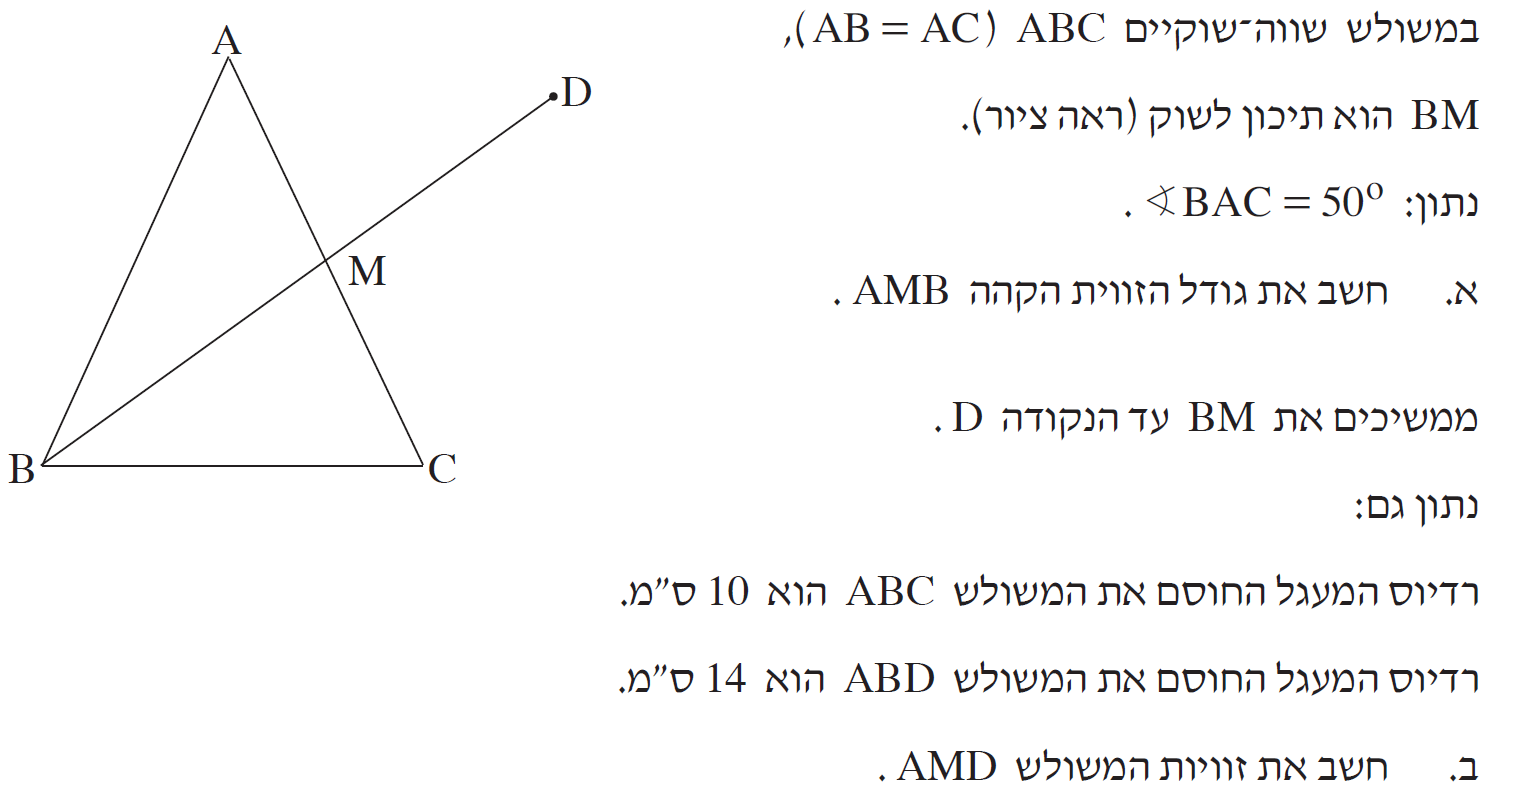
\includegraphics[width=\textwidth]{summer-2014a-5}
\end{center}

\vspace{-2ex}


נסמן
$\alpha=\angle AMB$.
נתון 
$\angle BAC=50$
ובמשולש שווה-שוקיים:
\[
\angle ABC=\angle ACB=(180-50)/2=65\,.
\]
נחשב
$\angle ABM=180-50-\alpha=130-\alpha$.

\vspace{-2ex}

\begin{center}
\selectlanguage{english}
\begin{tikzpicture}[scale=.9]
\draw[thick] (0,0) coordinate (B) -- (5,0) coordinate (C);
\draw[thick] (B) -- node[left] {$a$} (2.5,6) coordinate (A);
\draw[thick,name path=ac] (A) -- (C);
\fill (B) node[below left] {$B$} node[above right,xshift=4pt] {$65$} circle(1.5pt);
\fill (A) node[above] {$A$} node[below,yshift=-16pt] {$50$} circle(1.5pt);
\fill (C) node[below right] {$C$} node[above left,xshift=-4pt] {$65$} circle(1.5pt);
\coordinate (M) at ($(A)!.5!(C)$);
\fill (M) node[below right,xshift=4pt,yshift=2pt] {$M$} node[left,yshift=2pt] {$\alpha$}  circle(1.5pt);
\draw[thick] (B) -- (M);
\path (A) -- node[right] {$a/2$} (M);
\path (M) -- node[right] {$a/2$} (C);
\node at ($(B)+(-25pt,25pt)$) {$130\!-\!\alpha$};
\draw[->] ($(B)+(0,25pt)$) -- +(18pt,0);
\end{tikzpicture}
\end{center}

\vspace{-3ex}


\textbf{סעיף א}


נחפש משולש שעליו אפשר להפעיל את חוק הסינוסים. נתון ש-%
$BM$
הוא תיכון ל-%
$AC$.
נסמן את 
$AB,AM$
עם הנעלם
$a$,
ונפעיל את משפט הסינוים על
$\triangle ABM$.

\vspace{-3ex}


\erh{12pt}
\begin{equationarray*}{rcl}
\frac{a}{\sin\alpha}&=&\frac{a/2}{\sin(130-\alpha)}\\
\sin \alpha &=& 2\sin(130-\alpha)\\
&=&2\sin 130\cos \alpha - 2\sin\alpha \cos 130
\end{equationarray*}

\np

\erh{12pt}
\begin{equationarray*}{rcl}
&=&1.53\cos\alpha + 1.29\sin\alpha\\
\tan \alpha &=& \frac{-1.53}{0.29}\\
\alpha&=&-79.27^\circ = 100.73^\circ\approx 101^\circ\,.
\end{equationarray*}
בהמשך נעבוד עם קירובים למעלה שלמה.

\textbf{סעיף ב}

\begin{center}
\selectlanguage{english}
\begin{tikzpicture}[scale=.9]
\clip(-2,-1.1) rectangle +(11,7.6);
\draw[thick] (0,0) coordinate (B) -- (5,0) coordinate (C);
\draw[thick] (B) -- node[left] {$a$} (2.5,6) coordinate (A);
\draw[thick,name path=ac] (A) -- (C);
\fill (B) node[below left] {$B$} circle(1.5pt);
\fill (A) node[above] {$A$} circle(1.5pt);
\fill (C) node[below right] {$C$} node[above left,xshift=-4pt] {$65$}circle(1.5pt);
\coordinate (M) at ($(A)!.5!(C)$);
\fill (M) node[below right,xshift=4pt,yshift=2pt] {$M$} node[left,yshift=2pt] {$101$} node[above,xshift=3pt,yshift=7pt] {$79$}  circle(1.5pt);
\draw[thick] (B) -- ($(B)!1.8!(M)$) coordinate (D);
\fill (D) node[right] {$D$} node[below left,xshift=-12pt,yshift=2pt] {$\beta$} circle(1.5pt);
\path (A) -- (M);
\path (M) -- (C);
\tkzCircumCenter(A,B,C)\tkzGetPoint{C1}
\tkzDrawCircle[thick,dotted,name path=circle](C1,A)
\tkzCircumCenter(A,B,D)\tkzGetPoint{D1}
\tkzDrawCircle[thick,dotted,name path=circle](D1,A)
\draw[thick,dashed] (A) -- (D);
\end{tikzpicture}
\end{center}

חישבנו
$\angle AMD=79^\circ$
בסעיף הקודם. נצטרך לחשב אחת מ-%
$\angle MAD,\angle ADM$,
והזווית השלישית תתקבל מסכום הזוויות במשולש. מהתרשים אנו רואים שהצלע 
$AB$
מול הזווית
$\beta=\angle ADM$
הוא באורך
$a$,
ו-%
$AB$
הוא גם צלע מול
$\angle AMB=101$.
לפי חוק הסינוסים ב-%
$\angle ACB$, $\angle ADB$:

\vspace{-4ex}

\erh{10pt}
\begin{equationarray*}{rcl}
2R_{ABC}&=&\frac{a}{\sin 65}=2\cdot 10\\
a &=& 18.126\\
2R_{ABD}&=&\frac{a}{\sin \beta}=\frac{18.126}{\sin \beta}=2\cdot 14\\
\beta &=& 40.34\,.
\end{equationarray*}
הזוויות של
$\triangle AMD$
הן )בקירוב למעלה שלמה(
$79^\circ, 40^\circ, 61^\circ$.


%%%%%%%%%%%%%%%%%%%%%%%%%%%%%%%%%%%%%%%%%%%%%%%%%%%%%%%%%%%%%%
\np

\section{חורף תשע"ד}

\begin{center}
\selectlanguage{english}
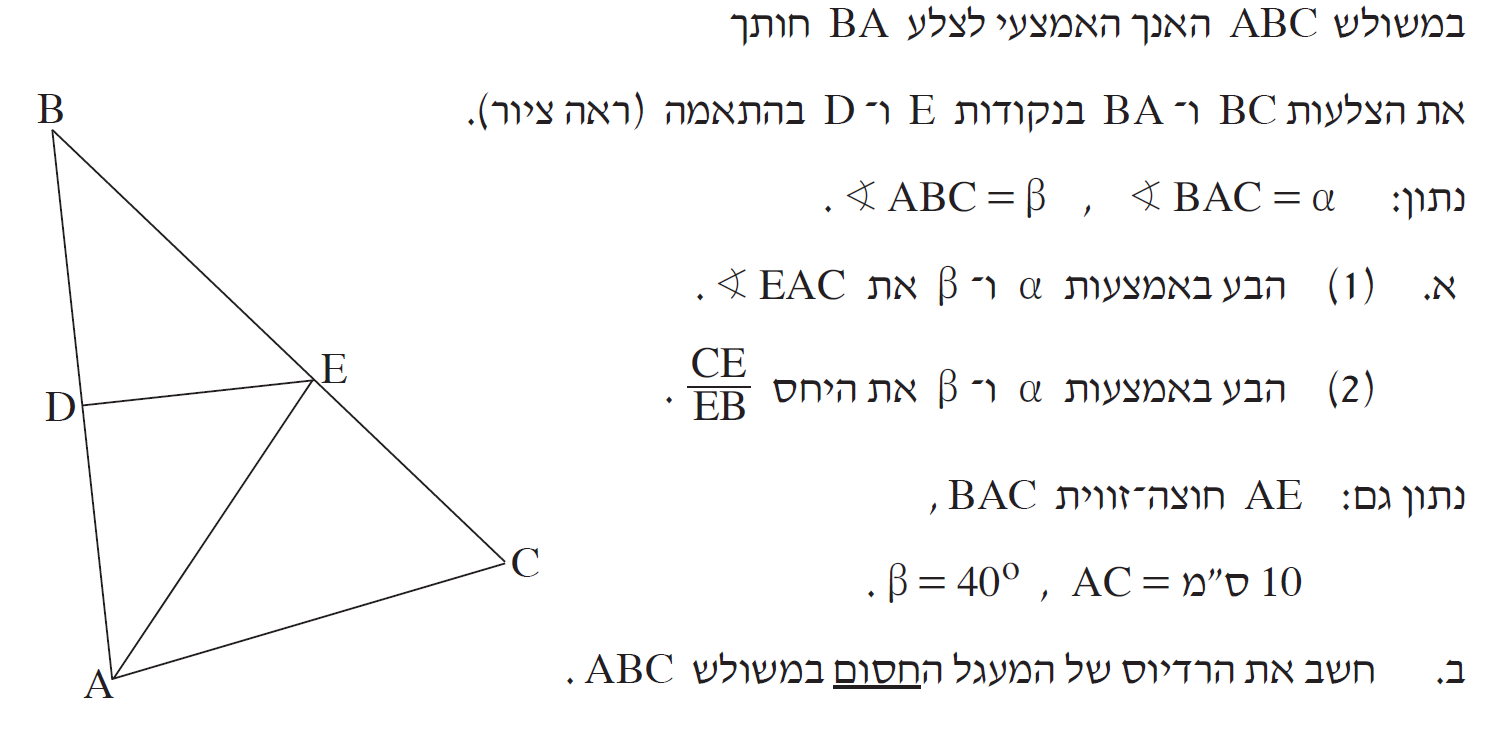
\includegraphics[width=.9\textwidth]{winter-2014-5}
\end{center}

\vspace{-2ex}

\textbf{סעיף א}

$(1)$
נתון ש-%
$DE$
הוא האנך האמצעי ל-%
$AB$,
ולכן
$\triangle AED\cong BED$
לפי צ.ז.צ. נסמן את שאר הזוויות לפי זוויות משלימות וסכום זוויות המשולש, כאשר קיצרנו
$\beta'=90-\beta$.
התשובה היא
$\angle EAC=\alpha-\beta$.

\vspace{-3ex}

\begin{center}
\selectlanguage{english}
\begin{tikzpicture}[scale=.85]
\draw[thick] (0,0) coordinate (A) -- (5,1) coordinate (C);
\draw[thick] (A) -- (100:8) coordinate (B);
\draw[thick,name path=bc] (B) -- (C);
\coordinate (D) at ($(A) ! .5 ! (B)$);
\fill (A) node[below left] {$A$} node[above right,xshift=10pt,yshift=14pt] {$\alpha$} node[above,xshift=4pt,yshift=20pt] {$\beta$} circle(1.5pt);
\fill (B) node[above] {$B$} node[below right,xshift=4pt,yshift=-16pt] {$\beta$} circle(1.5pt);
\fill (C) node[right] {$C$} node[above right,xshift=-4pt,yshift=6pt] {$180-(\alpha+\beta)$} circle(1.5pt);
\draw[->] ($(C)+(0pt,12pt)$) -- +(-14pt,-8pt);
\fill (D) node[left] {$D$} circle(1.5pt);
\path[name path=de] (D) -- +(10:4);
\path[name intersections={of=bc and de,by={E}}];
\fill (E) node[right] {$E$} node[above left,xshift=-8pt,yshift=-4pt] {$\beta'$} node[below left] {$\beta'$} node[below,xshift=4pt,yshift=-12pt] {$2\beta$}   circle(1.5pt);
\draw[thick] (D) -- (E);
\draw[thick,name path=ae] (A) -- (E);
\path (A) -- node[left] {$a$} (D);
\path (D) -- node[left] {$a$} (B);
\path (C) -- node[right] {$c$} (E);
\path (E) -- node[right,xshift=2pt] {$b$} (B);
\path (E) -- node[right] {$b$} (A);
\draw[rotate=10] (D) rectangle +(7pt,7pt);
\draw[very thick] ($(A)+(10:10mm)$) arc[start angle=25,end angle=101,radius=10mm];
\end{tikzpicture}
\end{center}

\vspace{-2ex}

$(2)$
נסמן 
$BE=b$,$EC=c$.
השאלה מבקשת את היחס
$\displaystyle\frac{c}{b}$.
מהתרשים נראה ש-%
$\angle BAC=\alpha=90$
ונוכל להשתמש במשפט תאלס, אבל אי אפשר להסתמך על התרשמות מהתרשים. הראנו ש-%
$\triangle AED\cong BED$,
כך ש-%
$AE=BE=b$,
ונוכל להשתמש במשפט הסינוסים ב-%
$\triangle AEC$:

\vspace{-6ex}

\erh{12pt}
\begin{equationarray*}{rcl}
\frac{c}{\sin (\alpha-\beta)}&=&\frac{b}{\sin(180-(\alpha+\beta))}\\
\frac{c}{b}&=&\frac{\sin (\alpha-\beta)}{\sin (\alpha+\beta)}\,.
\end{equationarray*}

\vspace{-2ex}

\np

\textbf{סעיף ב}

המשפט הרלוונטי הוא
$49$
"שלושת חוצי הזוויות של משולש נחתכים בנקודה אחת, שהיא מרכז המעגל החסום במשולש". נתון חוצה זווית 
$AE$
ב-%
$A$.
נבנה חוצה זווית שני. ננסה ב-%
$C$
כי ידוע
$AC=10$
ונוכל להשתמש במשפט הסינוסים ב-%
$\triangle ACF$,
כאשר 
$F$ 
היא נקודת החיתוך עם חוצה הזוויות 
$AE$,
ולכן היא המרכז של המעגל החסום.

נתון ש-%
$\beta=40$
וזה מאפשר לנו להשלים זוויות בתרשים:

\begin{center}
\selectlanguage{english}
\begin{tikzpicture}[scale=.85]
\draw[thick] (0,0) coordinate (A) -- (5,1) coordinate (C);
\draw[thick] (A) -- (100:8) coordinate (B);
\draw[thick,name path=bc] (B) -- (C);
\coordinate (D) at ($(A) ! .5 ! (B)$);
\fill (A) node[below left] {$A$} node[above right,xshift=10pt,yshift=10pt] {$40$} node[above,xshift=3pt,yshift=18pt] {$40$} circle(1.5pt);
\fill (B) node[above] {$B$} node[below right,xshift=3pt,yshift=-18pt] {$40$} circle(1.5pt);
\fill (C) node[right] {$C$} node[left,xshift=-14pt,yshift=2pt] {$30$} node[above left,xshift=-16pt,yshift=8pt] {$30$} circle(1.5pt);
\fill (D) node[left] {$D$} circle(1.5pt);
\path[name path=de] (D) -- +(10:4);
\path[name intersections={of=bc and de,by={E}}];
\fill (E) node[right] {$E$} node[above left,xshift=-8pt,yshift=-4pt] {$50$} node[below left,xshift=-3pt,yshift=-2pt] {$50$} node[below,xshift=4pt,yshift=-12pt] {$80$}   circle(1.5pt);
\draw[thick] (D) -- (E);
\draw[thick,name path=ae] (A) -- (E);
\path (A) -- node[left] {$a$} (D);
\path (D) -- node[left] {$a$} (B);
\path (C) -- node[right] {$c$} (E);
\path (E) -- node[right,xshift=2pt] {$b$} (B);
\path (E) -- node[right,xshift=4pt,yshift=10pt] {$b$} (A);
\path (A) -- node[below] {$10$} (C);
\draw[rotate=10] (D) rectangle +(7pt,7pt);
\path[name path=cf] (C) -- +(160:5);
\path[name intersections={of=ae and cf,by={F}}];
\fill (F) node[left] {$F$} node[below,xshift=8pt,yshift=-8pt] {$110$} circle(1.5pt);
\draw[thick] (C) -- node[above] {$x$} (F);
\end{tikzpicture}
\end{center}

\vspace{-3ex}

לפי משפט הסינוסים:
\erh{14pt}
\begin{equationarray*}{rcl}
\frac{x}{\sin 40}&=&\frac{10}{\sin 110}\\
x &=& 6.84\,.
\end{equationarray*}
\textbf{לא לעצור כאן!}
השאלה מבקשת את הרדיוס של המעגל החסום ולא המרחק אל מרכז המעגל. 

נוריד אנך מ-%
$F$
לצלע 
$AC$
ולחשב:
$r=x\sin 30 = 3.42$.

כדי להראות את המעגל החסום, ציירתי תרשים חדש עם ערכי זוויות מדוייקים:
\begin{center}
\selectlanguage{english}
\begin{tikzpicture}[scale=.9]
\clip(-1.1,-.6) rectangle +(8.5,5.3);
\coordinate (A) at (0,0);
\draw[thick] (A) -- +(90:8) coordinate (B);
\path[name path=bc] (B) -- +(-50:10);
\path[name path=ac] (A) -- +(10:7);
\path[name intersections={of=ac and bc,by={C}}];
\draw[thick] (A) -- (C) -- (B);
\fill (B) node[above] {$B$};
\fill (A) node[below left] {$A$} node[above right,xshift=10pt,yshift=4pt] {$40$} circle(1.5pt);
\fill (C) node[right] {$C$} node[left,xshift=-14pt,yshift=2pt] {$30$} circle(1.5pt);
\path[name path=af] (A) -- +(50:5);
\path[name path=cf] (C) -- +(160:6);
\path[name intersections={of=af and cf,by={F}}];
\fill (F) node[above] {$F$} circle(1.5pt);
\draw[thick] (A) -- (F) -- node[above,near start] {$x$} (C);
\coordinate (G) at ($(A)!(F)!(C)$);
\draw[very thick,dashed]  (G) -- node[left] {$r$} (F);
\draw[rotate=10] (G) rectangle +(7pt,7pt);
\fill (G) circle(1.5pt);
\node[draw,very thick,dotted,circle through=(G)] at (F) {};
\end{tikzpicture}
\end{center}

\section{חורף תשע"ד )שאלה
$6$(}

\textbf{בבחינה זו היו שלוש שאלות בפרק השני.}

\begin{center}
\selectlanguage{english}
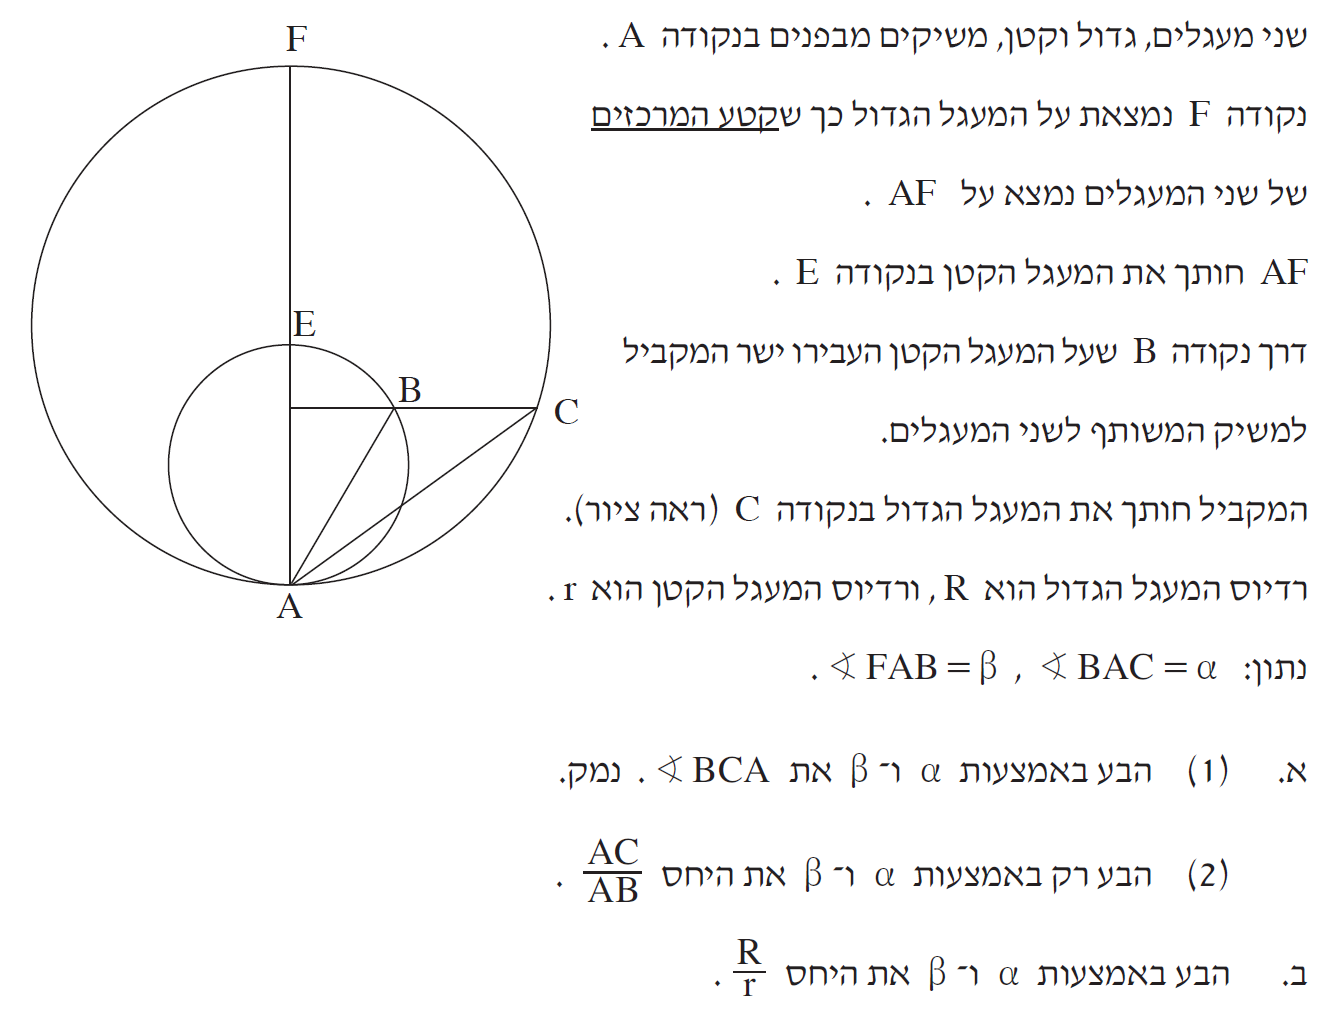
\includegraphics[width=.95\textwidth]{winter-2014-6}
\end{center}

\vspace{-2ex}

\begin{center}
\selectlanguage{english}
\begin{tikzpicture}[scale=.85]
\coordinate (O) at (0,0);
\coordinate (A) at (0,-4);
\coordinate (F) at (0,4);
\fill (A) circle(1.5pt) node[below] {$A$} node[above right,yshift=18pt,xshift=11pt] {$\alpha$} node[above,yshift=15pt,xshift=6pt] {$\beta$};
\fill (F) circle(1.5pt) node[above] {$F$};
\node[draw,thick,circle through=(A),name path=big-circle] (circle) at (O) {};
\node[draw,thick,circle through=(A),name path=small-circle] (circle) at (0,-2.1) {};
\draw[thick,name path=diameter] (A) -- (F);
\path[name intersections={of=diameter and small-circle,by={E}}];
\fill (E) circle(1.5pt) node[above left] {$E$};

\path[name path=ab] (A) -- +(65:5);
\path[name intersections={of=ab and small-circle,by={B}}];
\draw[thick] (A) -- (B);
\fill (B) circle(1.5pt) node[above right] {$B$};
\coordinate (D) at (A|-B);
\fill (D) circle(1.5pt) node[left] {$D$};
\path[name path=dc] (D) -- ($(D)!3!(B)$);
\path[name intersections={of=dc and big-circle,by={C}}];
\draw[thick] (D) -- (C);
\fill (C) circle(1.5pt) node[right] {$C$} node[below left,xshift=-12pt] {$\gamma$};
\draw[thick] (A) -- (C);
\draw[thick,rotate=-90] (D) rectangle +(7pt,7pt);
\node at (1.8,1.5) {$\gamma = 90\!-\!(\alpha\!+\!\beta)$};
\end{tikzpicture}
\end{center}

בפתרון השאלה נשתמש לעתים קורבות בקשר בין סינוס לקוסינוס במשולש ישר זווית:

\np

\begin{center}
\selectlanguage{english}
\begin{minipage}{.4\textwidth}
\begin{tikzpicture}
\draw[thick] (0,0) -- node[below] {$a$} (4,0) -- node[right] {$b$} (4,3) -- node[above] {$c$} cycle;
\coordinate (B) at (4,0);
\draw[thick,rotate=90] (B) rectangle +(7pt,7pt);
\node[above right,xshift=16pt] at (0,0) {$90-\theta$};
\node[below left,xshift=1pt,yshift=-6pt] at (4,3) {$\theta$};
\end{tikzpicture}
\end{minipage}
\begin{minipage}{.4\textwidth}
\[
\begin{array}{l}
\sin\theta = \displaystyle\frac{a}{c} = \cos(90-\theta)\\
\cos\theta = \displaystyle\frac{b}{c} = \sin(90-\theta)\\
\mbox{}
\end{array}
\]
\end{minipage}
\end{center}

\vspace{-4ex}

\textbf{סעיף א}

$(1)$
$\triangle DCA$ 
יישר זווית ולכן סכום הזזויות החדות שווה ל-%
$90$. $\angle BCA=\gamma=90-(\alpha+\beta)$.

$(2)$
$AD$
צלע של
$\triangle DCA$
וגם של
$\triangle DBA$.
נפעיל את חוק הסינוסים פעמיים:
\erh{12pt}
\begin{equationarray*}{rcl}
\frac{AB}{\sin 90}&=&\frac{AD}{\sin (90-\beta)}\\
AD&=&AB\cos \beta\\
\frac{AC}{\sin 90}&=&\frac{AD}{\sin \gamma}\\
AC&=&\frac{AB\cos\beta}{\sin(90-(\alpha+\beta))}\\
\frac{AC}{AB}&=&\frac{\cos\beta}{\cos(\alpha+\beta)}\,.
\end{equationarray*}
פתרון אחר מתקבל מהפעלת חוק שסינוסים פעם אחת על
$\triangle ABC$:
\erh{12pt}
\begin{equationarray*}{rcl}
\frac{AC}{\sin(180-\alpha-\gamma)}&=&\frac{AB}{\sin\gamma}\\
\frac{AC}{AB}&=&\frac{\sin(\alpha+\gamma)}{\cos(\alpha+\beta)}\\
&=&\frac{\sin(\alpha+90-(\alpha+\beta))}{\cos(\alpha+\beta)}=\frac{\cos\beta}{\cos(\alpha+\beta)}
\end{equationarray*}


\textbf{סעיף ב}

סביר שנצטרך להשתמש בתוצאה של הסעיף הקודם, לכן נחפש קשר בין הקווים 
$AB,AC$
לבין הרדיוסים. נחבר 
$B$
ל-%
$E$
ו-%
$C$
ל-%
$F$.
נקבל שני משולשים חסומים במעגלים וניתן להשתמש בנוסחה של חוק הסינוסים עם רדיוס. 

\np

\begin{center}
\selectlanguage{english}
\begin{tikzpicture}[scale=.7]
\coordinate (O) at (0,0);
\coordinate (A) at (0,-4);
\coordinate (F) at (0,4);
\fill (A) circle(2pt) node[below] {$A$} node[above right,yshift=18pt,xshift=11pt] {$\alpha$} node[above,yshift=15pt,xshift=6pt] {$\beta$};
\fill (F) circle(2pt) node[above] {$F$};
\node[draw,thick,circle through=(A),name path=big-circle] (circle) at (O) {};
\node[draw,thick,circle through=(A),name path=small-circle] (circle) at (0,-2.1) {};
\draw[thick,name path=diameter] (A) -- (F);
\path[name intersections={of=diameter and small-circle,by={E}}];
\fill (E) circle(2pt) node[above left] {$E$};

\path[name path=ab] (A) -- +(65:5);
\path[name intersections={of=ab and small-circle,by={B}}];
\draw[thick] (A) -- (B);
\fill (B) circle(2pt) node[above right] {$B$};
\coordinate (D) at (A|-B);
\path[name path=dc] (D) -- ($(D)!3!(B)$);
\path[name intersections={of=dc and big-circle,by={C}}];
\fill (C) circle(2pt) node[right] {$C$};
\draw[thick] (A) -- (C);
\draw[thick,rotate=155] (B) rectangle +(7pt,7pt);
\draw[thick,rotate=130] (C) rectangle +(7pt,7pt);
\draw[thick,dashed] (C) -- (F);
\draw[thick,dashed] (B) -- (E);
\end{tikzpicture}
\end{center}
פתרון אחר: נתון ש-%
$FA$
הוא קוטר )"קטע המרכזים"( של המגעל הגדול, ולכן 
$EA$
הוא קוטר של המעגל הקטן. זווית הנשענת על קוטר היא זווית ישרה, כך ש-%
$\triangle ACF,\triangle ABE$
הם ישר זווית, וניתן פשוט להשמתמש בהגדרת הפונקציות הטריגונומטריות:
\erh{14pt}
\begin{equationarray*}{rcl}
\cos \beta &=& \frac{AB}{2r}\\
\cos (\alpha+\beta) &=& \frac{AC}{2R}\\
\frac{R}{r}&=&\frac{AC}{2\cos(\alpha+\beta)}\cdot \frac{2\cos\beta}{AB}\\
&=&\frac{\cos^2\beta}{\cos^2(\alpha+\beta)}\,.
\end{equationarray*}

\np

\section*{המלצות: טריגונומטריה}

\addcontentsline{cot}{chapter}{המלצות: טריגונומטריה}


\begin{itemize}

\item
ראו נספח~%
\ref{a.unit-circle}
המסביר את החשיבות של מעגל היחידה בחישובים טריגונומטריים.

הנספח מציג איך לשחזר בקלות את הנוסחאות ל-%
$\sin 2\theta$, $\sin (180^\circ-\theta)$, $\sin (90^\circ-\theta)$,
ונוסאות דומות עבור קיסינוס.

\item
חשוב לצייר תרשימים 
\textbf{ברורים וגדולים}
עדיף עם סרגל ומחוגה. בתהליך הפתרון אנו מסמנים את המידע המצטבר על הזוויות והצלעות ויש לדאוג שיהיה מספיק מקום.

\item
כאשר לשאלה יש מספר סעיפים כדאי לצייר תרשימים נפרדים לכל סעיף תוך העלמת מידע לא רלוונטי לאותו סעיף.

\item
אני מעדיף לסמן זוויות עם אותיות יווניות כגון
$\alpha$,
ולא על ידי ציון שלושת הנקודות המגדירות אותה
$\angle ABC$,
כי קשה יותר לעקוב אחר הנקודות המגדירות את הזווית.

\item
השלימו זוויות ככל האפשר תוך שימוש בסכום הזוויות במשולש, ובזוויות משלימות. כדי להקל על החישובים אני משתמש בנעלמים נוספים כדי לקצר ביטויים, למשל,
$\gamma=180-(\alpha+\beta)$.

\item
שימו לב שאין עקביות בסימון 
$A,B,C,D$
של הקודקודים של משולש או מרובע.


\item 
בשאלות על טריגונומטריה בדרך כלל עדיף להשתמש בנוסחה לשטח משולש:
\[
S=\frac{1}{2}\cdot b \cdot c \cdot\sin \alpha\,,
\]
ולא בחישוב של מחצית מכפלת הבסיס והגובה.

\item
עבור מעגל חוסם, המשפט הרלוונטי הוא
$54$
"במשולש, שלושת האנכים האמצעיים נחתכים בנקודה אחת , שהיא מרכז המעגל החוסם את המשולש". ניתן בקלות למצוא את רדיוס המעגל מחוק הסינוסים:
\[
2R=\frac{a}{\sin\alpha}\,.
\]
\vspace{-4ex}
\item
עבור מעגל חסום, המשפט הרלוונטי הוא
$49$
"שלושת חוצי הזוויות של משולש נחתכים בנקודה אחת, שהיא מרכז המעגל החסום במשולש". אין נוסחה עבור רדיוס המעגל אבל אפשר למצוא אותו כאורך הגובה מהמרכז לאחד הצלעות.


\item 
טרפזים מאוד אהובים על ידי כותבי הבחינות. שננו משפטים
$56$
"ניתן לחסום מרובע במעגל אם ורק אם סכום זוג זוויות נגדיות שווה ל-%
$180$"
ו-%
$57$
"מרובע קמור חוסם מעגל אם ורק אם סכום שתי צלעות נגדיות שווה לסכום שתי הצלעות הנגדיות האחרות".

\item
שימו לב שהמרכז המעגל החוסם לא חופף את מרכז המעגל החסום אלא במקרים מיוחדים כגון משולש שווה-צלעות וריבוע.


\item
לעתים קרובות התשובה לשאלה תהיה ערך ממשי לזווית או אורך. אני מעדיף להישאר עם נעלמים כל עוד הדבר אפשרי ורק בסוף להשתמש במחשבון כדי לחשב ערכים.


\end{itemize}

\selectlanguage{english}


\appendix

\tikzsetfigurename{isoceles}
% !TeX root = chapter-4-5.tex

\np
\appendix

\chapter{אין לסמוך על איורים}

הנה הוכחה "נכונה"
\textbf{\R{שכל}}
משולש שווה שוקיים!

נתון משולש שרירותי 
$ABC$,
תהי
$P$
נקודת החיתוך בין חוצה הזווית של
$\angle BAC$
לבין האנך האמצעי של 
$BC$.
סימנו ב-%
$D,E,F$
את נקודות החיתוך של האנחים מ-%
$P$
לצלעות
$BC,AB,AC$. $\triangle APE\cong \triangle APF$
כי הם משולשים ישר זווית עם זוויות שוות
$\alpha$
וצלע $AP$ משותף.

$\triangle DPB\cong \triangle DPC$
לפי צ.ז.צ. כי 
$PD$
הוא צלע משותף, ו-%
$BD=DC=a$
כי 
$PD$
הוא האנך האמצעי ל-%
$BC$.
$\triangle EPB\cong \triangle FPC$,
כי
$EP=PF$
לפי החפיפה הראשונה, ו-%
$PB=PC$
לפי החפיפה השנייה. נחבר את השוויונות ונקבל ש-%
$\triangle ABC$
שווה שוקיים:
\[
AB=AE+EB=AF+FC=AC\,.
\]
\vspace{-2ex}
\begin{center}
\selectlanguage{english}
\begin{tikzpicture}[scale=1.3]
\coordinate (P) at (0,0);
\node[xshift=4mm,yshift=1mm] at (P) {$P$};
\coordinate [label=left:$B$] (B)  at (-2,-2);
\coordinate [label=right:$C$] (C)  at (4,-2);
\coordinate [label=above:$A$] (A)  at (-1,2);
\node[below,yshift=-12pt,xshift=2pt] at (A) {$\alpha$};
\node[below,yshift=-12pt,xshift=15pt] at (A) {$\alpha$};
\draw (A) -- (B);
\draw (A) -- (C);
\draw (B) -- (C);
\draw (A) -- (P);
\draw (B) -- (P);
\draw (C) -- (P);
\coordinate[label=left:$E$] (E) at ($ (A) ! .44 ! (B) $);
\draw[rotate=-100] (E) rectangle +(4pt,4pt);
\draw (P) -- (E);
\coordinate[label=right:$F$] (F) at ($ (A) ! .33 ! (C) $);
\draw[rotate=-132] (F) rectangle +(4pt,4pt);
\draw (P) -- (F);
\coordinate[label=below:$D$] (D) at ($ (B) ! .33 ! (C) $);
\draw (D) rectangle +(4pt,4pt);
\draw (P) -- (D);
\node[left] at ($ (A) ! .5 ! (E) $) {};
\node[left] at ($ (B) ! .5 ! (E) $) {};
\node[below] at ($ (B) ! .5 ! (D) $) {$a$};
\node[below] at ($ (C) ! .5 ! (D) $) {$a$};
\node[right,xshift=2pt] at ($ (A) ! .5 ! (F) $) {};
\node[right,xshift=2pt] at ($ (C) ! .5 ! (F) $) {};
\fill (A) circle(1pt);
\fill (B) circle(1pt);
\fill (C) circle(1pt);
\fill (D) circle(1pt);
\fill (E) circle(1pt);
\fill (F) circle(1pt);
\fill (P) circle(1pt);
\end{tikzpicture}
\end{center}
הבעיה בהוכחה היא שהאיור אינו נכון כי הנקודה
$P$
נמצאות
\textbf{\R{מחוץ}}
למשולש:
\begin{center}
\selectlanguage{english}
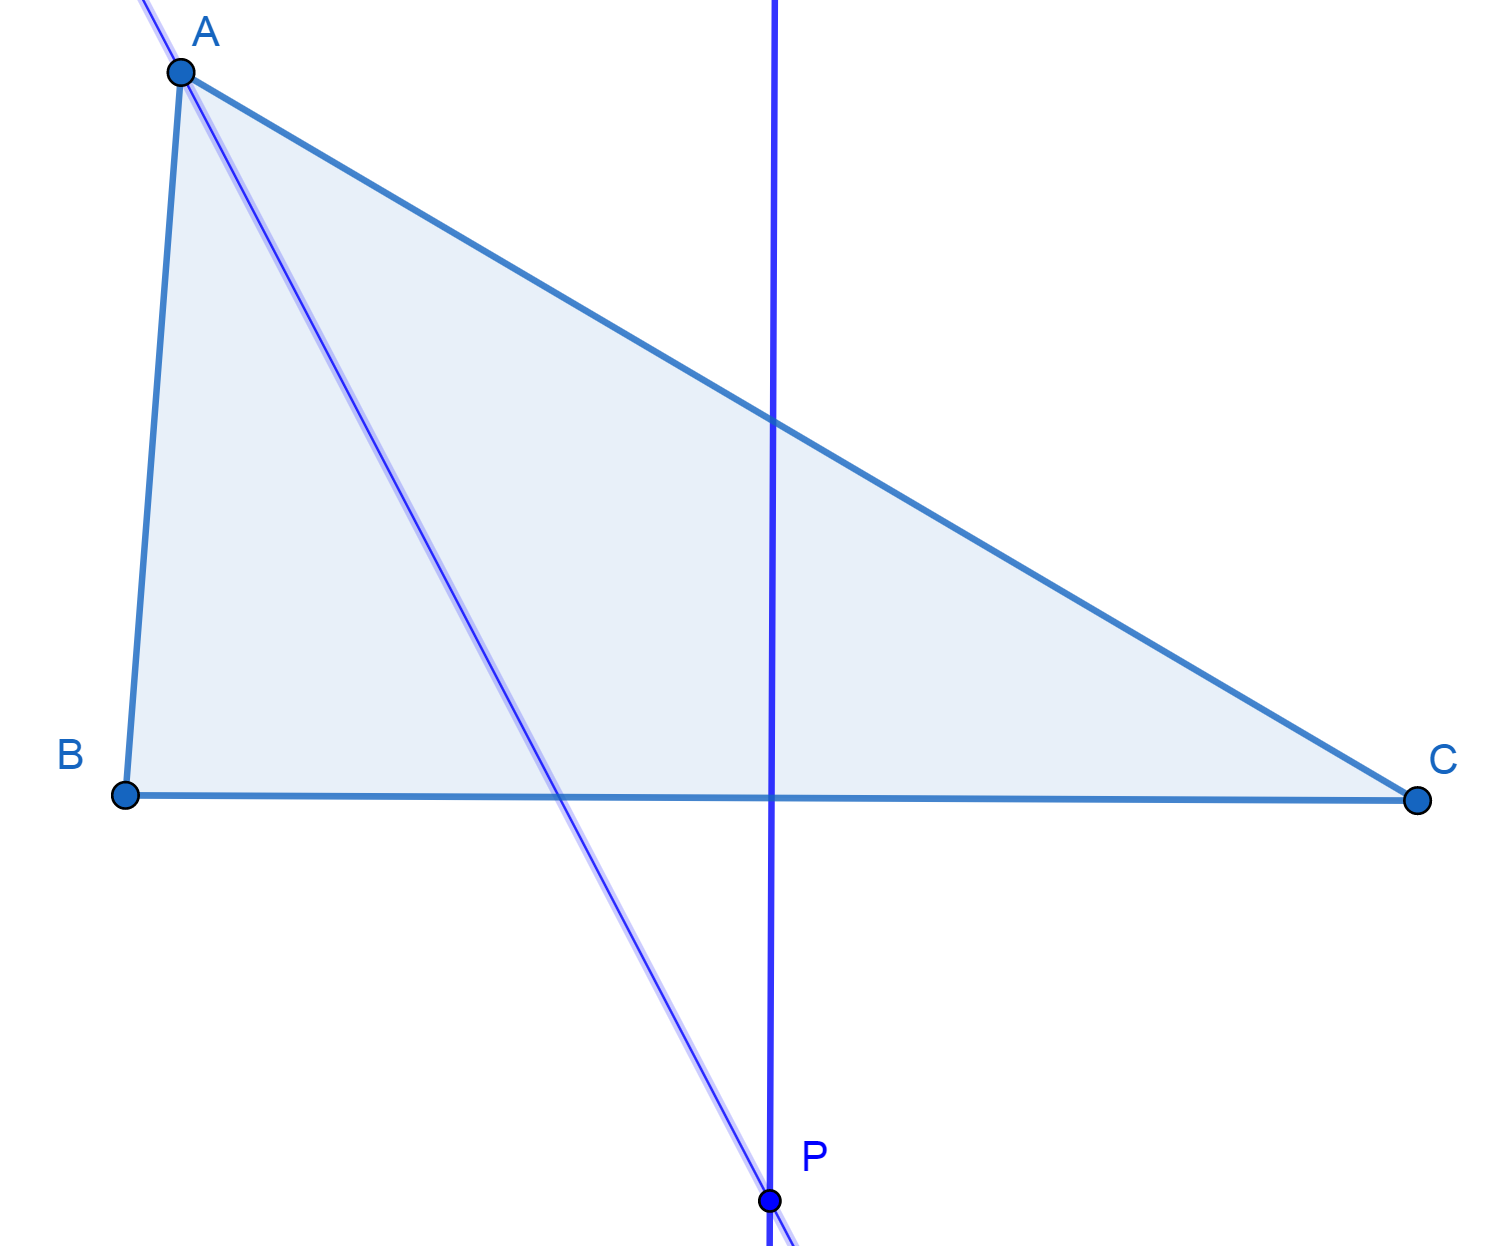
\includegraphics[width=.5\textwidth]{isoceles}
\end{center}


\tikzsetfigurename{geometry-theorems}
% !TeX root = bagrut-806.tex

\selectlanguage{hebrew}

%%%%%%%%%%%%%%%%%%%%%%%%%%%%%%%%%%%%%%%%%%%%%%%%%%%%%%%%%%%%%%%%%%%

\chapter{ייצוג גרפי של משפטים בגיאומטריה}\label{a.geometry}

%
% Thale's theorems
%
\selectlanguage{english}
\hspace*{-8mm}
\begin{minipage}[t]{.45\textwidth}
\begin{tikzpicture}[scale=1.2]
% Points of the triangle
\coordinate (a) at (0,0);
\coordinate (b) at (6,0);
\coordinate (c) at (4,3);
% Midpoints of the sides
\coordinate (mid1) at ($(a)!.5!(c)$);
\coordinate (mid2) at ($(b)!.5!(c)$);
% Draw the base and median
\draw[very thick,orange!80!black] (a) -- node[below] {$\bm{f}$} (b);
\draw[very thick,pink!60!black] (mid1) -- node[above] {$\bm{e}$} (mid2);
% Get the median
\coordinate (midbase) at ($(a)!.5!(b)$);
% Draw the triangle, sides in two parts
\draw[very thick,red] (a) -- node[above] {$\bm{b}$} (mid1);
\draw[very thick,blue] (mid1) -- node[above] {$\bm{a}$} (c);
\draw[very thick,green!60!black] (b) -- node[above,xshift=2pt] {$\bm{d}$} (mid2);
\draw[very thick,magenta] (mid2) -- node[above,xshift=2pt] {$\bm{c}$} (c);
% Dots at the midpoints
\fill (mid1) circle (2pt);
\fill (mid2) circle (2pt);
% Display first formula in color
\begin{scope}[xshift=2.5cm,yshift=.9cm]
\node[anchor=base,blue] at (0,0) {$\bm{a}$};
\node[anchor=base] at (.2,0) {$\bm{/}$};
\node[anchor=base,red] at (.4,0) {$\bm{b}$};
\node[anchor=base] at (.7,0) {$\bm{=}$};
\node[anchor=base,magenta] at (1,0) {$\bm{c}$};
\node[anchor=base] at (1.2,0) {$\bm{/}$};
\node[anchor=base,green!60!black] at (1.4,0) {$\bm{d}$};
\end{scope}
\begin{scope}[xshift=.9cm,yshift=.2cm]
% Display second formula in color
\node[anchor=base,blue] at (0,0) {$\bm{a}$};
\node[anchor=base] at (.2,0) {$\bm{/}$};
\node[anchor=base,blue] at (.5,0) {$\bm{(a}$};
\node[anchor=base] at (.9,0) {$\bm{+}$};
\node[anchor=base,red] at (1.3,0) {$\bm{b)}$};
\node[anchor=base] at (1.7,0) {$\bm{=}$};
\node[anchor=base,magenta] at (2.1,0) {$\bm{c}$};
\node[anchor=base] at (2.3,0) {$\bm{/}$};
\node[anchor=base,magenta] at (2.6,0) {$\bm{(c}$};
\node[anchor=base] at (3.0,0) {$\bm{+}$};
\node[anchor=base,green!60!black] at (3.4,0) {$\bm{d)}$};
\node[anchor=base] at (3.8,0) {$\bm{=}$};
\node[anchor=base,pink!60!black] at (4.1,0) {$\bm{e}$};
\node[anchor=base] at (4.3,0) {$\bm{/}$};
\node[anchor=base,orange!80!black] at (4.5,0) {$\bm{f}$};
\end{scope}
\end{tikzpicture}
\end{minipage}
\hspace{.1\textwidth}
\begin{minipage}[t]{.45\textwidth}
%
%  Angle bisector splits side proportionally
%
\begin{tikzpicture}[scale=1.2]
% Draw base and path two lines at known angles
\path[name path=ab] (0,0) coordinate (a) -- (0:6) coordinate (b);
\path[name path=ac] (a) -- node[left,xshift=-2pt,blue] {$\bm{a}$} +(60:4);
\path[name path=bc] (b) -- node[right,xshift=4pt,red] {$\bm{b}$} +(145:6);
% Get their intersection and draw lines to third vertex
\path[name intersections={of=ac and bc,by=c}];
\draw[blue,very thick] (a) -- (c);
\draw[red,very thick] (c) -- (b);
% Path bisectors of two lines
\path[name path=bisector] (c) -- +(-77.5:3.6);
% Intersection of angle bisectors
\draw[name intersections={of=bisector and ab,by=int}];
% Draw base of triangle
\draw[very thick,magenta] (a) -- node[below] {$\bm{c}$} (int);
\draw[very thick,green!60!black] (int) -- node[below] {$\bm{d}$} (b);
% Draw bisector and label angle
\draw[very thick] (c) -- (int);
\node[magenta,below,xshift=-3pt,yshift=-12pt] at (c) {$\bm{\alpha}$};
\node[magenta,below,xshift=11pt,yshift=-12pt] at (c) {$\bm{\alpha}$};
 Draw dot
\fill (int) circle (2pt);
% Display formula in color
\begin{scope}[xshift=29mm,yshift=4mm]
\node[anchor=base,blue] at (0,0) {$\bm{a}$};
\node[anchor=base] at (.2,0) {$\bm{/}$};
\node[anchor=base,red] at (.4,0) {$\bm{b}$};
\node[anchor=base] at (.7,0) {$\bm{=}$};
\node[anchor=base,magenta] at (1,0) {$\bm{c}$};
\node[anchor=base] at (1.2,0) {$\bm{/}$};
\node[anchor=base,green!60!black] at (1.4,0) {$\bm{d}$};
\end{scope}
\end{tikzpicture}
\end{minipage}

\bigskip\bigskip\bigskip

%%%%%%%%%%%%%%%%%%%%%%%%%%%%%%

%
% Medians of a triangle meet at a point with ratio 1:2
%
\selectlanguage{english}
\hspace*{-8mm}
\begin{minipage}[t]{.45\textwidth}
\begin{tikzpicture}[scale=1.2]
\coordinate (a) at (0,0);   % Points of the triangle
\coordinate (b) at (6,0);
\coordinate (c) at (4,3);
% Coordinates of bisectors
\coordinate (ab) at ($(a)!.5!(b)$);
\coordinate (bc) at ($(b)!.5!(c)$);
\coordinate (ac) at ($(a)!.5!(c)$);
% Draw the triangle and bisectors
\draw[blue,very thick] (a) -- node[above] {$\bm{x}$} (ac) -- node[above] {$\bm{x}$} (c);
\draw[red,very thick] (b) -- node[right] {$\bm{y}$} (bc) -- node[right] {$\bm{y}$} (c);
\draw[green!60!black,very thick] (a) -- node[below] {$\bm{z}$} (ab) -- node[below] {$\bm{z}$} (b);
\draw[very thick,red,name path=da] (a) -- (bc);
\draw[very thick,blue,name path=db] (b) -- (ac);
\draw[very thick,green!60!black,name path=dc] (c) -- (ab);
% Get their intersection
\path [name intersections={of=da and db,by={intersection}}];
% Labels
\path (a) -- node[above,red] {$\bm{2a}$} (intersection);
\path (bc) -- node[above,red] {$\bm{a}$} (intersection);
\path (b) -- node[above,blue] {$\bm{2b}$} (intersection);
\path (ac) -- node[above,blue] {$\bm{b}$} (intersection);
\path (c) -- node[right,green!60!black] {$\bm{2c}$} (intersection);
\path (ab) -- node[right,green!60!black] {$\bm{c}$} (intersection);
% Points at the intersections
\fill (intersection) circle (2pt);
\fill (ab) circle (2pt);
\fill (ac) circle (2pt);
\fill (bc) circle (2pt);
\end{tikzpicture}
\end{minipage}
\hspace{.1\textwidth}
%
% Bisector of hypothenuse is half the hypothenuse
%
\selectlanguage{english}
\begin{minipage}[t]{.45\textwidth}
\begin{tikzpicture}[scale=1.2]
\coordinate (a) at (0,0);   % Points of the triangle
\coordinate (b) at (6,0);
\coordinate (c) at (0,3);
% Dummy to raise figure
\path (2,-11pt) -- +(3,0);
% Coordinate of bisector
\coordinate (hyp) at ($(b)!.5!(c)$);
% Draw the triangle and bisectors
\draw[very thick] (b) -- (a) -- (c);
\draw[very thick,blue] (a) -- node[above,red] {$\bm{a}$} (hyp);
\draw[very thick,blue] (b) -- node[above,red] {$\bm{a}$} (hyp);
\draw[very thick,blue] (c) -- node[above,red] {$\bm{a}$} (hyp);
% Draw square to denote right angle
\draw (a) rectangle +(8pt,8pt);
% Points at the intersections
\fill (hyp) circle (2pt);
\end{tikzpicture}
\end{minipage}

\bigskip\bigskip\bigskip

%
% Inscribed circle center at meeting of angle bisectors
%
\selectlanguage{english}
\begin{minipage}[t]{.45\textwidth}
\begin{tikzpicture}[baseline=-6mm,scale=1.3]
% Draw base and path two lines at known angles
\draw[very thick] (0,0) coordinate (a) -- (0:5) coordinate (b);
\path[name path=ac] (a) -- +(60:3.5);
\path[name path=bc] (b) -- +(140:4.5);
% Get their intersection and draw lines to third vertex
\path[name intersections={of=ac and bc,by=c}];
\draw[very thick] (a) -- (c) -- (b);
% Path bisectors of two lines
\path[name path=bia,blue] (a) -- +(30:3.6);
\path[name path=bib,red] (b) -- +(160:5);
% Intersection of angle bisectors
\path [name intersections={of=bia and bib,by=center}];
%% Draw angle bisectors to center
\draw[very thick,red] (a) -- (center);
\draw[very thick,blue] (c) -- (center);
\draw[very thick,green!60!black] (b) -- (center);
%% Labels of angles
\node[red,right,xshift=14pt,yshift=4pt] at (a) {$\bm{\alpha}$};
\node[red,right,xshift=12pt,yshift=18pt] at (a) {$\bm{\alpha}$};
\node[blue,below,xshift=-4pt,yshift=-10pt] at (c) {$\bm{\beta}$};
\node[blue,below,xshift=10pt,yshift=-8pt] at (c) {$\bm{\beta}$};
\node[green!60!black,left,xshift=-30pt,yshift=6pt] at (b) {$\bm{\gamma}$};
\node[green!60!black,left,xshift=-30pt,yshift=20pt] at (b) {$\bm{\gamma}$};
%% Get perpendicular from center to one side and draw circle
\coordinate (perp) at ($(a)!(center)!(b)$);
\node [very thick,draw,circle through=(perp)] at (center) {};
%% Draw dot at center
\fill (center) circle (1.5pt);
\end{tikzpicture}
\end{minipage}
\hspace{.1\textwidth}
%
% Perpendicular bisectors meet in the center of the circumscribed circle
%
\selectlanguage{english}
\begin{minipage}[t]{.45\textwidth}
\begin{tikzpicture}[scale=.8]
% Circle goes from (a) to (b)
\coordinate (a) at (0,0);
\coordinate (b) at (6,0);
% Line containing lower points is (c) -- (d)
\coordinate (c) at (0,-2);
\coordinate (d) at (6,-2);
% Line containing upper points is (e) -- (f)
\coordinate (e) at (0,2);
\coordinate (f) at (4,3);
% Name the two chords
\path [name path=chord1] (c) -- (d);
\path [name path=chord2] (e) -- (f);
% Name the coordinate of the center of the circle
\coordinate (center) at ($ (a)!.5!(b) $);
% Draw a circle whose center is half-way between (a) and (b) through (a)
\node [draw,very thick,circle through=(a),name path=circ] at (center) {};
% Get intersections of the upper and lower lines with the circle
\path [name intersections={of=circ and chord1,by={i1,i2}}];
\path [name intersections={of=circ and chord2,by={i3,i4}}];
% Draw triangle
\draw [very thick,blue] (i1) -- node[left] {$\bm{a}$} ($(i1)!.5!(i3)$) --
  node[left] {$\bm{a}$} (i3);
\draw[very thick,green!60!black] (i3) -- node[right] {$\bm{b}$} ($(i3)!.5!(i2)$) --
  node[right] {$\bm{b}$} (i2);
\draw[very thick,red] (i2) -- node[below] {$\bm{c}$} ($(i2)!.5!(i1)$) -- 
  node[below] {$\bm{c}$} (i1);
% Draw three perpendicular bisectors
\draw [very thick,red,fill] (center) -- ($(i1)!(center)!(i2)$)
  circle[radius=1pt];
\draw [very thick,blue,fill] (center) -- ($(i1)!(center)!(i3)$)
  circle[radius=1pt];
\draw [very thick,green!60!black,fill] (center) -- ($(i2)!(center)!(i3)$)
  circle[radius=1pt];
% Draw squares to denote right angles
\draw[red] ($ (i1) !.5! (i2) $) rectangle +(6pt,6pt);
\draw[blue,rotate=-30] ($ (i1) !.5! (i3) $) rectangle +(6pt,6pt);
\draw[magenta,rotate=-160] ($ (i3) !.5! (i2) $)
  rectangle +(6pt,6pt);
% Draw dots at all intersections
\fill (i1) circle (3pt);
\fill (i2) circle (3pt);
\fill (i3) circle (3pt);
\fill (center) circle (3pt);
\end{tikzpicture}
\end{minipage}

\bigskip\bigskip

%
% Angles of tangent and angle subtending a chord are equal
%
\selectlanguage{english}
\hspace{8mm}
\begin{minipage}[t]{.45\textwidth}
\begin{tikzpicture}[scale=.7,baseline=-60pt]
% Circle goes from (a) to (b)
\coordinate (a) at (0,0);
\coordinate (b) at (6,0);
% Line containing lower point (d)
\coordinate (d) at (7,-2);
% Point outside circle is (e)
\coordinate (e) at (1.6,4);
% Name the lower chord
\path [name path=chord] (a) -- (d);
% Draw a circle whose center is half-way between (a) and (b) through (a)
\node [draw,very thick,circle through=(a),name path=circ] (circle) at ($ (a)!.5!(b) $) {};
% Get intersection of the lower line with the circle
\path [name intersections={of=circ and chord,by={i1,i2}}];
% Draw the tangent line
\coordinate (tan) at (tangent cs:node=circle, point={(e)}, solution=2);
\draw[very thick,blue] (e) -- ($ (e)!2!(tan) $);
% Draw the triangle
\draw [very thick,blue] (tan) node[below right,xshift=6pt,yshift=-10pt] {$\bm{\alpha}$} -- (i2);
\draw [very thick,red] (tan) -- (a) node[right,xshift=8pt,yshift=2pt] {$\bm{\alpha}$} -- (i2);
% Dots at intersections
\fill (a) circle (4pt);
\fill (i2) circle (4pt);
\fill (tan) circle(4pt);
\end{tikzpicture}
\end{minipage}
\hspace{.05\textwidth}
%
% Inscribed angle one half of central angle
%
\begin{minipage}[t]{.45\textwidth}
\hspace{3em}
\begin{tikzpicture}[scale=.7]
% Circle goes from (a) to (b)
\coordinate (a) at (0,0);
\coordinate (b) at (6,0);
\coordinate (center) at (3,0);
% Line containing lower points is (c) -- (d)
\coordinate (c) at (0,-2);
\coordinate (d) at (6,-2);
% Line containing upper points is (e) -- (f);
\coordinate (e) at (0,2.3);
\coordinate (f) at (4.5,3);
% Name the upper and lower lines
\path [name path=chord1] (c) -- (d);
\path [name path=chord2] (e) -- (f);
% Draw a circle whose center is half-way between (a) and (b) through (a)
\node [draw,very thick,circle through=(a),name path=circ] at (center) {};
% Get intersections of the upper and lower lines with the circle
\path [name intersections={of=circ and chord1,by={i1,i2}}];
\path [name intersections={of=circ and chord2,by={i3,i4}}];
% Draw the lower chord
%\draw[very thick] (i1) -- (i2);
% Draw the two subtended angles and the center angle
\draw[very thick,red] (i1) -- (i3)
  node[below,xshift=-3pt,yshift=-12pt] {$\bm{\alpha}$} -- (i2);
\draw[very thick,green!60!black] (i1) -- (i4)
  node[below,xshift=6pt,yshift=-12pt] {$\bm{\alpha}$} -- (i2);
\draw[very thick,blue] (i1) -- (center)
  node[below,yshift=-8pt] {$\bm{2\alpha}$} -- (i2);
% Dots at intersections
\fill (i1) circle (3pt);
\fill (i2) circle (3pt);
\fill (i3) circle (3pt);
\fill (i4) circle (3pt);
\fill (center) circle (3pt);
\end{tikzpicture}
\end{minipage}

\np

%
% Intersecting chords
%
\selectlanguage{english}
\begin{minipage}[t]{.45\textwidth}
\begin{tikzpicture}[scale=.7]
% Circle goes from (a) to (b)
\coordinate (a) at (0,0);
\coordinate (b) at (6,0);
% Line containing lower points is (c) -- (d)
\coordinate (c) at (0,-2);
\coordinate (d) at (6,-1.5);
% Line containing upper points is (e) -- (f)
\coordinate (e) at (0,1.5);
\coordinate (f) at (6,4);
% Name the upper and lower lines
\path [name path=chord1] (c) -- (d);
\path [name path=chord2] (e) -- (f);
% Draw a circle whose center is half-way between (a) and (b) through (a)
\node [draw,very thick,circle through=(a),name path=circ] at ($ (a)!.5!(b) $) {};
% Get intersections of the upper and lower lines with the circle
\path [name intersections={of=circ and chord1,by={i1,i2}}];
\path [name intersections={of=circ and chord2,by={i3,i4}}];
% Name the two chords
\path [name path=x1] (i1) -- (i3);
\path [name path=x2] (i2) -- (i4);
% Get their intersection
\path [name intersections={of=x1 and x2,by={p}}];
% Draw four lines from intersection to circle
\draw[very thick,red] (i1) -- node[left] {$\bm{a}$} (p);
\draw[very thick,blue] (p) --  node[left] {$\bm{b}$} (i3);
\draw[very thick,magenta] (i2) -- node[right,yshift=4pt] {$\bm{c}$} (p);
\draw[very thick,green!60!black] (p) -- node[right,yshift=4pt] {$\bm{d}$} (i4);
% Dots at intersections
\fill (p) circle (3pt);
\fill (i1) circle (3pt);
\fill (i2) circle (3pt);
\fill (i3) circle (3pt);
\fill (i4) circle (3pt);
% Display formula in color
\begin{scope}[xshift=2.3cm,yshift=-1.5cm]
\node[anchor=base,red] at (0,0) {$\bm{a}$};
\node[anchor=base,blue] at (10pt,0) {$\bm{b}$};
\node[anchor=base] at (23pt,0) {$\bm{=}$};
\node[anchor=base,magenta] at (36pt,0) {$\bm{c}$};
\node[anchor=base,green!60!black] at (46pt,0) {$\bm{d}$};
\end{scope}
\end{tikzpicture}
\end{minipage}
\hspace{.05\textwidth}
%
% Intersecting secants
%
\selectlanguage{english}
\begin{minipage}[t]{.45\textwidth}
\begin{tikzpicture}[scale=.7]
% Circle goes from (a) to (b)
\coordinate (a) at (0,0);
\coordinate (b) at (6,0);
% Line containing lower points is (c) -- (d)
\coordinate (c) at (1,-3);
\coordinate (d) at (7,1.5);
% Point outside circle is (e)
\coordinate (e) at (-1,4);
% Name the lower chord
\path [name path=chord] (c) -- (d);
% Draw a circle whose center is half-way between (a) and (b) through (a)
\node [draw,very thick,circle through=(a),name path=circ] at ($ (a)!.5!(b) $) {};
% Get intersection of the lower line with the circle
\path [name intersections={of=circ and chord,by={i1,i2}}];
% Draw the full secants
\draw [name path=secant1,very thick,green!60!black] (i1) -- node[left,xshift=6pt,yshift=-13pt] {$\bm{c}$} (e);
\draw [name path=secant2,very thick,blue] (i2) -- node[right,xshift=2pt,yshift=-8pt] {$\bm{a}$} (e);
% Get intersections of the secants with the circle
\path [name intersections={of=circ and secant1,by={s11,s12}}];
\path [name intersections={of=circ and secant2,by={s21,s22}}];
% Draw offset lines from outside point with the intersections of the secants
\draw[very thick,red]
  let \p1 = (s21), \p2 = (e) in
    (\x2-5pt,\y2) -- node[left] {$\bm{b}$} (\x1-5pt,\y1);
\draw[very thick,magenta]
  let \p1 = (s12), \p2 = (e) in
    (\x2+5pt,\y2+3pt) -- node[right,xshift=4pt,yshift=2pt] {$\bm{d}$} (\x1+4pt,\y1+2pt);
% Dots at intersections
\fill (s11) circle (3pt);
\fill (s12) circle (3pt);
\fill (s21) circle (3pt);
\fill (s22) circle (3pt);
\fill (s12) circle (3pt);
\fill (e) circle (3pt);
% Display formula in color
\begin{scope}[xshift=2.4cm,yshift=-4mm]
\node[anchor=base,blue] at (0,0) {$\bm{a}$};
\node[anchor=base,red] at (11pt,0) {$\bm{b}$};
\node[anchor=base] at (25pt,0) {$\bm{=}$};
\node[anchor=base,green!60!black] at (39pt,0) {$\bm{c}$};
\node[anchor=base,magenta] at (51pt,0) {$\bm{d}$};
\end{scope}
\end{tikzpicture}
\end{minipage}


\bigskip\bigskip

%
% Intersecting tangent and secant
%
\selectlanguage{english}
\begin{minipage}[t]{.45\textwidth}
\begin{tikzpicture}[scale=.7]
% Circle goes from (a) to (b)
\coordinate (a) at (0,0);
\coordinate (b) at (6,0);
% Line containing lower points is (c) -- (d)
\coordinate (c) at (1,-3);
\coordinate (d) at (7,1.5);
% Point outside circle is (e)
\coordinate (e) at (-1,4);
% Name the lower chord
\path [name path=chord] (c) -- (d);
% Draw a circle whose center is half-way between (a) and (b) through (a)
\node [draw,very thick,circle through=(a),name path=circ] (circle) at ($ (a)!.5!(b) $) {};
% Get intersection of the lower line with the circle
\path [name intersections={of=circ and chord,by={i1,i2}}];
% Draw the full secant
\draw [name path=secant2,very thick,blue] (i2) -- node[right,yshift=-4pt] {$\bm{a}$} (e);
% Get intersection of the secant with the circle
\path [name intersections={of=circ and secant2,by={s21,s22}}];
% Draw offset line from outside point with the intersection of the secant
\draw[very thick,red]
  let \p1 = (s21), \p2 = (e) in
    (\x2-5pt,\y2) -- node[left] {$\bm{b}$} (\x1-5pt,\y1);
% Draw the tangent line
\coordinate (tan) at (tangent cs:node=circle, point={(e)}, solution=2);
\draw[very thick,green!60!black] (e) -- node[right,yshift=4pt] {$\bm{c}$} (tan);
% Dots at intersections
\fill (s21) circle (3pt);
\fill (s22) circle (3pt);
\fill (e) circle (3pt);
\fill (tan) circle(3pt);
% Display formula in color
\begin{scope}[xshift=2.5cm]
\node[anchor=base,green!60!black] at (0,0) {$\bm{c^2}$};
\node[anchor=base] at (.6,0) {$\bm{=}$};
\node[anchor=base,blue] at (1.1,0) {$\bm{a}$};
\node[anchor=base,red] at (1.5,0) {$\bm{b}$};
\end{scope}
\end{tikzpicture}
\end{minipage}
\hspace{.05\textwidth}
%
% Intersecting tangents
%
\begin{minipage}[t]{.45\textwidth}
\begin{tikzpicture}[scale=.7]
% Circle goes from (a) to (b)
\coordinate (a) at (0,0);
\coordinate (b) at (6,0);
\coordinate (center) at (3,0);
% Point outside circle is (e)
\coordinate (e) at (-2,2);
\node [draw,very thick,circle through=(a),name path=circ] (circle) at (center) {};
% Draw the tangent line
\coordinate (tan1) at (tangent cs:node=circle, point={(e)}, solution=1);
\coordinate (tan2) at (tangent cs:node=circle, point={(e)}, solution=2);
\draw[very thick,blue] (e) -- node[left] {$\bm{a}$} (tan1);
\draw[very thick,red] (e) -- node[above] {$\bm{a}$} (tan2);
% Draw radii
\draw[ultra thick,dashed,green!60!black] (center) -- node[below] {$\bm{r}$} (tan1);
\draw[ultra thick,dashed,green!60!black] (center) -- node[right] {$\bm{r}$} (tan2);
% Draw right angles
\draw[very thick,green!60!black,rotate=34] (tan1) rectangle +(10pt,10pt);
\draw[very thick,green!60!black,rotate=-168] (tan2) rectangle +(10pt,10pt);
% Dots at intersections
\fill (e) circle (3pt);
\fill (center) circle (3pt);
\fill (tan1) circle(3pt);
\fill (tan2) circle(3pt);
\end{tikzpicture}
\end{minipage}


%%%%%%%%%%%%%%%%%%%%%%%%%%%%%%%%%%%%%%%%%%%%%%%%%%%%%%%%%%

\bigskip
\bigskip
\bigskip

%
% Sums of opposite sides of circumscribed quadrilateral are equal
%
\selectlanguage{english}
\begin{minipage}[t]{.45\textwidth}
\begin{tikzpicture}[scale=.65]
% Circle goes from (a) to (b)
\coordinate (x) at (0,3);
\coordinate (y) at (6,3);
\coordinate (a) at (-2,5.5);
% Draw a circle whose center is half-way between (a) and (b) through (a)
\node [draw,very thick,circle through=(x),name path=circ] (circle) at ($ (x)!.5!(y) $) {};
% Draw tangent lines
\coordinate (tan1) at (tangent cs:node=circle, point={(a)}, solution=1);
\draw[very thick,red] (a) -- node[below,xshift=-2pt] {$\bm{b}$}
  ($(a)!1.5!(tan1)$) coordinate (b);
\coordinate (tan2) at (tangent cs:node=circle, point={(a)}, solution=2);
\draw[very thick,magenta] (a) -- node[above] {$\bm{c}$}
  ($(a)!1.8!(tan2)$) coordinate (c);
\coordinate (tan3) at (tangent cs:node=circle, point={(c)}, solution=2);
\draw[very thick,blue] (c) -- node[right] {$\bm{a}$}
  ($(c)!1.51!(tan3)$)  coordinate (d);
\draw[very thick,green!60!black] (b) -- node[below] {$\bm{d}$} (d);
% Display formula in color
\begin{scope}[xshift=2cm,yshift=3cm]
\node[anchor=base,blue] at (0,0) {$\bm{a}$};
\node[anchor=base] at (.4,0) {$\bm{+}$};
\node[anchor=base,red] at (.8,0) {$\bm{b}$};
\node[anchor=base] at (1.3,0) {$\bm{=}$};
\node[anchor=base,magenta] at (1.8,0) {$\bm{c}$};
\node[anchor=base] at (2.2,0) {$\bm{+}$};
\node[anchor=base,green!60!black] at (2.6,0) {$\bm{d}$};
\end{scope}
\end{tikzpicture}
\end{minipage}
\hspace{.1\textwidth}
%
% Opposite angles in an inscribed quadrilateral add up to 180
%
\selectlanguage{english}
\begin{minipage}[t]{.45\textwidth}
\begin{tikzpicture}[scale=.75]
% Circle goes from (a) to (b)
\coordinate (a) at (0,0);
\coordinate (b) at (6,0);
% Line containing lower points is (c) -- (d)
\coordinate (c) at (0,-2);
\coordinate (d) at (6,-1.5);
% Line containing upper points is (e) -- (f)
\coordinate (e) at (0,1.5);
\coordinate (f) at (6,3);
% Name the upper and lower lines
\path [name path=chord1] (c) -- (d);
\path [name path=chord2] (e) -- (f);
% Draw a circle whose center is half-way between (a) and (b) through (a)
\node [draw,very thick,circle through=(a),name path=circ] at ($ (a)!.5!(b) $) {};
% Get intersections of the upper and lower lines with the circle
\path [name intersections={of=circ and chord1,by={i1,i2}}];
\path [name intersections={of=circ and chord2,by={i3,i4}}];
% Draw the two subtended angles
\draw[very thick,red] (i1) -- (i2)
  node[left,xshift=-3pt,yshift=6pt] {$\bm{180-\alpha}$} -- (i3);
\draw[very thick,blue] (i1) -- (i4)
  node[right,xshift=3pt,yshift=-8pt] {$\bm{\alpha}$} -- (i3);
% Dots at intersections
\fill (i1) circle (3pt);
\fill (i2) circle (3pt);
\fill (i3) circle (3pt);
\fill (i4) circle (3pt);
\end{tikzpicture}
\end{minipage}

\bigskip\bigskip\bigskip\bigskip

%
% Diagonals of parallelogram bisect each other
%
\begin{minipage}[t]{.45\textwidth}
\begin{tikzpicture}[scale=.8]
% Bottom side of parallelogram
\coordinate (a) at (0,0);
\coordinate (b) at (6,0);
% Draw parallelogram at angle 50
\draw[very thick,magenta] (a) -- node[left,xshift=-2pt,yshift=2pt] {$\bm{d}$} +(50:4) coordinate (c);
\draw[very thick,green!60!black] (c) -- node[above] {$\bm{c}$} +(6,0) coordinate (d);
\draw[very thick,magenta] (d) -- node[right] {$\bm{d}$} +(230:4) coordinate (b);
\draw[very thick,green!60!black] (b) -- node[below] {$\bm{c}$} (a);
% Name the two diagonals
\path [name path=d1] (a) -- (d);
\path [name path=d2] (b) -- (c);
% Get their intersection
\path [name intersections={of=d1 and d2,by={intersection}}];
% Draw diagonals
\draw[very thick,red] (a) -- node[above] {$\bm{a}$} (intersection);
\draw[very thick,red] (intersection) -- node[above] {$\bm{a}$} (d);
\draw[very thick,blue] (b) -- node[above] {$\bm{b}$} (intersection);
\draw[very thick,blue] (intersection) -- node[above] {$\bm{b}$} (c);
% Dot at their intersection
\fill (intersection) circle (3pt);
\end{tikzpicture}
\end{minipage}
\hspace{.1\textwidth}
%
% Median of a trapezoid is average of sides
%
\selectlanguage{english}
\begin{minipage}[t]{.45\textwidth}
\begin{tikzpicture}
% Bottom of trapeze
\coordinate (a) at (0,0);
\coordinate (b) at (6,0);
% Draw the bases of the trapeze
\draw[very thick,magenta] (a) -- node[below] {$\bm{d}$} (b);
\path (a) -- ++(60:3) coordinate (c) -- ++(1.8,0) coordinate (d);
\draw[very thick,orange!80!black] (c) -- node[above] {$\bm{c}$} (d);
% Draw the sides of the trapeze in two parts
\coordinate (mid1) at ($(a)!.5!(c)$);
\coordinate (mid2) at ($(b)!.5!(d)$);
\draw[very thick,red] (a) -- node[left,xshift=-2pt] {$\bm{a}$} (mid1);
\draw[very thick,red] (mid1) -- node[left,xshift=-2pt] {$\bm{a}$} (c);
\draw[very thick,blue] (b) -- node[right,xshift=2pt] {$\bm{b}$} (mid2);
\draw[very thick,blue] (mid2) -- node[right,xshift=2pt] {$\bm{b}$} (d);
% Draw the median
\draw[very thick,green!60!black] (mid1) -- (mid2);
% Display formula in color
\begin{scope}[xshift=17mm,yshift=15mm]
\node[anchor=base] at (0,0) {$\bm{(}$};
\node[anchor=base,orange!80!black] at (.2,0) {$\bm{c}$};
\node[anchor=base] at (.5,0) {$\bm{+}$};
\node[anchor=base,magenta] at (.8,0) {$\bm{d}$};
\node[anchor=base] at (1.0,0) {$\bm{)}$};
\node[anchor=base] at (1.2,0) {$\bm{/}$};
\node[anchor=base] at (1.4,0) {$\bm{2}$};
\end{scope}
% Dots at the midpoints
\fill (mid1) circle (2pt);
\fill (mid2) circle (2pt);
\end{tikzpicture}
\end{minipage}

\selectlanguage{english}

\tikzsetfigurename{unit-circle}
% !TeX root = chapter-4-5.tex

\np

\selectlanguage{hebrew}

\chapter{מעגל היחידה}\label{a.unit-circle}

\section{רביעים של מעגל היחידה}

מעגל שהרדיוס שלו 
$1$
נקרא
\textbf{מעגל היחידה}.

\vspace{-2ex}

\begin{center}
\selectlanguage{english}
% The unit circle
\begin{tikzpicture}[scale=1.8]
\coordinate (origin) at (0,0);
% Draw circle
\draw[name path=circle] (origin) node [above left] {$(0,0)$} circle [radius=1];
% Draw axes
\draw[name path=x] (-1,0) node [left] {$(-1,0)$} -- (1,0) node [right] {$(1,0)$};
\draw (0,-1) node [below] {$(0,-1)$} -- (0,1) node [above] {$(0,1)$};
% Draw ray
\draw[rotate=30,name path=ray] (origin) node [above right,xshift=8mm] {$\theta$} -- node [above] {$1$} (1,0);
% Get intersection of circle and ray
\path [name intersections={of=circle and ray, by=on-circle}];
% Draw altitude from intersection to x-axis
\draw[name path=altitude] (on-circle) node[above right] {$(\cos\theta,\sin\theta)$} -- node [right,xshift=4mm] {$\sin \theta$} (on-circle |- origin);
\draw[->] (1.1,.25) -- +(-6pt,0);
% Get intersection of altitude and x-axis
\path [name intersections={of=altitude and x, by=on-x}] (origin) -- node [below] {$\cos \theta$} (on-x);
% Square for right angle at intersection
\draw (on-x) rectangle +(-2pt,2pt);
% Dot at origin
\fill (origin) circle [radius=1pt];
\end{tikzpicture}
\end{center}

\vspace{-3ex}

הצירים את מעגל היחידה באופן טבעי לארבעה
\textbf{רבעים}.
זוויות נמדדות 
\textbf{מעלות}
בין
$0^\circ$
ל-%
$360^\circ$,
כאשר הכיוון החיובי הוא נגד כיוון השעון. 
יחידה אחרת לזווית היא ה-%
\textbf{רדיאן}.
רדיאן אחד הוא הזווית כולאת קשת על היקף המעגל שאורכו שווה לרדיוס. במעגל היחידה הרדיוס הוא
$1$
ולכן אורך ההיקף הוא
$2\pi$.
כאשר קרן מסתובבת לאורך כל ההיקף )נגד כיוון השעון( היא עוברת מזווית
$0$
רדיאנים לזווית
$2\pi$
רדיאנים. רדיאן אחד שווה בערך
$57.3$	
מעלות.
\begin{center}
\selectlanguage{english}
% The unit circle with main axes
\begin{tikzpicture}[scale=1.8]
\coordinate (origin) at (0,0);
% Draw circle
\draw (origin) circle [radius=1];
% Draw axes
\draw (-1,0) node [left] {$180,-180$} -- (1,0) node [right] {$0,\pm 360$};
\draw (0,-1) node [below] {$270,-90$} -- (0,1) node [above] {$90,-270$};
% Dot at origin
\fill (origin) circle [radius=1pt];
\end{tikzpicture}
\hspace{3em}
\begin{tikzpicture}[scale=1.8]
\coordinate (origin) at (0,0);
% Draw circle
\draw (origin) circle [radius=1];
% Draw axes
\draw (-1,0) node [left] {$\pi,-\pi$} -- (1,0) node [right] {$0,\pm 2\pi$};
\draw (0,-1) node [below] {$3\pi/2,-\pi/2$} -- (0,1) node [above] {$\pi/2,-3\pi/2$};
% Draw one radian
\draw[thick] (origin) -- (57.3:1);
\draw[thick]  (1,0) arc(0:57:1);
\node at (29:1.15) {$1$};
% Dot at origin
\fill (origin) circle [radius=1pt];
\end{tikzpicture}
\end{center}

מהחיתוכים של הצירים עם מעגל היחידה נקבל את ערכי הסינוס והקוסינוס של הזוויות:
\begin{displaymath}
\renewcommand{\arraystretch}{.7}
\begin{array}{|c|c|c|c|}
\hline
\textrm{\R{זווית}} & \textrm{\R{זווית}} & \sin & \cos\\
\textrm{(\R{מעלות})} & \textrm{(\R{רדיאנים})} & & \\\hline
0 & 0 & 0 & 1\\\hline
90 & \pi/2 & 1 & 0\\\hline
180 & \pi & 0 & -1\\\hline
270 & 3\pi/2 & -1 & 0\\
\hline
\end{array}
\end{displaymath}

\np

%%%%%%%%%%%%%%%%%%%%%%%%%%%%%%%%%%%%%%%%%%%%%%%%%%%%%%%%%%%%%%%


\section{חלוקת מעגל היחידה ל
$8$
קטעים
}

תחילה נחלק כל רביע בחצי ונקבל
$8$
קטעים. הזווית של כל קטע הוא
$45^\circ$
או
$\pi/4$
רדיאנים:
\begin{center}
\selectlanguage{english}
% The unit circle divided into 45 degree segments
\begin{tikzpicture}[scale=1.8]
\coordinate (origin) at (0,0);
% Draw circle
\draw (origin) circle [radius=1];
% Draw axes
\draw (-1,0) node [left] {$180$} -- (1,0) node [right] {$0$};
\draw (0,-1) node [below] {$270$} -- (0,1) node [above] {$90$};
% Draw other angles
\draw[dashed] (origin) -- +(45:1) node[above right] {$45$};
\draw[dashed] (origin) -- +(135:1) node[above left] {$135$};
\draw[dashed] (origin) -- +(225:1) node[below left] {$225$};
\draw[dashed] (origin) -- +(315:1) node[below right] {$315$};
% Dot at origin
\fill (origin) circle [radius=1pt];
\end{tikzpicture}
\hspace{5em}
% The unit circle with radians divided into pi/4 segments
\begin{tikzpicture}[scale=1.8]
\coordinate (origin) at (0,0);
% Draw circle
\draw (origin) circle [radius=1];
% Draw axes
\draw (-1,0) node [left] {$\pi$} -- (1,0) node [right] {$0$};
\draw (0,-1) node [below] {$3\pi/2$} -- (0,1) node [above] {$\pi/2$};
% Draw other angles
\draw[dashed] (origin) -- +(45:1) node[above right] {$\pi/4$};
\draw[dashed] (origin) -- +(135:1) node[above left] {$3\pi/4$};
\draw[dashed] (origin) -- +(225:1) node[below left] {$5\pi/4$};
\draw[dashed] (origin) -- +(315:1) node[below right] {$7\pi/4$};
% Dot at origin
\fill (origin) circle [radius=1pt];
\end{tikzpicture}
\end{center}


במשולש 
$\triangle ABC$
אם הזווית
$\angle BAC$
הוא
$45^\circ$,
הזווית הנגדית
$\angle ABC$
חייבת להיות גם היא
$45^\circ$
כדי שסכום הזוויות במשולש יהיה
$180^\circ$.
המשולש שווי-שוקיים כך שערכי הסינוס והקוסינוס שווים. 
\begin{center}
\selectlanguage{english}
% Right triangle with 45 degree angles
\begin{tikzpicture}[scale=3.5]
% Coordinates
\coordinate (origin) at (0,0);
\coordinate (lower-right) at (1,0);
\coordinate (upper-right) at (1,1);
% Draw triangle
\draw (origin) node[left] {$A$} node[above right,xshift=10pt] {$45$} -- node[below] {$\cos 45$} (lower-right) node[right] {$C$} -- node[right] {$\sin 45$} (upper-right) node[right] {$B$} node[below left,xshift=2pt,yshift=-10pt] {$45$} -- node[left,xshift=-2pt,yshift=2pt] {$1$} cycle;
% Square for right angle
\draw (lower-right) rectangle +(-2pt,2pt);
\end{tikzpicture}
\end{center}
ממשפט פיתגורס:
\erh{14pt}
\begin{equationarray*}{rcl}
\sin^2 45 + \cos^2 45 &=& 1\\
2\sin^2 45 &=& 1\\
\sin 45 &=& \frac{1}{\sqrt{2}} = \frac{1}{\sqrt{2}}\cdot \frac{2}{2} =\frac{\sqrt{2}}{2}\\
\cos 45 &=& \sin 45 = \frac{\sqrt{2}}{2}\,.
\end{equationarray*}

%%%%%%%%%%%%%%%%%%%%%%%%%%%%%%%%%%%%%%%%%%%%%%%%%%%%%%%%%%%%%%%

\section{סינוס וקוסינוס של זוויות הגדולות מ-%
$90^\circ$}

עכשיו שאנו יודעים את ערכי הסינוס והקוסינוס של
$45^\circ$,
נוכל לשאול על הזוויות הסימטריות
$135^\circ$, $225^\circ$, $315^\circ$.
בעזרת חברינו מעגל היחידה, נמצא מיד את ערכי הסינוס והקוסינוס שלהן.

תחילה נחשב את הערכים עבור זווית שרירותית
$\theta$
ברביע הראשון. היטלי הקרניים על הצירים
$x,y$
שווים כך שיש רק לשנות את הסימנים. ברביע השני:

\np

\begin{center}
\selectlanguage{english}
% Functions of 180-\theta
\begin{tikzpicture}[scale=2]
\coordinate (origin) at (0,0);
% Draw circle
\draw[name path=circle] (origin) circle [radius=1];
% Draw axes
\draw (-1,0) -- (1,0);
\draw (0,-1) -- (0,1);
% Draw first ray
\path[name path=ray1] (origin) -- +(40:1.1);
\path[name intersections={of=circle and ray1,by=on-circle1}];
\draw (origin) node[above right,xshift=14pt,yshift=-1pt] {$\theta$} -- (on-circle1) node[above right,xshift=-4pt] {$(\cos \theta, \sin \theta)$};
% Draw altitude and square for right angle
\draw[dashed] (on-circle1) -- (on-circle1 |- origin);
\draw (on-circle1 |- origin) rectangle +(-2pt,2pt);
% Draw second ray
\path[name path=ray2] (origin) -- +(140:1.1);
\path[name intersections={of=circle and ray2,by=on-circle2}];
\draw (origin) -- (on-circle2) node[above left,xshift=4pt] {$(-\cos \theta, \sin \theta)$};
% Draw altitude and square for right angle
\draw[dashed] (on-circle2) -- (on-circle2 |- origin);
\draw (on-circle2 |- origin) rectangle +(2pt,2pt);
% Draw the arc for 180-\theta
\draw (12pt,0) arc(0:140:12pt);
\node at (8pt,18pt) {$180-\theta$};
\draw[->] (6pt,16pt) -- +(0,-4pt);
\end{tikzpicture}
\end{center}

\vspace{-8ex}

\erh{12pt}
\begin{equationarray*}{rcl}
\cos 135&=&\cos (180-45)= -\cos 45= \displaystyle -\frac{\sqrt{2}}{2}\\
\sin 135&=&\sin (180-45)= \sin 45= \displaystyle \frac{\sqrt{2}}{2}\,.
\end{equationarray*}

\vspace{-4ex}

נסתכל על הרביע השלישי והרביע הרביעי:
\begin{center}
\selectlanguage{english}
% Functions of 180+\theta
\begin{tikzpicture}[scale=1.8]
\coordinate (origin) at (0,0);
% Draw circle
\draw[name path=circle] (origin) circle [radius=1];
% Draw axes
\draw (-1,0) -- (1,0);
\draw (0,-1) -- (0,1);
% Draw first ray
\path[name path=ray1] (origin) -- +(40:1.1);
\path[name intersections={of=circle and ray1,by=on-circle1}];
\draw (origin) node[above right,xshift=14pt,yshift=-1pt] {$\theta$} -- (on-circle1) node[above right,xshift=-4pt] {\shortstack{$(\cos \theta,$\\$\sin \theta)$}};
% Draw altitude and square for right angle
\draw[dashed] (on-circle1) -- (on-circle1 |- origin);
\draw (on-circle1 |- origin) rectangle +(-2pt,2pt);
% Draw second ray
\path[name path=ray2] (origin) -- +(-140:1.1);
\path[name intersections={of=circle and ray2,by=on-circle2}];
\draw (origin) -- (on-circle2) node[below left,xshift=4pt] {\shortstack{$(-\cos \theta,$\\$-\sin \theta)$}};
% Draw altitude and square for right angle
\draw[dashed] (on-circle2) -- (on-circle2 |- origin);
\draw (on-circle2 |- origin) rectangle +(2pt,-2pt);
% Draw the arc for 180+\theta
\draw (12pt,0) arc(0:220:12pt);
\node at (8pt,18pt) {$180+\theta$};
\draw[->] (6pt,16pt) -- +(0,-4pt);
\end{tikzpicture}
\hspace{3em}
% Functions of -\theta
\begin{tikzpicture}[scale=1.8,baseline=-66pt]
\coordinate (origin) at (0,0);
% Draw circle
\draw[name path=circle] (origin) circle [radius=1];
% Draw axes
\draw (-1,0) -- (1,0);
\draw (0,-1) -- (0,1);
% Draw first ray
\path[name path=ray1] (origin) -- +(40:1.1);
\path[name intersections={of=circle and ray1,by=on-circle1}];
\draw (origin) node[above right,xshift=12pt] {$\theta$} -- (on-circle1) node[right,xshift=4pt] {\shortstack{$(\cos \theta,$\\$\sin \theta)$}};
% Draw altitude and square for right angle
\draw[dashed] (on-circle1) -- (on-circle1 |- origin);
\draw (on-circle1 |- origin) rectangle +(-2pt,2pt);
% Draw second ray
\path[name path=ray2] (origin) -- +(-40:1.1);
\path[name intersections={of=circle and ray2,by=on-circle2}];
\draw (origin) node[below right,xshift=13pt] {$-\theta$} -- (on-circle2) node[right,xshift=4pt] {\shortstack{$(\cos \theta,$\\$-\sin \theta)$}};
% Draw altitude and square for right angle
\draw[dashed] (on-circle2) -- (on-circle2 |- origin);
\draw (on-circle2 |- origin) rectangle +(-2pt,-2pt);
\end{tikzpicture}
\end{center}


\vspace{-3ex}

עבור הרביע השליש:
\erh{14pt}
\begin{equationarray*}{rcl}
\cos 225 &=&\cos (180+45)= -\cos 45= \displaystyle -\frac{\sqrt{2}}{2}\\
\sin 225 &=&\sin (180+45)= -\sin 45= \displaystyle -\frac{\sqrt{2}}{2}\,.
\end{equationarray*}


\vspace{-2ex}

עבור הרבע הרביעי, נוח להשתמש בזווית השלילית
$-\theta$
במקום הזווית החיובית
$360-\theta$:
\erh{12pt}
\begin{equationarray*}{rcl}
\cos 315=\cos (-45)= \cos 45= \displaystyle \frac{\sqrt{2}}{2}\\
\sin 315=\sin (-45)= -\sin 45= \displaystyle -\frac{\sqrt{2}}{2}\,.
\end{equationarray*}

\np

נסכם את הערכים בטבלה:
\begin{displaymath}
\renewcommand{\arraystretch}{.7}
\begin{array}{|c|c|c|c|}
\hline
\textrm{\R{זווית}} & \textrm{\R{זווית}} & \sin & \cos\\
\textrm{(\R{מעלות})} & \textrm{(\R{רדיאנים})} & & \\\hline
\theta& \theta&  \sin\theta &  \cos\theta \\\hline
180-\theta& \pi - \theta&  \sin\theta &  -\cos\theta\\\hline
180+\theta& \pi+\theta&  -\sin\theta &  -\cos\theta\\\hline
-\theta& \theta&  -\sin\theta &  \cos\theta\\
\hline
\end{array}
\end{displaymath}


ועבור
$45^\circ$:
\begin{displaymath}
\renewcommand{\arraystretch}{.8}
\begin{array}{|c|c|c|c|}
\hline
\textrm{\R{זווית}} & \textrm{\R{זווית}} & \sin & \cos\\
\textrm{(\R{מעלות})} & \textrm{(\R{רדיאנים})} & & \\\hline
45& \pi/4&  \sqrt{2}/2 &  \sqrt{2}/2 \\\hline
135& 3\pi/4&  \sqrt{2}/2 &  -\sqrt{2}/2\\\hline
225& 5\pi/4&  -\sqrt{2}/2 &  -\sqrt{2}/2\\\hline
315& 7\pi/4&  -\sqrt{2}/2 &  \sqrt{2}/2\\
\hline
\end{array}
\end{displaymath}

%%%%%%%%%%%%%%%%%%%%%%%%%%%%%%%%%%%%%%%%%%%%%%%%%%%%%%%%%%%%%%%

\section{הסינוס והקוסינוס של
$30^\circ$
ו
$60^\circ$}

את מעגל היחידה ניתן לחלק ל-%
$6$
קטעים של
$60^\circ$
או ל-%
$12$
קטעים של
$30^\circ$:
\begin{center}
\selectlanguage{english}
% The unit circle divided into 60 degree segments
\begin{tikzpicture}[scale=1.8]
\coordinate (origin) at (0,0);
% Draw circle
\draw (origin) circle [radius=1];
% Draw axes
\draw (-1,0) node [left] {$180$} -- (1,0) node [right] {$0$};
%\draw (0,-1) node [below] {$270$} -- (0,1) node [above] {$90$};
% Draw other angles
\draw[dashed] (origin) -- +(60:1) node[above right] {$60$};
\draw[dashed] (origin) -- +(120:1) node[above left] {$120$};
\draw[dashed] (origin) -- +(240:1) node[below left] {$240$};
\draw[dashed] (origin) -- +(300:1) node[below right] {$300$};
% Dot at origin
\fill (origin) circle [radius=1pt];
\end{tikzpicture}
\hspace{5em}
% The unit circle divided into 30 degree segments
\begin{tikzpicture}[scale=1.8,baseline=-60pt]
\coordinate (origin) at (0,0);
% Draw circle
\draw (origin) circle [radius=1];
% Draw axes
\draw (-1,0) node [left] {$180$} -- (1,0) node [right] {$0$};
\draw (0,-1) node [below] {$270$} -- (0,1) node [above] {$90$};
% Draw other angles
\draw[dashed] (origin) -- +(30:1) node[above right] {$30$};
\draw[dashed] (origin) -- +(60:1) node[above right] {$60$};
\draw[dashed] (origin) -- +(120:1) node[above left] {$120$};
\draw[dashed] (origin) -- +(150:1) node[above left] {$150$};
\draw[dashed] (origin) -- +(210:1) node[below left] {$210$};
\draw[dashed] (origin) -- +(240:1) node[below left] {$240$};
\draw[dashed] (origin) -- +(300:1) node[below right] {$300$};
\draw[dashed] (origin) -- +(330:1) node[below right] {$330$};
% Dot at origin
\fill (origin) circle [radius=1pt];
\end{tikzpicture}
\end{center}

\np

ברדיאנים:
\begin{center}
\selectlanguage{english}
% The unit circle with radians divided into pi/3 segments
\begin{tikzpicture}[scale=1.8]
\coordinate (origin) at (0,0);
% Draw circle
\draw (origin) circle [radius=1];
% Draw axes
\draw (-1,0) node [left] {$\pi$} -- (1,0) node [right] {$0$};
% Draw other angles
\draw[dashed] (origin) -- +(60:1) node[above right] {$\pi/3$};
\draw[dashed] (origin) -- +(120:1) node[above left] {$2\pi/3$};
\draw[dashed] (origin) -- +(240:1) node[below left] {$4\pi/3$};
\draw[dashed] (origin) -- +(300:1) node[below right] {$5\pi/3$};
% Dot at origin
\fill (origin) circle [radius=1pt];
\end{tikzpicture}
\hspace{4em}
% The unit circle with radians divided into pi/6 segments
\begin{tikzpicture}[scale=1.8,baseline=-62pt]
\coordinate (origin) at (0,0);
% Draw circle
\draw (origin) circle [radius=1];
% Draw axes
\draw (-1,0) node [left] {$\pi$} -- (1,0) node [right] {$0$};
\draw (0,-1) node [below] {$3\pi/2$} -- (0,1) node [above] {$\pi/2$};
% Draw other angles
\draw[dashed] (origin) -- +(30:1) node[above right] {$\pi/6$};
\draw[dashed] (origin) -- +(60:1) node[above right] {$\pi/3$};
\draw[dashed] (origin) -- +(120:1) node[above left] {$2\pi/3$};
\draw[dashed] (origin) -- +(150:1) node[above left] {$5\pi/6$};
\draw[dashed] (origin) -- +(210:1) node[below left] {$7\pi/6$};
\draw[dashed] (origin) -- +(240:1) node[below left] {$4\pi/3$};
\draw[dashed] (origin) -- +(300:1) node[below right] {$5\pi/3$};
\draw[dashed] (origin) -- +(330:1) node[below right] {$11\pi/6$};
% Dot at origin
\fill (origin) circle [radius=1pt];
\end{tikzpicture}
\end{center}

נחשב תחילה את הסינוס של 
$30^\circ$.
במשולש ישר-זווית:
\begin{center}
\selectlanguage{english}
% Right triangle with 30 and 60 degree angles
\begin{tikzpicture}[scale=6]
% Coordinates
\coordinate (origin) at (0,0);
\coordinate (lower-right) at (1,0);
\coordinate (upper-right) at (1,.5);
% Draw triangle
\draw (origin)
  node[left] {$A$} node[above right,xshift=24pt] {$30$} --
  node[below] {$b=\cos 30$} (lower-right) node[right] {$C$} --
  node[right] {$a=\sin 30$} (upper-right)
    node[right] {$B$} node[below left,yshift=-5pt] {$60$} --
  node[left,yshift=5pt] {$1$} cycle;
% Square for right angle
\draw (lower-right) rectangle +(-1pt,1pt);
\end{tikzpicture}
\end{center}

צייר קו מ-%
$C$
אל היתר כך שהזווית עם הצלע
$AC$
היא 
$30^\circ$:
\begin{center}
\selectlanguage{english}
% Right triangle with 30 and 60 degree angles
\begin{tikzpicture}[scale=6]
% Coordinates
\coordinate (origin) at (0,0);
\coordinate (lower-right) at (1,0);
\coordinate (upper-right) at (1,.5);
% Draw triangle
\draw (origin)
  node[left] {$A$} node[above right,xshift=24pt] {$30$} --
  node[below] {$b=\cos 30$} (lower-right) node[right] {$C$} --
  node[right] {$a=\sin 30$} (upper-right)
  node[right] {$B$} node[below left,yshift=-5pt] {$60$} --
  cycle;
% Get intersection of hypotenuse with line at 30 degrees
\path[name path=hypotenuse] (origin) -- (upper-right);
\path[name path=to-hyp] (lower-right) -- +(150:6mm);
\path[name intersections={of=hypotenuse and to-hyp,by=on-hyp}];
% Draw the line and label the angles
\draw (lower-right) 
    node[above left,yshift=5pt,xshift=2pt] {$60$}
    node [left,yshift=6pt,xshift=-16pt] {$30$} --
    (on-hyp)
    node[right,xshift=8pt] {$60$}
    node[below,yshift=-4pt] {$120$}
    node[above] {$D$};
% Label line segments
\path (lower-right) -- node[above] {$a$} (on-hyp);
\path (on-hyp) -- node[above] {$a$} (upper-right);
\path (origin) -- node[above,yshift=4pt] {$1-a$} (on-hyp);
% Square for right angle
\draw (lower-right) rectangle +(-1pt,1pt);
\end{tikzpicture}
\end{center}
מעובדות על זוויות במשולש השלמנו בציור את שאר הזוויות. המשולש
$\triangle BCD$
שווי-צלעות ואורך כל צלע הוא
$a=\sin 30$.
בנוסף,
$\triangle ACD$
שווי-שוקיים כך ש-%
$a=1-a$
)זכור שהמשלוש נמצא במעגל היחידה ואורך היתר הוא
$1$(.
מכאן:
\[
\sin a = a = 1-a = \frac{1}{2}\,.
\]
מהנוסחה
$\sin^2\theta + \cos^2\theta = 1$
מתקבל ערך הקוסינוס:
\[
\cos 30 = \sqrt{1-\sin^2 30} = \sqrt{1-\left(\frac{1}{2}\right)^2} = \sqrt{\frac{3}{4}} = \frac{\sqrt{3}}{2}\,.
\]

%%%%%%%%%%%%%%%%%%%%%%%%%%%%%%%%%%%%%%%%%%%%%%%%%%%%%%%%%%%%%%%

\np

\section{סינוס וקוסינוס של
$(90-\theta)$}

נפנה עכשיו לחישוב של סינוס וקוסינוס של
$60^\circ$.
מ-
$60 = 90 - 30$,
את הקשר בין
$60^\circ$
ו-
$30^\circ$
ניתן לראות מהזוויות של
$90-\theta$
במעגל היחידה:
\begin{center}
\selectlanguage{english}
% Quadrant with angle 90 - theta
\begin{tikzpicture}[scale=3.5]
\coordinate (origin) at (0,0);
% Draw arc
\draw[name path=arc] (1,0) arc [start angle=0, end angle=90, radius=1];
% Draw x-axis
\draw[name path=x] (origin) -- (1,0);
% Draw y-axis
\draw (origin) -- (0,1);
% Draw ray
\draw[rotate=60,name path=ray] (origin) node [above right,xshift=2mm] {$90-\theta$} -- node [above,yshift=1pt,xshift=-1pt] {$1$} (1,0);
% Get intersection of arc and ray
\path [name intersections={of=ray and arc, by=on-circle}];
% Draw altitude from intersection to x-axis
\draw[name path=altitude] (on-circle) node[below,yshift=-8pt,xshift=-4pt] {$\theta$} -- node [right] {$\sin (90-\theta)$} (on-circle |- origin);
% Get intersection of altitude and x-axis
\path [name intersections={of=altitude and x, by=on-x}] (origin) -- node [below] {$\cos (90-\theta)$} (on-x);
% Square for right angle at intersection
\draw (on-x) rectangle +(-1pt,1pt);
% Dot at origin
\fill (origin) circle [radius=.5pt];
\end{tikzpicture}
\end{center}
הזווית בנקודה שהמשולש נושק למעגל היחידה היא
$\theta$,
כך שהפונקציות הטריגונומטריות של
$90-\theta$
מתקבלות מאלו של 
$\theta$
על ידי החלפת הצלעות "נגדי" ו-"צדדי" בהגדרות:
\begin{eqnarray*}
\cos (90-\theta) &=& \sin \theta\\
\sin (90-\theta) &=& \cos \theta\,.
\end{eqnarray*}
דרך אחרת לראות את הקשר היא לשים לב שהמשולש חופף את המשולש לחשב
$\sin\theta$
ו-
$\cos \theta$:

\vspace{-2ex}

\begin{center}
\selectlanguage{english}
% Quadrant with angles 90 and 90 - theta
\begin{tikzpicture}[scale=3.5]
\coordinate (origin) at (0,0);
% Draw arc
\draw[name path=arc] (1,0) arc [start angle=0, end angle=90, radius=1];
% Draw x-axis
\draw[name path=x] (origin) -- (1,0);
% Draw y-axis
\draw (origin) -- (0,1);
% Draw ray
\draw[rotate=30,name path=ray] (origin) node [above right,xshift=8mm] {$\theta$} -- node [above] {$1$} (1,0);
% Get intersection of arc and ray
\path [name intersections={of=ray and arc, by=on-circle}];
% Draw altitude from intersection to x-axis
\draw[name path=altitude] (on-circle) node [above right] {$90-\theta$} -- node [right,xshift=4mm] {$\sin \theta = \cos (90-\theta)$} (on-circle |- origin);
% Arrow from label
\draw[->] (1,.5) -- +(-.2,-.1);
% Get intersection of altitude and x-axis
\path [name intersections={of=altitude and x, by=on-x}] (origin) -- node [below] {$\cos \theta = \sin (90-\theta)$} (on-x);
% Square for right angle at intersection
\draw (on-x) rectangle +(-1pt,1pt);
\fill (origin) circle [radius=.5pt];
\end{tikzpicture}
\end{center}

\vspace{-2ex}


מכאן:
\erh{12pt}
\begin{equationarray*}{rcl}
\cos 60 &=& \cos (90-30) = \sin 30 = \displaystyle\frac{1}{2}\\
\sin 60 &=& \sin (90-30) = \cos 30 = \displaystyle\frac{\sqrt{3}}{2}\,.
\end{equationarray*}

\np

ערכי הפונקציות הטריגונומטריות של כפולות של
$30^\circ$, $60^\circ$
מתקבלים ממעגל היחידה כפי שראינו:
\begin{displaymath}
\renewcommand{\arraystretch}{.8}
\begin{array}{|c|c|c|c|}
\hline
\textrm{\R{זווית}} & \textrm{\R{זווית}} & \sin & \cos\\
\textrm{(\R{מעלות})} & \textrm{(\R{רדיאנים})} & & \\\hline
0& 0& 0 & 1\\\hline
30& \pi/6&  1/2 &  \sqrt{3}/2 \\\hline
60& \pi/3&  \sqrt{3}/2 &  1/2 \\\hline
90& \pi/2& 1 & 0\\\hline
120& 2\pi/3&  \sqrt{3}/2 &  -1/2\\\hline
150& 5\pi/6&  1/2 &  -\sqrt{3}/2\\\hline
180& \pi& 0 & -1\\\hline
210& 7\pi/6&  -1/2 &  -\sqrt{3}/2\\\hline
240& 4\pi/3&  -\sqrt{3}/2 &  -1/2\\\hline
270& 3\pi/2& -1 & 0\\\hline
300& 5\pi/3&  -\sqrt{3}/2 &  1/2\\\hline
330& 11\pi/6&  -1/2 &  \sqrt{3}/2\\
\hline
\end{array}
\end{displaymath}

\selectlanguage{english}


\end{document}
